\chapter{NOAH}
\label{chpt:noah}

This final---and long---chapter describes my work on \textit{NOAH} (NMR by Ordered Acquisition using \proton{} detection) \textit{supersequences}, pulse sequences which record multiple 2D datasets (\textit{`modules'}) in the time required for one.
This is an attractive NMR technique for several reasons: the time savings are clearly a key factor, but the flexibility of being able to combine almost any set of modules also makes NOAH supersequences applicable to a variety of contexts.

I begin by introducing the concepts underlying NOAH supersequences, as well as a general discussion of the time savings (and sensitivity per unit time) benefits thus realised.
I then describe the GENESIS (GENEration of Supersequences In Silico) website, which allows users to generate Bruker pulse programmes for almost every imaginable NOAH supersequence.
After this, my work on various aspects of the actual sequences themselves is described, with a special focus on newly developed and/or improved modules.
Finally, the design of `parallel' supersequences which use interleaved and/or time-shared modules is discussed.

This work was done in close collaboration with \EK{} (Bruker UK).
However, all results and analysis shown in this chapter are mine, unless explicitly stated.
The work in this chapter forms the subject of several publications:

\begin{itemize}
    \item \fullcite{Yong2021JMR}
    \item \fullcite{Kupce2021JACSA}
    \item \fullcite{Yong2022AC}
    \item \fullcite{Yong2022_ABBS}
\end{itemize}

The material in the introductory sections also closely follow two reviews which I have contributed to:
\begin{itemize}
    \item \fullcite{Kupce2021NRMP}
    \item \fullcite{Yong2022RSCBook}
\end{itemize}

\clearpage

\section{Introduction}
\label{sec:noah__introduction}

The characterisation of small molecules and biomolecules by NMR spectroscopy relies on a suite of standard 2D NMR experiments, which seek to detect heteronuclear scalar couplings (e.g.\ HSQC and HMBC), homonuclear scalar couplings (e.g.\ COSY and TOCSY), or through-space interactions (e.g.\ NOESY and ROESY).
Although 2D experiments provide far superior resolution and information content compared to 1D spectra, they also require substantially longer experiment durations, as the indirect dimension must be constructed through the acquisition of many $t_1$ increments.
This problem is further exacerbated by the fact that structural elucidation or verification often necessitates the acquisition of several different 2D experiments.

The acceleration of 2D NMR has thus proven to be a popular area of research.
We may broadly categorise existing techniques into two classes: firstly, those which seek to directly speed up the acquisition of \textit{individual} 2D spectra, and secondly, \textit{multiple-FID} experiments which aim to collect two or more 2D spectra in the time required for one.%
\footnote{These are by no means mutually exclusive: many of the techniques here can be combined to provide even greater efficiency.}
The former category includes methods such as 
\acf{nus}\autocite{Barna1987JMR,Kazimierczuk2010PNMRS,Mobli2014PNMRS,Kazimierczuk2015MRC},
fast pulsing (i.e.\ shortening of recovery delays)\autocite{SchulzeSunninghausen2014JACS,Schanda2006JACS,Kupce2007MRC,Schanda2009PNMRS},
ultrafast NMR\autocite{Frydman2002PNASUSA,Pelupessy2003JACS,Frydman2003JACS,Tal2010PNMRS,Gouilleux2018ARNMRS,Kupce2021NRMP},
Hadamard encoding\autocite{Kupce2003JMR,Kupce2003PNMRS},
and spectral aliasing\autocite{Jeannerat2000MRC,Bermel2009JACS,Njock2010C,Jeannerat2011eMR};
whereas the latter encompasses 
time-shared NMR\autocite{Nolis2007ACIE,Parella2010CMR},
multiple-receiver NMR\autocite{Kupce2006JACS,Kupce2008JACS,Kovacs2016MRC},
and---of course---NOAH supersequences\autocite{Kupce2017ACIE,Kupce2021PNMRS,Kupce2021NRMP}.

The scope of this introductory section will be limited to only NOAH supersequences.
However, many of these techniques are closely related, and I will introduce concepts from elsewhere as needed.
It should be noted that there are several other multiple-FID experiments which, while not explicitly advertised as such, are conceptually identical to NOAH experiments.\autocite{Nagy2019CC,Nagy2020JMR,Nagy2021ACIE,Timari2022CC}
I do not discuss these here.

\subsection{Time savings and sensitivity analyses}
\label{subsec:noah__snr}

\begin{figure}[htb]
    \centering
    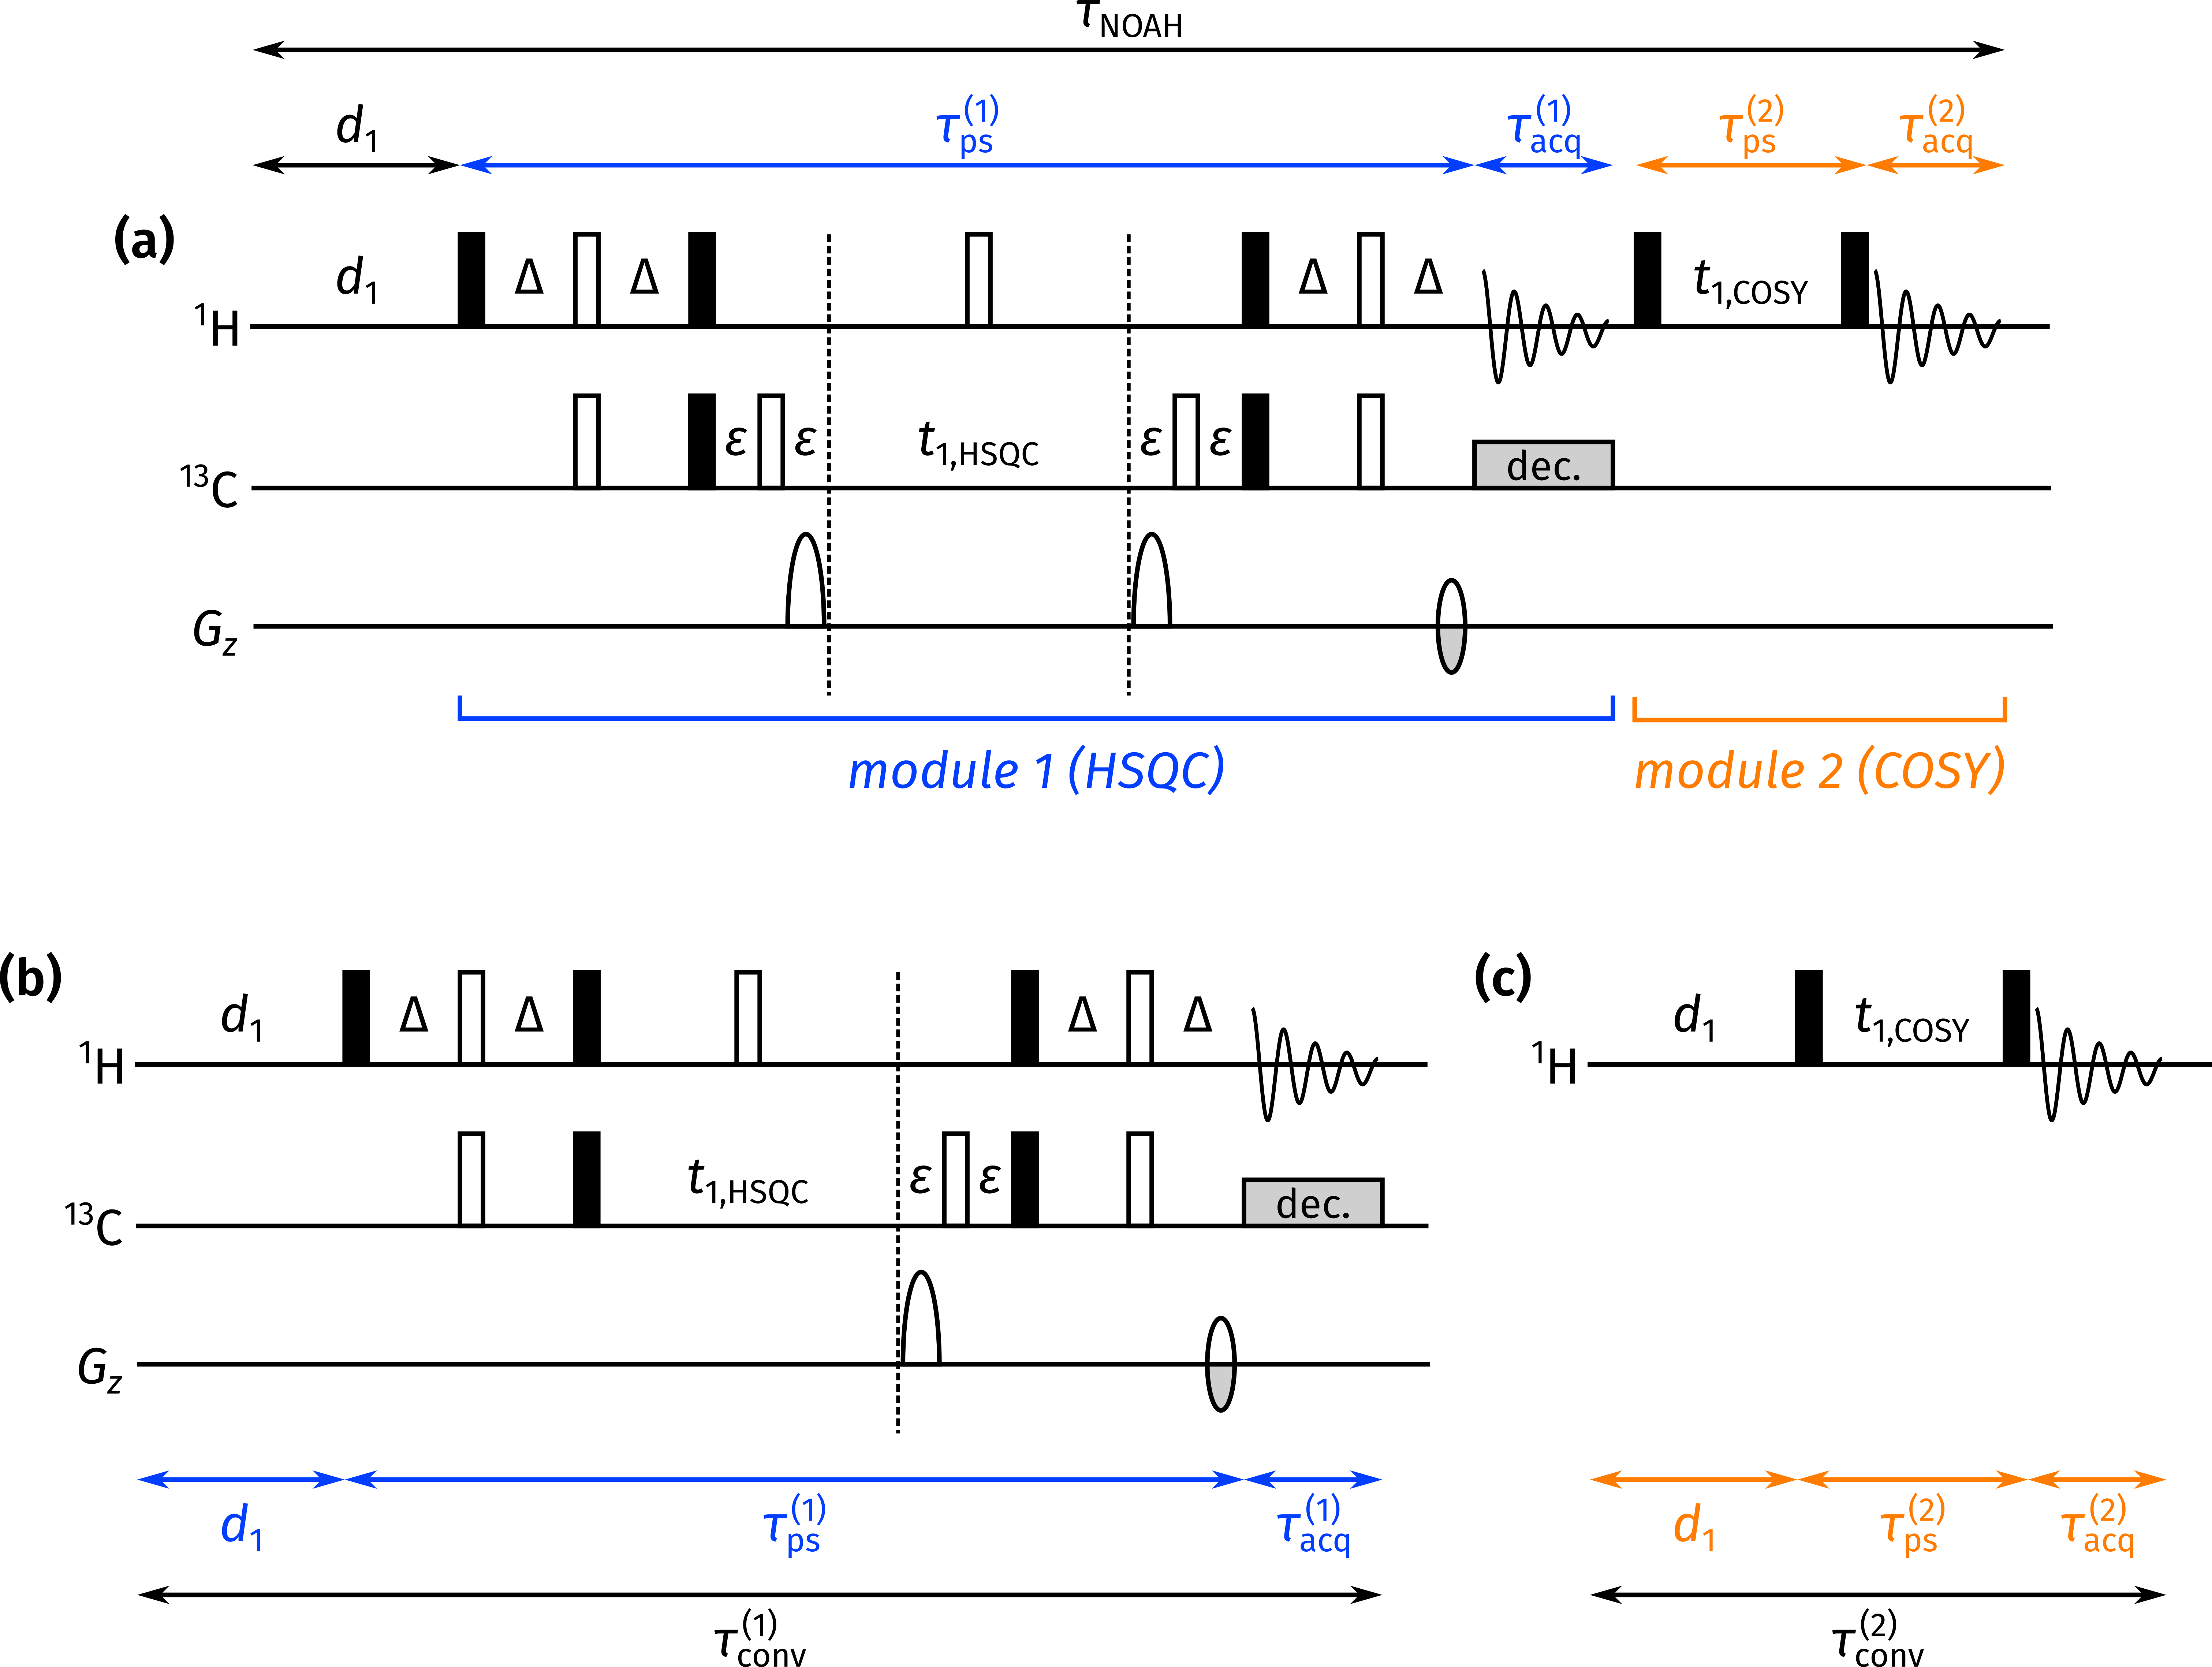
\includegraphics[]{noah/timings.png}%
    {\phantomsubcaption\label{fig:noah_timings_noah_sc}}%
    {\phantomsubcaption\label{fig:noah_timings_conv_s}}%
    {\phantomsubcaption\label{fig:noah_timings_conv_c}}%
    \caption[Comparison of NOAH and conventional 2D experiments]{
        \textbf{(\subref*{fig:noah_timings_noah_sc})} \noah{S,C} supersequence, comprising HSQC and COSY modules (see \cref{tbl:noah_modules} for an explanation of the single-letter module codes used).
        \textbf{(\subref*{fig:noah_timings_conv_s})} `Conventional' echo--antiecho HSQC (the same as in \cref{fig:hsqc_etgp}).
        \textbf{(\subref*{fig:noah_timings_conv_c})} `Conventional' COSY.
        The timings referred to in the text are highlighted for all three experiments; I have assumed that $d_1$ for each experiment is the same.
        Note that the lengths are not to scale: $d_1$ is typically far longer than the $\tau_\text{ps}$ and $\tau_\text{acq}$.
    }
    \label{fig:noah_timings}
\end{figure}

In a typical 2D NMR experiment, the majority of the experiment duration is taken up by the \textit{recovery delay}---the time required for spins to return to their equilibrium polarisation, such that the next transient or $t_1$ increment can be recorded.
The removal (or shortening) of recovery delays is thus a very effective way of speeding up 2D data acquisition.
In NOAH supersequences, 2D experiments (`modules') can be directly concatenated without the addition of extra recovery delays between them: only one overall recovery delay is required for the entire supersequence.
This means that, to a first approximation, a supersequence containing $N$ modules ($N \geq 2$) can be acquired in the time needed for just one module.
\Cref{fig:noah_timings} shows an example of a NOAH supersequence formed from two modules (HSQC and COSY): the various timings referred to in the text which follows are also marked on the diagram.

The duration of an NMR experiment, $\tau_\text{exp}$, can be expressed as a sum of its parts:
\begin{equation}
    \label{eq:exp_duration_2d}
    \tau_\text{exp} = \tau_\text{ps} + \tau_\text{acq} + d_1,
\end{equation}
where $\tau_\text{ps}$ is the time required for the pulse sequence itself (typically several milliseconds), $\tau_\text{acq}$ is the acquisition time (several hundred milliseconds), and $d_1$ is the recovery delay (one or more seconds).
The \textit{time-saving factor} $\rho_t$ for a NOAH supersequence, as compared to a series of conventional standalone experiments, is then:
\begin{equation}
    \label{eq:rho_t}
    \rho_t
    = \frac{\sum_i \tau_\text{conv}^{(i)}}{\tau_\text{NOAH}}
    = \frac{{\sum_i (\tau_\text{ps}^{(i)} + \tau_\text{acq}^{(i)} + d_1^{(i)})}}{d_1 + \sum_i (\tau_\text{ps}^{(i)} + \tau_\text{acq}^{(i)})},
\end{equation}
where $\tau_\text{NOAH}$ is the duration of the NOAH experiment, $\tau_\text{conv}$ is the duration of a conventional experiment, and the superscript $(i)$ represents the $i$-th module or conventional experiment being acquired.
The sum runs from $i = 1$ to $N$, where $N$ is the number of modules.
If we assume that $d_1^{(i)} = d_1$ is the same for all $N$ conventional experiments and the supersequence, then in the limit where
\begin{equation}
    \label{eq:d1_limit}
    d_1 \gg \sum_i \tau_\text{ps}^{(i)} + \tau_\text{acq}^{(i)},
\end{equation}
we have that $\rho_t \to Nd_1/d_1 = N$.
This analysis makes plenty of assumptions, and is not entirely valid in practice.
For example, \textit{each} $\tau_\text{acq}$ is often around 5\text{--}10\% of $d_1$, so is not entirely negligible, especially in longer supersequences.
Furthermore, some modules require longer $\tau_\text{ps}$: most notable is the NOESY module, which contains a mixing time of several hundred milliseconds. (HMBC, TOCSY, and ROESY spectra are also lesser offenders.)
These factors serve to reduce $\rho_t$ from its idealised value of $N$; generally, this deviation is larger as $N$ increases, because \cref{eq:d1_limit} becomes less and less valid.
Nevertheless, the general point that time savings are approximately proportional to $N$ stands.

For relatively concentrated samples, where sensitivity is not an issue, we can in fact end the discussion here.
In this \textit{sampling-limited regime}, the minimum 2D experiment duration is dictated purely by the number of $t_1$ increments needed to obtain sufficient resolution in the indirect dimension, as well as the minimum phase cycle required for artefact suppression.%
\footnote{With modern gradient-enhanced experiments, the minimum phase cycle may well not even be a `cycle'; see also \cref{fig:hsqc_comparison}.}
NOAH supersequences are identical to conventional experiments in both aspects, but provide a time-saving factor of $\rho_t \sim N$.

The development of modern NMR instrumentation, including high-field magnets and cryogenic probes, means that the sampling-limited regime continues to be extended to ever lower concentrations.
However, it is often not this simple: the opposite \textit{sensitivity-limited regime} is still very commonly encountered, for example with naturally insensitive experiments (e.g.\ ADEQUATE), low-field benchtop NMR, or most simply, dilute samples.%
\footnote{If the SNR factor $A^{(i)}$ as discussed below is \textit{very small}, then it is possible that even concentrated samples may be shifted into the sensitivity-limited regime. This is never really the case in practice, though, as will be shown in \cref{subsec:noah__case_studies}.}

In such cases, it becomes mandatory to compare the SNRs of the NOAH modules and conventional experiments.
To do so, we define for each module an \textit{SNR factor} $A^{(i)}$, which is the SNR of the NOAH module divided by the SNR of a conventional experiment, acquired with the same parameters.%
\footnote{The relative SNR will likely vary from peak to peak in the spectrum, and $A^{(i)}$ should in theory be quoted either as an average over all peaks, or as a range. This is what I have done in this thesis. However, comparisons in the literature are not always as thorough.}
In general, we have that $A \leq 1$, because NOAH modules frequently contain small modifications from conventional experiments (as will be explained in \cref{subsec:noah__magpools}).
The \textit{gain in sensitivity per unit time}, $\varepsilon^{(i)}$, is then defined by
\begin{equation}
    \label{eq:varepsilon_i}
    \varepsilon^{(i)} = A^{(i)} \sqrt{\rho_t},
\end{equation}
where the square root accounts for the fact that SNR scales only as the square root of the number of scans, or the number of times the experiment can be repeated in a given period.
Of course, the exact values calculated for $A^{(i)}$ (and hence $\varepsilon^{(i)}$) will depend on the sample chosen for the comparison.
These values should therefore be assumed to be valid only for similar samples.

If $\varepsilon^{(i)} > 1$, as is frequently the case, this means that the NOAH supersequence provides greater sensitivity per unit time in the $i$-th module compared to a standalone experiment.
Equivalently, performing a NOAH experiment allows data of sufficient sensitivity to be obtained in less time.
Naturally, this condition is most important for modules which are inherently insensitive, particularly heteronuclear correlation modules.
For sensitive (typically homonuclear) modules, it is often perfectly tolerable to have $A < 1$ or even $\varepsilon < 1$, as even with this sensitivity penalty they are still more intense than the heteronuclear modules.

Another issue with NOAH supersequences is that each module is run with the same number of scans (phase cycle).
Although this was touted as a benefit in the sampling-limited regime, this may in fact be undesirable in the sensitivity-limited regime, where insensitive experiments need to be run with more scans than sensitive ones.
In this case, the \textit{effective} time savings provided by NOAH experiments are smaller:
\begin{equation}
    \label{eq:rho_t_eff}
    \rho_{t,\text{eff}}
    = \frac{\sum_i \tau_\text{conv}^{(i)}}{\tau_\text{NOAH}}
    = \frac{{\sum_i S^{(i)}(\tau_\text{ps}^{(i)} + \tau_\text{acq}^{(i)} + d_1^{(i)})}}{Sd_1 + S\sum_i (\tau_\text{ps}^{(i)} + \tau_\text{acq}^{(i)})},
\end{equation}
where each standalone experiment is acquired with $S^{(i)}$ scans and the NOAH experiment with $S$ scans.
Typically, $S$ is simply the largest of the $S^{(i)}$.
If $S^{(i)} = S$ for all $i$, then \cref{eq:rho_t_eff} simply reduces to \cref{eq:rho_t}; on the other hand, if the $S^{(i)}$'s are different, then we have that $\rho_{t,\text{eff}} < \rho_t$.
In such a situation, it is probably more appropriate to describe a NOAH supersequence as `measuring the most insensitive module and getting the others for free'.
Indeed, if $S = S^{(i)} \gg S^{(j\neq i)}$, then `the other' modules require almost no time to measure (relative to the least sensitive module), and $\rho_{t,\text{eff}}$ tends towards 1, meaning that even the time-saving utility of NOAH vanishes.
A corollary of this is that NOAH supersequences are generally best constructed from modules which have similar intrinsic sensitivities and hence similar $S^{(i)}$'s.

As the reader can no doubt appreciate by now, the comparison of NOAH and conventional spectra is fraught with subtleties (which are sometimes glossed over in the literature, but invariably surface in real-life discussions).
In fact, it is hardly even difficult to construct yet more edge cases.
For example, one may not want to acquire all the individual spectra `conventionally': for example, NUS may be used for a HSQC experiment but not for others; or $d_1$ may be varied for different experiments.
These will have an impact on both the durations of the experiments, as well as their sensitivities.
To make any meaningful quantitative comparisons, it is therefore necessary to restrict the discussion to values of $\rho_t$, $A$, and $\varepsilon$, which can be objectively calculated.
This is the approach I have taken in this thesis.
These should of course be read with the qualitative understanding that depending on the context, these aforementioned factors may lead to \textit{some}---but never a \textit{complete}---decrease in the utility of NOAH experiments.

\subsection{Magnetisation pools}
\label{subsec:noah__magpools}

Having gotten this relatively dry material out of the way, I now turn to exactly how NOAH supersequences are constructed.
Ordinarily, if the recovery delay is removed from an NMR experiment, its sensitivity will be greatly reduced because insufficient magnetisation will have recovered between repetitions; or in other words, $A^{(i)}$ will be very small.
Such experiments would only really be useful well in the sampling-limited regime.

The key to avoiding this in NOAH supersequences is to make sure that \textit{each module samples a different source of magnetisation}.
For example, a HSQC module can be designed to only sample magnetisation of protons directly bonded to the 1.1\%-natural abundance \carbon{}, and leave all other proton magnetisation untouched.
Immediately following this, the remainder of the proton magnetisation can then be used to record (say) a COSY module, without needing a separate recovery delay.
Using the notation of Orts and Gossert\autocite{Orts2018M}, the magnetisation of \carbon{}--bound protons is denoted as \magn{C}, and the magnetisation of protons \textit{not} bonded to \carbon{} is denoted as \magnnot{C}.
Protons not directly bonded to NMR-active heteronuclei are labelled \magnnot{X}, and will often be referred to as `bulk' magnetisation, since (in natural-abundance samples) the majority of protons fall into this category.

Most standard 2D experiments do not preserve unused magnetisation but instead dephase it through CTP gradient selection; thus, NOAH modules often require some modifications compared to standard experiments.
For example, compared to the echo--antiecho HSQC (discussed in \cref{subsec:theory__hsqc_ea}), the NOAH HSQC module\autocite{Kupce2017ACIE} adds an extra CTP gradient so that the bulk magnetisation is refocused and ultimately returned to the $+z$ equilibrium state (\cref{fig:noah_sb_po_s}).
(This is largely identical to the `symmetrised' ASAP-HSQC experiment\autocite{SchulzeSunninghausen2017JMR}.)

\begin{figure}[htb]
    \centering
    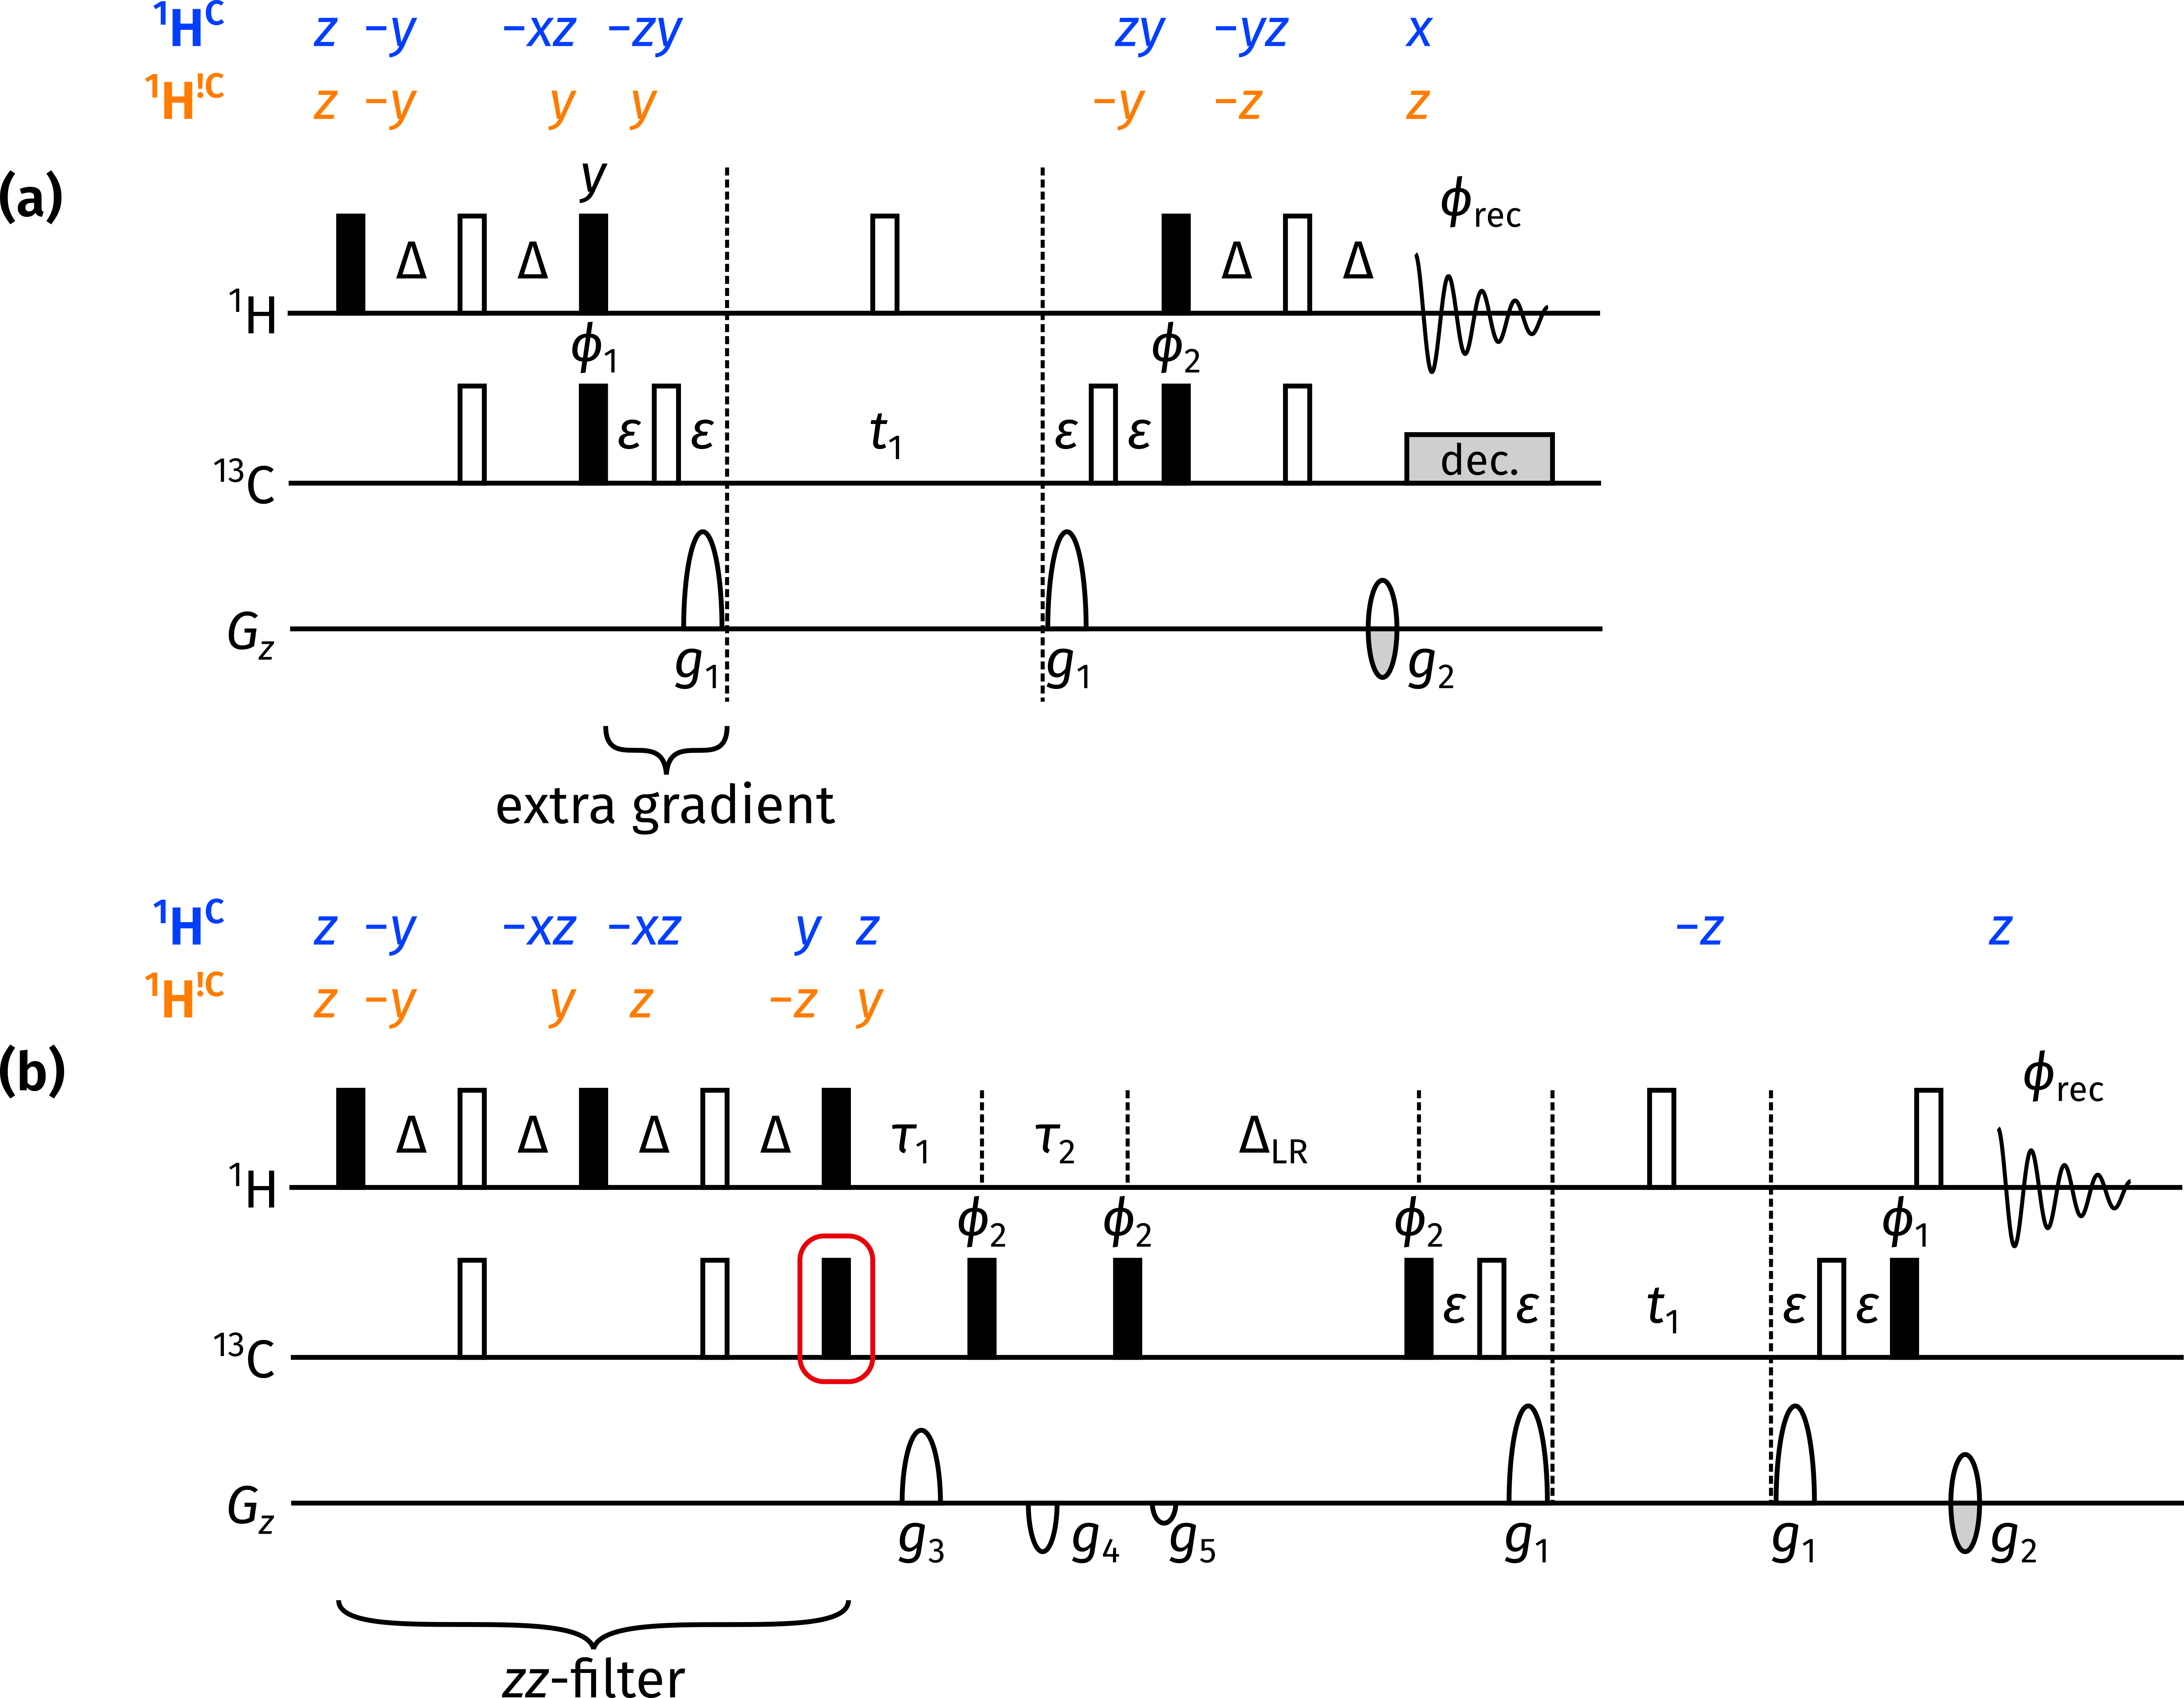
\includegraphics[]{noah/hsqc_hmbc_prodops.png}%
    {\phantomsubcaption\label{fig:noah_sb_po_s}}%
    {\phantomsubcaption\label{fig:noah_sb_po_b}}%
    \caption[NOAH HSQC and HMBC modules with product operator analysis]{
        \textbf{(\subref{fig:noah_sb_po_s})} 
        NOAH HSQC module.
        \textbf{(\subref{fig:noah_sb_po_b})} 
        NOAH HMBC module.
        The \ang{90} pulse highlighted in red is described in \cref{subsec:noah__hmbc}.
        Delays are set as: $\Delta = 1 / (4 \cdot \oneJ{CH})$; $\Delta_\text{LR} = 1 / (2 \cdot \nJ{CH})$; $\tau_1 = 1 / (2 \cdot \oneJ{CH,\text{max}})$; $\tau_2 = 1 / (2 \cdot \oneJ{CH,\text{min}})$ (see also \cref{subsec:poise__hmbc} for the LPJF).
        Phase cycling is performed with $\phi_1 = (x, -x)$, $\phi_2 = (x, x, -x, -x)$, and $\phi_\text{rec} = (x, -x, -x, x)$.
        Gradient amplitudes are $(g_1, g_2, g_3, g_4, g_5) = (80\%, \pm 40.2\%, 15\%, -10\%, -5\%)$.
        Product operator analysis is provided above both modules for both the \magn{C} and \magnnot{C} magnetisation pools; the notation for this is explained in the \textit{Preface}.
    }
    \label{fig:noah_sb_po}
\end{figure}

Sometimes, the modifications required are more extensive, as in the HMBC module.
If this module is followed by a HSQC module (or any other module which draws on \magn{C} magnetisation), the initial \ang{90} excitation pulse must be replaced with a $zz$-filter (\cref{fig:noah_sb_po_b}).
This performs an \textit{isotope-selective rotation} in that \magn{C} magnetisation is stored along the $z$-axis, but \magnnot{C} magnetisation is excited (and subsequently detected).
In general, sequences which are thus modified have lower sensitivities (i.e.\ $A < 1$) than the `original' sequences from which they were derived.
This is partly because of imperfect manipulation of magnetisation by the extra pulse sequence elements, and also increased losses due to relaxation during these extended sequences.

In contrast, modules placed towards the \textit{end} of a supersequence do not need to be modified, as they do not need to preserve any magnetisation.
This includes virtually all homonuclear modules, which are allowed to simply consume any remaining magnetisation.
Although this makes their implementation very straightforward, in general these modules will \textit{also} suffer some losses in sensitivity, because the preceding modules do not perfectly retain all magnetisation.

Thus, in general, it is not possible for any module in a NOAH supersequence to have $A = 1$, unless it is placed first in the supersequence \textit{and} has not undergone any modifications.%
\footnote{Of course, this also depends on exactly \textit{what} standalone experiment the NOAH supersequence is being compared against. Sometimes, in the literature, the NOAH experiment has been compared against its constituent modules acquired in a standalone fashion; in this case, the first module will always have $A = 1$. This tells us how much we gain through the act of concatenating modules, but is less meaningful in the `real world' where one is interested in how useful NOAH is relative to `typical' optimised 2D experiments. I therefore prefer to make comparisons against standard-library sequences.}
Such cases are very rare, and it is thus necessary to accept some decreases in $A$, which are often fairly small (on the order of 10--20\%).
In the sampling-limited regime, sensitivity is not at a premium and this is often perfectly tolerable.
In the sensitivity-limited regime, the full time savings $\rho_t$ cannot be realised, but since $\varepsilon$ is still typically larger than 1, there is still an overall boost in sensitivity per unit time.

\subsection{Case studies}
\label{subsec:noah__case_studies}

Using all that has been described in the previous sections, we now look at a few `typical' supersequences to understand their construction.
A quick note about the nomenclature of NOAH supersequences is warranted here.
Supersequences are labelled by the number of modules $N$, plus a series of single-letter codes corresponding to the identity and ordering of the modules involved (\cref{tbl:noah_modules}).
Occasionally, superscripts or subscripts are used to qualify the modules involved.%
\footnote{With the increasing number of modules, and the variety of modern NMR experiments which could be incorporated into NOAH supersequences, keeping these abbreviations short yet meaningful has been a challenge.}
Thus, a NOAH supersequence containing three modules---say \nitrogen{} HMQC, \carbon{} HSQC, and CLIP-COSY---would be referred to as a \noah{Mn,S,Cc}.
\Cref{tbl:noah_sensitivities} provides values of $\rho_t$ and $A$ for each module of several typical supersequences, which will be rationalised in the text which follows.

\begin{table}[!ht]
    \begin{tabular}{cccccc}
        \toprule
        \multicolumn{2}{c}{\textbf{\proton{}--\nitrogen{} modules}}  &
        \multicolumn{2}{c}{\textbf{\proton{}--\carbon{} modules}}    &
        \multicolumn{2}{c}{\textbf{\proton{}--\proton{} modules}}   \\
        \cmidrule(lr){1-2}
        \cmidrule(lr){3-4}
        \cmidrule(lr){5-6}
        Module & Code        & Module     & Code           & Module     & Code       \\
        \midrule
        HMQC   & \noah*{Mn}  & HSQC       & \noah*{S}      & COSY       & \noah*{C}  \\
        HSQC   & \noah*{Sn}  & seHSQC     & \noah*{Sp}     & CLIP-COSY  & \noah*{Cc} \\
        seHSQC & \noah*{Spn} & HSQC-TOCSY & \noah*{St}     & DQF-COSY   & \noah*{D}  \\
        HMBC   & \noah*{Bn}  & HSQC-COSY  & \noah*{Sc}     & TOCSY      & \noah*{T}  \\
               &             & 2BOB       & \noah*{O}      & NOESY      & \noah*{N}  \\
               &             & HMBC       & \noah*{B}      & ROESY      & \noah*{R}  \\
               &             & ADEQUATE   & \noah*{A}      & PSYCHE     & \noah*{P}  \\
               &             &            & \hspace{1.5cm} & TSE-PSYCHE & \noah*{Pt} \\
               &             &            &                & PSYCHE 2DJ & \noah*{J}  \\
        \bottomrule
    \end{tabular}
    % The hspace is to make the two subcolumns look more balanced.
    \caption[List of single-letter NOAH module codes]{
        A (non-exhaustive) list of single-letter module codes for a selection of NOAH modules.
        Note that, in the literature, the \nitrogen{} HMQC module has been referred to simply by `M', since the HSQC module is preferred for \proton{}--\carbon{} correlations.
        In this thesis, I include the subscript N throughout to avoid any ambiguity.
    }
    \label{tbl:noah_modules}
\end{table}

\begin{table}[!ht]
    % data is in lab book: noah-misc/220224/
    \begin{tabular}{ccccccccc}
        \toprule
        \textbf{Entry} & \textbf{Sequence} & $\symbf{\tau}_{\textbf{NOAH}}$ & $\symbf{\rho}_{\symbfit{t}}$ & \multicolumn{5}{c}{$\symbfit{A}$} \\
        \cmidrule(lr){5-9}
        & & & & HMBC & seHSQC & HSQC & COSY & TOCSY \\
        \midrule
        1 & \noah*{S,C}         & 15 min 0 s  & 1.87 &      &      & 0.97 & 0.90 &      \\
        2 & \noah*{S,C,T}       & 16 min 25 s & 2.60 &      &      & 1.01 & 0.99 & 0.79 \\
        3 & \noah*{B,S}         & 15 min 40 s & 1.82 & 0.93 &      & 0.87 &      &      \\
        4 & \noah*{S,B}         & 15 min 35 s & 1.83 & 0.99 &      & 0.96 &      &      \\
        5 & \noah*{B,S,C,T}     & 17 min 48 s & 3.22 & 0.95 &      & 0.90 & 0.36 & 0.28 \\
        6 & \noah*{B,Spn,S,C,T} & 18 min 57 s & 3.74 & 0.95 & 0.71 & 0.66 & 0.38 & 0.30 \\
        7 & \noah*{Spn,B,S,C,T} & 18 min 56 s & 3.75 & 0.76 & 0.79 & 0.74 & 0.33 & 0.26 \\
        \bottomrule
    \end{tabular}
    \caption[Sensitivity and time-saving analyses of several NOAH supersequences]{
        Sensitivity and time-saving analyses of several typical NOAH supersequences.
        All experiments were acquired with 2 scans per increment, 256 $t_1$ increments, an acquisition time of \qty{67}{\ms}, and a recovery delay of \qty{1.5}{\s}.
        The HMBC module used here includes the extra \carbon{} \ang{90} pulse described later in \cref{subsec:noah__hmbc}: this has no significant impact on the SNR, and is only mentioned as a technicality.
        The \nitrogen{} seHSQC module is that described in \cref{subsec:noah__sehsqc_n}.
        The CT module here was run with States indirect-dimension quadrature detection, and the individual C module (in entry 1) with echo--antiecho.
        The following Bruker library sequences were used as the `conventional' experiments: \texttt{hmbcetgpl2nd}, \texttt{hsqcetf3gpsi2}, \texttt{hsqcetgpsp.2}, \texttt{cosygpqf}, and \texttt{dipsi2gpphzs}.
        \datacode{7Z-220224}
    }
    \label{tbl:noah_sensitivities}
\end{table}

\subsubsection{\noah{S,C}: HSQC + COSY}

We begin with perhaps the simplest example of a NOAH supersequence, one containing the HSQC and COSY modules: this is labelled as a \noah{S,C} experiment (entry 1, \cref{tbl:noah_sensitivities}).
As shown in \cref{fig:noah_sb_po_s}, the HSQC module only samples \magn{C} magnetisation, and leaves \magnnot{C} magnetisation along the $+z$-axis
Although the HSQC experiment has to be modified to preserve this \magnnot{C} magnetisation, its sensitivity is practically unaffected as compared to a `standard' HSQC ($A = 0.97$).
Furthermore, the COSY module retains \textit{most} of its sensitivity ($A = 0.90$).
The small loss here is because the HSQC module does not \textit{perfectly} preserve the \magnnot{C} magnetisation: for example, evolution of J-couplings as well as relaxation occur during the HSQC pulse sequence, which are ignored in the product operator analysis in \cref{fig:noah_sb_po_s}.

The value of the time-saving factor, $\rho_t = 1.87$, is very close to the theoretical limit of $N = 2$.
This reflects the fact that the pulse sequence itself, $\tau_\text{ps}$, is fairly short for both the HSQC and COSY modules; the deviation therefore chiefly arises from the acquisition time, $\tau_\text{acq}$.
In all respects, this is therefore an example of an `ideal' NOAH supersequence, where the combination of two modules provides time savings without compromising on sensitivity.

It is worth pointing out that the order of the modules cannot be reversed: the COSY module cannot be (easily) modified to preserve \magn{C} magnetisation.
In a hypothetical \noah{C,S} supersequence, the later HSQC module would only be able to use magnetisation recovered during the COSY FID, leading to substantial sensitivity drops.

\begin{figure}[!ht]
    \centering
    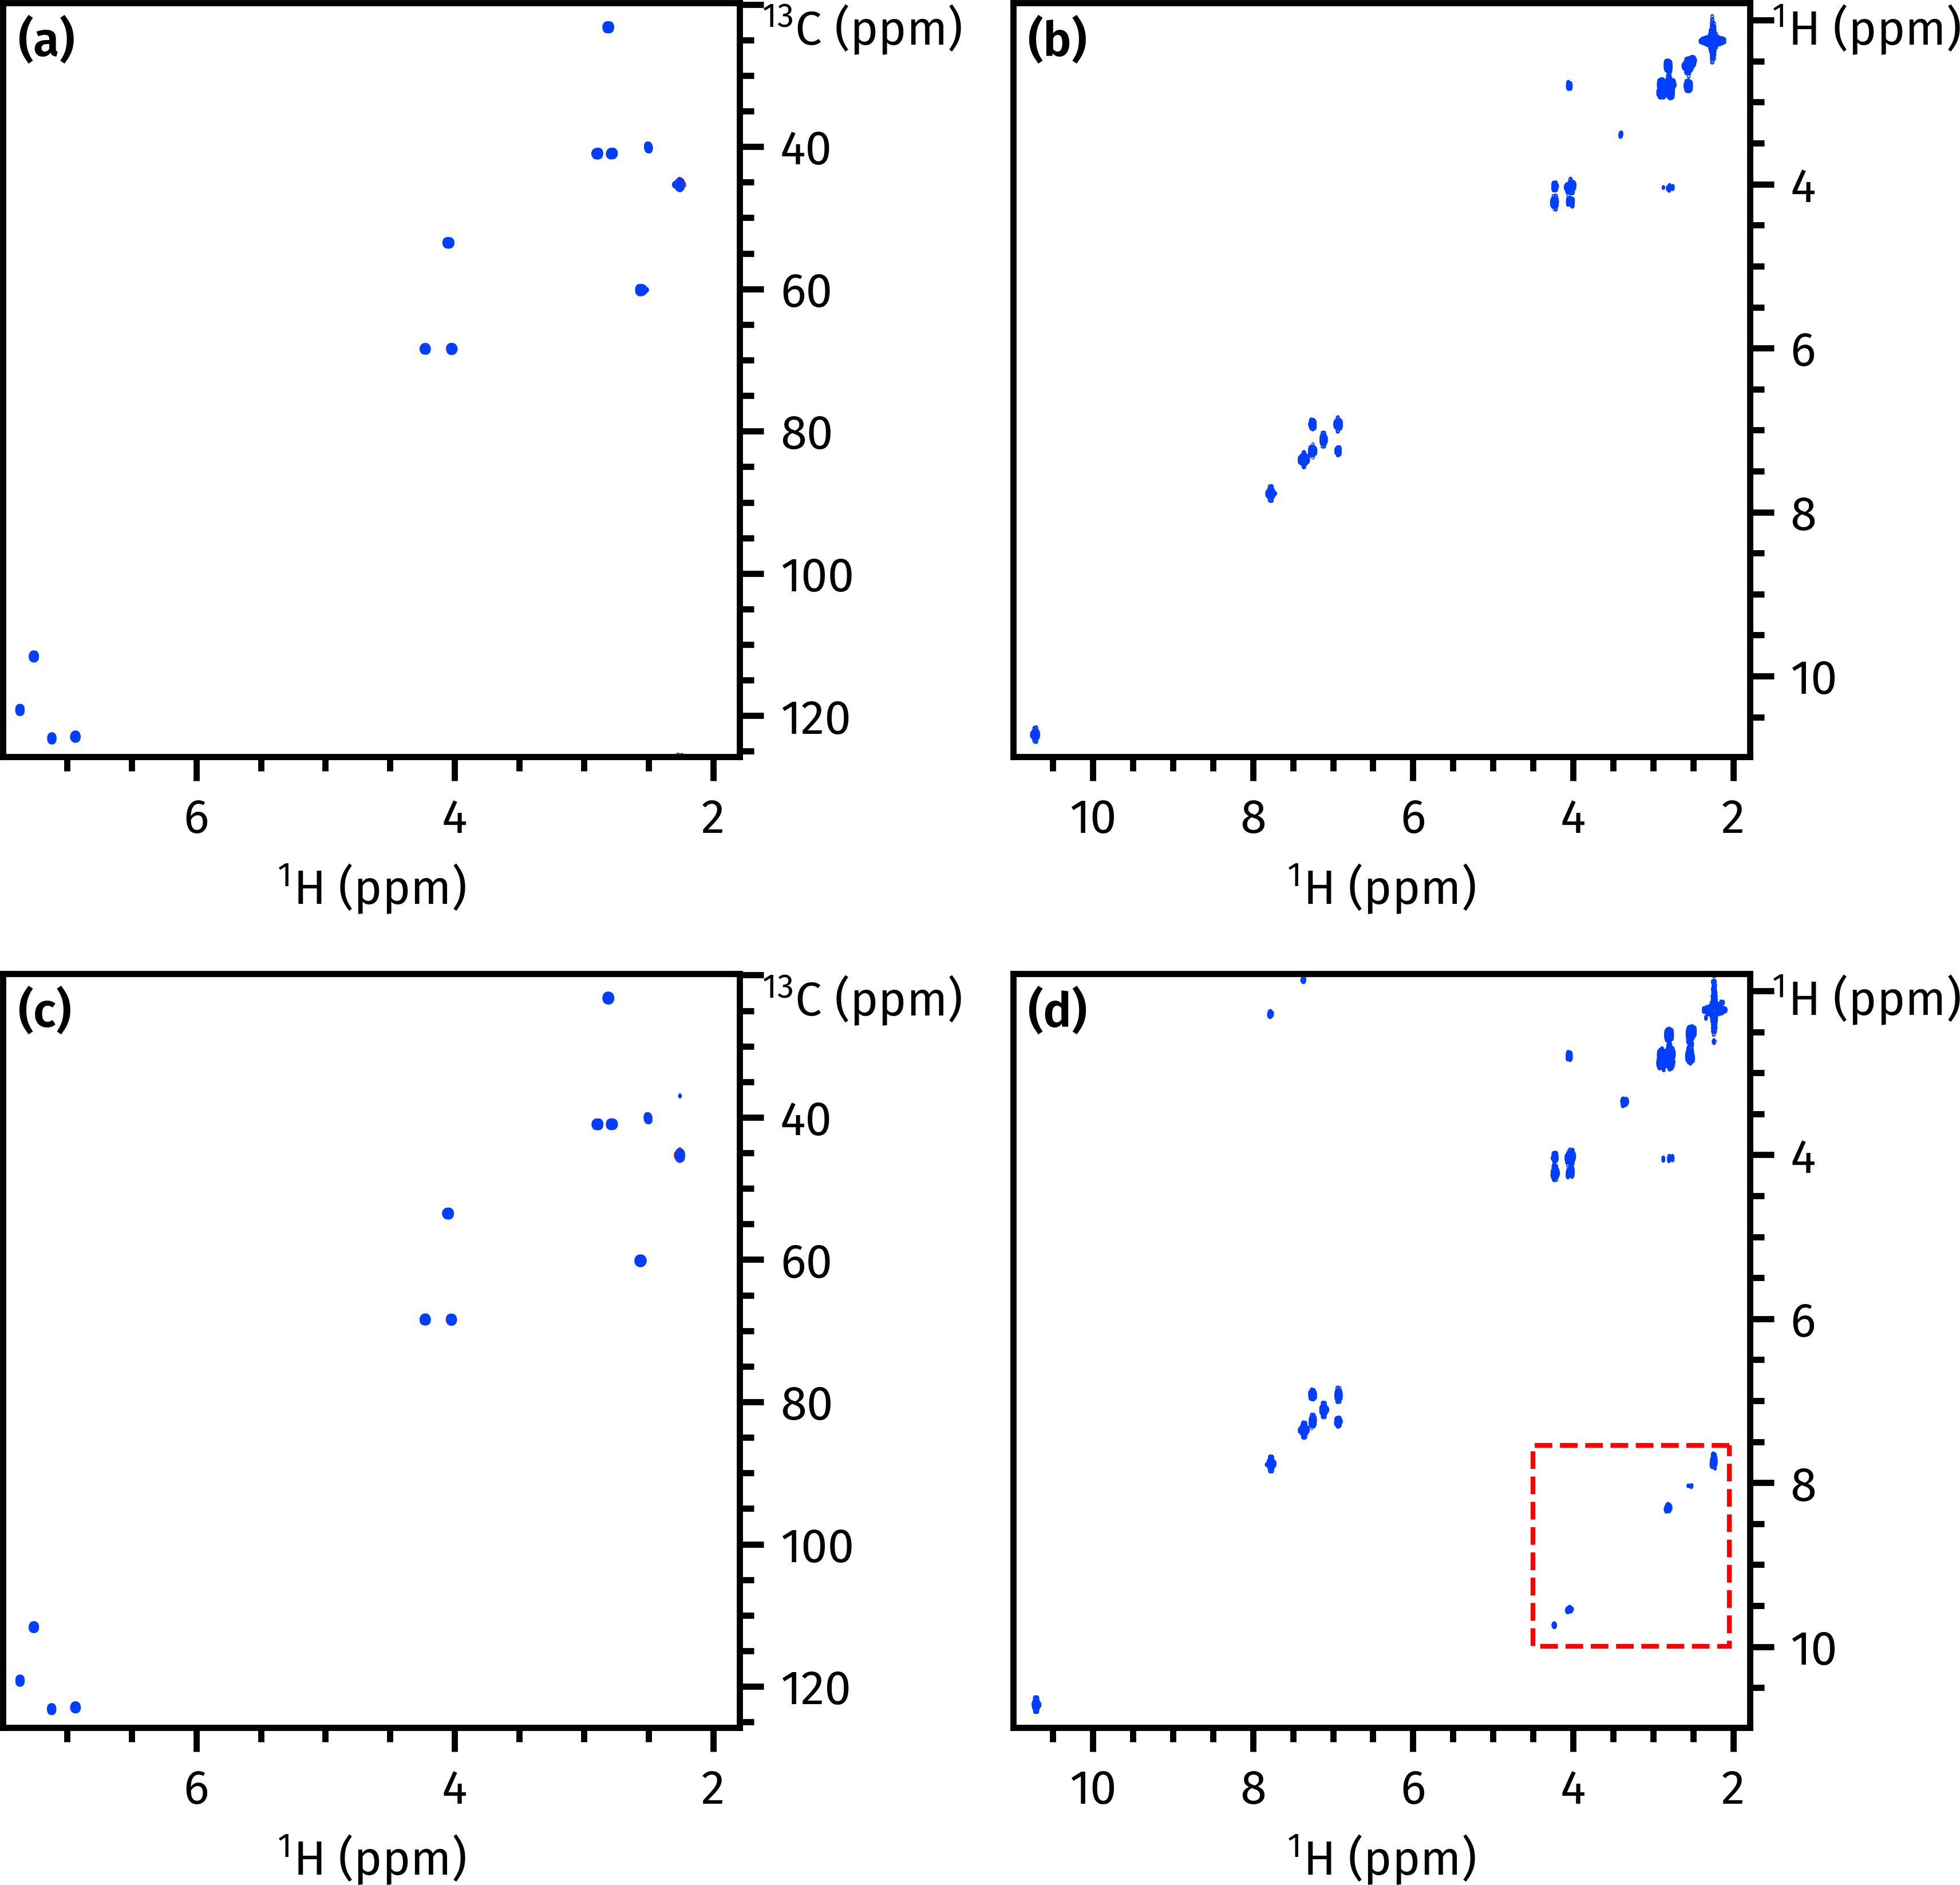
\includegraphics[]{noah/sc_noah_vs_conv.png}%
    {\phantomsubcaption\label{fig:sc_noah_vs_conv_noah_s}}%
    {\phantomsubcaption\label{fig:sc_noah_vs_conv_noah_c}}%
    {\phantomsubcaption\label{fig:sc_noah_vs_conv_conv_s}}%
    {\phantomsubcaption\label{fig:sc_noah_vs_conv_conv_c}}%
    \caption[Comparison of spectra obtained from \noah{S,C} and standalone experiments]{
        \textbf{(\subref*{fig:sc_noah_vs_conv_noah_s})} HSQC from \noah{S,C} supersequence.
        \textbf{(\subref*{fig:sc_noah_vs_conv_noah_c})} COSY from \noah{S,C} supersequence.
        \textbf{(\subref*{fig:sc_noah_vs_conv_conv_s})} Standalone HSQC.
        \textbf{(\subref*{fig:sc_noah_vs_conv_conv_c})} Standalone COSY; off-diagonal artefacts are highlighted in the red box.
        \datacode{7Z-220224}
    }
    \label{fig:sc_noah_vs_conv}
\end{figure}

A final point to consider would be whether the NOAH data has comparable spectral quality in terms of (for example) artefacts.
In this case, the answer is yes: the NOAH HSQC spectrum is virtually identical to the standalone (\cref{fig:sc_noah_vs_conv_noah_s,fig:sc_noah_vs_conv_conv_s}; both spectra have low-level artefacts of different kinds, which do not seriously impede the interpretation and are not shown).
On the other hand, the NOAH COSY spectrum seems to actually \textit{improve} on the standalone COSY, in that it better suppresses off-diagonal artefacts (\cref{fig:sc_noah_vs_conv_noah_c,fig:sc_noah_vs_conv_conv_c}).
These artefacts likely arise in the standalone COSY because of accidental refocusing of magnetisation which has not completely relaxed between $t_1$ increments.\autocite{Vitorge2010JMR}
In contrast, the NOAH COSY module has an extra set of HSQC gradients between every repetition of the COSY, so accidental refocusing is less likely.
(Similar artefacts have been noted before in the DQF-COSY experiment\autocite{Shaw1996JMRSA,Howe2014MRC}, and have also shown to be attenuated in the corresponding NOAH module\autocite{Claridge2019MRC}.)
That said, such improvements are not always guaranteed: there are sometimes artefacts which arise uniquely in NOAH experiments, some of which are discussed in the following sections.


\subsubsection{\noah{S,C,T}: HSQC + COSY + TOCSY}

Evidently, the fact that the HSQC preserves almost all \magnnot{C} magnetisation means that \textit{any} homonuclear module---or a combination thereof---can be placed after it.
In general, since homonuclear modules tend to consume any remaining bulk magnetisation, it is very difficult to create combinations of homonuclear modules which do not lead to significant reductions in sensitivity.
The only real exceptions are COSY/X combinations, where X can be NOESY, ROESY, or TOCSY: instead of concatenating the COSY and X modules, the COSY pulse sequence can instead be nested \textit{within} the X module, as was first demonstrated with X = NOESY\autocite{Haasnoot1984JMR,Gurevich1984JMR}.
Here, we use the COSY/TOCSY combination as an example.\autocite{Nolis2019MRC}
The COSY, TOCSY, and combined COSY/TOCSY modules are shown in \cref{fig:ct_states}.

\begin{figure}[!ht]
    \centering
    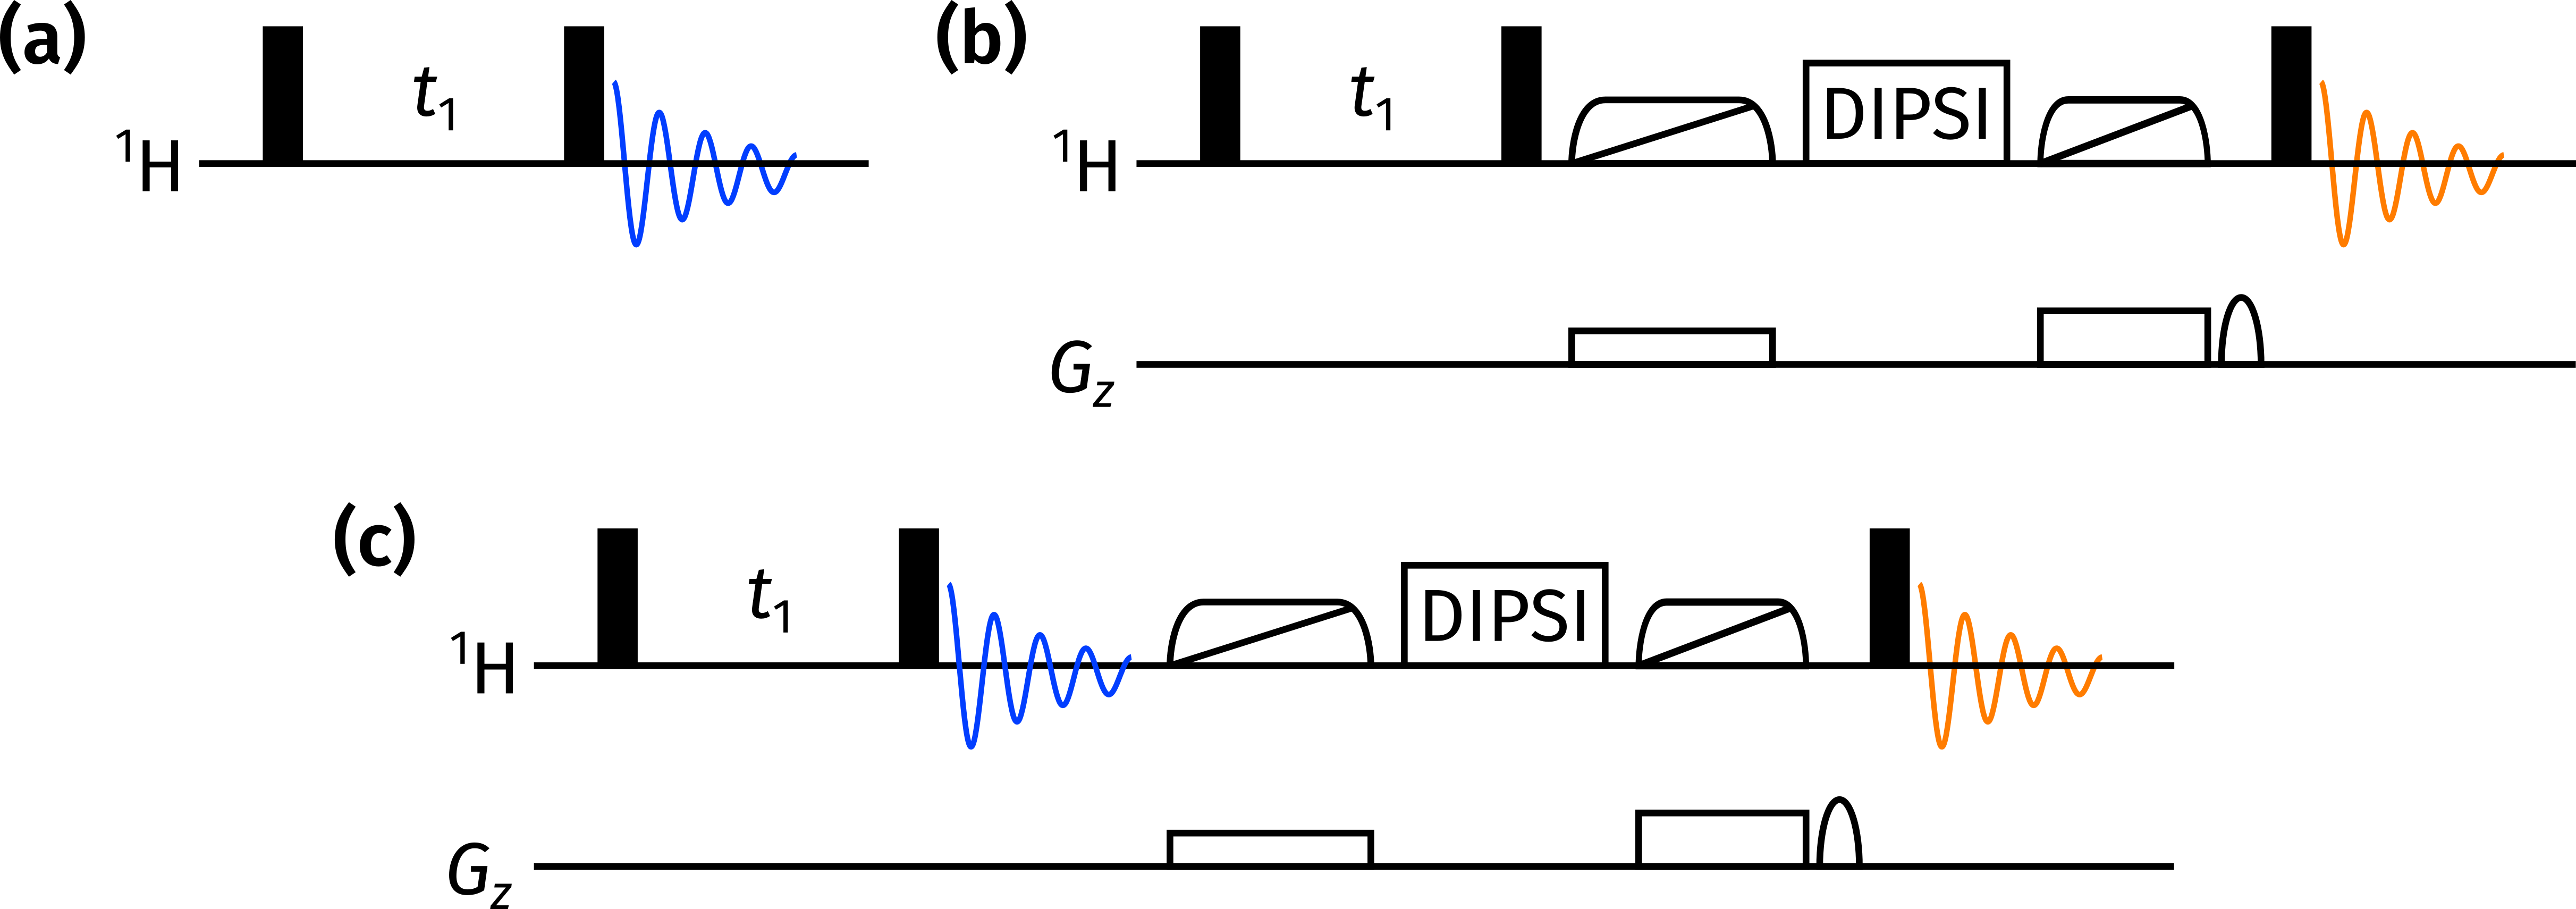
\includegraphics[]{pp/ct_states.png}%
    {\phantomsubcaption\label{fig:ct_states_c}}%
    {\phantomsubcaption\label{fig:ct_states_t}}%
    {\phantomsubcaption\label{fig:ct_states_ct}}%
    \caption[COSY/TOCSY NOAH module]{
        \textbf{(\subref*{fig:ct_states_c})} COSY module.
        \textbf{(\subref*{fig:ct_states_t})} TOCSY module; zero-quantum suppression is employed before and after the isotropic mixing period.
        \textbf{(\subref*{fig:ct_states_ct})} Combined COSY/TOCSY module, where the COSY FID is acquired immediately before the TOCSY mixing.
    }
    \label{fig:ct_states}
\end{figure}

As shown in \cref{tbl:noah_sensitivities} (entry 2), this nesting of the COSY module does not materially affect the TOCSY sensitivity.
A small loss of approximately 20\% is observed, which is partly due to the imperfect magnetisation preservation by the HSQC, and perhaps also due to relaxation during the COSY acquisition period.
As for the time-saving factor, a slightly larger deviation ($\rho_t = 2.60$) is observed from the ideal value of $3$.
This reflects the addition of a TOCSY mixing period, which contributes to $\tau_\text{ps}$.

\subsubsection{\noah{B,S}: HMBC + HSQC}

As mentioned previously, the HMBC module shown in \cref{fig:noah_sb_po_b} is designed to retain \magn{C} magnetisation through the addition of the $zz$-filter.
This can be used in a subsequent HSQC module in a \noah{B,S} supersequence.
Entry 3 of \cref{tbl:noah_sensitivities} shows that the addition of the $zz$-filter to the HMBC causes a relatively small 7\% decrease in sensitivity; on the other hand, the HSQC loses 13\% of its sensitivity because of incomplete magnetisation preservation.

Generally, it has been recommended that less sensitive modules are placed earlier in the supersequence so that they can access a larger proportion of the equilibrium magnetisation.
Since the HMBC is less sensitive of the two modules, this rule of thumb suggests that the BS supersequence would be better than the alternative SB supersequence.
In fact, the opposite is true, as entry 4 of \cref{tbl:noah_sensitivities} shows.
The HSQC module has a boost in sensitivity because it is placed first in the supersequence, and no longer needs to rely on the \magn{C} magnetisation preserved by the HMBC; and the HMBC also benefits because the $zz$-filter modification is no longer needed.%
\footnote{In fact, the final \ang{180} pulse in the HMBC module could also be removed: this is likely to give a further boost in SNR, as discussed in \cref{subsec:noah__hmbc}. However, this was not done here.}
Arguably, the ordering of modules in a supersequence should be considered on a case-by-case basis.

\subsubsection{\noah{B,S,C,T}: HMBC + HSQC + COSY + TOCSY}

We now move on to a longer supersequence containing four modules, with a correspondingly larger $\rho_t$ value of 3.22.
The sensitivity of the HSQC module is practically the same as in the \noah{B,S} supersequence just described: however, the COSY and TOCSY modules expose one weakness of the HMBC module which has so far been overlooked.
In principle, the HMBC module should only excite magnetisation of protons which are long-range coupled to \carbon{} (which we could, for example, denote as \magn{C(LR)}).
This magnetisation pool should be separate from both the directly coupled protons (\magn{C}), as well as protons which are not coupled to any \carbon{} at all (\magnnot{C}).
Unfortunately, this is not the case: it is not actually possible to separate the \magn{C(LR)} and \magnnot{C} magnetisation pools.
The HMBC excites both of these magnetisation sources, dephases the latter using CTP gradients, and detects the signal arising from the former.

What this means, of course, is that the COSY/TOCSY module which rely on \magnnot{C} magnetisation will have substantially lower sensitivities.
The signal detected in these two modules derives only from whatever has recovered during the previous two acquisition periods, as shown in entry 5 of \cref{tbl:noah_sensitivities}: $A$ for COSY and TOCSY is 0.36 and 0.28 respectively.
That said, this is in fact not likely to be an issue \textit{even} for sensitivity-limited samples.
Because the intrinsic sensitivity of the HMBC is orders of magnitude lower than the COSY and TOCSY, even with these large losses in sensitivity, the COSY and TOCSY spectra still have greater intensities than the HMBC.
Thus, as long as the entire supersequence is acquired with enough scans to make the HMBC SNR sufficient, the SNR in the COSY and TOCSY will \textit{also} be acceptable.
This is illustrated in \cref{fig:bsct}.

A rather more insidious problem is that different signals relax at different rates: thus, the COSY and TOCSY spectra (or indeed, any homonuclear module) will have uneven intensities and are frequently asymmetric.
This can be seen in the COSY spectrum, where a pair of asymmetric crosspeaks are highlighted.
Adding a period of isotropic mixing before the COSY module\autocite{Kupce2018CC} can help to ameliorate this to some extent (this was not performed when acquiring the data in \cref{fig:bsct}).

\begin{figure}[!ht]
    \centering
    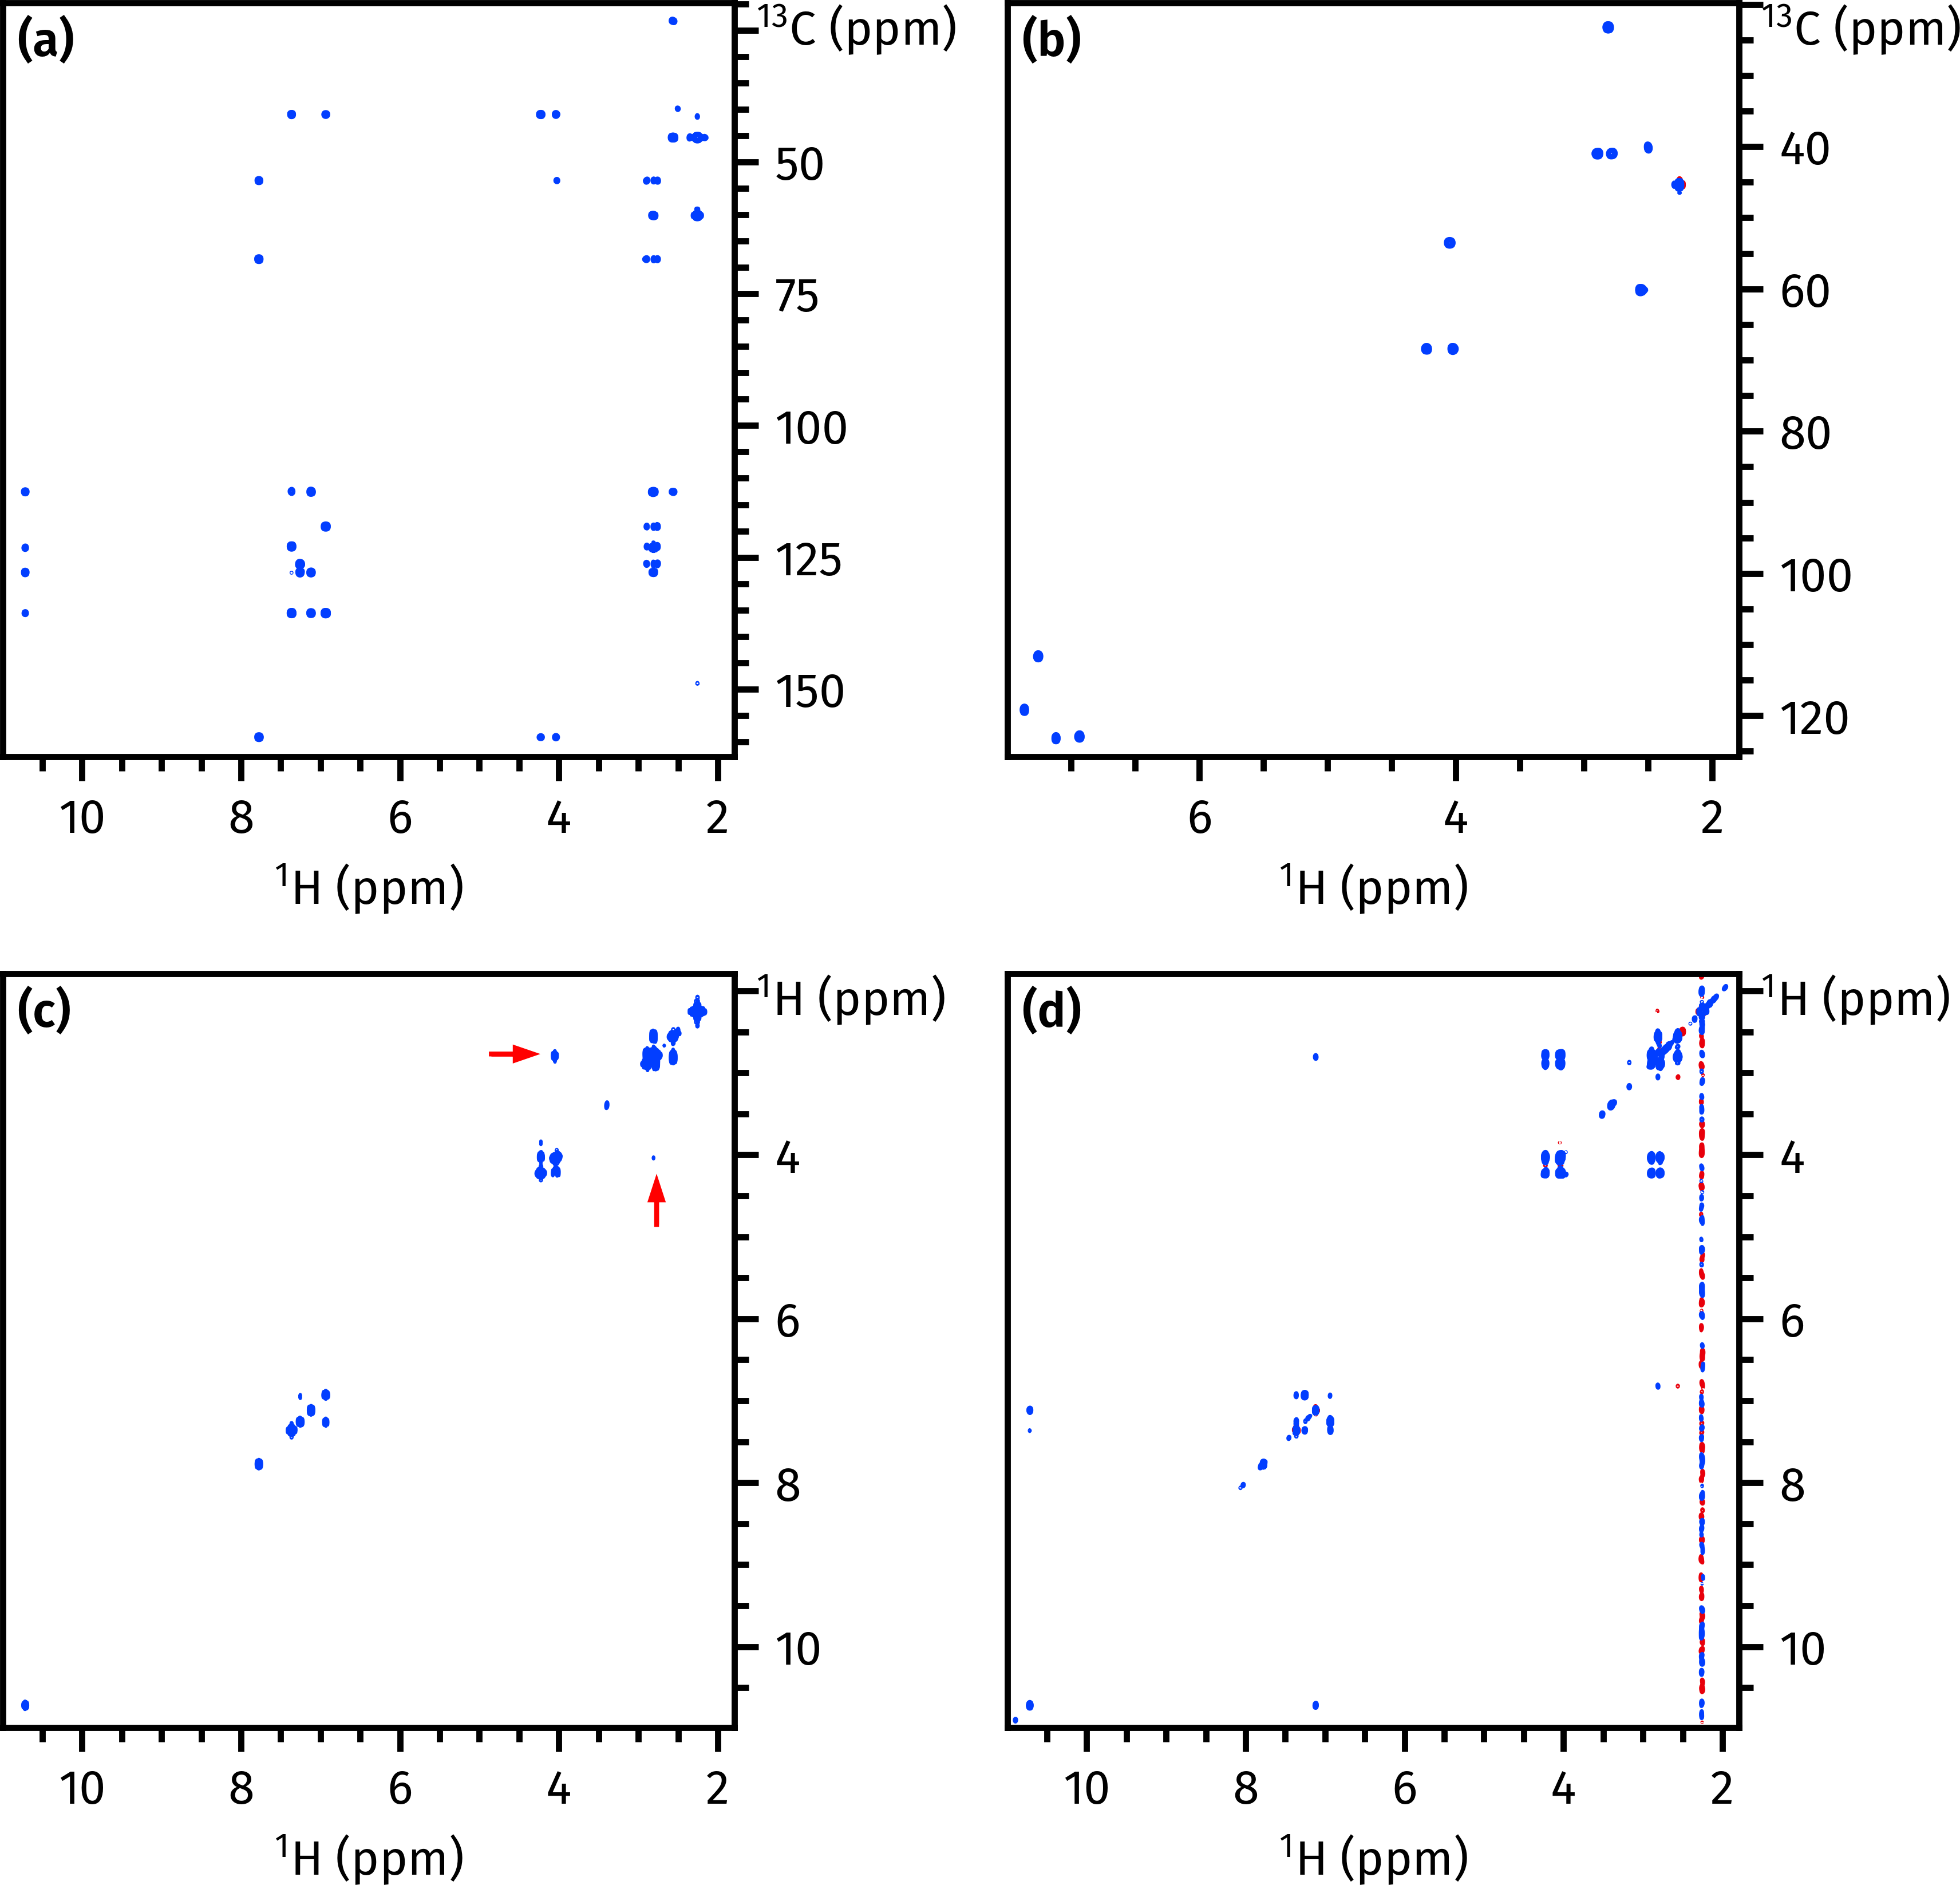
\includegraphics[]{noah/bsct.png}%
    {\phantomsubcaption\label{fig:bsct_b}}%
    {\phantomsubcaption\label{fig:bsct_s}}%
    {\phantomsubcaption\label{fig:bsct_c}}%
    {\phantomsubcaption\label{fig:bsct_t}}%
    \caption[Spectra obtained from a \noah{B,S,C,T} supersequence.]{
        Spectra obtained from a \noah{B,S,C,T} supersequence. 
        \textbf{(\subref*{fig:bsct_b})} HMBC.
        \textbf{(\subref*{fig:bsct_s})} HSQC.
        \textbf{(\subref*{fig:bsct_c})} COSY; a pair of asymmetric crosspeaks are highlighted with red arrows.
        \textbf{(\subref*{fig:bsct_t})} TOCSY (\qty{60}{\ms} DIPSI-2 mixing).
        Despite the COSY and TOCSY having only around 30\% of their sensitivity compared to standalone experiments, the intensity of the spectra obtained is still perfectly acceptable (the contour levels chosen are 1--2 orders of magnitude larger than for the HMBC).
        \datacode{7Z-220224}
    }
    \label{fig:bsct}
\end{figure}


\subsubsection{\noah{B,Spn,S,C,T}: HMBC + \nitrogen{} seHSQC + HSQC + COSY + TOCSY}

As the final example, we add a further magnetisation pool to the mix, namely protons directly coupled to \nitrogen{} (i.e.\ \magn{N}).
As of the time of writing, the implementation of multiple-FID experiments on Bruker spectrometers limits $N$ to a maximum of 5, so a supersequence such as the present \noah{B,Spn,S,C,T} is the current limit.
(However, there is no \textit{scientific} argument forbidding $N > 5$, and it is likely that in future versions of TopSpin this restriction will be lifted.)

The values of $A$ for each module are given in entry 6 of \cref{tbl:noah_sensitivities}.
If the HMBC module is placed at the beginning of the supersequence, then in order to preserve \textit{both} \magn{N} and \magn{C} magnetisation, the $zz$-filter must be extended to include \nitrogen{} pulses\autocite{Kupce2019JMR}.
As before, the \nitrogen{} seHSQC and \carbon{} HSQC modules both suffer drops in sensitivity.
For the \nitrogen{} seHSQC, this is partly because of imperfect preservation of \magn{N} magnetisation by the HMBC, but also stems from the addition of the $zz$ isotope-selective pulse (ZIP) element to the seHSQC pulse sequence; this is described further in \cref{subsec:noah__sehsqc_n}.
On the other hand, for the \carbon{} HSQC, the sensitivity loss stems purely from imperfect retention of \magn{C} magnetisation.
Finally, because the HMBC dephases \magn{!X} magnetisation, the COSY and TOCSY at the end have lower sensitivities: however, as discussed above, this is not an issue in practice.

It is also possible to move the \nitrogen{} seHSQC module to the front: this gives it a slightly greater sensitivity, at the cost of the HMBC (entry 7, \cref{tbl:noah_sensitivities}).
In general, these two modules tend to have comparable sensitivity, and which of these two arrangements is better depends on which module the sensitivity needs to be optimised for.

Lastly, the value of $\rho_t$ given here of 3.74 represents an effective upper limit on the time-saving factor.
Although $\rho_t$ increases with $N$, the extent to which it deviates from the ideal value of $N$ also increases: it is very difficult to obtain $\rho_t > 4$, even with five modules in the supersequence.
Of course, it is possible to increase $\rho_t$ further by lengthening the recovery delay $d_1$ used for the experiments: for example, if $d_1$ is increased to \qty{2}{\s} from its present value of \qty{1.5}{\s}, $\rho_t$ increases to 3.94.
Obviously, this can only be pushed so far before it becomes meaningless.


\section{GENESIS: automated pulse programme creation}

Probably makes sense to start with this; that way everything else can be placed in context.

\begin{figure}[ht]
    \centering
    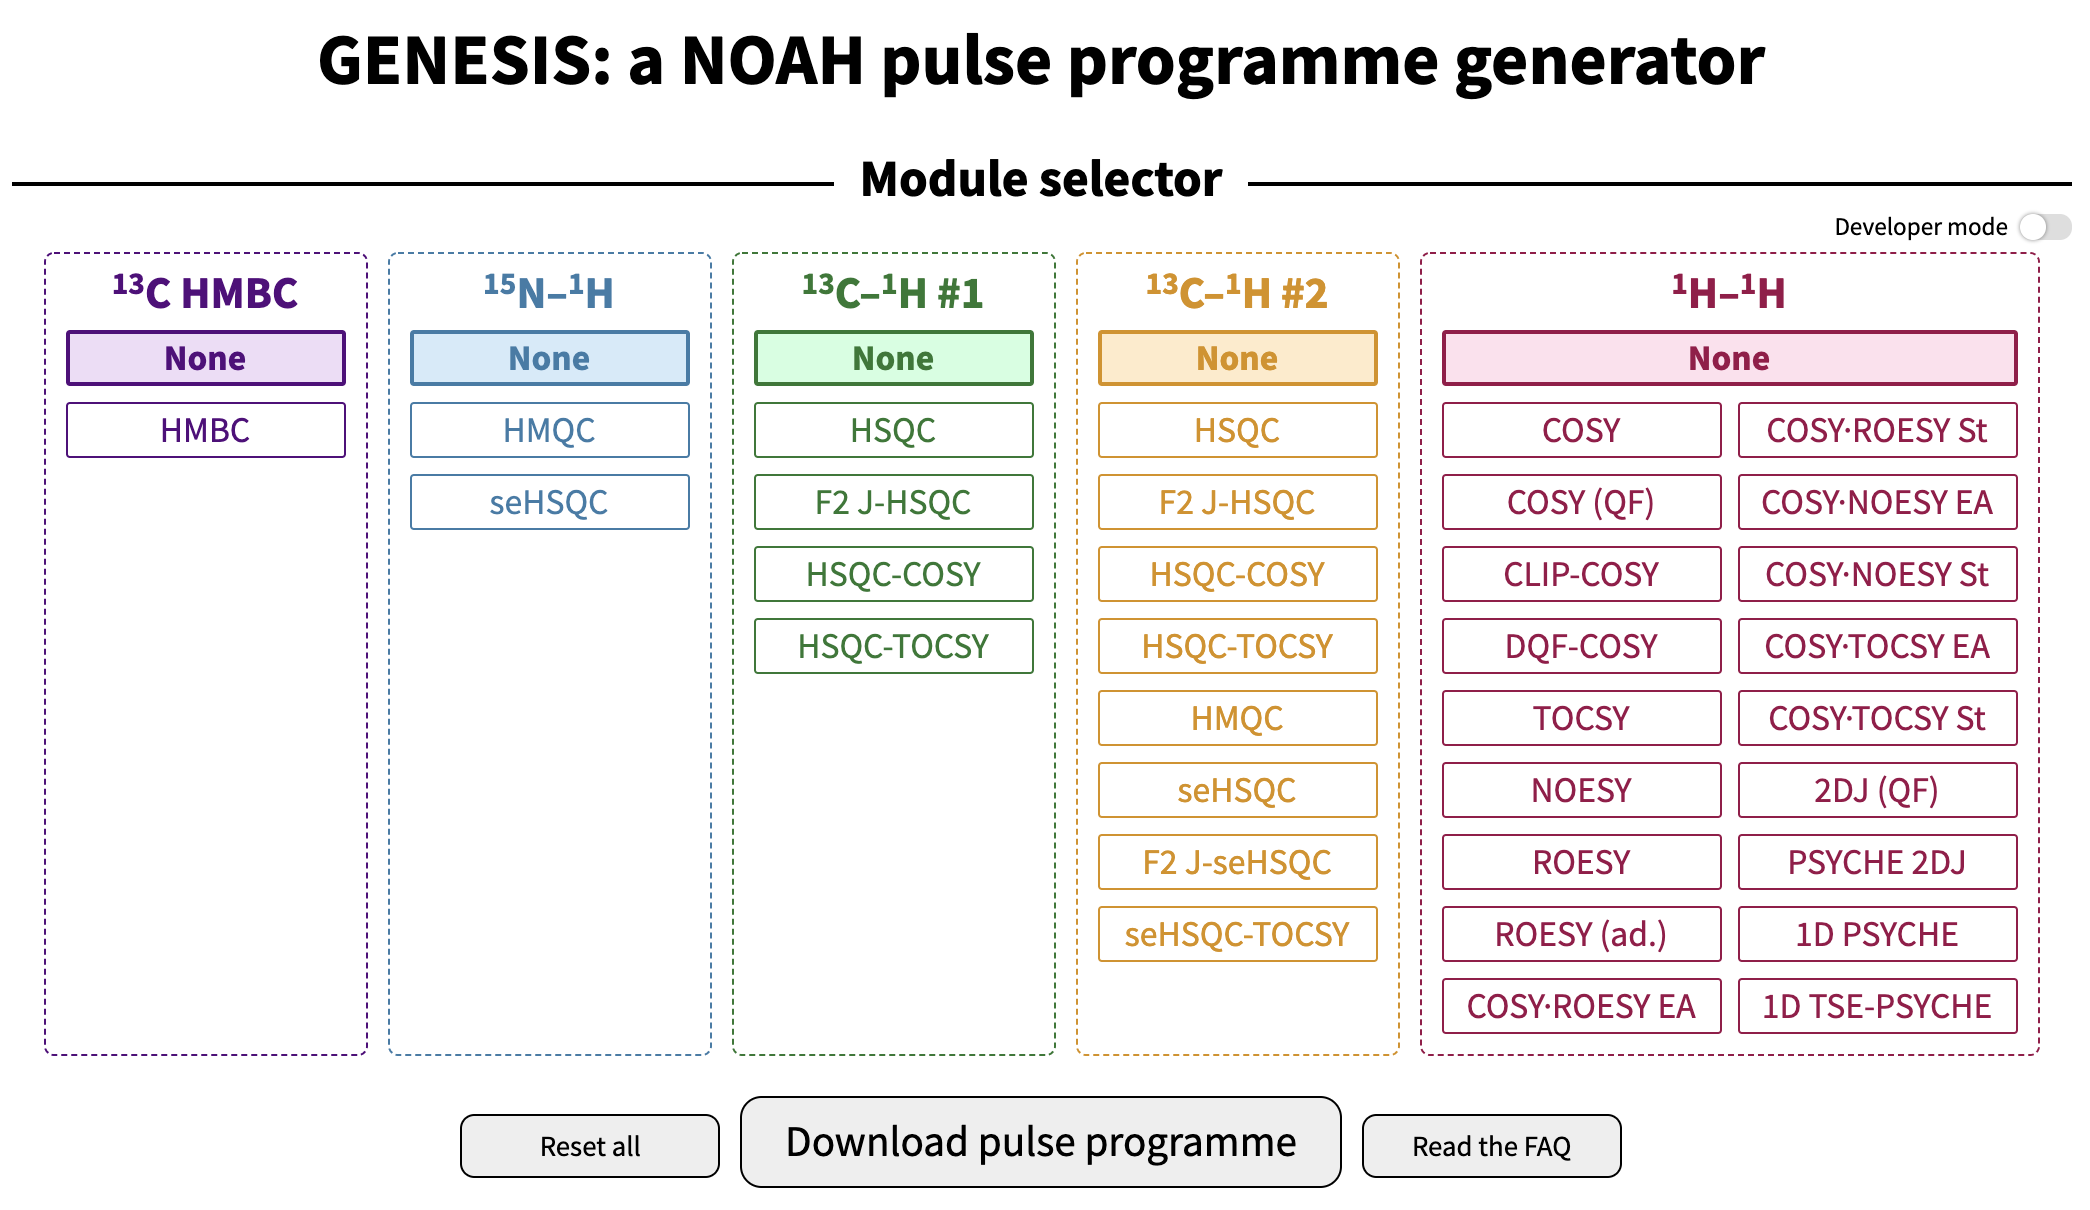
\includegraphics[width=0.6\textwidth]{genesis.png}
    \caption[Short version]{
        What font am I? $y = ax^2 + bx + c$ $M$M
        Lorem ipsum dolor sit amet, consectetur adipiscing elit, sed do eiusmod tempor incididunt ut labore et dolore magna aliqua. Ut enim ad minim veniam, quis nostrud exercitation ullamco laboris nisi ut aliquip ex ea commodo consequat. Duis aute irure dolor in reprehenderit in voluptate velit esse cillum dolore eu fugiat nulla pariatur. Excepteur sint occaecat cupidatat non proident, sunt in culpa qui officia deserunt mollit anim id est laborum.
    }
\end{figure}

\section{Discussion of individual modules}
\label{sec:noah__modules}

The GENESIS website makes it possible to easily implement and distribute entirely new modules, as well as updates to old modules: simply changing the underlying \texttt{NOAHModule} objects is sufficient to propagate changes to all supersequences generated using those modules.
In this section, I discuss a number of new pulse sequence developments made in the course of my DPhil; all of these have been successfully implemented in GENESIS and are available to download.

\subsection{\texorpdfstring{\carbon{}}{13C} sensitivity-enhanced HSQC}
\label{subsec:noah__sehsqc_c}

The first new module is the sensitivity-enhanced HSQC (seHSQC) experiment, which provides up to $2\times$ increased SNR over a standard (echo--antiecho) HSQC.%
\footnote{Since a States HSQC has $\sqrt{2}$ times the SNR of an EA HSQC (as shown in \cref{fig:hsqc_comparison}), this also means that the seHSQC has a $\sqrt{2}$ SNR improvement over a States HSQC. The literature can be somewhat confusing on this point: sometimes the gain in signal is even conflated with the gain in SNR. The clearest exposition I have found is that provided by Kontaxis et al.\autocite{Kontaxis1994JMRSA}}
In the original version of the seHSQC (\cref{fig:sehsqc_po_crk}), developed by Cavanagh, Rance, and Kay (`CRK')\autocite{Palmer1991JMR,Kay1992JACS}, this is accomplished through the so-called \textit{preservation of equivalent pathways} (PEP) technique\autocite{Cavanagh1993ARNMRS}.

\begin{figure}[!htbp]
    \centering
    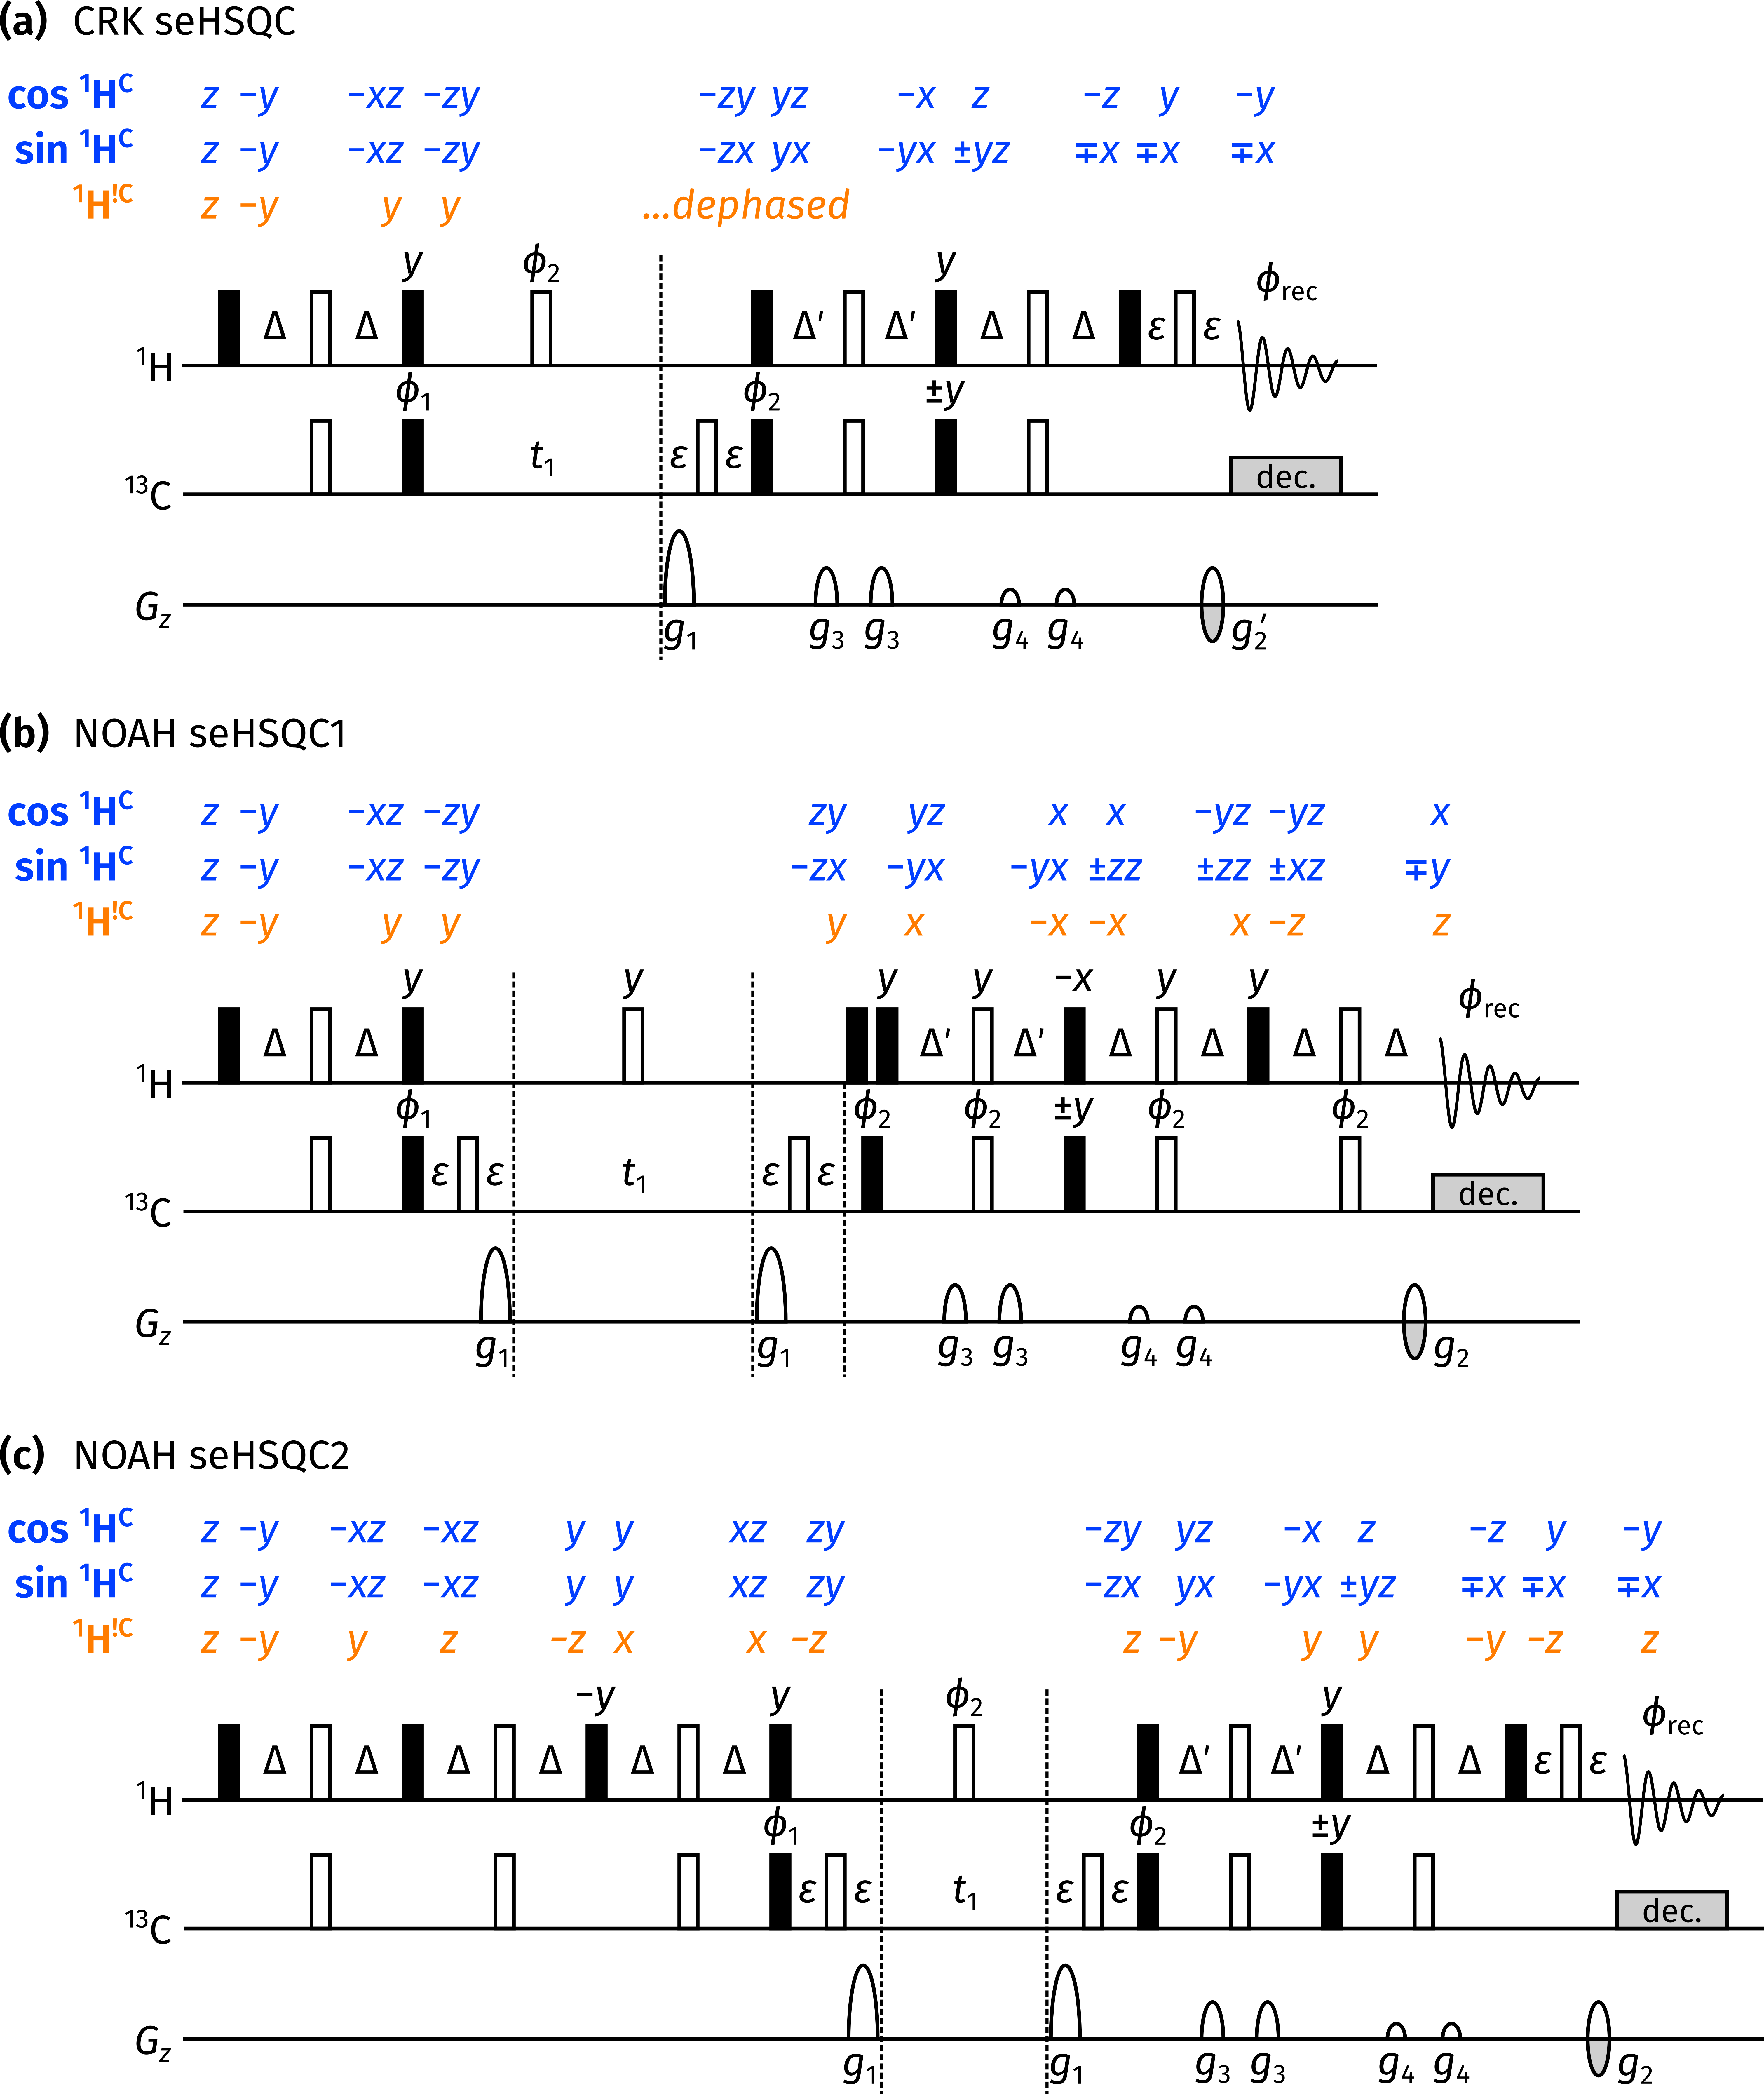
\includegraphics[]{pp/sehsqc/all_po.png}%
    {\phantomsubcaption\label{fig:sehsqc_po_crk}}%
    {\phantomsubcaption\label{fig:sehsqc_po_noah1}}%
    {\phantomsubcaption\label{fig:sehsqc_po_noah2}}%
    \caption[CRK seHSQC and NOAH seHSQC modules]{
        Sensitivity-enhanced HSQC sequences discussed in this section, along with product operator analysis.
        This analysis is provided only for the first step of the phase cycle, and assumes an $IS\/$ spin pair with $\Delta' = 1 / (4 \cdot \oneJ{CH})$.
        `cos \magn{C}' refers to the component of the \magn{C} magnetisation which is cosine-modulated during $t_1$.
        \textbf{(\subref*{fig:sehsqc_po_crk})} Cavanagh--Rance--Kay seHSQC.
        \textbf{(\subref*{fig:sehsqc_po_noah1})} NOAH seHSQC1 module.
        \textbf{(\subref*{fig:sehsqc_po_noah2})} NOAH seHSQC2 module.
        Phase cycling is performed with $\phi_1 = (x, -x)$, $\phi_2 = (x, x, -x, -x)$, and $\phi_\text{rec} = (x, -x, -x, x)$.
        The delay $\Delta$ is set to $1 / (4 \cdot \oneJ{CH})$; see the text for a discussion of $\Delta'$.
        The pulses marked with a phase of $\pm y$ are applied with a phase of $y$ in the echo experiment and $-y$ in the antiecho.
        Gradient amplitudes are $(g_1, g_2, g_2', g_3, g_4) = (80\%, \pm 40.2\%, \pm 20.1\%, 11\%, -5\%)$.
    }
    \label{fig:sehsqc_po}
\end{figure}

Just like in a standard HSQC, the experiment begins with an INEPT block and $t_1$ evolution.
At the end of $t_1$, there are two terms which are cosine- and sine-modulated with respect to $\Omega_S$.
In the standard HSQC, only the $2I_zS_y$ term is returned into observable \proton{} magnetisation by the reverse INEPT block (see \cref{subsec:theory__hsqc_states}).
In contrast, the PEP block transfers \textit{both} terms back to \proton{} and subsequently detects both.
Specifically, in the echo experiment it accomplishes the transfer $2I_zS_y \to I_y$ and $2I_zS_x \to I_x$, meaning that the density operator at the end of $t_1$
\begin{equation}
    \label{eq:sehsqc_t1_modulation}
    -2I_zS_y \cos(\Omega_S t_1) - 2I_zS_x \sin(\Omega_S t_1)
\end{equation}
is transformed into
\begin{equation}
    \label{eq:sehsqc_before_detection}
    -I_y \cos(\Omega_S t_1) - I_x \sin(\Omega_S t_1)
\end{equation}
just prior to acquisition.
During the FID, only the $-1$-coherence component is detected:
\begin{equation}
    \label{eq:sehsqc_detection_minusone}
    \frac{1}{2\mi}I_- \cos(\Omega_S t_1) - \frac{1}{2}I_- \sin(\Omega_S t_1) = \frac{1}{2\mi}I_-\exp(-\mi \Omega_S t_1),
\end{equation}
yielding a signal of
\begin{equation}
    \label{eq:s_echo_sehsqc}
    \frac{1}{2\mi}\exp(-\mi \Omega_S t_1)\exp(\mi \Omega_I t_2),
\end{equation}
which has a $2\times$ larger amplitude than the original EA HSQC (\cref{eq:hsqc_ea_echo_signal}).
The antiecho experiment can be similarly analysed.
Since the seHSQC has the same noise level as in an EA HSQC, this also corresponds to a $2\times$ increase in SNR.

It should, however, be noted that the PEP transfer is only fully attained for $IS\/$ spin pairs if the delay $\Delta'$ is set to $1 / (4 \cdot \oneJ{CH})$.
For $I_2S\/$ or $I_3\/S$ spin systems, no gain in sensitivity is accomplished with this setting of $\Delta' = 1 / (4 \cdot \oneJ{CH})$.
It is more common, therefore, to shorten $\Delta'$ to $1 / (8 \cdot \oneJ{CH})$: this sacrifices some transfer efficiency for $IS\/$ systems, but allows for some sensitivity enhancement for $I_2S\/$ and $I_3S\/$ systems (\cref{tbl:sehsqc_theory}).
In this work, all experiments were run assuming a value of \qty{145}{\Hz} for $\oneJ{CH}$.

\begin{table}[!ht]
    \begin{tabular}{cccc}
        \toprule
        \textbf{Spin system} & \multicolumn{3}{c}{\textbf{Theoretical sensitivity enhancement}} \\
        \cmidrule(lr){2-4}
                             & $\Delta' = 1 / (4 \cdot \oneJ{CH})$ & $\Delta' = 1 / (8 \cdot \oneJ{CH})$ & $\Delta' = 1 / (12 \cdot \oneJ{CH})$ \\
        \midrule
        $IS$   & 2 & 1.71 & 1.5  \\
        $I_2S$ & 1 & 1.41 & 1.37 \\
        $I_3S$ & 1 & 1.21 & 1.25 \\
        \bottomrule
    \end{tabular}
    \caption[Theoretical sensitivity enhancements in the seHSQC]{
        Theoretical sensitivity enhancements for $IS\/$, $I_2S\/$, and $I_3S\/$ spin systems in the seHSQC, as a function of the delay $\Delta'$.
        The values are taken from Schleucher et al.\autocite{Schleucher1994JBNMR}
    }
    \label{tbl:sehsqc_theory}
\end{table}


\subsubsection{NOAH seHSQC versions}

Just like the original EA HSQC (\cref{fig:hsqc_etgp}), the CRK seHSQC must be modified in order to be compatible with NOAH supersequences.
In particular, the CTP gradients in the CRK seHSQC dephase the bulk \magnnot{C} magnetisation pool: we would very much like it to return that to $+z$ instead, so that it can be sampled in later homonuclear modules (or, indeed, a HMBC module).
This experiment is more tricky to adapt than the HSQC, because there are \textit{three} different magnetisation components to juggle: the cosine-modulated \magn{C}, sine-modulated \magn{C}, and \magnnot{C}.
Nevertheless, there are at least two ways of doing so; these two modified modules are labelled seHSQC1 and seHSQC2 respectively.

The seHSQC1 module (\cref{fig:sehsqc_po_noah1}) was developed by me.\footnote{Through a great deal of trial and error, and certainly \textit{not} intelligent design.}
It retains the same general structure of the CRK seHSQC up until $t_1$, but immediately after $t_1$ a composite \proton{} pulse is used to effect the transformations
\begin{equation}
    \label{eq:sehsqc1_dp}
    I_z \to I_y; \qquad I_y \to I_x,
\end{equation}
where the former is required for the \magn{C} pool and the latter for \magnnot{C}.
This has the effect of storing the sine-modulated term as $2I_zS_z$ magnetisation for one spin echo (as opposed to the CRK seHSQC, which stores cosine-modulated term as $I_z$).
At the beginning of the final spin echo (containing the rephasing gradient), this is transformed into antiphase magnetisation of the form $2I_xS_z$; thus, this spin echo must be lengthened to a total duration of $2\Delta$ in order to fully refocus $\oneJ{CH}$.
The final modification involves the addition of an extra gradient immediately before to $t_1$: this ensures that the bulk \magnnot{C} magnetisation is not dephased, just like in the NOAH HSQC module (\cref{fig:noah_sb_po_s}).

The seHSQC2 module (\cref{fig:sehsqc_po_noah2}), on the other hand, was initially reported by Hansen et al.\autocite{Hansen2021AC}
In this pulse sequence, the initial \proton{} \ang{90} excitation pulse is replaced with a $zz$ isotope-selective pulse element (ZIP element), which is very similar to the $zz$-filter but has different pulse phases.
This acts as a 90\rlap{\unit{\degree}}$_{-x}$ pulse on the \magn{C} magnetisation pool and thus ultimately leads to the same signals being detected (save for a trivial \ang{180} phase shift).
However, on \magnnot{C} magnetisation, the ZIP element acts as a 90\rlap{\unit{\degree}}$_{y}$ pulse; it turns out that this modification alone is sufficient to return the bulk \magnnot{C} magnetisation to $+z$ at the end of the sequence.
The ZIP element therefore represents an isotope-specific rotation on \proton{} spins, where the rotation axis depends on whether it is coupled to \carbon{} or not.

\begin{figure}[!ht]
    \centering
    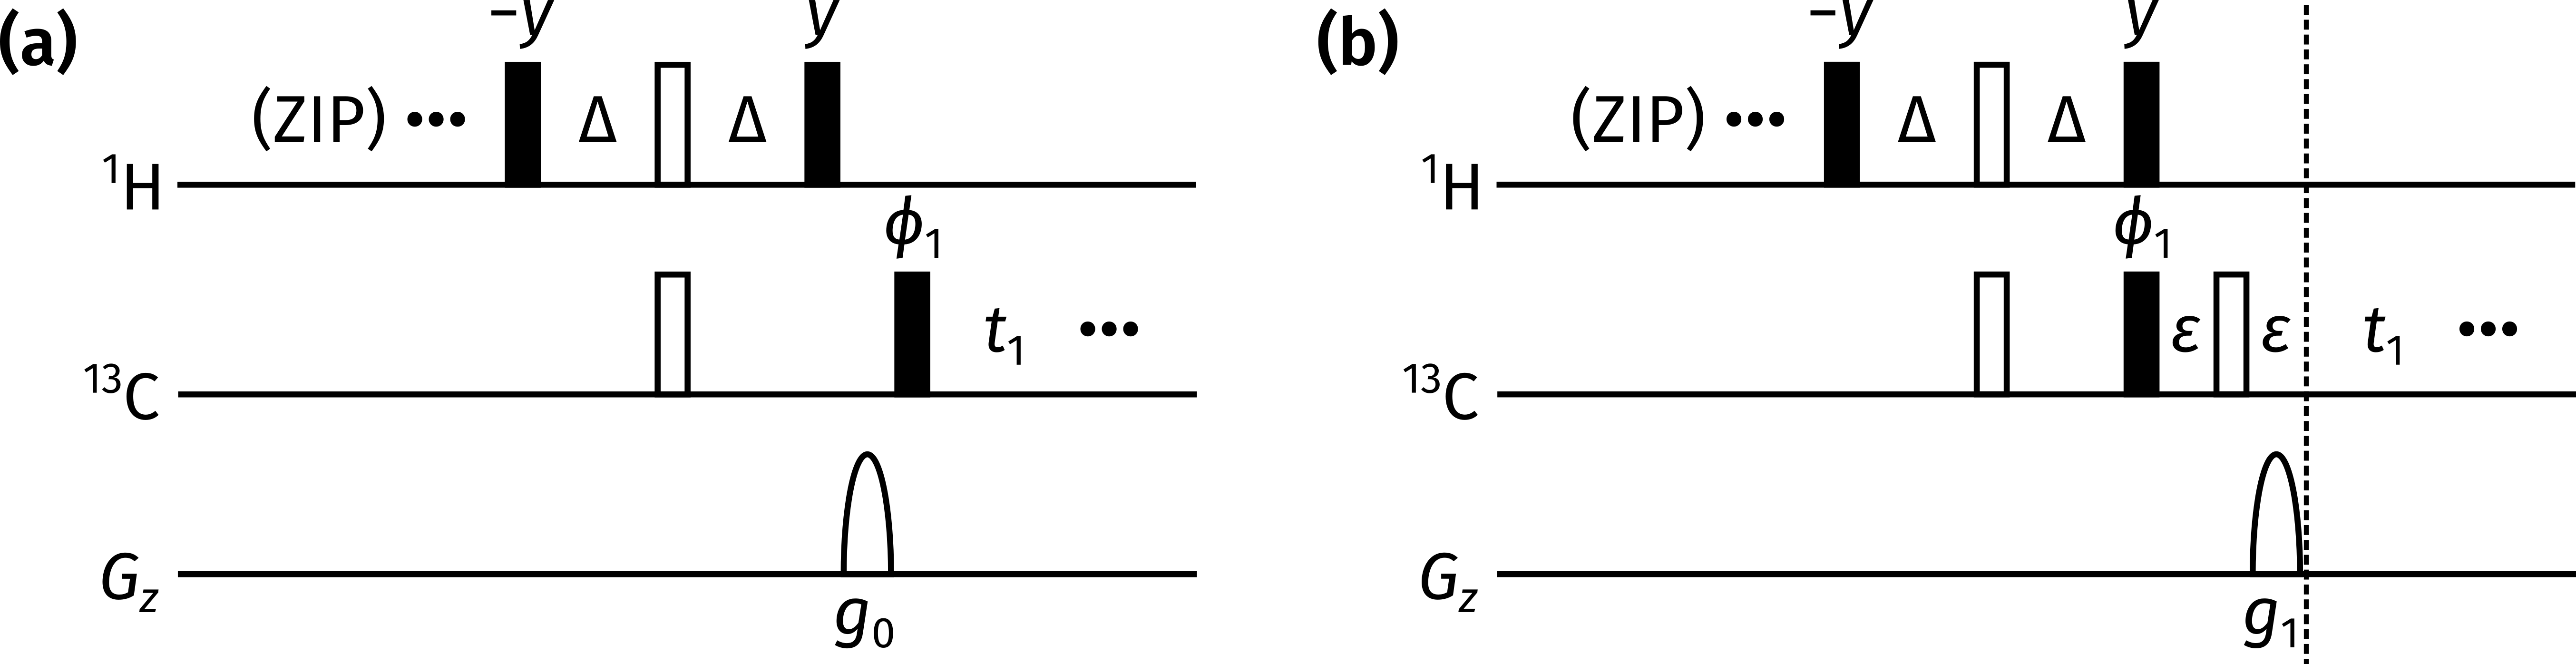
\includegraphics[]{pp/sehsqc/grad_schemes.png}%
    {\phantomsubcaption\label{fig:sehsqc_grad_schemes_alex}}%
    {\phantomsubcaption\label{fig:sehsqc_grad_schemes_jon}}%
    \caption[Comparison of gradient schemes in seHSQC2 module]{
        Comparison of CTP gradient schemes in seHSQC2 module.
        \textbf{(\subref*{fig:sehsqc_grad_schemes_alex})} As reported in Hansen et al.\autocite{Hansen2021AC} $g_0$ is a purge gradient with arbitrary amplitude; the amplitude of the final CTP gradient must be halved.
        \textbf{(\subref*{fig:sehsqc_grad_schemes_jon})} The version used in this work (corresponding to \cref{fig:sehsqc_po_noah2}).
    }
    \label{fig:sehsqc_grad_schemes}
\end{figure}

In my work, I made one change to the experiment, namely the addition of an extra gradient echo prior to $t_1$ (thus leading to a symmetric gradient scheme similar to that in seHSQC1).
Instead of this, the original paper had in fact inserted a purge gradient between the \proton{} and \carbon{} \ang{90} pulses just after the INEPT spin echo (\cref{fig:sehsqc_grad_schemes}).
The scheme I used leads to similar results, but has one advantage in that it allows the amplitude of the final CTP gradient ($g_2$ in \cref{fig:sehsqc_po}) to be twice as large: this is particularly relevant to \nitrogen{} experiments, as will be discussed in \cref{subsec:noah__hmqc}.

\begin{figure}[!ht]
    \centering
    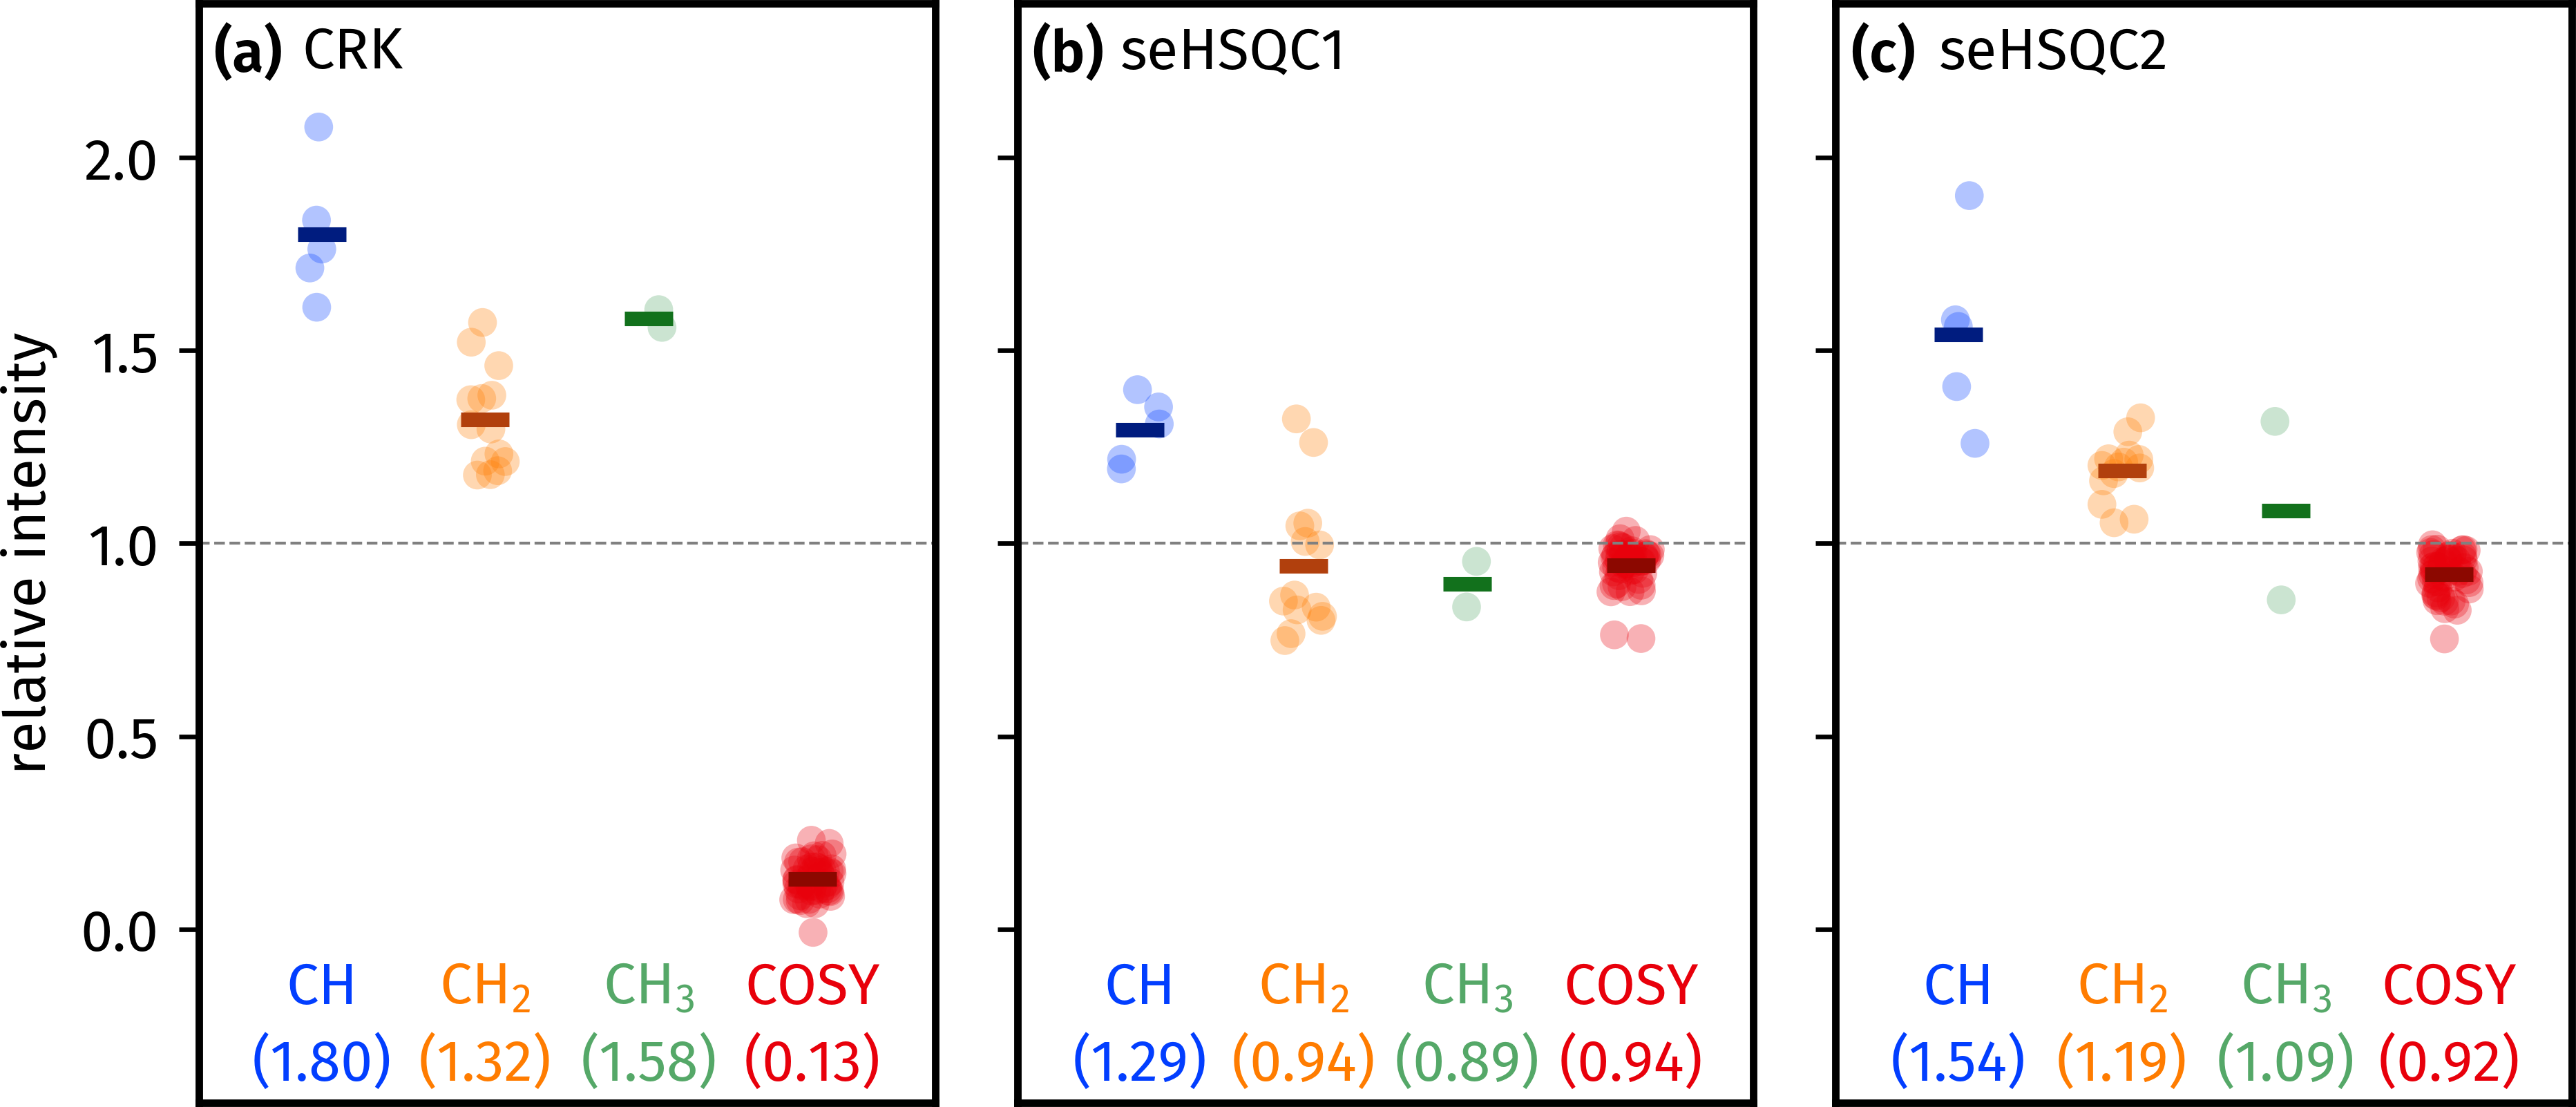
\includegraphics[]{noah/sehsqc_comp.png}%
    {\phantomsubcaption\label{fig:noah_sehsqc_comp_crk}}%
    {\phantomsubcaption\label{fig:noah_sehsqc_comp_v1}}%
    {\phantomsubcaption\label{fig:noah_sehsqc_comp_v2}}%
    \caption[Comparison of \noah{Sp,Cc} sensitivities]{
        Sensitivities of seHSQC and CLIP-COSY modules in the \noah{Sp,Cc} supersequences (run using $\Delta' = 1 / (8 \cdot \oneJ{CH})$).
        Intensities are reported relative to the corresponding peaks in a \noah{S,Cc} supersequence; HSQC peaks are further broken down by their multiplicity.
        Each dot represents one peak; the solid lines as well as the numbers at the bottom of each plot represent averages over all peaks.
        \textbf{(\subref*{fig:noah_sehsqc_comp_crk})} Using the CRK seHSQC.
        \textbf{(\subref*{fig:noah_sehsqc_comp_v1})} Using the seHSQC1 module.
        \textbf{(\subref*{fig:noah_sehsqc_comp_v2})} Using the seHSQC2 module.
        \datacode{7A-201115}
    }
    \label{fig:noah_sehsqc_comp}
\end{figure}

The primary consideration when evaluating the different seHSQC versions in \cref{fig:sehsqc_po} is naturally sensitivity
\Cref{fig:noah_sehsqc_comp} compares the sensitivities of the various possible \noah{Sp,Cc} supersequence against a \noah{S,Cc} experiment.
As can be seen, all three seHSQC implementations yield improvements in the sensitivities of \ch{CH} peaks: the original CRK seHSQC has the largest effect here, followed by seHSQC2 and seHSQC1.
For \ch{CH2} and \ch{CH3} peaks, the CRK seHSQC and seHSQC2 perform better than the standard HSQC, but the average sensitivities in seHSQC1 have dipped slightly below.
This is not entirely surprising in light of the discussion in \cref{subsec:noah__snr}: the modified seHSQC1 and seHSQC2 sequences are expected to have lower sensitivities than the original experiment from which they are derived.
In this case, it appears that the modifications made to the seHSQC1 sequence have caused sensitivity losses which outweigh the benefits of using a sensitivity-enhanced experiment.

In the context of a NOAH supersequence, it is also important to consider how well each module preserves \magnnot{C} magnetisation for subsequent homonuclear module(s).
In \cref{fig:noah_sehsqc_comp}, the CLIP-COSY module is used as the `reporter' module, but the conclusions drawn here are applicable to \textit{any} homonuclear module (or HMBC).
The CRK seHSQC naturally does poorly in this respect, as it dephases the bulk magnetisation: this leads to almost an order-of-magnitude sensitivity loss in the CLIP-COSY.
Both the other NOAH seHSQC modules, however, perform almost identically to the original HSQC module, as expected from the product operator analysis in \cref{fig:sehsqc_po}.

From \cref{fig:noah_sehsqc_comp}, we can draw some very simple conclusions: if the seHSQC is to be used at (or near) the \textit{beginning} of a NOAH supersequence, where it needs to preserve \magnnot{C} magnetisation, then the seHSQC2 module is the best choice.
On the other hand, if the seHSQC module is placed at the \textit{end} (say in a \noah{B,Sp} supersequence), then the CRK seHSQC is optimal.
This logic is encoded in GENESIS.


\subsubsection{COSY-type artefacts}

One (minor) way in which the seHSQC1 module outperforms seHSQC2 is in the suppression of COSY-type artefacts in the seHSQC spectrum\autocite{Turner1999JMR}.
These arise due to evolution of $\nJ{HH}$ during the second-last spin echo of the CRK seHSQC.
Specifically, if we assume the presence of a separate \proton{} spin $K$ which is coupled to spin $I$, the sine-modulated $2I_yS_z$ term can evolve under both $\oneJ{$IS$}$ and $\nJ{$IK$}$ into $2I_yK_z$, and the last \proton{} \ang{90} pulse transfers this coherence to the spin $K$.
This leads to peaks correlating spin $S$ with $K$.
This is also true of the seHSQC2 module, as the product operator analysis for the CRK seHSQC is entirely applicable to it.

However, for the seHSQC1 module, the corresponding term giving rise to these artefacts would be the cosine-modulated $I_x$ term (at the beginning of the second-last spin echo).
During this spin echo, this can again evolve under both J-couplings into $4I_yK_zS_z$, and the final \ang{90} pulse would transform this to $-4I_zK_yS_z$.
However, crucially, this term is antiphase with respect to the heteronucleus $S$: therefore, when decoupling is applied during acquisition, this term should not be observed.
This analysis can be verified experimentally by inspection of the seHSQC spectra thus obtained.
The COSY-type artefacts, labelled with red boxes in the seHSQC2 spectrum (\cref{fig:sehsqc_cosy_arts_2}), are largely absent in the seHSQC1 spectrum (\cref{fig:sehsqc_cosy_arts_1}).
Some artefacts still remain, which perhaps arise due to pulse imperfections (or perhaps more complicated spin systems than the three-spin system considered here; I did not analyse this in any further detail).

\begin{figure}[!ht]
    \centering
    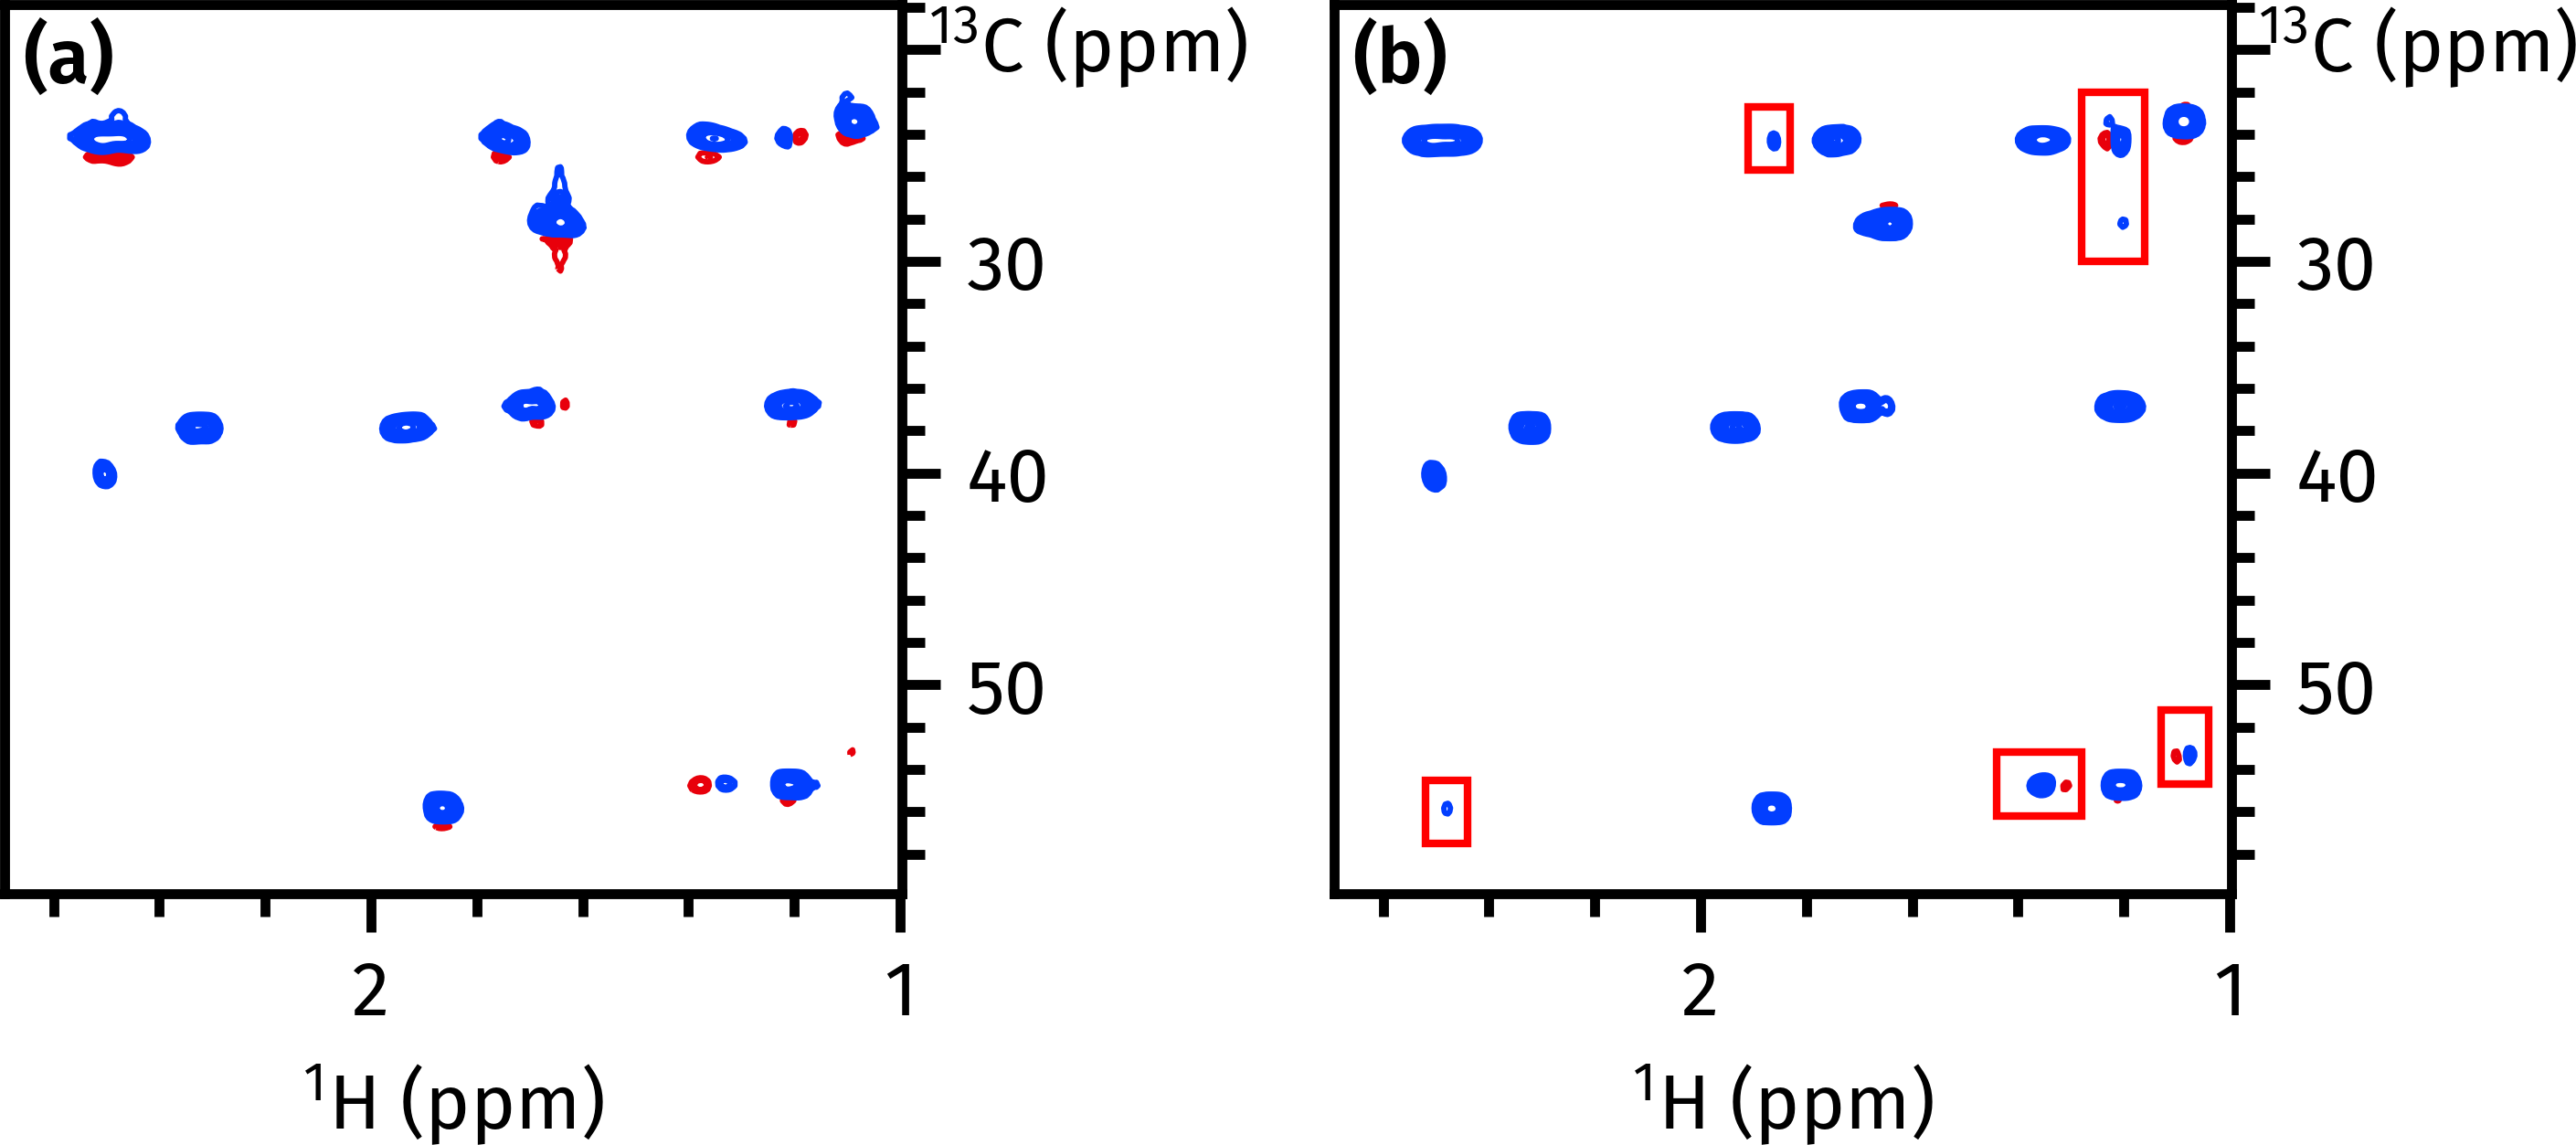
\includegraphics[]{noah/sehsqc_cosy_arts.png}%
    {\phantomsubcaption\label{fig:sehsqc_cosy_arts_1}}%
    {\phantomsubcaption\label{fig:sehsqc_cosy_arts_2}}%
    \caption[Comparison of COSY-type artefacts in NOAH seHSQC modules]{
        Comparison of COSY-type artefacts in NOAH seHSQC modules.
        \textbf{(\subref*{fig:sehsqc_cosy_arts_1})} seHSQC1.
        \textbf{(\subref*{fig:sehsqc_cosy_arts_2})} seHSQC2. The artefacts are highlighted in red boxes.
        \datacode{7A-201115}
    }
    \label{fig:sehsqc_cosy_arts}
\end{figure}


\subsubsection{Wing artefacts}

One point worth considering is whether the extra gradient in the seHSQC2 module is truly needed.
In the HSQC and seHSQC1 modules, the bulk magnetisation is placed along the transverse axis during $t_1$; therefore, if a pair of symmetric gradients are not used, this magnetisation will be dephased (as in the CRK seHSQC).
However, in the seHSQC2 module, the bulk magnetisation is longitudinal, which suggests that this gradient is not necessary.

This gradient can indeed be removed in the seHSQC2 module, and doing so does not lead to any poorer preservation of \magnnot{C} magnetisation.
However, the omission of this gradient leads to artefacts in the CLIP-COSY spectrum, which I term \textit{`wing artefacts'} because of the way they flank peaks in the CLIP-COSY (\cref{fig:sehsqc_wing_arts}).
These artefacts can most clearly be seen in the diagonal peaks of methyl groups, but are present across the entire spectrum.

\begin{figure}[!ht]
    \centering
    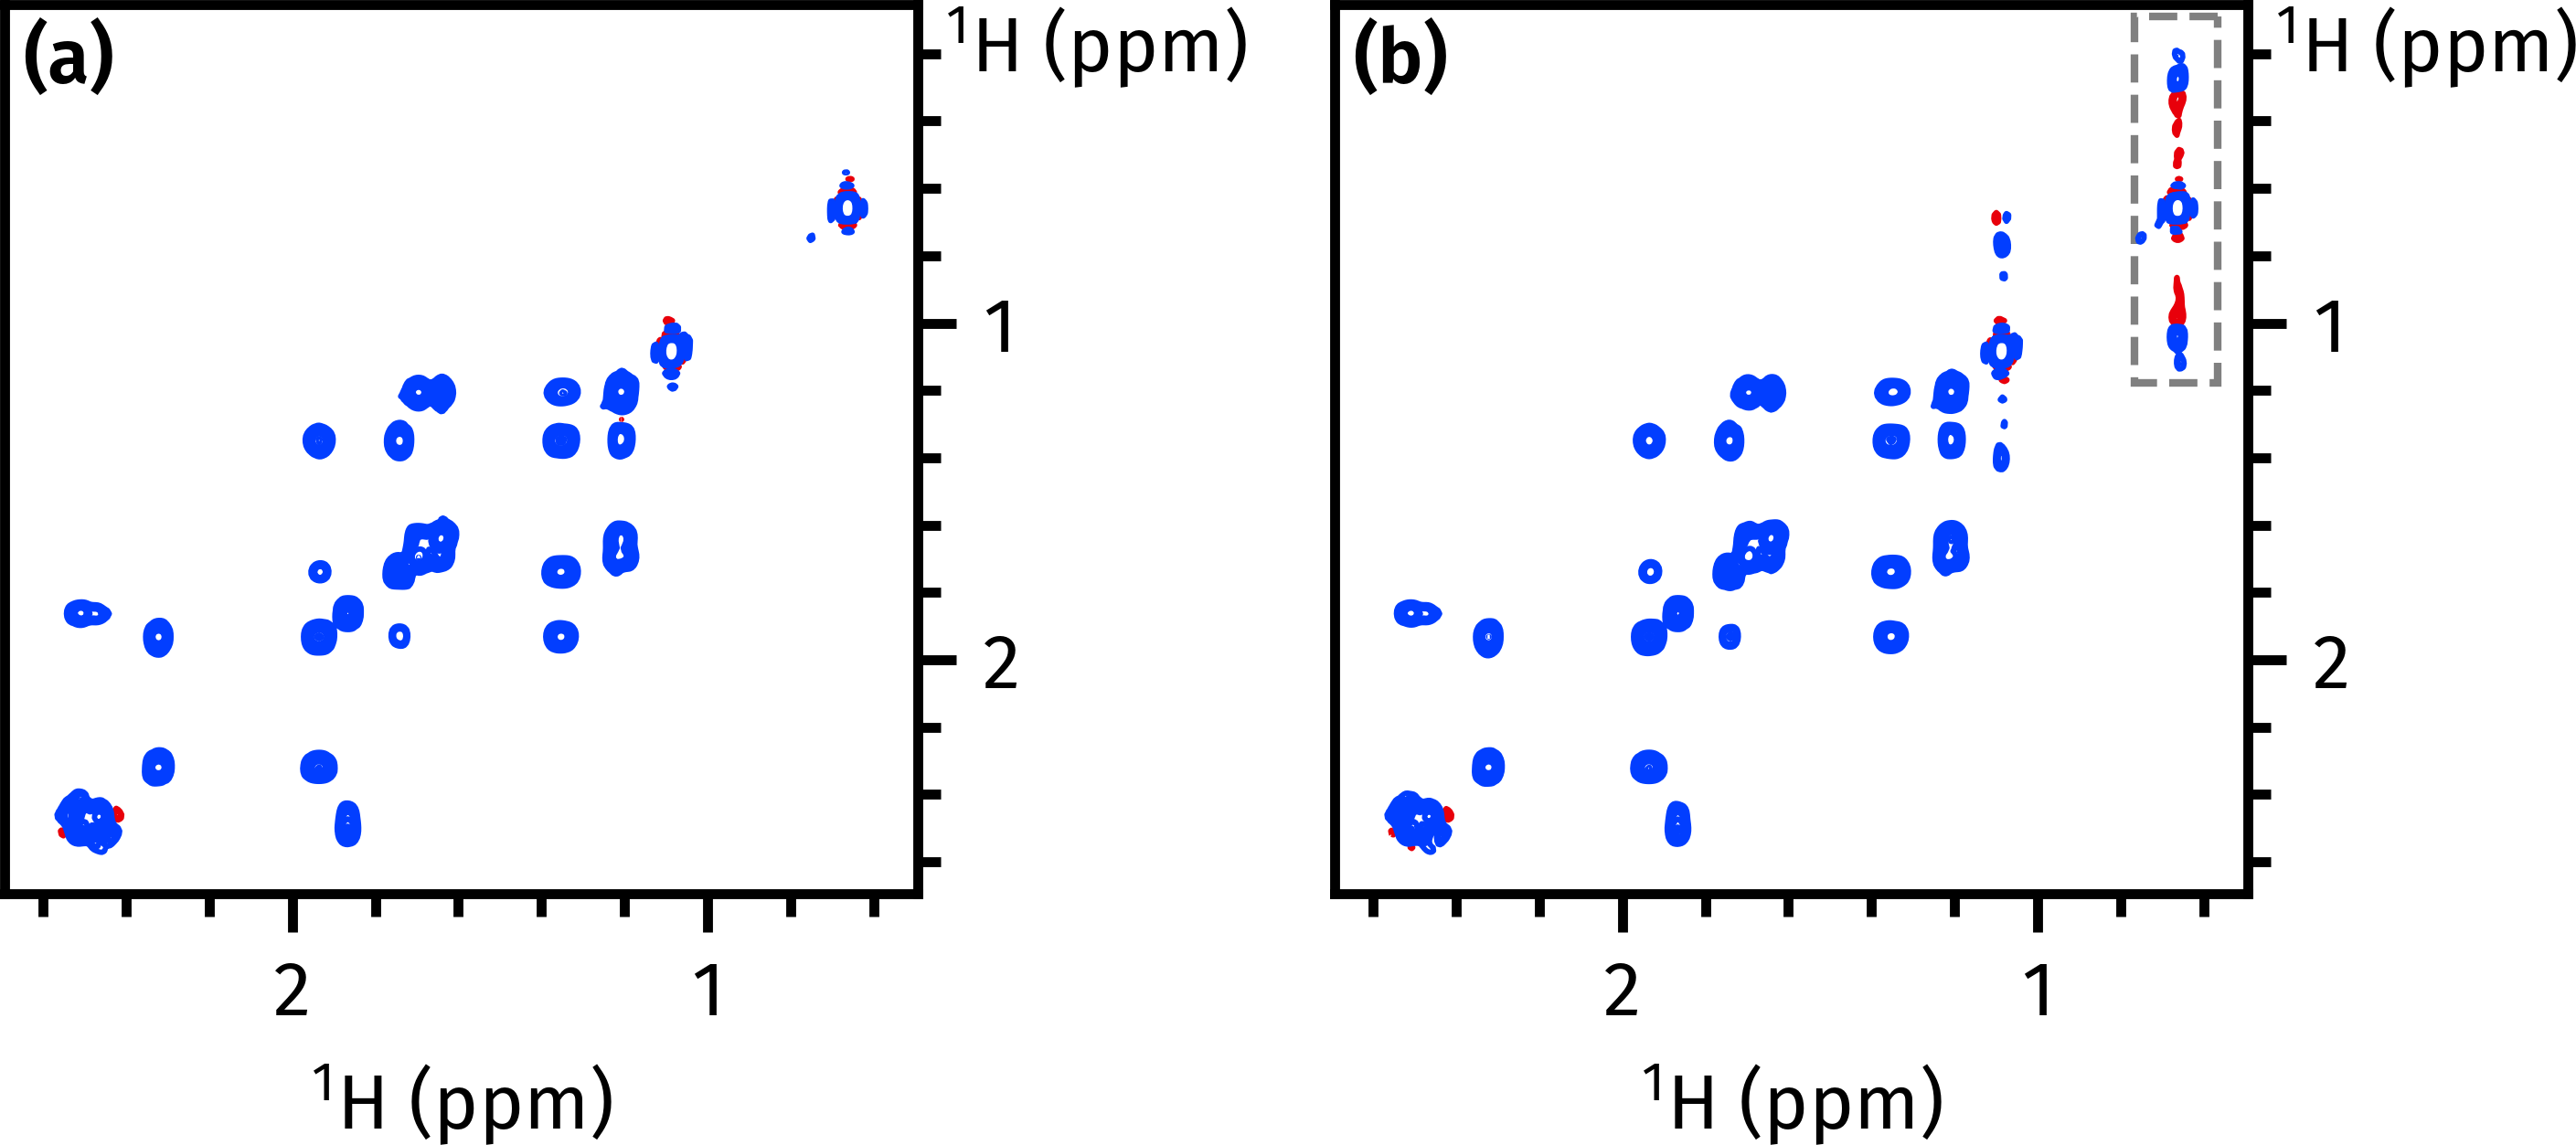
\includegraphics[]{noah/sehsqc_wing_arts.png}%
    {\phantomsubcaption\label{fig:sehsqc_wing_arts_2grad}}%
    {\phantomsubcaption\label{fig:sehsqc_wing_arts_1grad}}%
    \caption[Wing artefacts in CLIP-COSY spectra when extra seHSQC2 gradient is omitted]{
        Wing artefacts in CLIP-COSY spectra, taken from \noah{Sp,Cc} supersequences.
        \textbf{(\subref*{fig:sehsqc_wing_arts_2grad})} Using the seHSQC2 module as shown in \cref{fig:sehsqc_po_noah2}.
        \textbf{(\subref*{fig:sehsqc_wing_arts_1grad})} Using a modified seHSQC2 module where the gradient echo just before $t_1$ is removed.
        The wing artefacts flanking the two rightmost diagonal peaks can be clearly seen; the boxed artefacts are studied further in \cref{fig:sehsqc_wing_arts_proj}.
        \datacode{7A-201115}
    }
    \label{fig:sehsqc_wing_arts}
\end{figure}

A clue as to their origin is provided by the characteristic frequencies of the artefacts:
\begin{equation}
    \label{eq:wing_artefact_frequencies}
    \left(\Omega_1, \Omega_2 = \Omega_I \pm \frac{\Omega_I \cdot [t_{1,\text{HSQC}}/2]}{t_{1,\text{COSY}}}, \Omega_I\right)
\end{equation}
where $t_{1,\text{X}}$ refers to the value of $t_1$ in experiment X (it does not matter which increment is used, because the ratio of $t_1$ in the fraction above is constant).
In accordance with this, when the seHSQC indirect-dimension spectral width is reduced, the artefacts are displaced outwards (\cref{fig:sehsqc_wing_arts_proj_offon_sw4}).
This suggests that these artefacts arise from \magnnot{C} magnetisation which is frequency-labelled in two different $t_1$ periods: specifically, it evolves once during \textit{half} of the seHSQC $t_1$ period, and then again during the CLIP-COSY $t_1$ period.
In fact, it is necessary to apply CTP gradients on both sides of $t_1$ in order to suppress evolution of this stray magnetisation during both halves: if either or both of the gradients are removed, the artefacts are present (\cref{fig:sehsqc_wing_arts_proj_onon,fig:sehsqc_wing_arts_proj_offon,fig:sehsqc_wing_arts_proj_onoff,fig:sehsqc_wing_arts_proj_offoff}).

\begin{figure}[!ht]
    \centering
    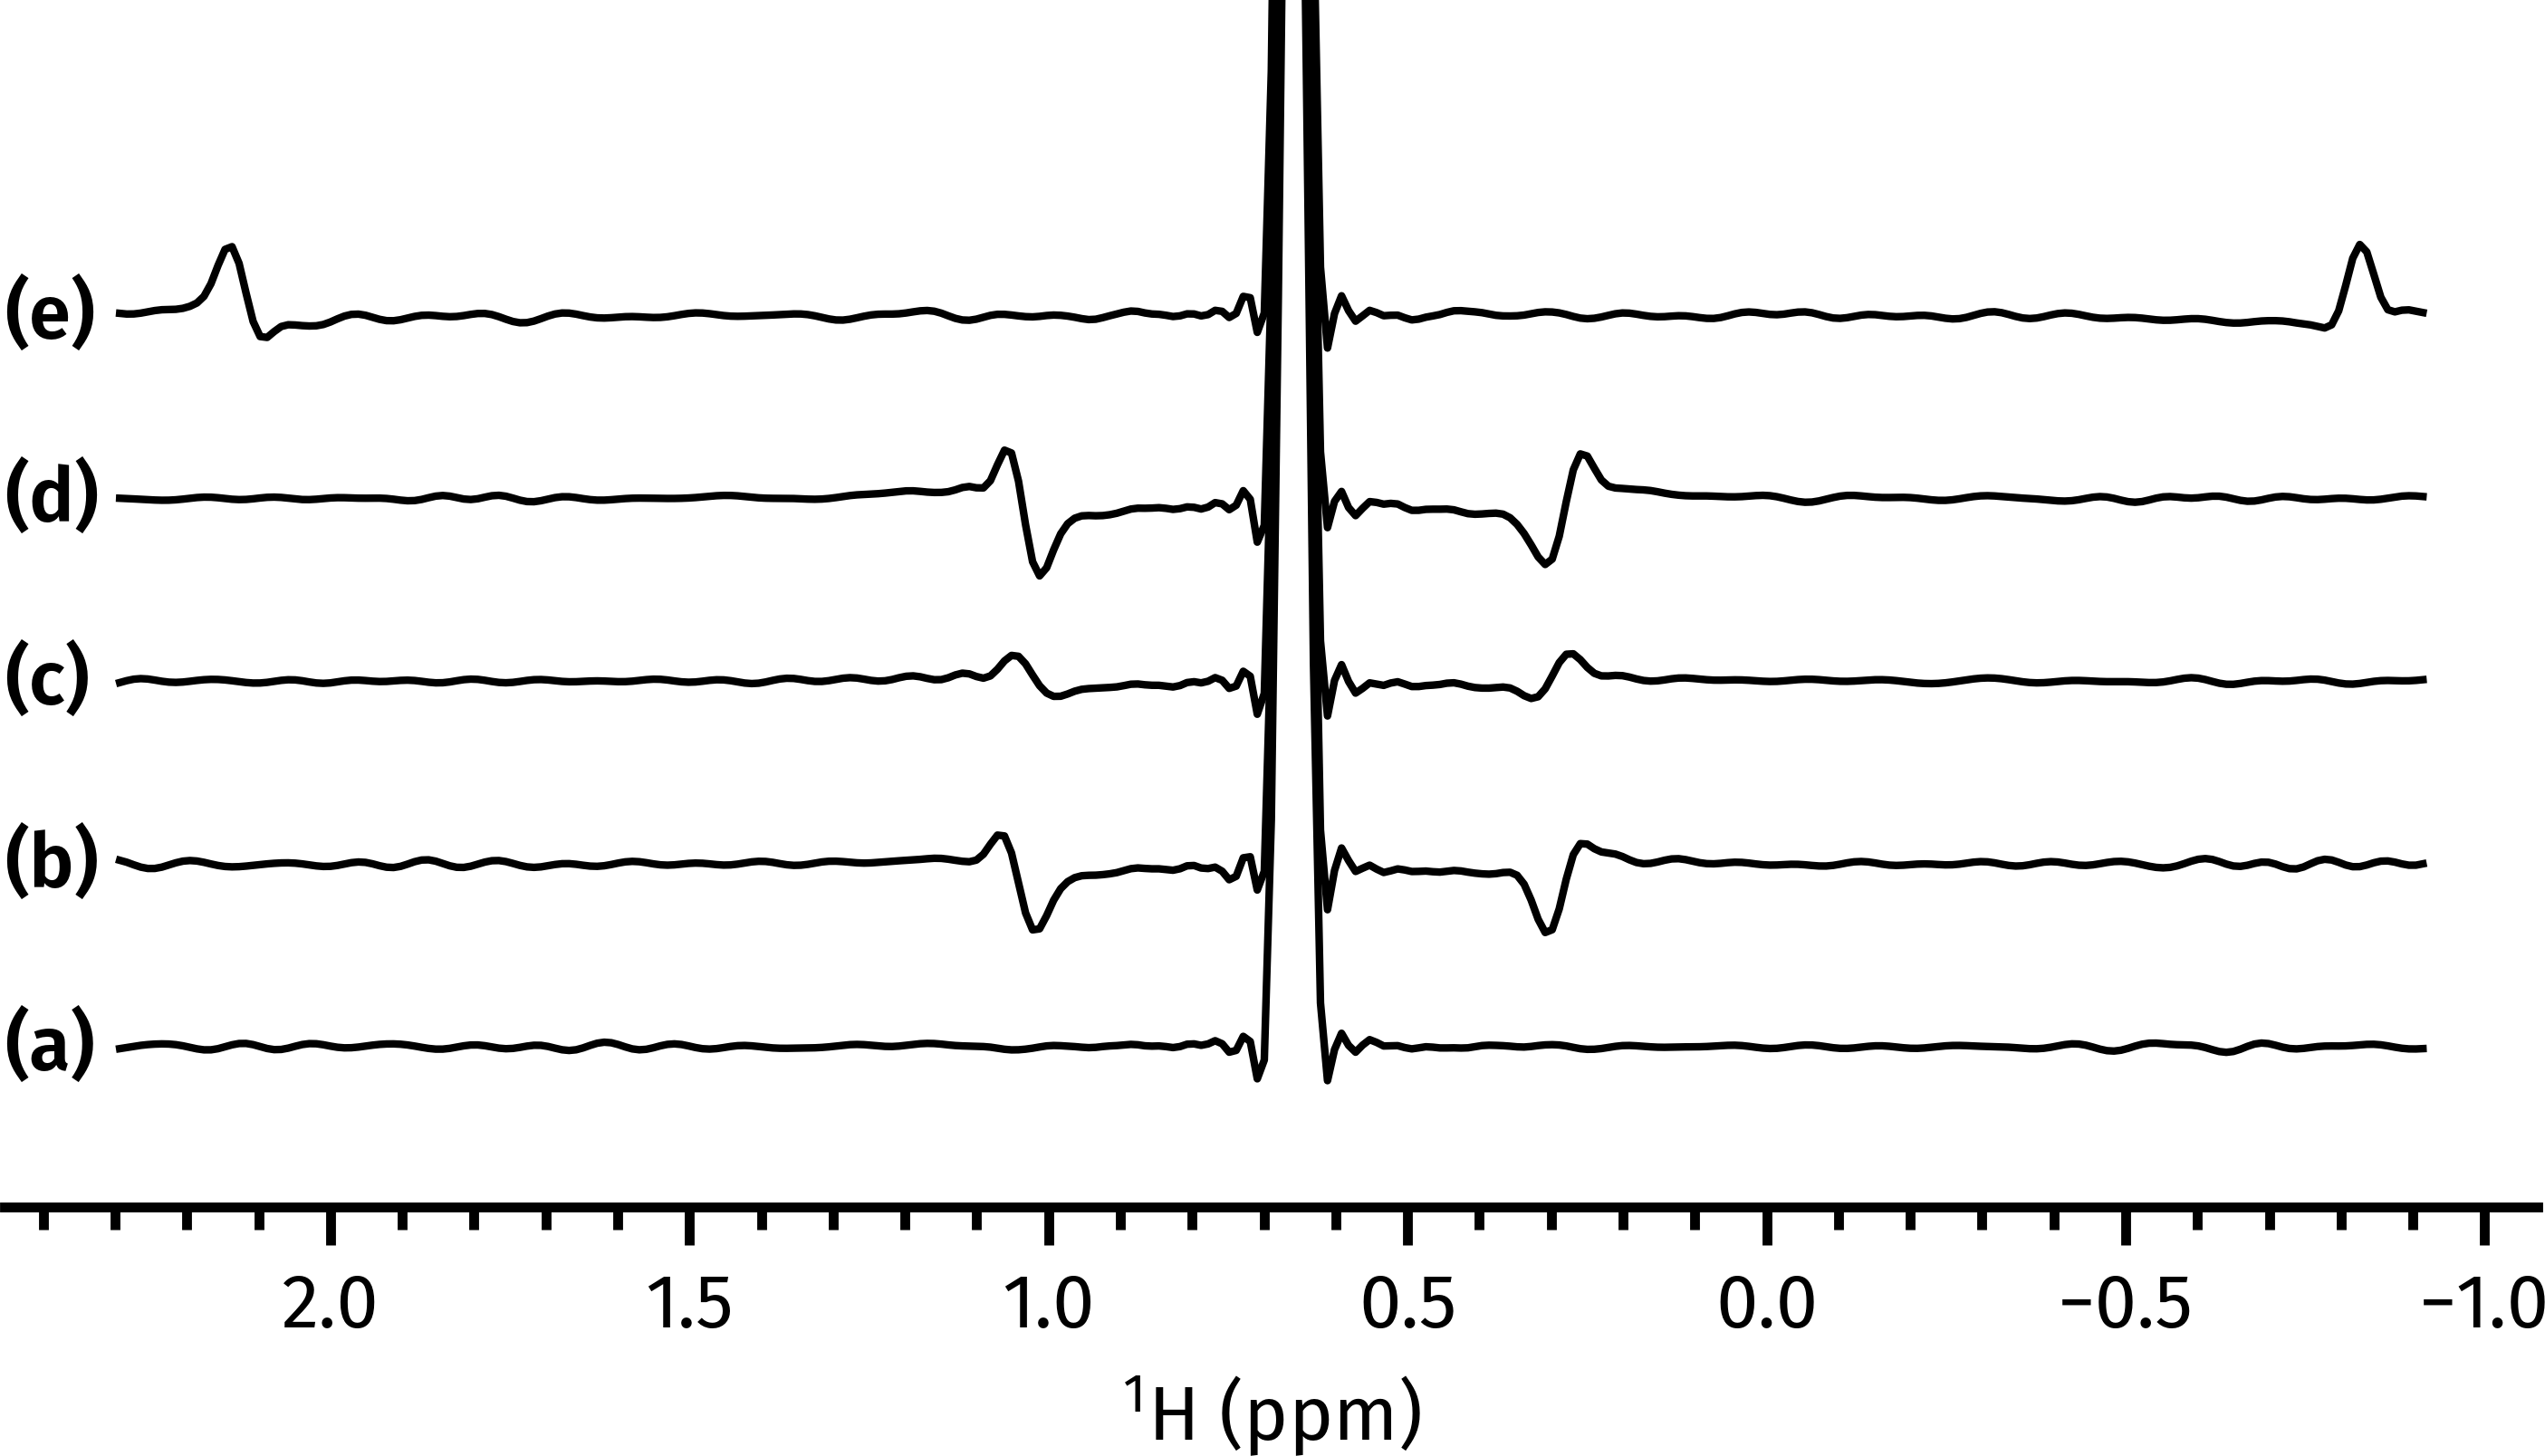
\includegraphics[]{noah/sehsqc_wing_arts_proj.png}%
    {\phantomsubcaption\label{fig:sehsqc_wing_arts_proj_onon}}%
    {\phantomsubcaption\label{fig:sehsqc_wing_arts_proj_offon}}%
    {\phantomsubcaption\label{fig:sehsqc_wing_arts_proj_onoff}}%
    {\phantomsubcaption\label{fig:sehsqc_wing_arts_proj_offoff}}%
    {\phantomsubcaption\label{fig:sehsqc_wing_arts_proj_offon_sw4}}%
    \caption[More detail about wing artefacts in CLIP-COSY spectra]{
        A closer look at wing artefacts in CLIP-COSY spectra, taken from \noah{Sp,Cc} supersequences with various modifications made to the seHSQC2 module.
        The spectra being plotted are 1D slices through $F_2 = \qty{0.67}{\ppm}$ of the 2D CLIP-COSY spectrum; this corresponds to the boxed region in \cref{fig:sehsqc_wing_arts_1grad}.
        \textbf{(\subref*{fig:sehsqc_wing_arts_proj_onon})} Using the default seHSQC2 module, with one gradient before and one after $t_1$.
        \textbf{(\subref*{fig:sehsqc_wing_arts_proj_offon})} The same as (\subref*{fig:sehsqc_wing_arts_proj_onon}), but with the gradient before $t_1$ turned off (the spin echo is still present, but the gradient intensity is set to 0).
        \textbf{(\subref*{fig:sehsqc_wing_arts_proj_onoff})} The same as (\subref*{fig:sehsqc_wing_arts_proj_onon}), but with the gradient after $t_1$ turned off.
        \textbf{(\subref*{fig:sehsqc_wing_arts_proj_offoff})} The same as (\subref*{fig:sehsqc_wing_arts_proj_onon}), but with both gradients turned off.
        \textbf{(\subref*{fig:sehsqc_wing_arts_proj_offon_sw4})} The same as (\subref*{fig:sehsqc_wing_arts_proj_offon}), but with the seHSQC spectral width reduced by a factor of 4.
        \datacode{7A-201115}
    }
    \label{fig:sehsqc_wing_arts_proj}
\end{figure}

These wing artefacts are unique to fast-pulsing experiments such as NOAH supersequences: in a typical 2D experiment, these are less likely to arise because of the long(er) recovery delays between data acquisition periods.
In the sections which follow, we will see these surface repeatedly.
Fortunately, it proves to be relatively easy to suppress them through the judicious use of gradients.


\subsubsection{Multiplicity editing}

Multiplicity editing is reasonably easy to include in all of the seHSQC sequences above.
It suffices to add a spin echo of total duration $4\Delta = 1 / \oneJ{CH}$ just after $t_1$, while also making sure to change some pulse phases to account for the extra \proton{} \ang{180} pulse (\cref{fig:sehsqc_edited}).

\begin{figure}[!ht]
    \centering
    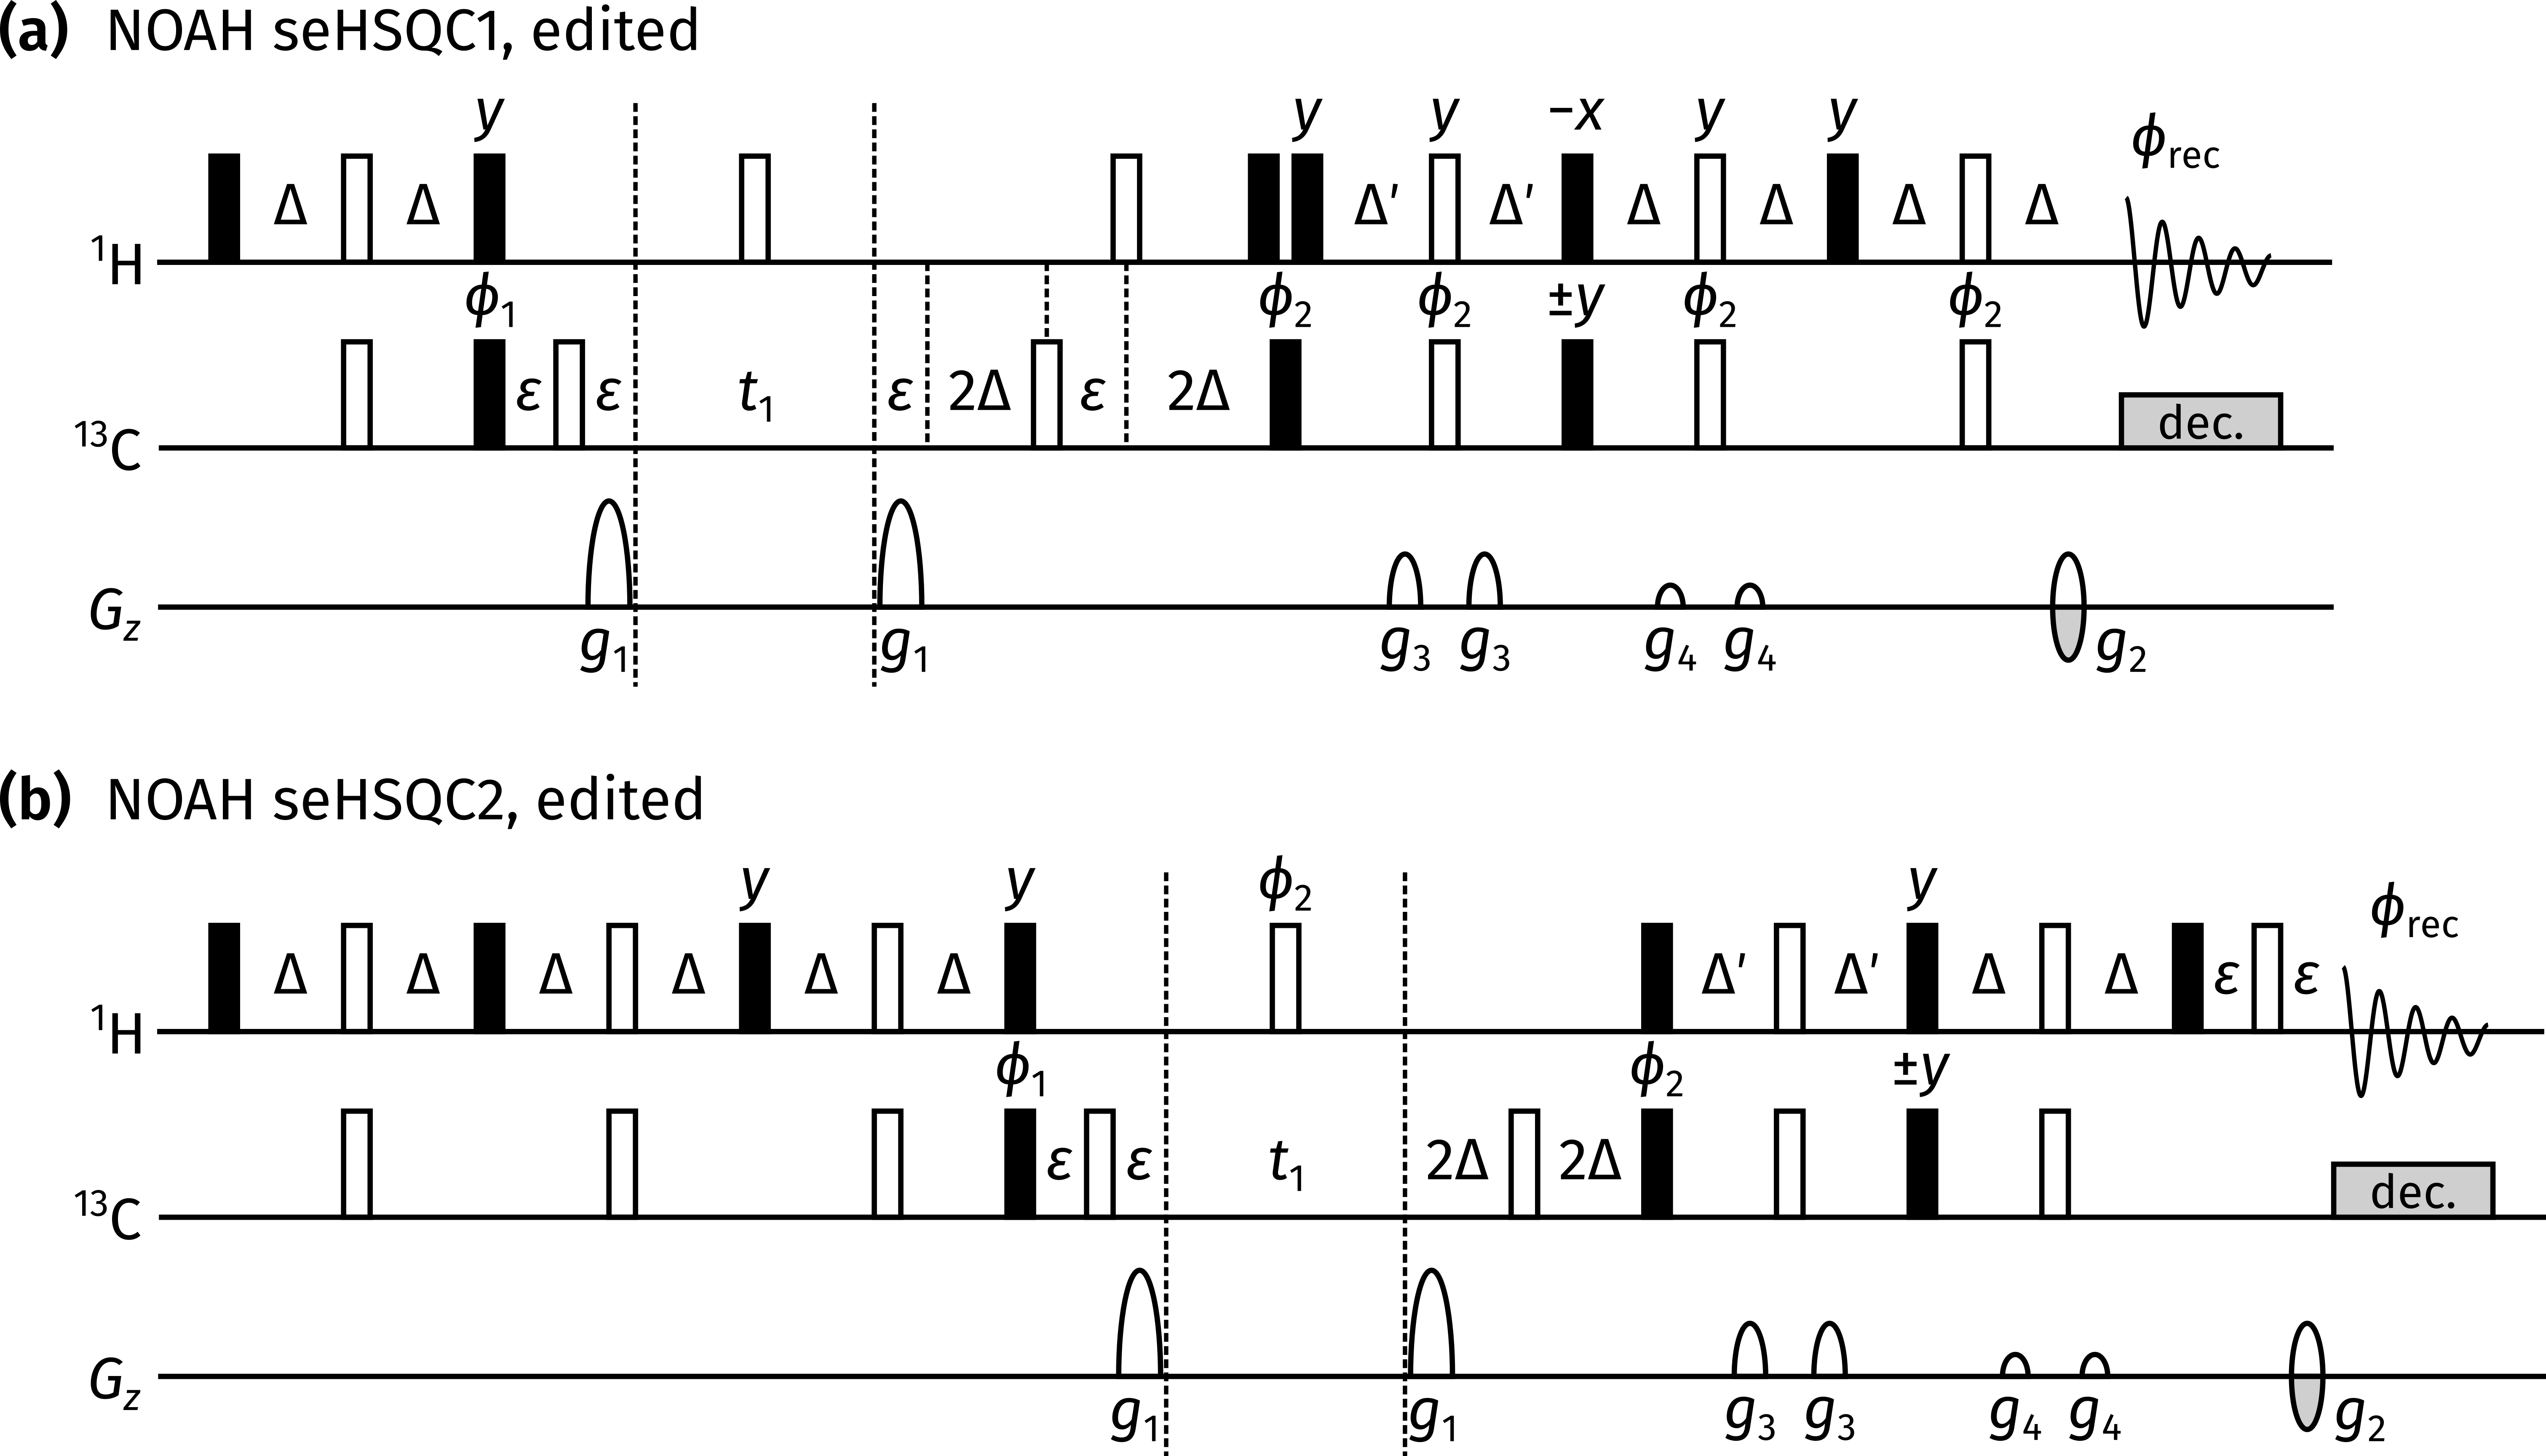
\includegraphics[]{pp/sehsqc/all_edited.png}%
    {\phantomsubcaption\label{fig:sehsqc_edited_1}}%
    {\phantomsubcaption\label{fig:sehsqc_edited_2}}%
    \caption[Multiplicity-edited NOAH seHSQC modules]{
        Multiplicity-edited NOAH seHSQC modules.
        \textbf{(\subref*{fig:sehsqc_edited_1})} Edited seHSQC1.
        \textbf{(\subref*{fig:sehsqc_edited_2})} Edited seHSQC2.
    }
    \label{fig:sehsqc_edited}
\end{figure}

\begin{figure}[!ht]
    \centering
    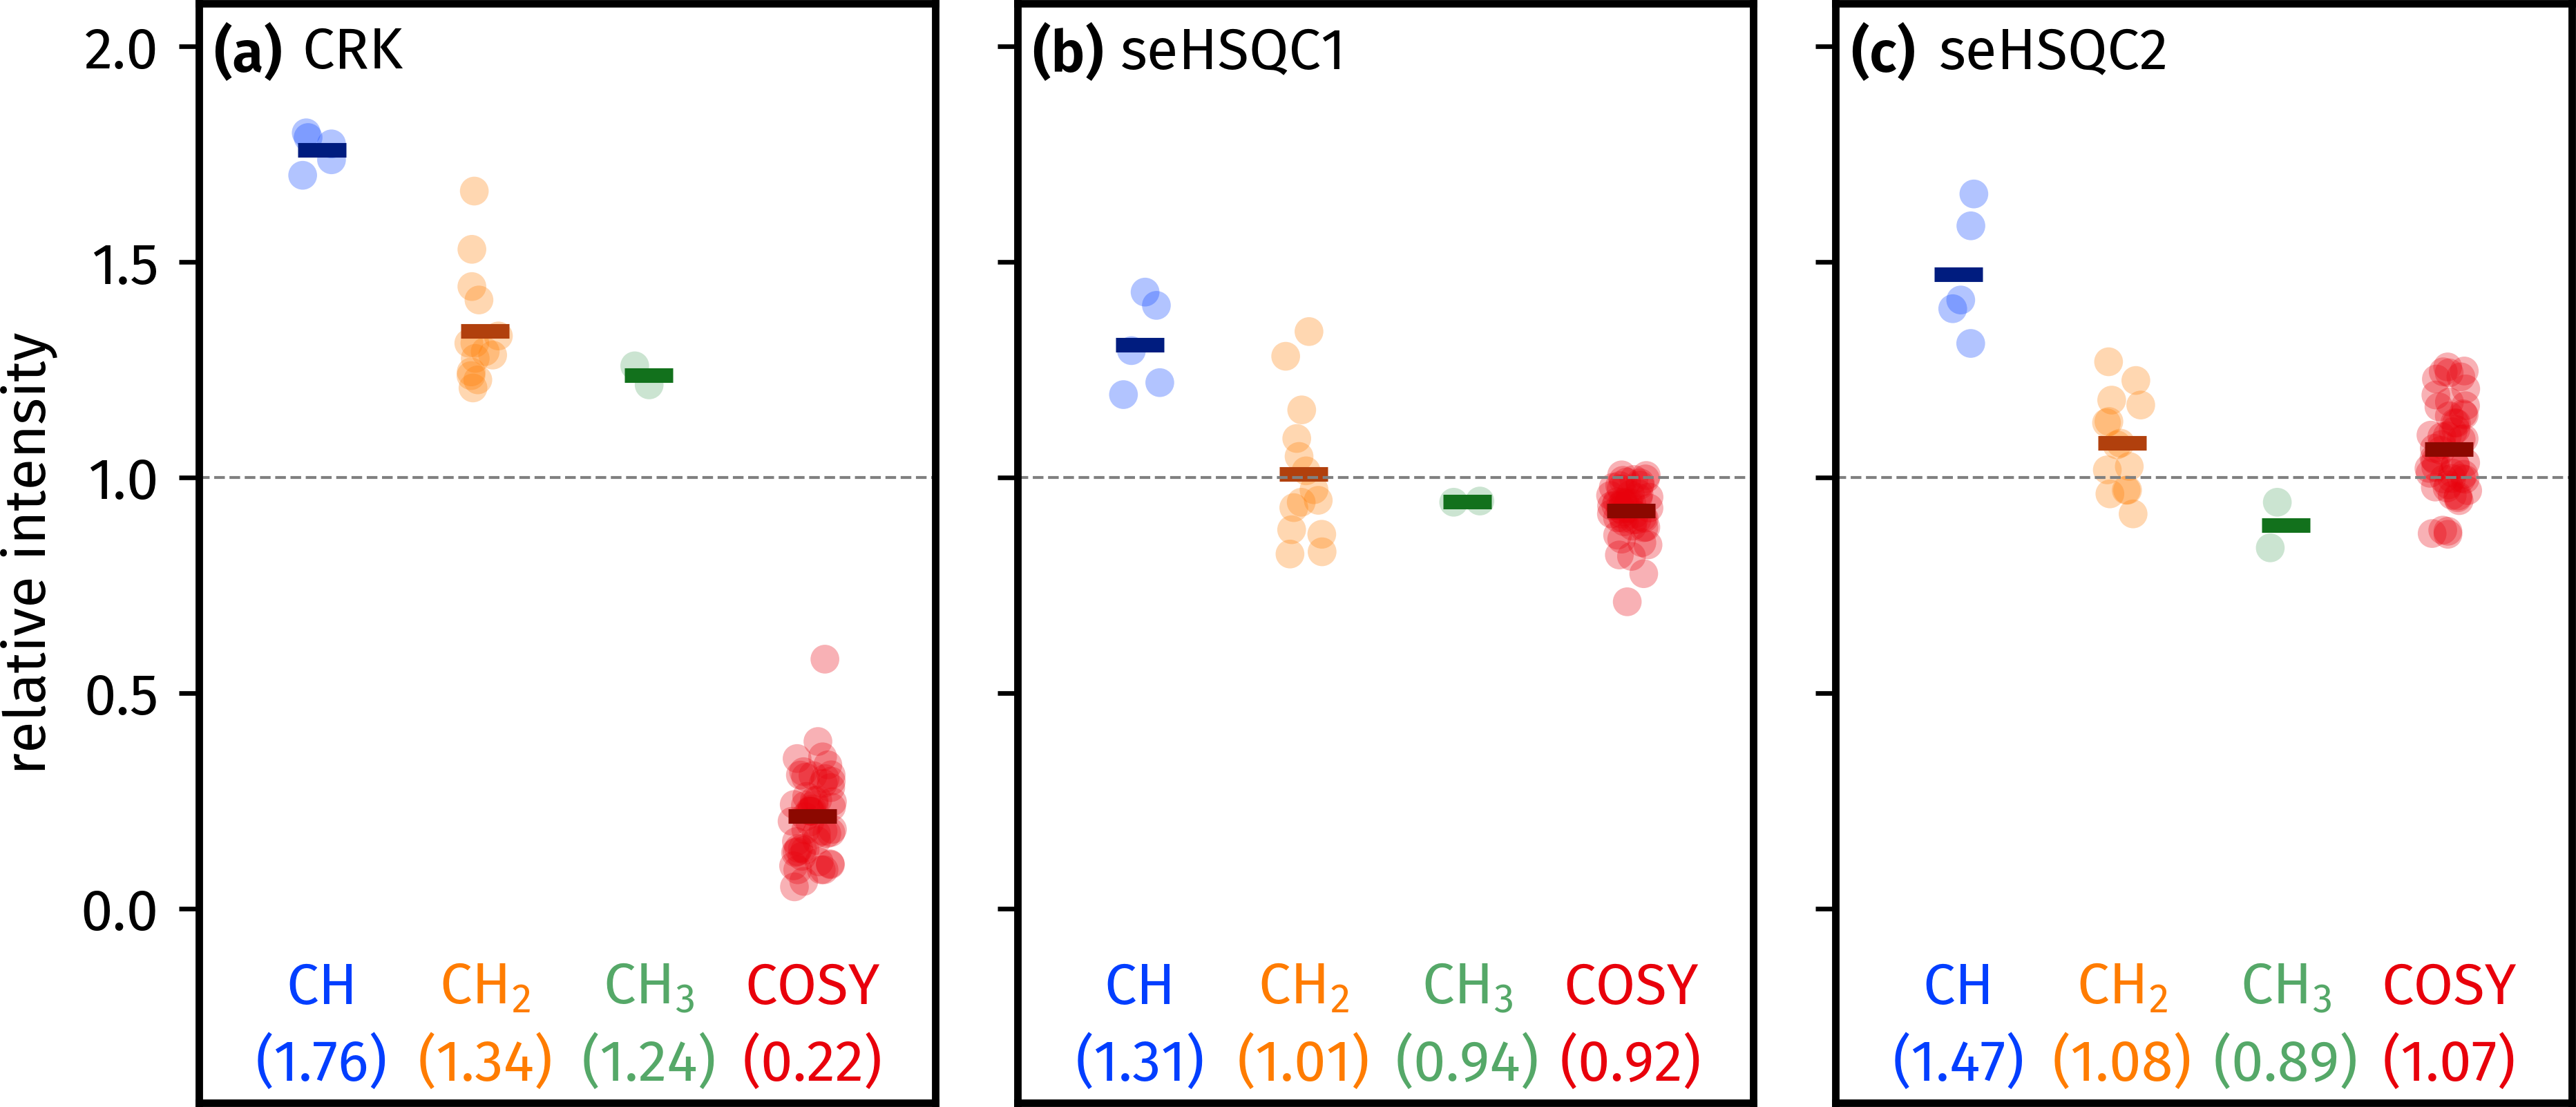
\includegraphics[]{noah/sehsqc_comp_edited.png}%
    {\phantomsubcaption\label{fig:noah_sehsqc_comp_edited_crk}}%
    {\phantomsubcaption\label{fig:noah_sehsqc_comp_edited_1}}%
    {\phantomsubcaption\label{fig:noah_sehsqc_comp_edited_2}}%
    \caption[Sensitivity comparisons for multiplicity-edited seHSQC]{
        Sensitivity comparisons for multiplicity-edited seHSQC in \noah{Sp,Cc} supersequences.
        The delay $\Delta'$ was set to $1 / (8 \cdot \oneJ{CH})$.
        \textbf{(\subref*{fig:noah_sehsqc_comp_edited_crk})} Using the edited CRK seHSQC.
        \textbf{(\subref*{fig:noah_sehsqc_comp_edited_1})} Using the edited seHSQC1 module.
        \textbf{(\subref*{fig:noah_sehsqc_comp_edited_2})} Using the edited seHSQC2 module.
        \datacode{7A-201115}
    }
    \label{fig:noah_sehsqc_comp_edited}
\end{figure}

The inclusion of editing does not make a substantial difference in the sensitivity comparisons (\cref{fig:noah_sehsqc_comp_edited}).
However, it is interesting to note that the edited seHSQC2 in fact performs \textit{better} than the edited HSQC in terms of preserving bulk magnetisation, as evidenced by the larger COSY intensities in \cref{fig:noah_sehsqc_comp_edited_2}.
This can be explained by the fact that in the editing period of the HSQC experiment (and seHSQC1), the bulk magnetisation is placed in the transverse plane.
The evolution of homonuclear couplings will thus lead to a small loss in the amount of \magnnot{C} magnetisation preserved.
In the seHSQC2 sequence, the bulk magnetisation is longitudinal during the editing period, so does not evolve under $J_{\ch{HH}}$.


\subsubsection{Choice of $\symbf{\Delta'}$}

As discussed previously, there are several possible values for the delay $\Delta'$.
I thus also investigated the possibility of setting $\Delta' = 1 / (4 \cdot \oneJ{CH})$.
The corresponding sensitivity comparisons are shown in \cref{fig:noah_sehsqc_1over4j}.

\begin{figure}[!ht]
    \centering
    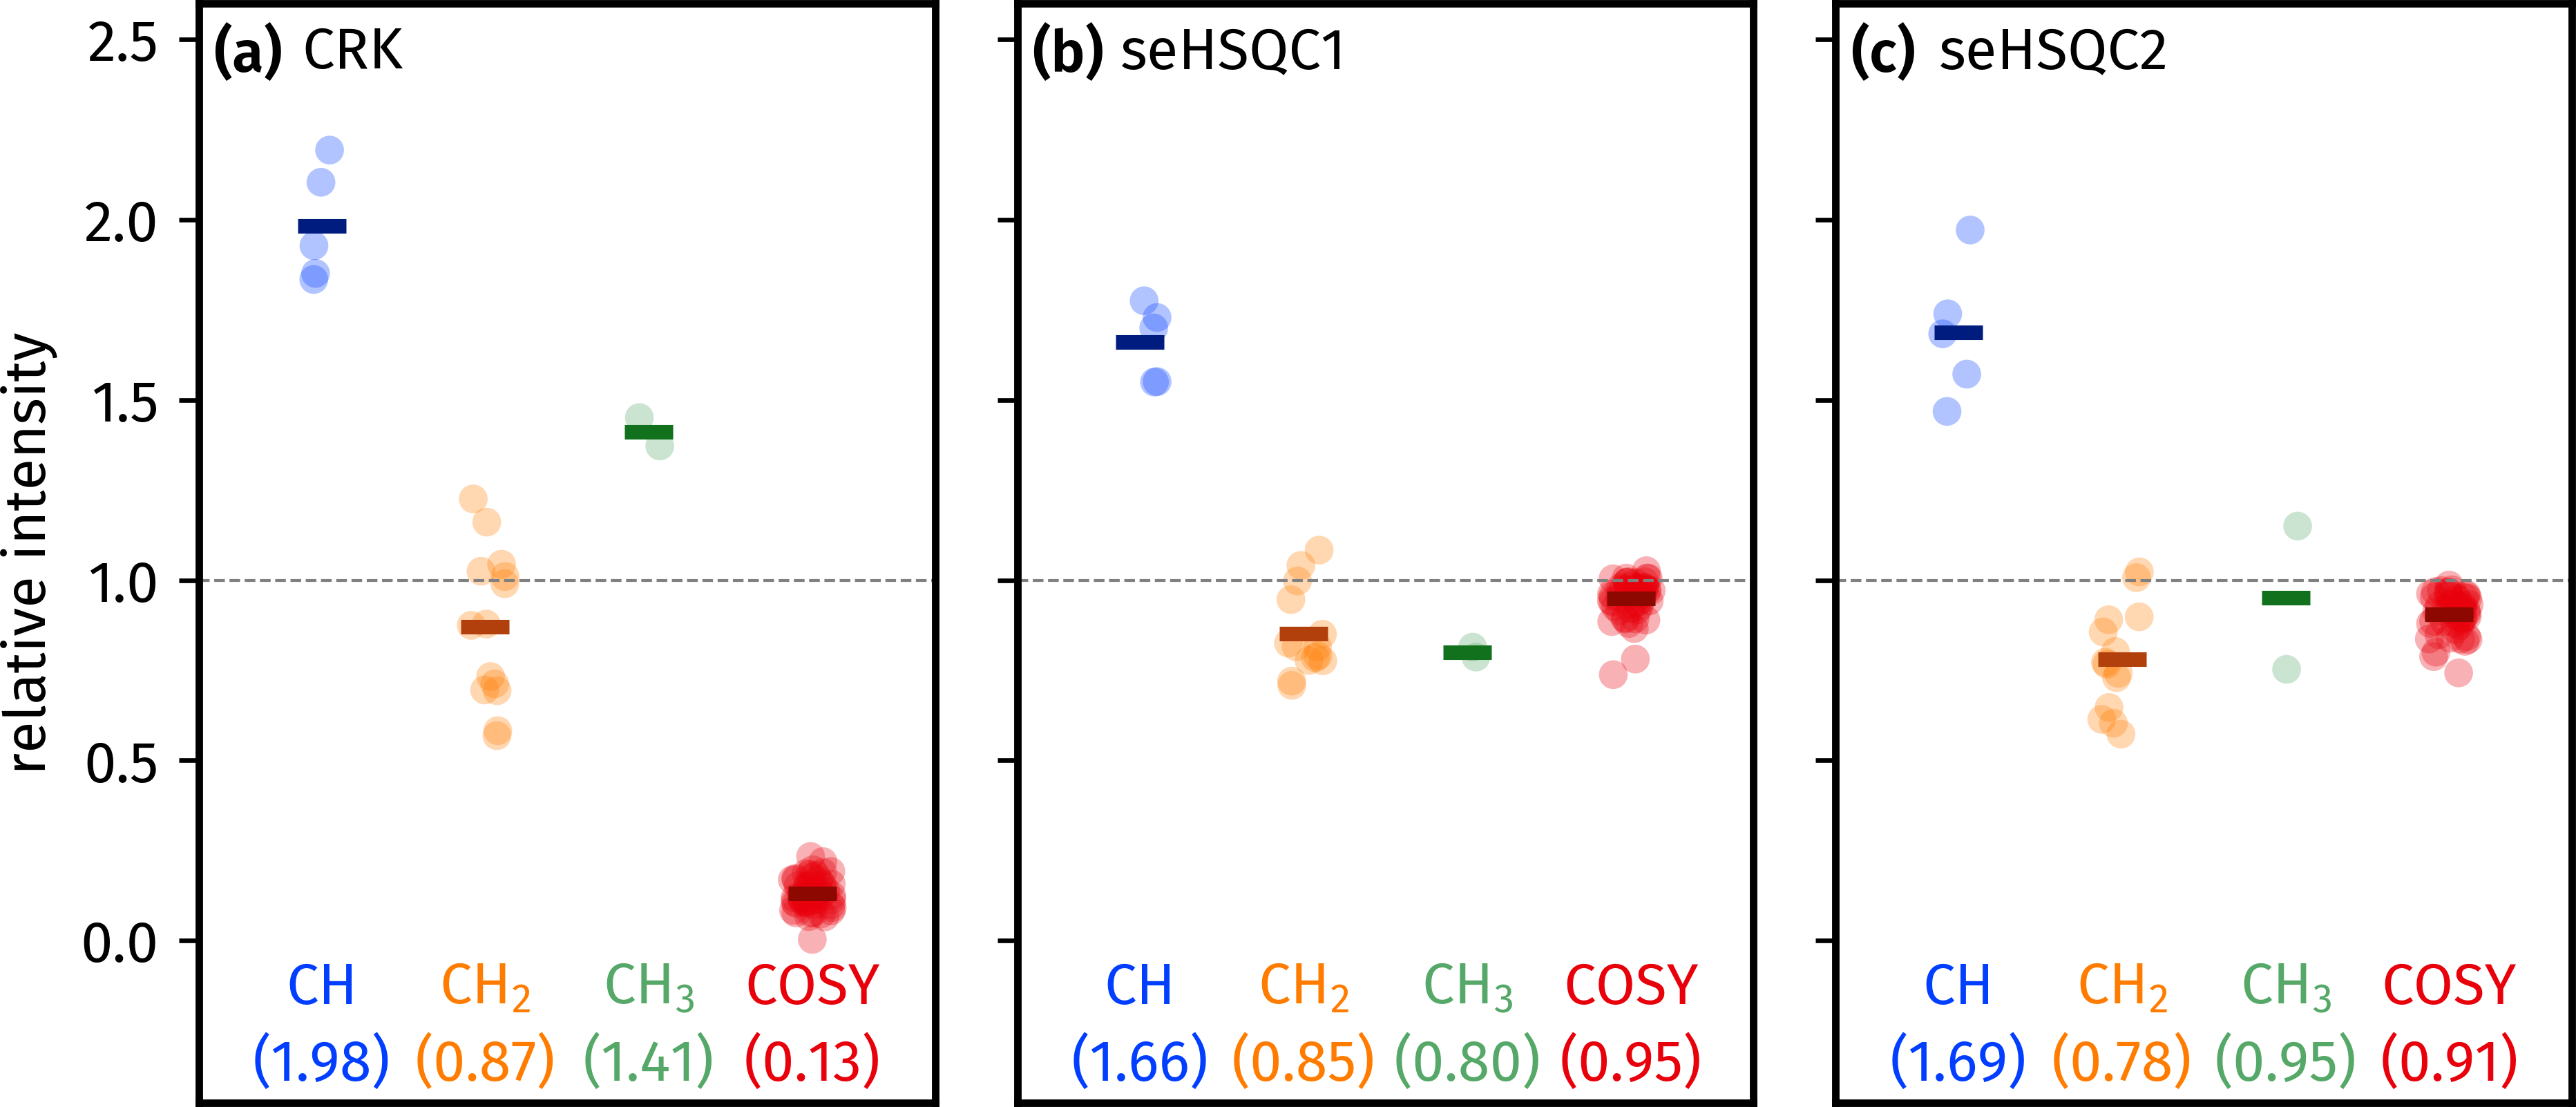
\includegraphics[]{noah/sehsqc_1over4j.png}%
    {\phantomsubcaption\label{fig:noah_sehsqc_1over4j_crk}}%
    {\phantomsubcaption\label{fig:noah_sehsqc_1over4j_1}}%
    {\phantomsubcaption\label{fig:noah_sehsqc_1over4j_2}}%
    \caption[Sensitivity comparisons for seHSQC with $\Delta' = 1 / (4 \cdot \oneJ{CH})$]{
        Sensitivity comparisons with $\Delta'$ set to $1 / (4 \cdot \oneJ{CH})$.
        Multiplicity editing was not used.
        \textbf{(\subref*{fig:noah_sehsqc_1over4j_crk})} Using the CRK seHSQC.
        \textbf{(\subref*{fig:noah_sehsqc_1over4j_1})} Using the seHSQC1 module.
        \textbf{(\subref*{fig:noah_sehsqc_1over4j_2})} Using the seHSQC2 module.
        \datacode{7A-201115}
    }
    \label{fig:noah_sehsqc_1over4j}
\end{figure}

As can be appreciated, the sensitivity boosts obtained for \ch{CH} groups is higher than in the corresponding spectra with $\Delta' = 1 / (8 \cdot \oneJ{CH}$ (\cref{fig:noah_sehsqc_comp}).
However, in this case, there is a small sensitivity \textit{loss} for \ch{CH2} and \ch{CH3} groups as compared to the original HSQC (which is consistent with previous studies\autocite{Schleucher1994JBNMR}).
For \ch{CH3} groups this is unlikely to be of any consequence, but particularly for diastereotopic \ch{CH2} groups this may not be desirable.

It is interesting to note that the performance of the seHSQC1 module is much closer to that of the seHSQC2 here.
The fact that seHSQC1 performs worse with the reduced value of $\Delta' = 1 / (8 \cdot \oneJ{CH})$ suggests that there are some inefficiencies in this section of the pulse sequence; however, there is no immediate explanation for this in the product operators (the relevant terms in the seHSQC1 are entirely similar to that in the CRK, save for a minus sign).

The conclusions drawn are entirely similar when multiplicity editing is enabled (\cref{fig:noah_sehsqc_1over4j_edited}), so will not be further discussed.

\begin{figure}[!ht]
    \centering
    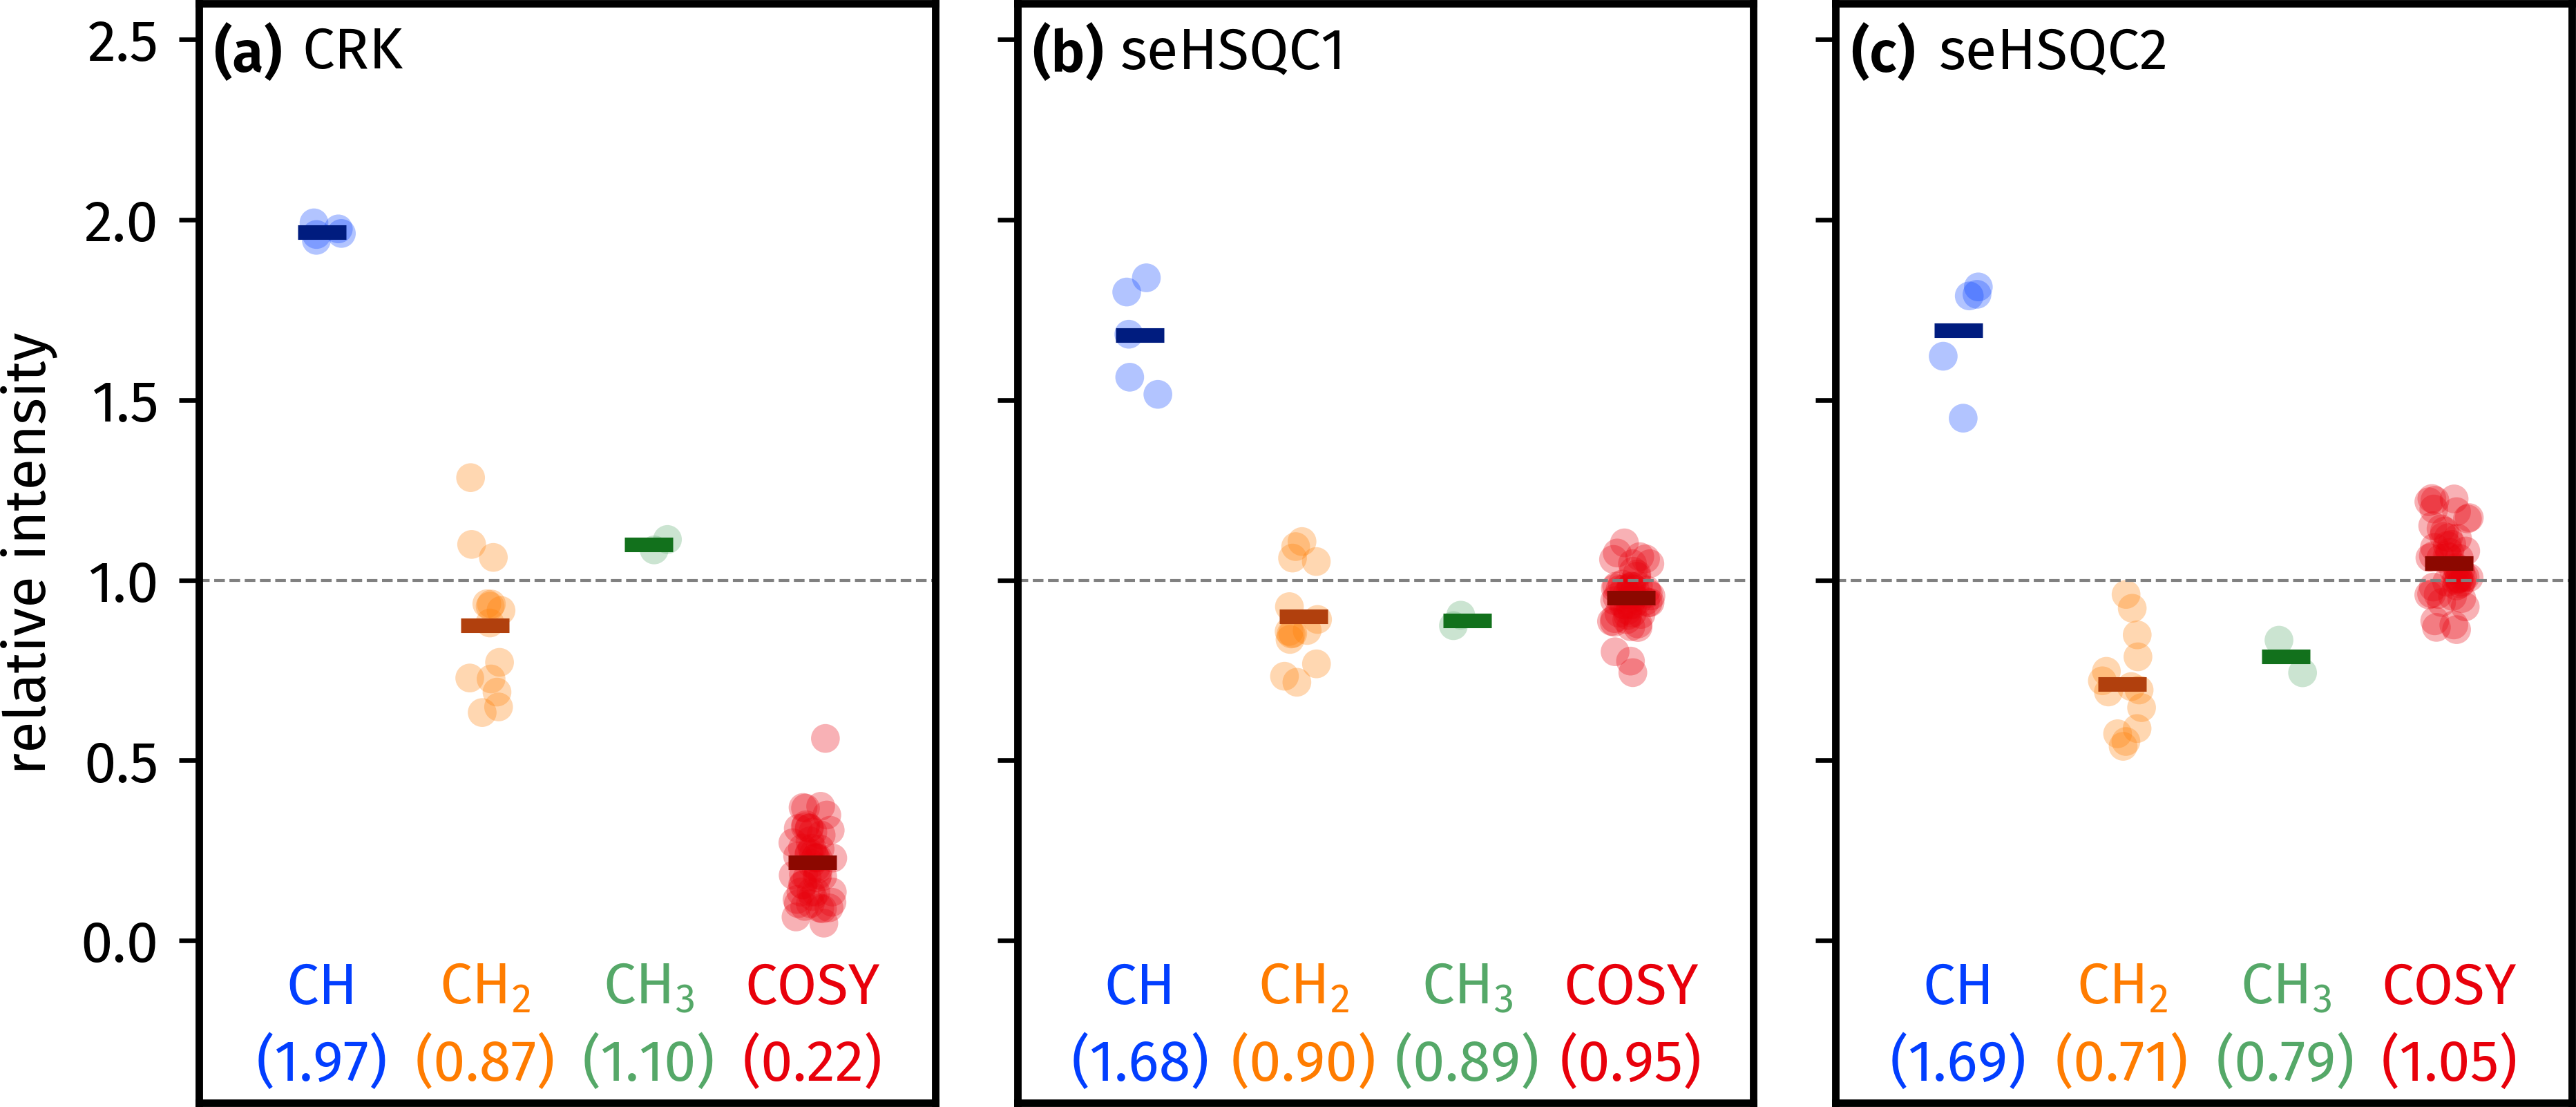
\includegraphics[]{noah/sehsqc_1over4j_edited.png}%
    {\phantomsubcaption\label{fig:noah_sehsqc_1over4j_edited_crk}}%
    {\phantomsubcaption\label{fig:noah_sehsqc_1over4j_edited_1}}%
    {\phantomsubcaption\label{fig:noah_sehsqc_1over4j_edited_2}}%
    \caption[Sensitivity comparisons for edited seHSQC with $\Delta' = 1 / (4 \cdot \oneJ{CH})$]{
        Sensitivity comparisons with $\Delta'$ set to $1 / (4 \cdot \oneJ{CH})$ and with multiplicity editing.
        \textbf{(\subref*{fig:noah_sehsqc_1over4j_edited_crk})} Using the edited CRK seHSQC.
        \textbf{(\subref*{fig:noah_sehsqc_1over4j_edited_1})} Using the edited seHSQC1 module.
        \textbf{(\subref*{fig:noah_sehsqc_1over4j_edited_2})} Using the edited seHSQC2 module.
        \datacode{7A-201115}
    }
    \label{fig:noah_sehsqc_1over4j_edited}
\end{figure}




\subsubsection{Optimal control for seHSQC1}

One unresolved question is why the seHSQC1 module has a lower sensitivity than the seHSQC2, despite being shorter and containing fewer \ang{180} pulses.
There is also nothing in the product operator analysis to explain why this should be the case.
One remaining possibility is the presence of some non-ideality in the pulses themselves, and the composite \proton{} pulse is an obvious candidate for investigation.%
\footnote{The concept of a \textit{composite pulse}\autocite{Levitt1986PNMRS} is usually associated with greater efficiency / uniformity, but here I have used the term to loosely refer to a consecutive series of pulses.}

In order to investigate the extent to which this was responsible, I sought to use optimal control theory to develop a \textit{universal rotation pulse} (URP) which could replace this composite pulse.
Such a pulse must accomplish the transformations in \cref{eq:sehsqc1_dp}, namely $z \to y$ and $y \to x$.%
\footnote{The effect of this pulse on $x$-magnetisation is not important for the seHSQC1, but is in fact fully determined by these two constraints: $UI_x\adj{U} = -\mi U(I_yI_z - I_zI_y)\adj{U} = -\mi(UI_y\adj{U}UI_z\adj{U} - UI_z\adj{U}UI_y\adj{U}) = -\mi(I_xI_y - I_yI_x) = I_z$.
This reveals a geometric interpretation of this pulse element: it is actually a \ang{120} rotation about the vector $(1, 1, 1)$, which is closely related to the $C_3$ symmetry operation in the octahedral point group.}
This optimisation was performed using an interior-point algorithm (the default in Matlab \texttt{fmincon}) and the ESCALADE method\autocite{Foroozandeh2021A} for the calculation of analytic derivatives.
Pulse fidelity was calculated as an average over 51 \proton{} spins, evenly distributed across a frequency range of \qty{11}{kHz} (corresponding to \qty{15.7}{\ppm} at \qty{700}{\MHz}); the duration of the pulse was fixed at \qty{200}{\us}, and 200 pulse points were used.

The \carbon{} \ang{90} pulse which is simultaneously applied during the pulse sequence was not optimised together with this: because of the longer duration of the \proton{} URP, the sequence must be modified slightly (\cref{fig:sehsqc1_urp}).
In particular, the delays $\alpha$ and $\beta$ must be chosen in order to satisfy the relations $2\varepsilon = \alpha + \beta$ (to ensure \magnnot{C} magnetisation is refocused), and $\alpha = \beta + \tau$ (to ensure that for \magn{C} magnetisation, the \carbon{} chemical shift evolves for a total duration of $t_1$).

\begin{figure}[!ht]
    \centering
    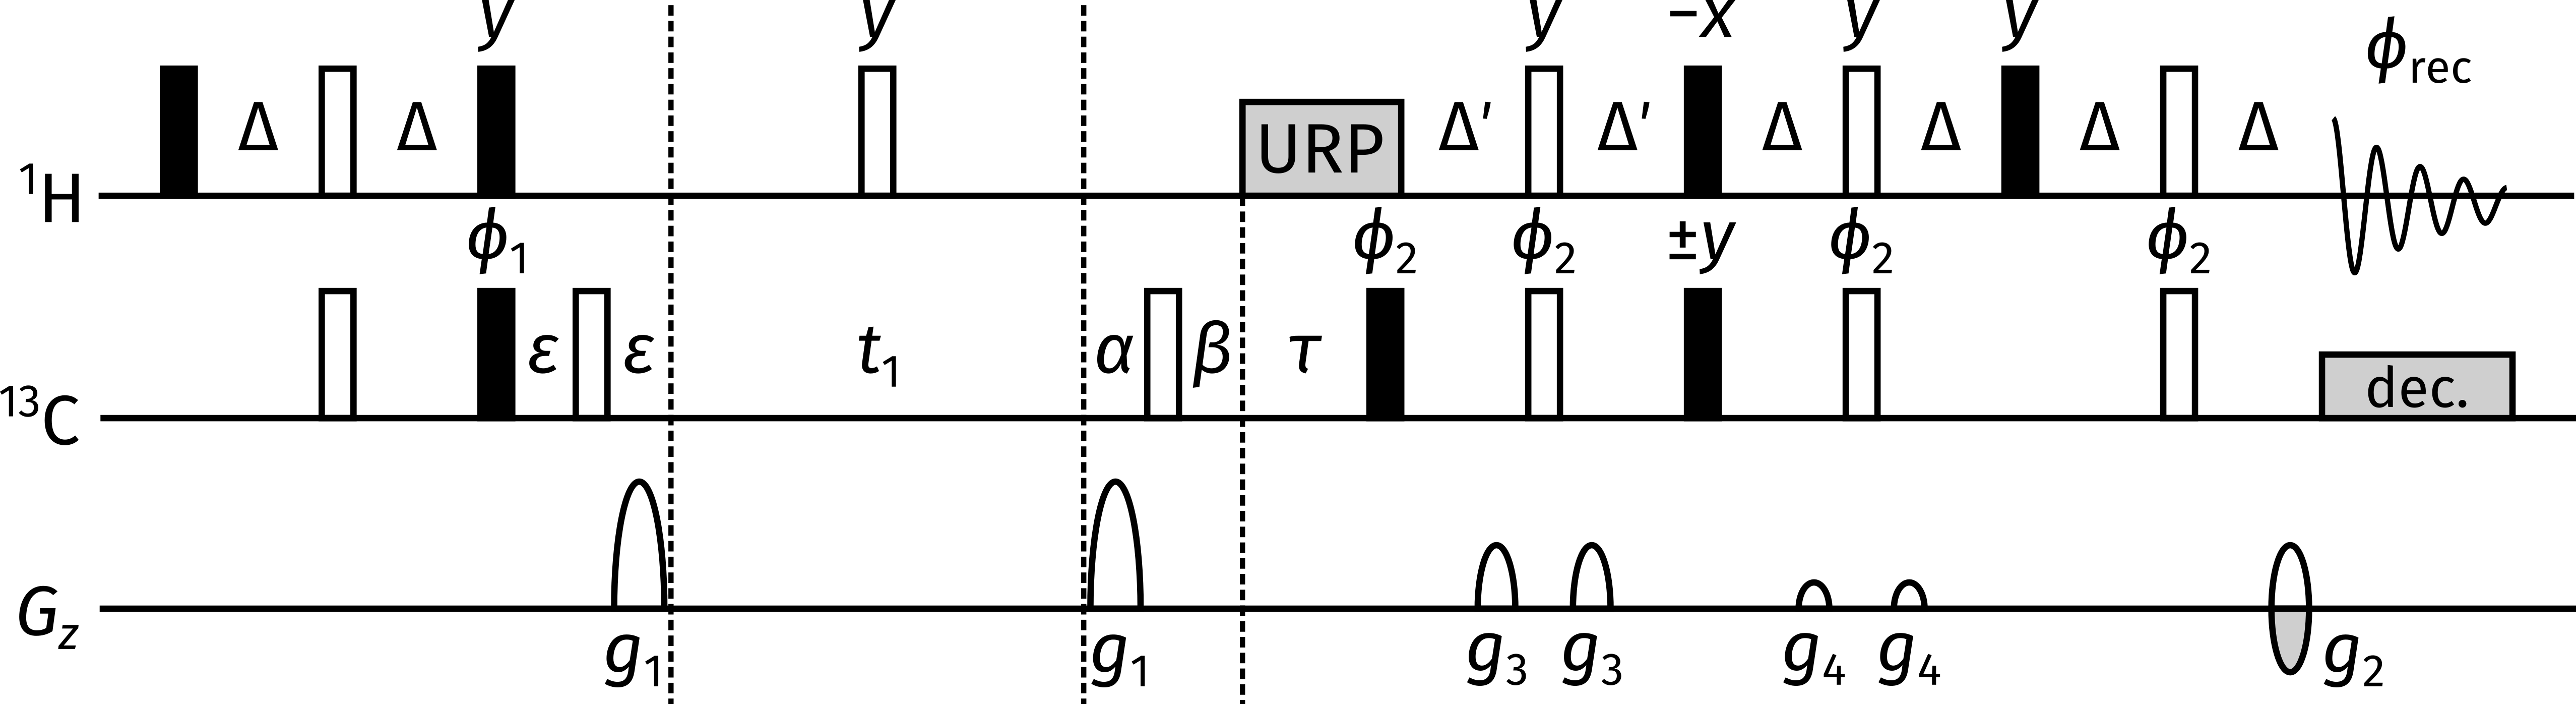
\includegraphics[]{pp/sehsqc/1urp.png}%
    \caption[seHSQC1 pulse sequence with \proton{} URP]{
        seHSQC1 pulse sequence using a \proton{} URP in place of the double-\ang{90} composite pulse.
        $\tau$ is the difference in duration between the URP and the \carbon{} \ang{90} hard pulse.
        Delays are set as: $\alpha = \varepsilon + \tau/2$; $\beta = \varepsilon - \tau/2$.
    }
    \label{fig:sehsqc1_urp}
\end{figure}

\begin{figure}[!ht]
    \centering
    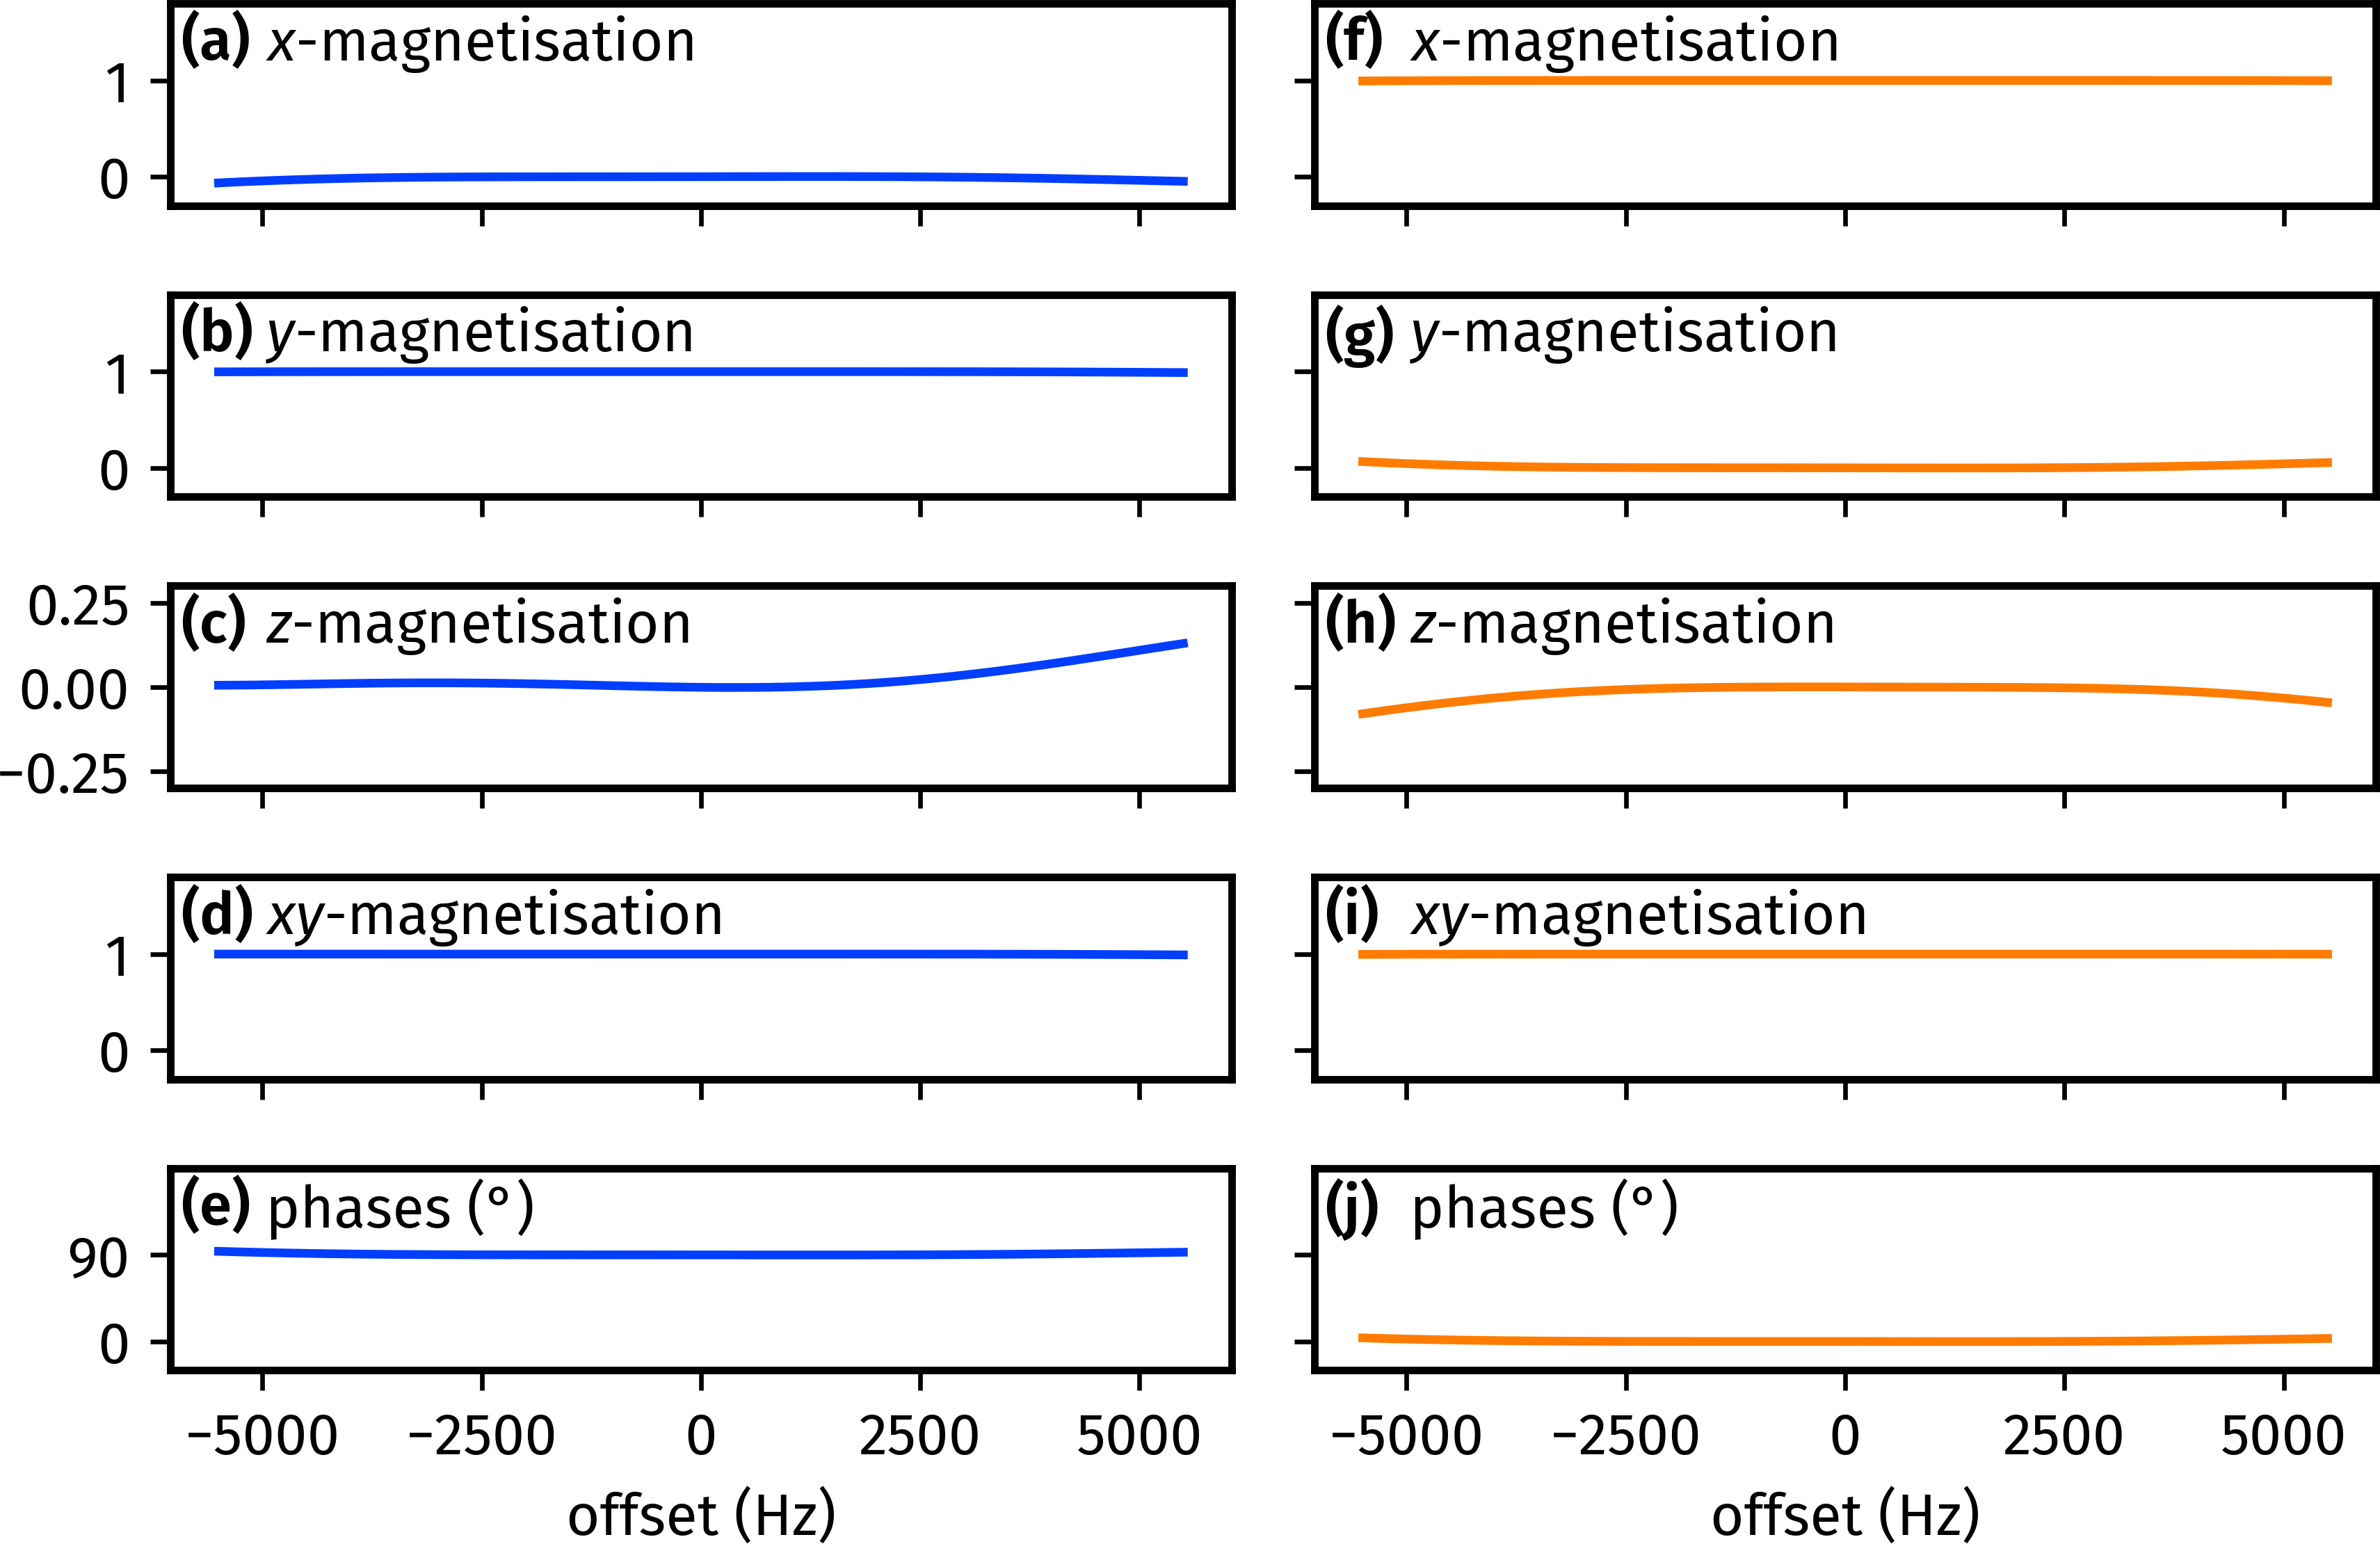
\includegraphics[]{noah/spv1_urp_magn.png}%
    {\phantomsubcaption\label{fig:spv1_urp_magn_z_x}}%
    {\phantomsubcaption\label{fig:spv1_urp_magn_z_y}}%
    {\phantomsubcaption\label{fig:spv1_urp_magn_z_z}}%
    {\phantomsubcaption\label{fig:spv1_urp_magn_z_xy}}%
    {\phantomsubcaption\label{fig:spv1_urp_magn_z_phase}}%
    {\phantomsubcaption\label{fig:spv1_urp_magn_y_x}}%
    {\phantomsubcaption\label{fig:spv1_urp_magn_y_y}}%
    {\phantomsubcaption\label{fig:spv1_urp_magn_y_z}}%
    {\phantomsubcaption\label{fig:spv1_urp_magn_y_xy}}%
    {\phantomsubcaption\label{fig:spv1_urp_magn_y_phase}}%
    \caption[Simulated performance of URP used for seHSQC1 module]{
        Simulated performance of URP used for seHSQC1 module on $z$- and $y$-magnetisation. The pulse fidelity was 99.99\%.
        \textbf{(\subref*{fig:spv1_urp_magn_z_x})--(\subref*{fig:spv1_urp_magn_z_phase})} Using $z$-magnetisation as input: the plots respectively show the amount of $x$-magnetisation, $y$-magnetisation, $z$-magnetisation, transverse magnetisation ($M_{xy} = \sqrt{M_x^2 + M_y^2}$), and the phase of the transverse magnetisation generated, as a function of offset frequency.
        \textbf{(\subref*{fig:spv1_urp_magn_y_x})--(\subref*{fig:spv1_urp_magn_y_phase})} The same, but using $y$-magnetisation as input.
    }
    \label{fig:spv1_urp_magn}
\end{figure}

This optimisation process yielded a pulse with 99.99\% fidelity: the (theoretical) performance of this pulse on $z$- and $y$-magnetisation is shown in \cref{fig:spv1_urp_magn}.
However, when tested in the actual seHSQC1 experiment, this failed to yield any substantial difference compared to the original double \ang{90} pulse (\cref{fig:sehsqc1_urp_sens_1dp,fig:sehsqc1_urp_sens_1urp}).
Importantly, the performance still falls below that of the seHSQC2 module (\cref{fig:sehsqc1_urp_sens_2}).
The reason for the poorer sensitivity therefore likely lies elsewhere.

\begin{figure}[htb]
    \centering
    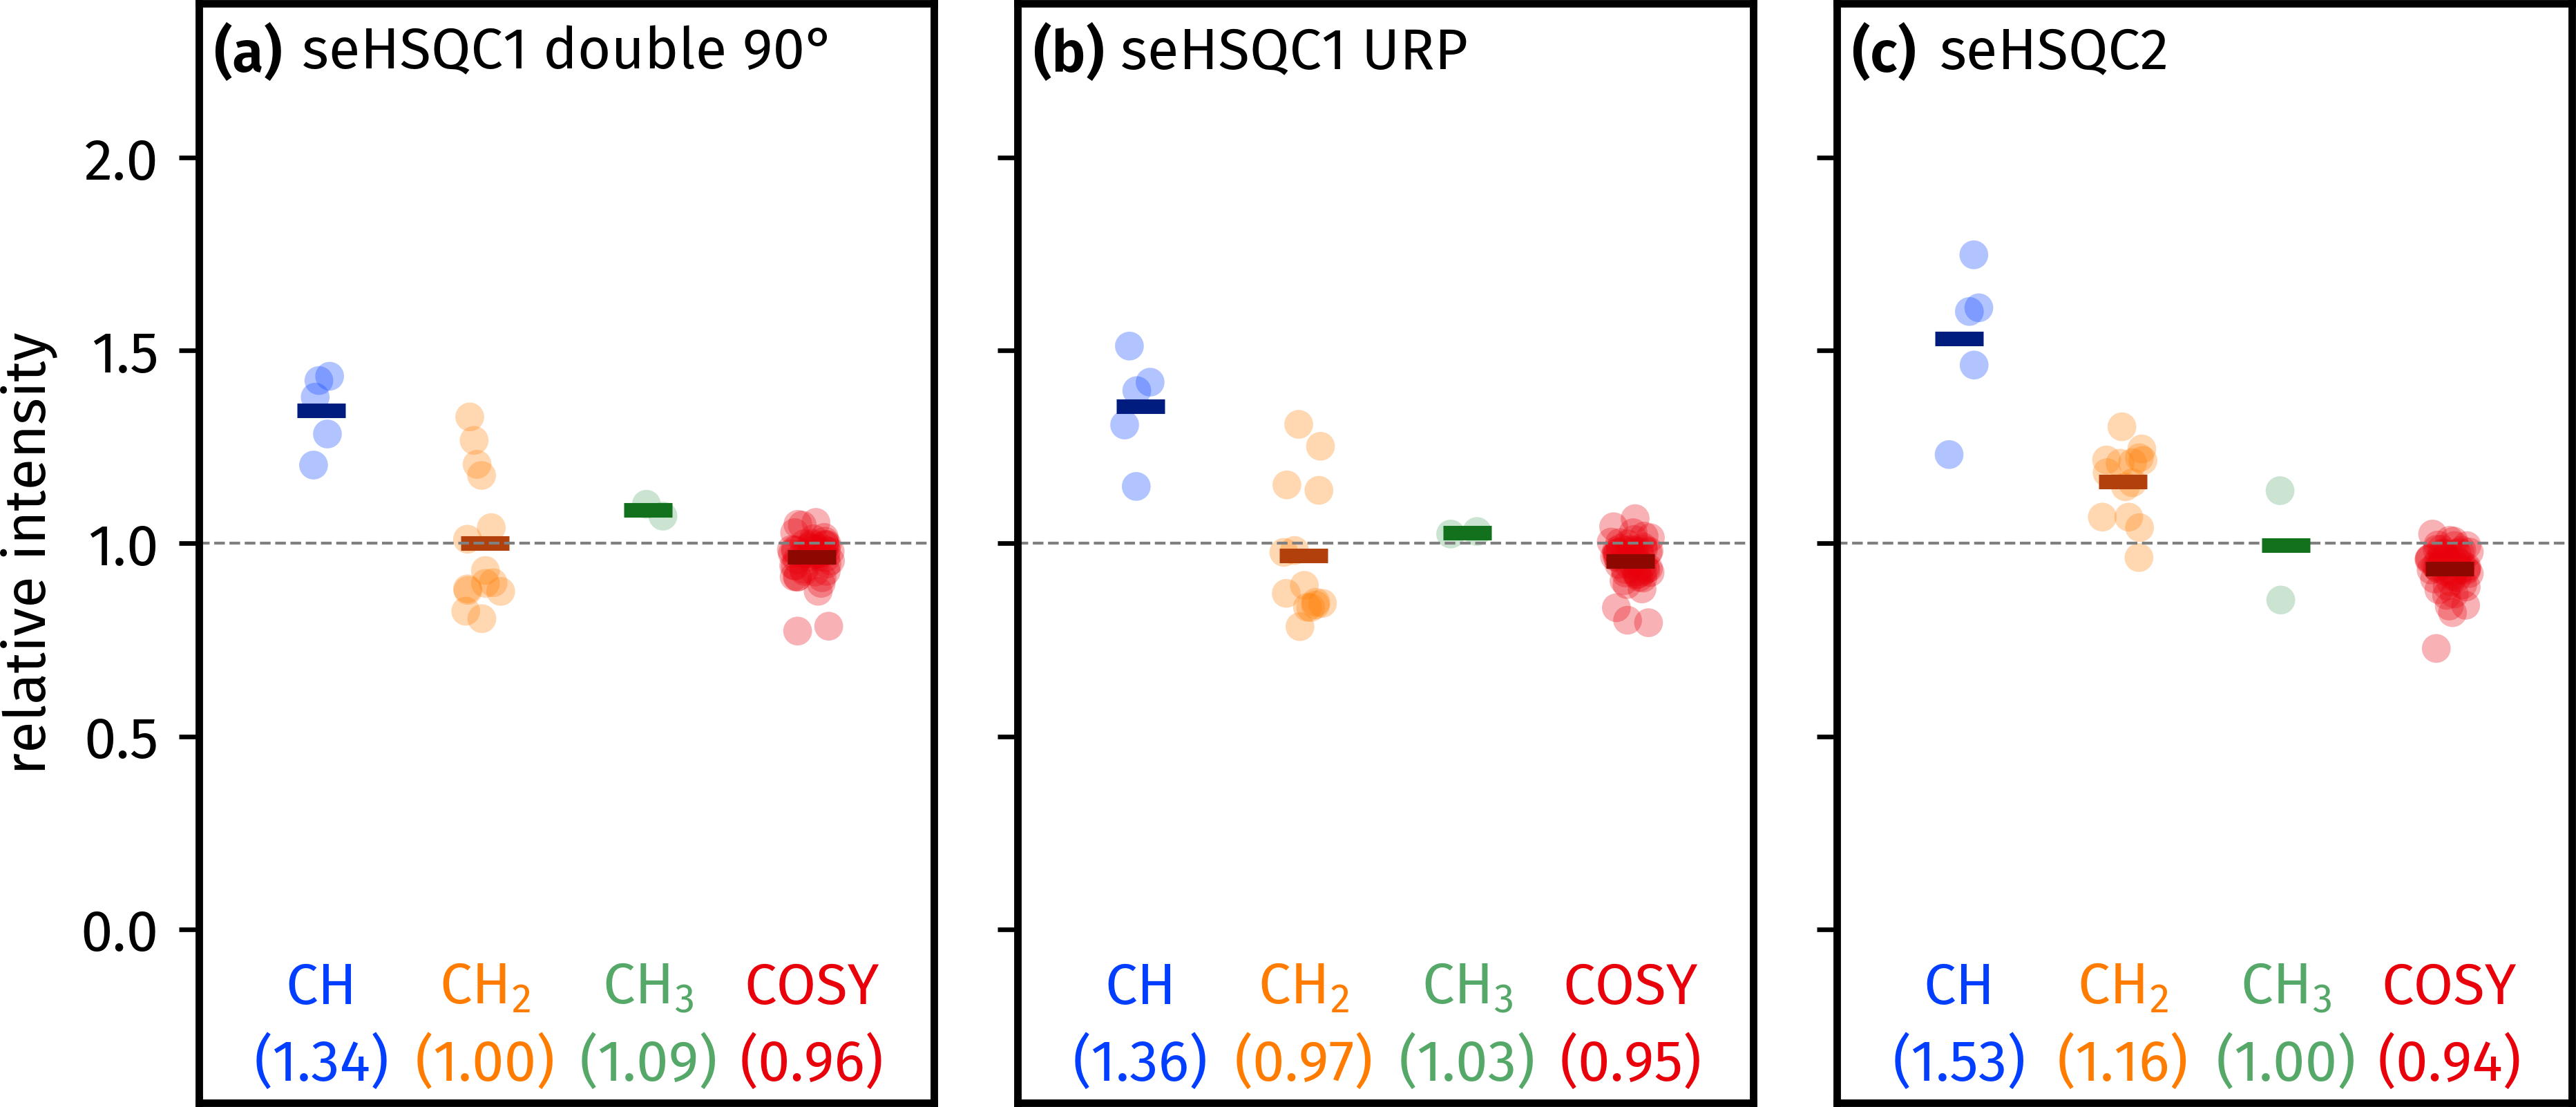
\includegraphics[]{noah/sehsqc1_urp_sens.png}%
    {\phantomsubcaption\label{fig:sehsqc1_urp_sens_1dp}}%
    {\phantomsubcaption\label{fig:sehsqc1_urp_sens_1urp}}%
    {\phantomsubcaption\label{fig:sehsqc1_urp_sens_2}}%
    \caption[Sensitivity comparison of seHSQC1 module with URP]{
        Sensitivity comparisons using the seHSQC1 URP.
        $\Delta'$ was set to $1 / (8 \cdot \oneJ{CH})$; no multiplicity editing was used.
        Note that a different dataset was used for this figure and \cref{fig:noah_sehsqc_comp}, so the numbers are very slightly different.
        \textbf{(\subref*{fig:sehsqc1_urp_sens_1dp})} Original seHSQC1 module with double \proton{} \ang{90} pulse.
        \textbf{(\subref*{fig:sehsqc1_urp_sens_1urp})} seHSQC1 using the optimised URP shown in \cref{fig:spv1_urp_magn}.
        \textbf{(\subref*{fig:sehsqc1_urp_sens_2})} seHSQC2 module for comparison.
        \datacode{7A-220110}
    }
    \label{fig:sehsqc1_urp_sens}
\end{figure}


\subsubsection{BIG-BIRD versus ZIP}

The final point in this section pertains to the implementation of the seHSQC2 module.
As it stands, the isotope-specific rotation element placed at the start of the module is the ZIP element: its role is to effect \ang{90} rotations with different phases on the \magn{C} and \magnnot{C} magnetisation pools.
However, such pulse elements have been known for a long time: these include TANGO\autocite{Wimperis1984JMR}, BANGO\autocite{Sorensen1994BMR}, BIRD\autocite{Garbow1982CPL,Uhrin1993JMRSA,Kaltschnee2014CC}, BIG-BIRD\autocite{Briand1997JMR}, and TIG-BIRD\autocite{Briand1998JMR}.
In particular, the BIG-BIRD element can be designed to accomplish the same overall effect as the ZIP element.
For the seHSQC2 without multiplicity editing, we can therefore replace the ZIP element with
\begin{equation}
    \label{eq:big_bird_unedited}
    45\rlap{\unit{\degree}}_{\ang{45}}(\proton{})\text{--}2\Delta\text{--}\ang{180}(\proton{},\carbon{})\text{--}2\Delta\text{--}45\rlap{\unit{\degree}}_{\ang{225}}(\proton{}),
\end{equation}
where $\beta_\phi$ represents a hard pulse with flip angle $\beta$ and phase $\phi$.
For the edited seHSQC, the phases must be altered slightly:
\begin{equation}
    \label{eq:big_bird_edited}
    45\rlap{\unit{\degree}}_{\ang{315}}(\proton{})\text{--}2\Delta\text{--}\ang{180}(\proton{},\carbon{})\text{--}2\Delta\text{--}45\rlap{\unit{\degree}}_{\ang{135}}(\proton{}).
\end{equation}
This BIG-BIRD version of the seHSQC2 was also evaluated.
However, its performance in all respects was not as good as the ZIP version: both the seHSQC sensitivity itself, as well as the sensitivity of the later CLIP-COSY, were lower when the BIG-BIRD element was used.

\begin{figure}[!ht]
    \centering
    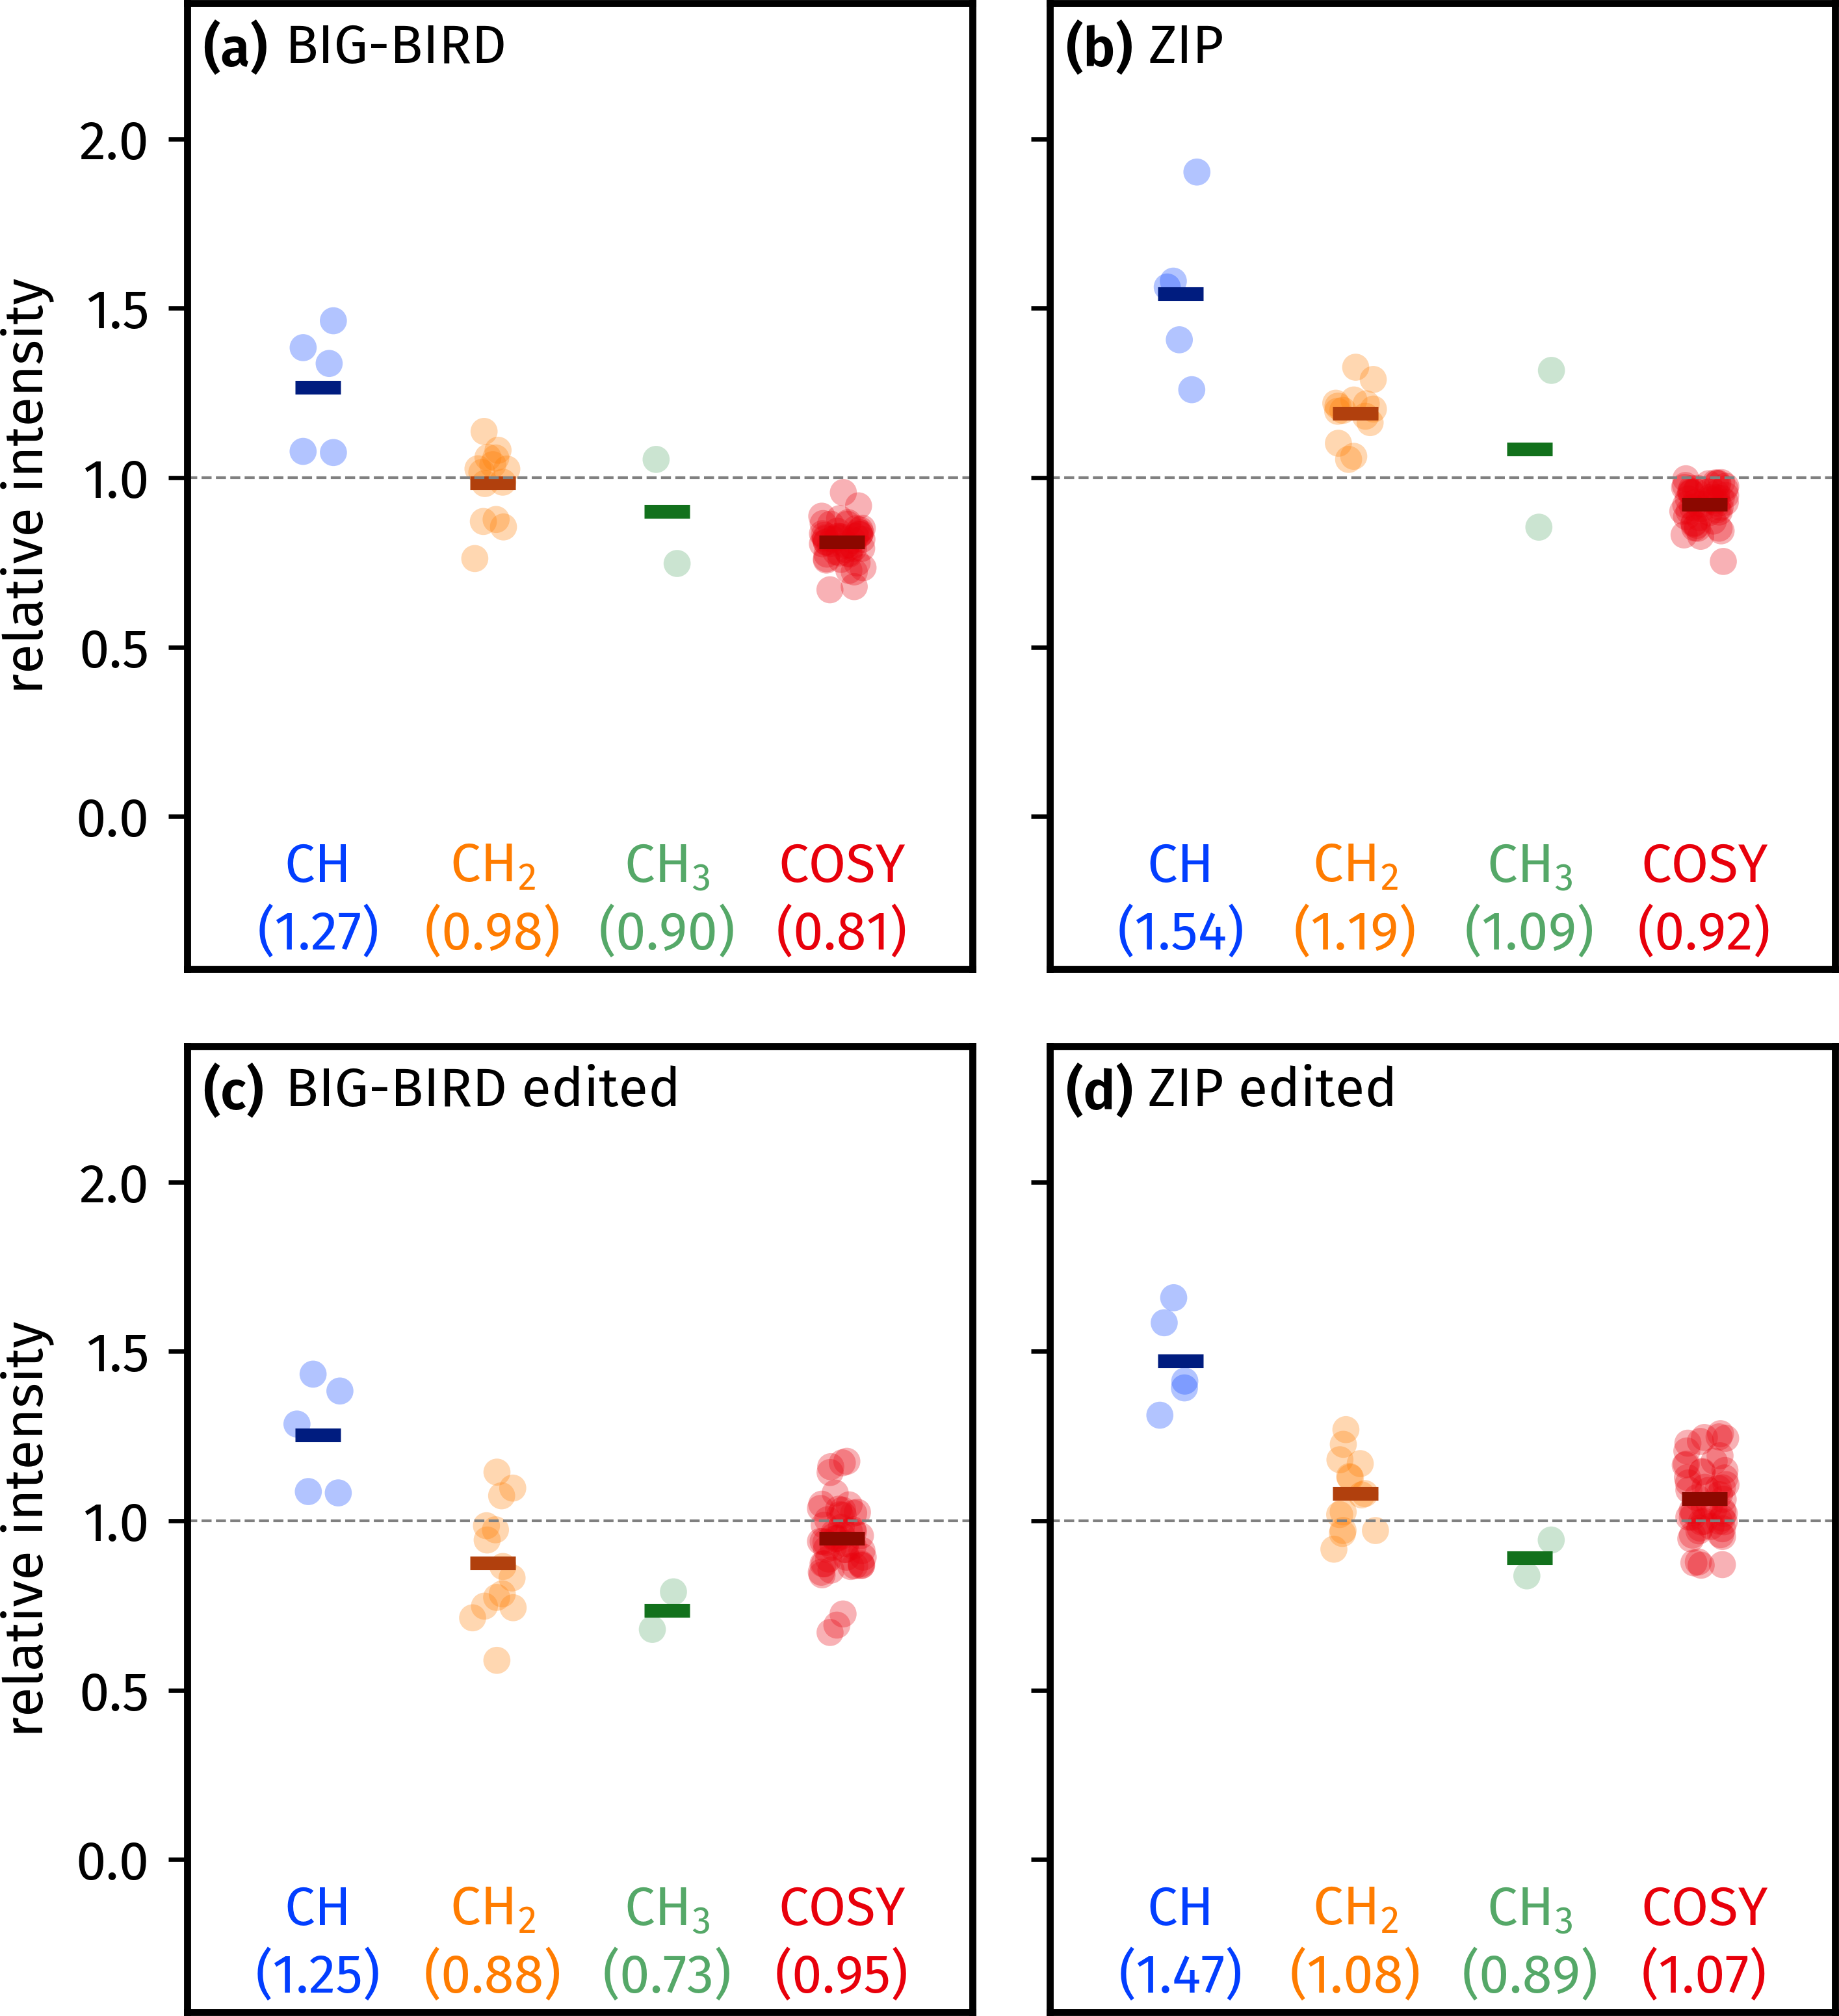
\includegraphics[]{noah/sehsqc_bigbird.png}%
    {\phantomsubcaption\label{fig:noah_sehsqc_bigbird_bb_noed}}%
    {\phantomsubcaption\label{fig:noah_sehsqc_bigbird_zip_noed}}%
    {\phantomsubcaption\label{fig:noah_sehsqc_bigbird_bb_ed}}%
    {\phantomsubcaption\label{fig:noah_sehsqc_bigbird_zip_ed}}%
    \caption[Comparison of BIG-BIRD and ZIP pulse elements in seHSQC2 module]{
        Sensitivity comparisons of BIG-BIRD and ZIP pulse elements in seHSQC2 module.
        The reference dataset being compared against is still the \noah{S,Cc} (but with editing in (\subref*{fig:noah_sehsqc_bigbird_bb_ed}) and (\subref*{fig:noah_sehsqc_bigbird_zip_ed}).
        The delay $\Delta'$ was set to $1 / (8 \cdot \oneJ{CH})$.
        \textbf{(\subref*{fig:noah_sehsqc_bigbird_bb_noed})} Unedited seHSQC2 using BIG-BIRD.
        \textbf{(\subref*{fig:noah_sehsqc_bigbird_zip_noed})} Unedited seHSQC2 using ZIP.
        \textbf{(\subref*{fig:noah_sehsqc_bigbird_bb_ed})} Edited seHSQC2 using BIG-BIRD.
        \textbf{(\subref*{fig:noah_sehsqc_bigbird_zip_ed})} Edited seHSQC2 using ZIP.
        \datacode{7A-201115}
    }
    \label{fig:noah_sehsqc_bigbird}
\end{figure}

\subsection{\texorpdfstring{\nitrogen{}}{15N} sensitivity-enhanced HSQC}
\label{subsec:noah__sehsqc_n}

\nitrogen{} seHSQC


\subsection{\texorpdfstring{\nitrogen{}}{15N} HMQC}
\label{subsec:noah__hmqc}

In \cref{subsec:noah__sehsqc_n}, I will discuss how the sensitivity-enhanced HSQC modules developed above may be adapted into \proton{}--\nitrogen{} experiments.
However, before that, I make a slight detour to cover the \nitrogen{} HMQC experiment, which (up until my DPhil) was the experiment of choice for detecting one-bond \proton{}--\nitrogen{} correlations.

\begin{figure}[htb]
    \centering
    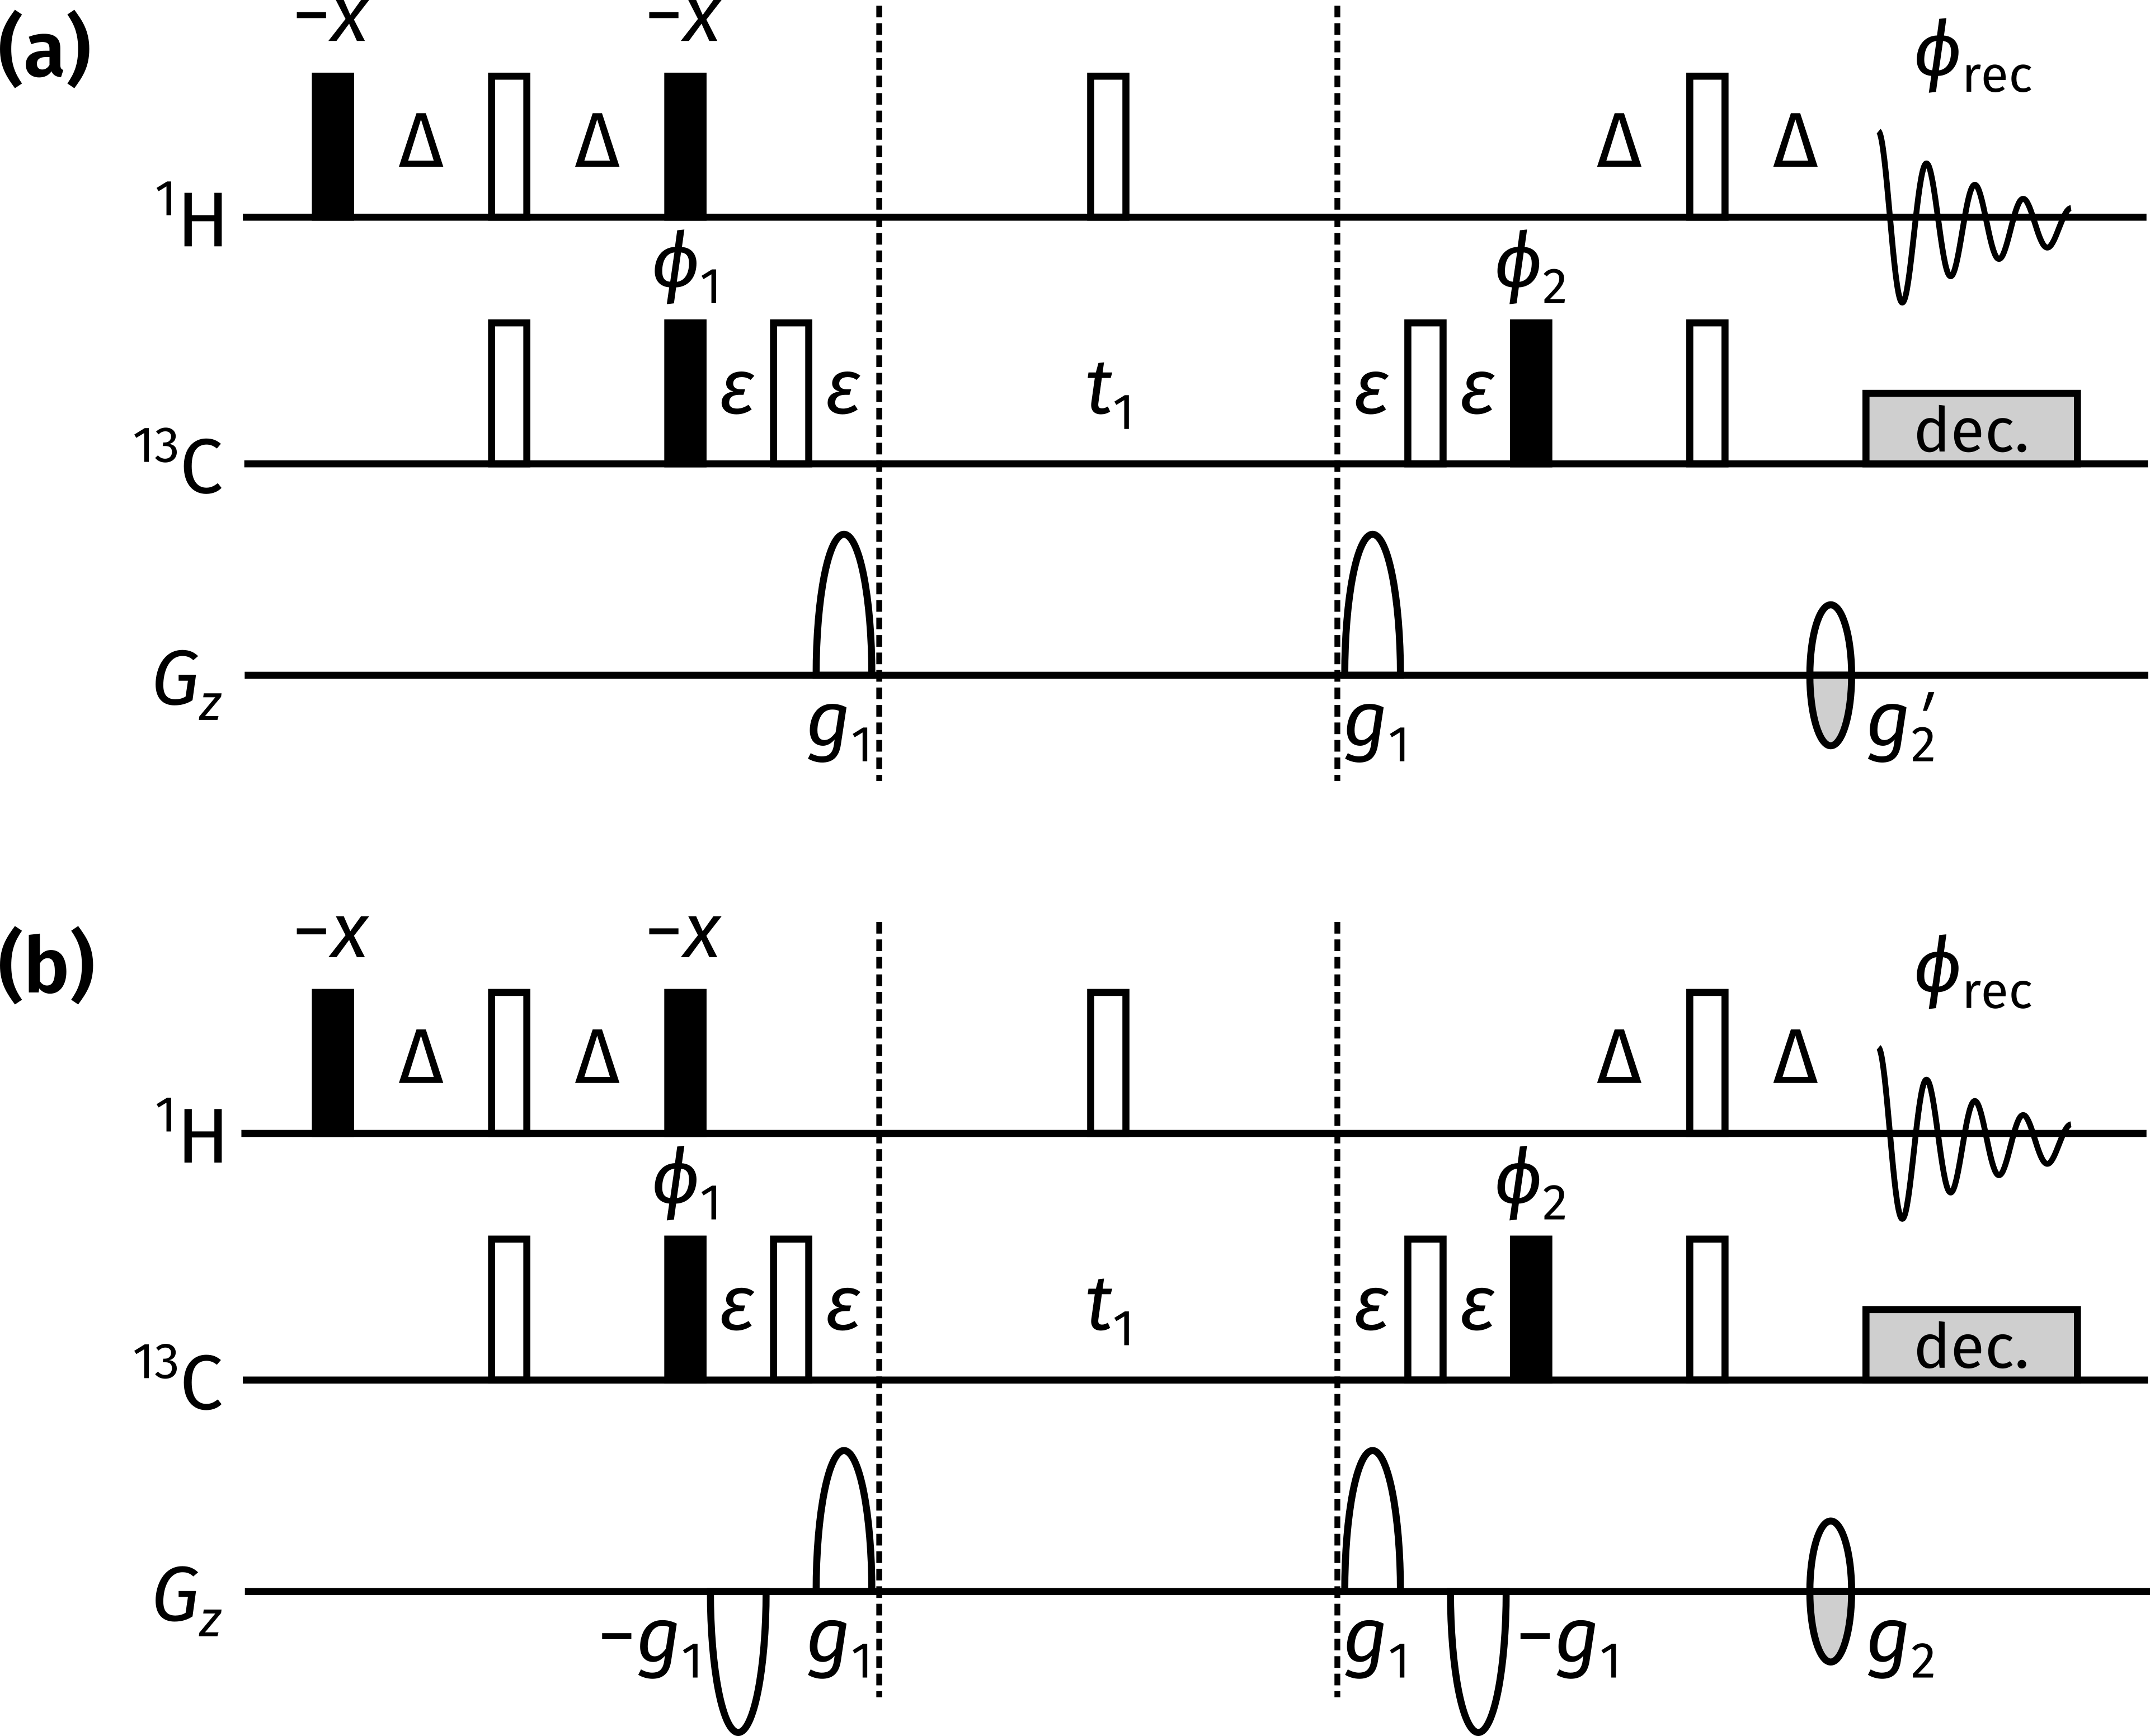
\includegraphics[draft=false]{pp/hmqc/all.png}%
    {\phantomsubcaption\label{fig:noah_hmqc_2grad}}%
    {\phantomsubcaption\label{fig:noah_hmqc_4grad}}%
    \caption[NOAH HMQC pulse sequences]{
        \textbf{(\subref*{fig:noah_hmqc_2grad})} With two encoding gradients around $t_1$.
        \textbf{(\subref*{fig:noah_hmqc_4grad})} With four encoding gradients around $t_1$.
        Phase cycling is performed with $\phi_1 = (x, -x)$, $\phi_2 = (x, x, -x, -x)$, and $\phi_\text{rec} = (x, -x, -x, x)$.
        The delay $\Delta$ is set to $1 / (4 \cdot \oneJ{NH})$.
        Gradient amplitudes are: $g_1 = 80\%$; $g_2 = \pm 32.4\%$; $g_2' = g_2/2$.
    }
    \label{fig:noah_hmqc}
\end{figure}


\subsubsection{CTP gradient scheme}

The HMQC module is based on the ASAP-HMQC reported by Kup{\v{c}}e and Freeman\autocite{Kupce2007MRC}, which used a symmetric gradient scheme similar to that in the seHSQC modules previously described (\cref{fig:noah_hmqc_2grad}).
However, in the NOAH module\autocite{Kupce2017ACIE}, bipolar gradient pulse pairs were placed before and after $t_1$ (\cref{fig:noah_hmqc_4grad}).
This was likely implemented in order to allow the final gradient, $g_2$, to have as large an amplitude as possible.
In heteronuclear experiments, this final gradient is particularly important for dephasing bulk magnetisation which is transverse just prior to detection (due to pulse imperfections or relaxation).
If this gradient is too weak, this unwanted magnetisation will be incompletely dephased, leading to artefacts in the resulting spectrum.

Strategies to maximise this gradient amplitude are particularly crucial in \proton{}--\nitrogen{} experiments (as compared to \proton{}--\carbon{} experiments) for two reasons.
Firstly, the natural abundance of \nitrogen{} (0.36\%) is even smaller than \carbon{} (1.1\%), meaning that better suppression must be achieved in order for the artefacts to not obscure the signal.
Secondly, the gyromagnetic ratio of \nitrogen{} is also smaller: thus, since $g_2/g_1 \propto \gammaN/\gammaH$, an unmodified pulse sequence will naturally have a smaller $g_2$.

In this respect, the four-gradient scheme in \cref{fig:noah_hmqc_4grad} is superior to the two-gradient scheme, because the gradient $g_2$ will have an amplitude of $4\gammaN g_1/\gammaH$.
However, when used in a NOAH supersequence, this leads to wing artefacts in downstream modules, since bulk \magnnot{N} magnetisation effectively does not experience any coherence order selection during $t_1$.
This motivates a return to the two-gradient scheme of \cref{fig:noah_hmqc_2grad}.
To compensate for the fact that the decoding gradient $g_2'$ has half of the amplitude of $g_2$, all CTP gradients were instead \textit{lengthened} from their usual duration of \qty{1}{\ms} to \qty{2.5}{\ms}.
This ensures that any stray transverse bulk magnetisation at the end of the HMQC module is effectively dephased.

The HMQC spectra thus obtained are shown in \cref{fig:hmqc_grad_spec}.
These, and all other \proton{}--\nitrogen{} spectra in this chapter, were acquired assuming a $\oneJ{NH}$ value of \qty{90}{\Hz}.
The first column shows the spectra obtained with the original four-gradient scheme: although the artefacts at \qty{2.2}{\ppm} are reasonably well-suppressed in the HMQC module (\cref{fig:hmqc_grad_spec_4grad_1ms_hmqcp}), the CLIP-COSY spectrum clearly has a set of wing artefacts (\cref{fig:hmqc_grad_spec_4grad_1ms_cosy}).
(Note that the wing artefacts occur at different frequencies compared to the \carbon{} seHSQC case, because the $t_1$ increment in the \nitrogen{} HMQC module is different.)

The second column shows what happens when the two-gradient scheme is adopted without changing the gradient duration.
Although the CLIP-COSY wing artefacts disappear (\cref{fig:hmqc_grad_spec_2grad_1ms_cosy}), the HMQC artefacts are over twice as intense (\cref{fig:hmqc_grad_spec_2grad_1ms_hmqcp}), and (in this case) have comparable intensity to the desired peaks.

By using the two-gradient scheme and increasing the gradient duration to \qty{2.5}{\ms}, we obtain the best of both worlds: the HMQC artefacts are well-suppressed (\cref{fig:hmqc_grad_spec_2grad_2p5ms_hmqcp}, in fact even better than in the original spectrum), and the CLIP-COSY is free of wing artefacts (\cref{fig:hmqc_grad_spec_2grad_2p5ms_cosy}).
The only drawback is a slight loss in signal intensity in the HMQC, which arises due to diffusion and relaxation during the longer pulse sequence.
However, this decrease is only on the order of $5\%$ (for this particular case), which is a totally acceptable price to pay in return for the improved spectral quality.

\begin{figure}[!htbp]
    \centering
    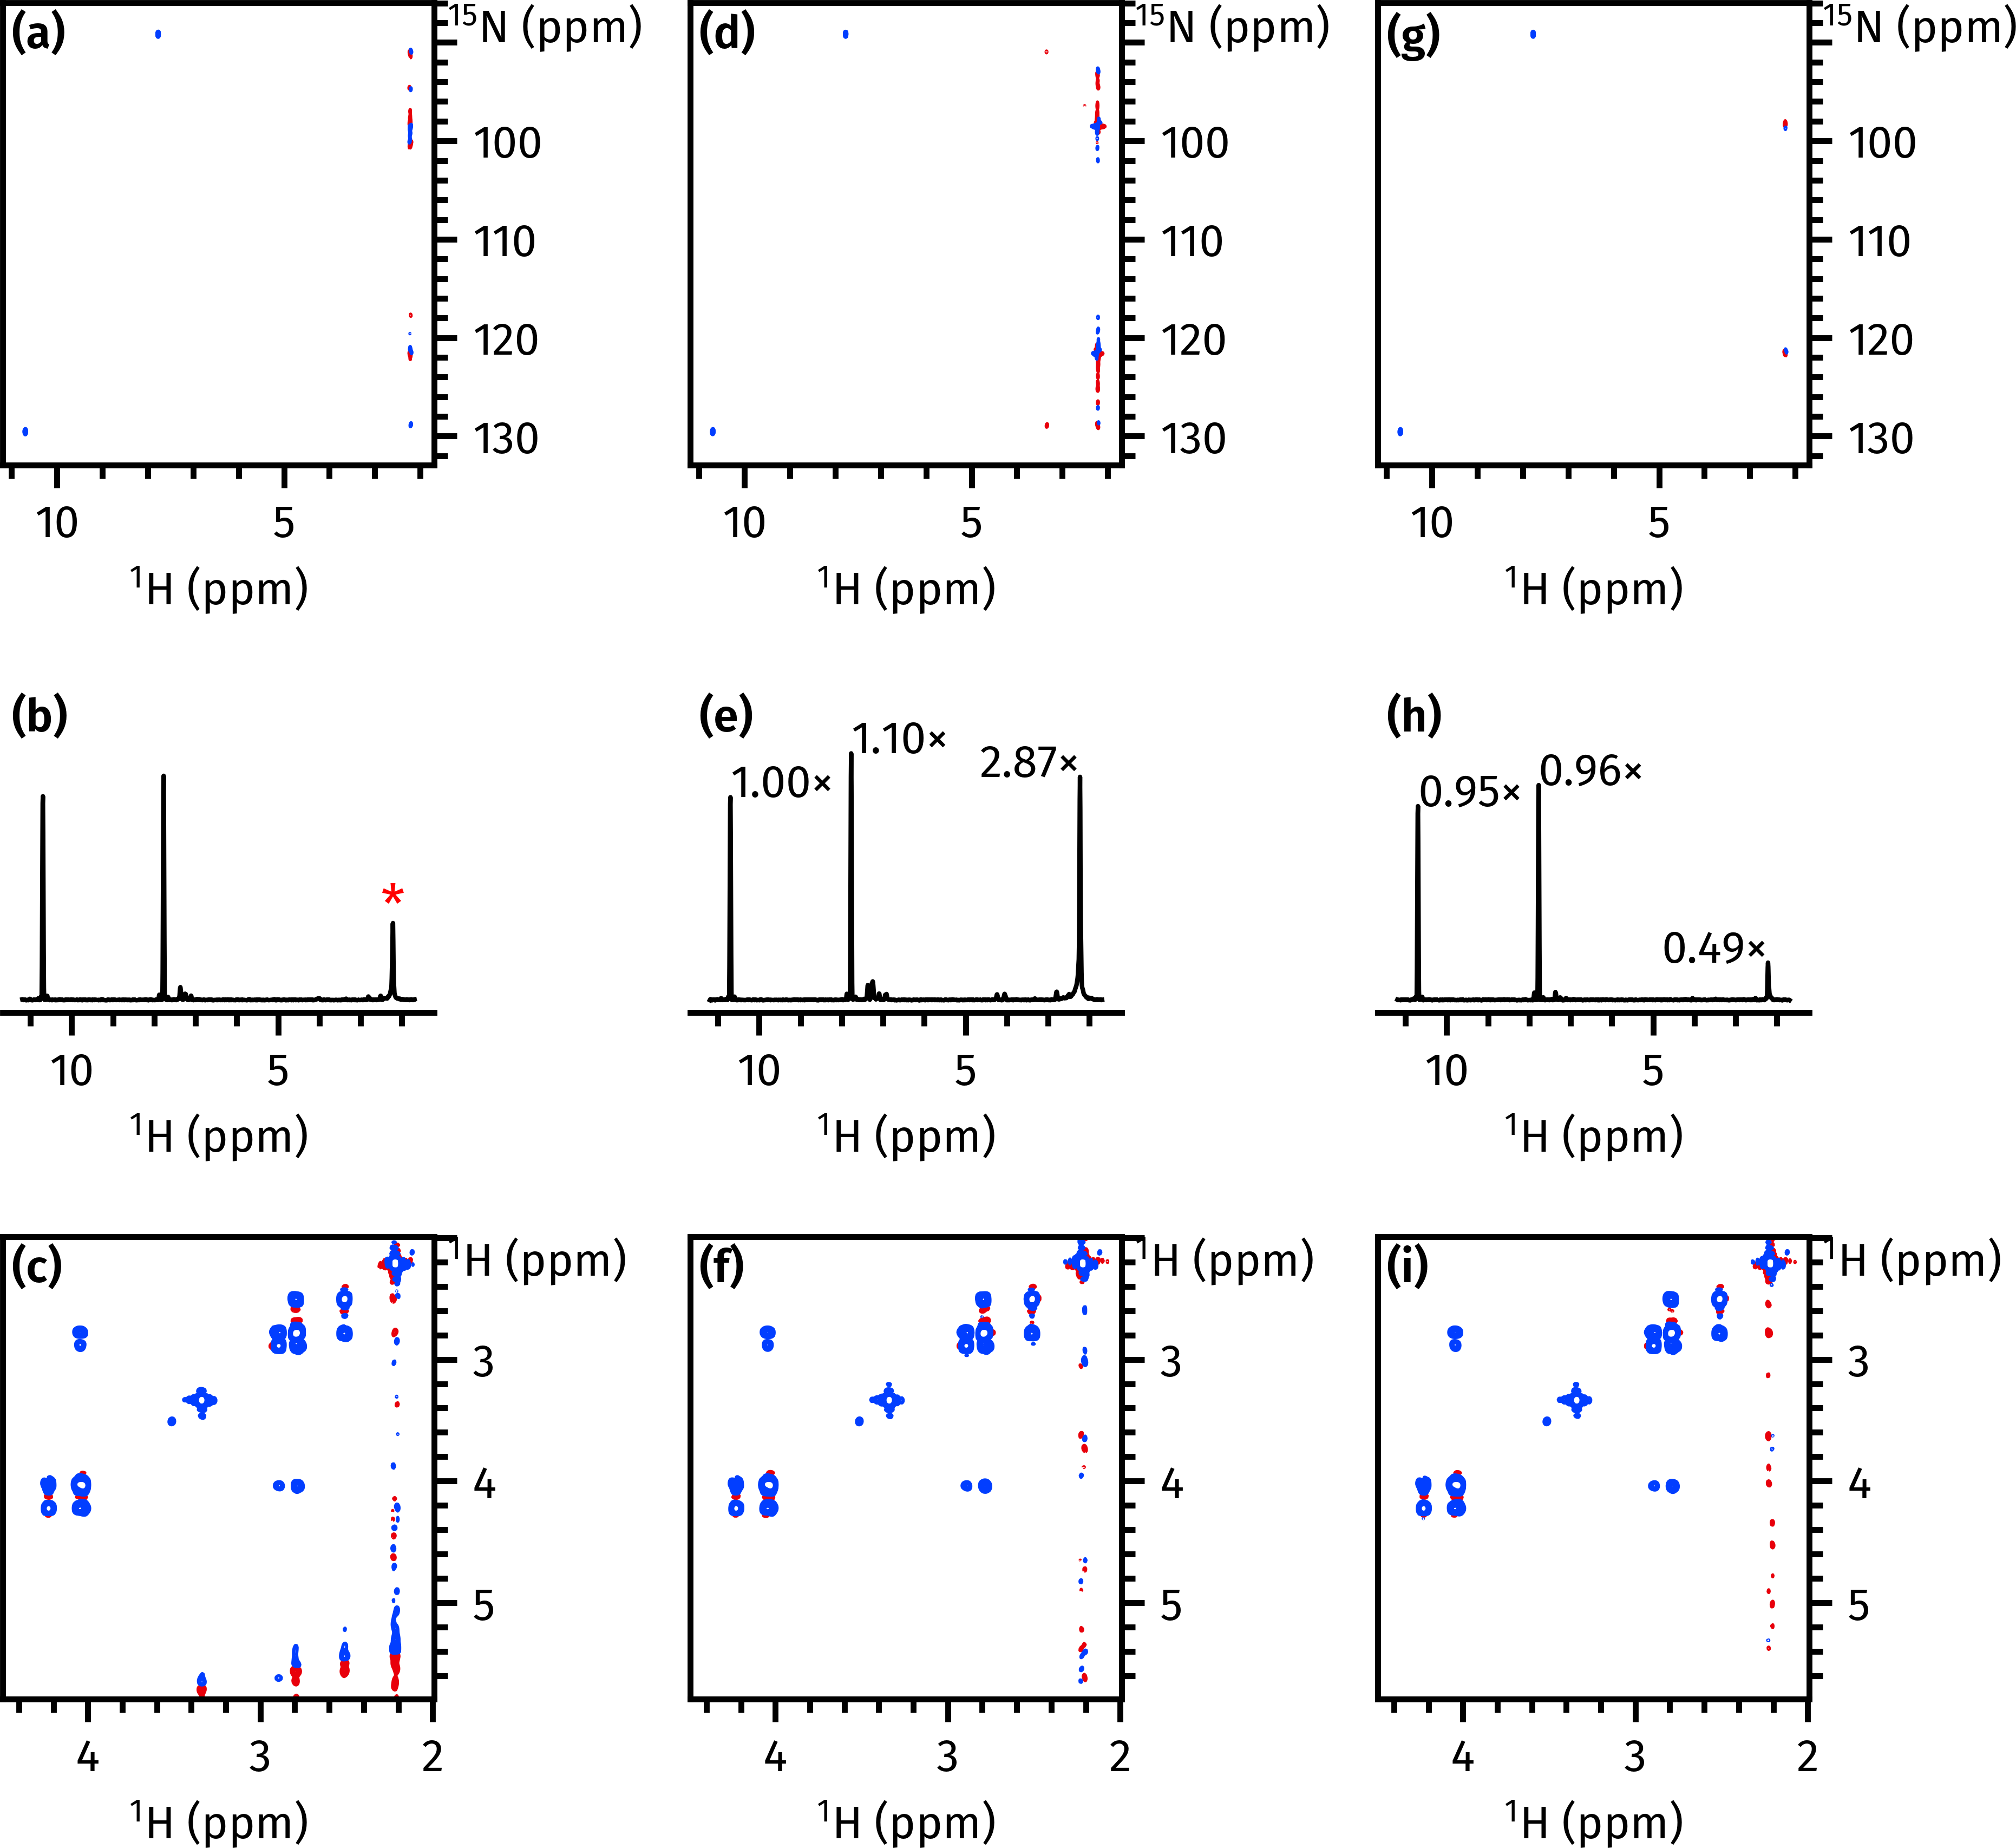
\includegraphics[draft=false]{noah/hmqc_grad.png}%
    {\phantomsubcaption\label{fig:hmqc_grad_spec_4grad_1ms_hmqc}}%
    {\phantomsubcaption\label{fig:hmqc_grad_spec_4grad_1ms_hmqcp}}%
    {\phantomsubcaption\label{fig:hmqc_grad_spec_4grad_1ms_cosy}}%
    {\phantomsubcaption\label{fig:hmqc_grad_spec_2grad_1ms_hmqc}}%
    {\phantomsubcaption\label{fig:hmqc_grad_spec_2grad_1ms_hmqcp}}%
    {\phantomsubcaption\label{fig:hmqc_grad_spec_2grad_1ms_cosy}}%
    {\phantomsubcaption\label{fig:hmqc_grad_spec_2grad_2p5ms_hmqc}}%
    {\phantomsubcaption\label{fig:hmqc_grad_spec_2grad_2p5ms_hmqcp}}%
    {\phantomsubcaption\label{fig:hmqc_grad_spec_2grad_2p5ms_cosy}}%
    \caption[Comparison of \noah{Mn,Sp,Cc} modules with different HMQC gradient schemes]{
        Comparison of HMQC and CLIP-COSY spectra obtained from \noah{Mn,Sp,Cc} supersequences, acquired using different HMQC gradient schemes.
        In the first row, the HMQC spectrum itself is shown.
        In the second row, the positive projection of the HMQC spectrum onto the $F_2$ axis is shown; the numbers indicate peak intensities with respect to the reference dataset (the left column).
        The asterisks indicate artefacts arising from bulk magnetisation which is not sufficiently dephased by the final gradient.
        In the third row, (an inset of) the CLIP-COSY spectrum is shown.
        \textbf{(\subref*{fig:hmqc_grad_spec_4grad_1ms_hmqc})--(\subref*{fig:hmqc_grad_spec_4grad_1ms_cosy})} Using the four-gradient scheme of \cref{fig:noah_hmqc_4grad}, with \qty{1}{ms} gradients.
        \textbf{(\subref*{fig:hmqc_grad_spec_2grad_1ms_hmqc})--(\subref*{fig:hmqc_grad_spec_2grad_1ms_cosy})} Using the two-gradient scheme of \cref{fig:noah_hmqc_2grad}, with \qty{1}{ms} gradients.
        \textbf{(\subref*{fig:hmqc_grad_spec_2grad_2p5ms_hmqc})--(\subref*{fig:hmqc_grad_spec_2grad_2p5ms_cosy})} Using the two-gradient scheme of \cref{fig:noah_hmqc_2grad}, with \qty{2.5}{ms} gradients.
        \datacode{7Z-200926}
    }
    \label{fig:hmqc_grad_spec}
\end{figure}

It is of some interest to check whether such a long gradient is truly required.
I therefore ran the two-gradient HMQC experiment with a series of gradient durations from \qty{1}{\ms} to \qty{2.5}{\ms}; the signal and artefact intensities in each of these experiments are plotted in \cref{fig:hmqc_cnst16}.
Generally, there is little variation in the intensities of the two desired peaks.
The artefact intensity is more erratic, which possibly reflects the fact that gradient dephasing varies sinusoidally with the gradient duration $\tau$ due to the spatial integral
\begin{equation}
    \label{eq:gradient_dephasing}
    \frac{1}{L} \int_{-L/2}^{L/2} \exp(\mi \gamma Gz\tau)\,\mathrm{d}z = \frac{\sin(\gamma G L\tau/2)}{\gamma GL\tau/2},
\end{equation}
where $L$ is the sample length and $G$ the gradient amplitude (see also \cref{eq:density_operator_integration}).
Nevertheless, there is a clear decrease in the signal intensity as the gradient duration increases, which (at least in these datasets) is greatest with \qty{2.5}{\ms} gradients.
Since the signal intensity is not affected much, I deemed this to be a perfectly suitable value.

\begin{figure}[!ht]
    \centering
    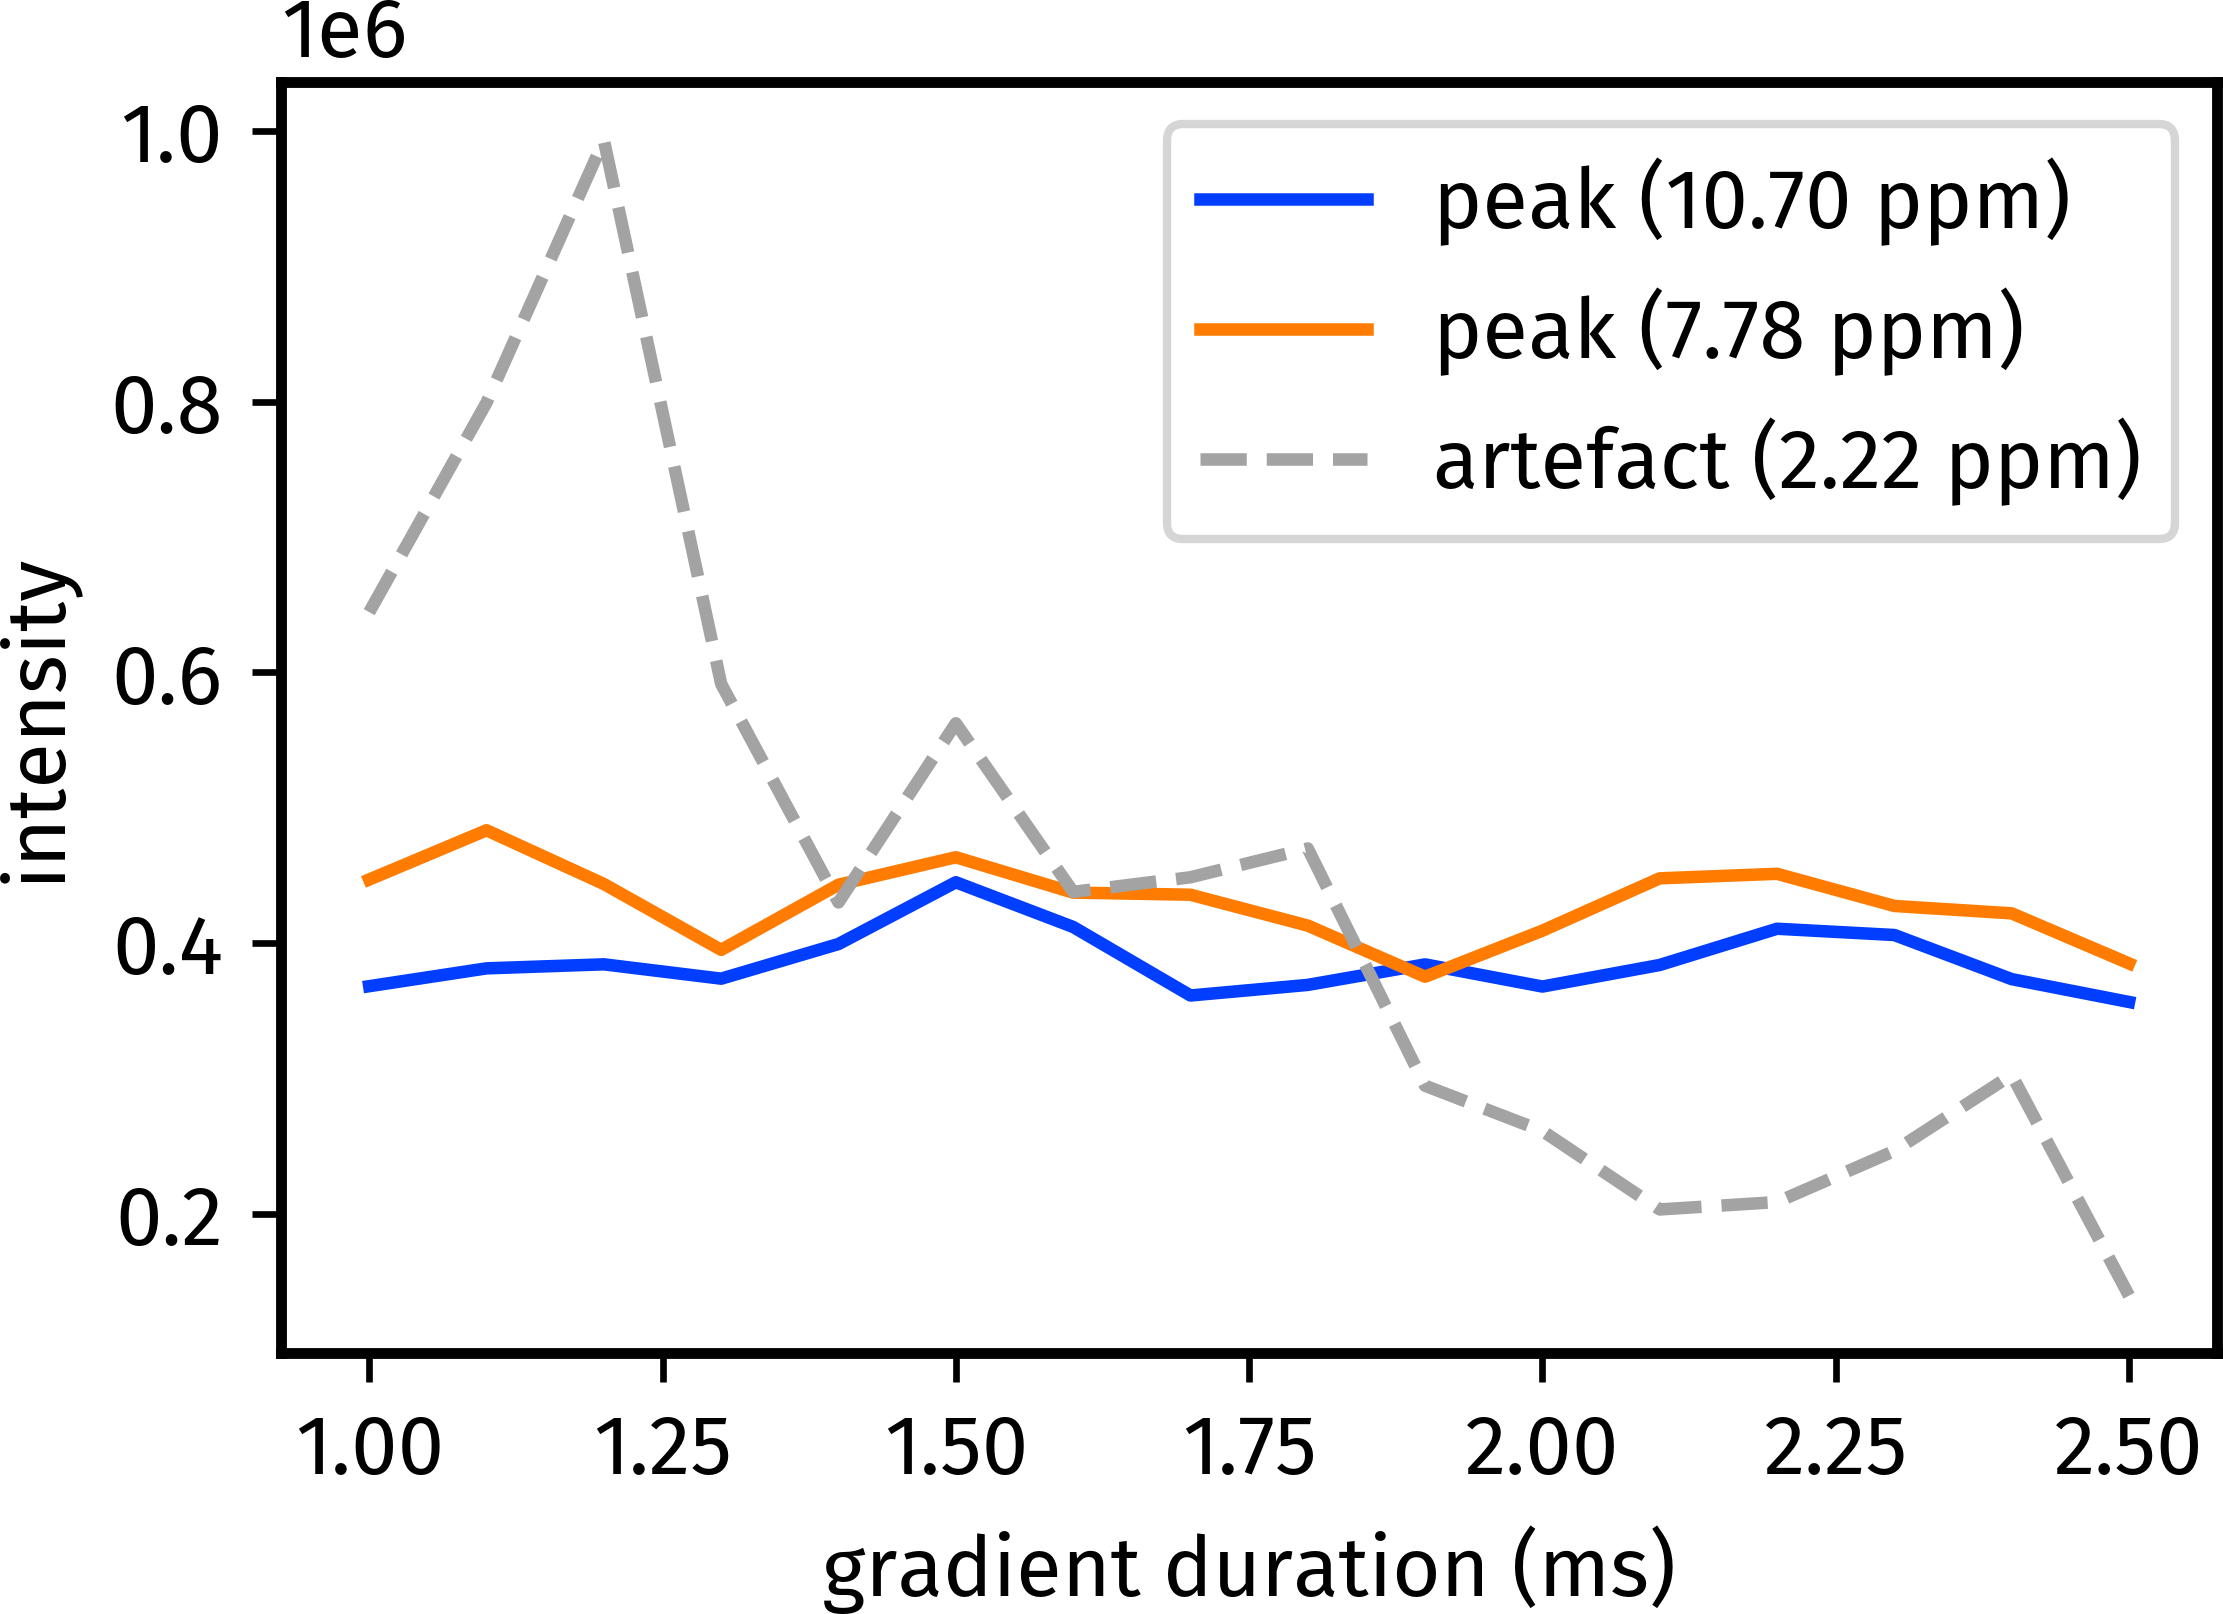
\includegraphics[draft=false]{noah/hmqc_cnst16_scan.png}%
    \caption[Variation of HMQC signal and artefact intensity with CTP gradient duration]{
        Variation of HMQC signal and artefact intensity with CTP gradient duration.
        \datacode{7Z-200926}
    }
    \label{fig:hmqc_cnst16}
\end{figure}



\subsubsection{$\symbfit{k}$- and SW-scaling}

\proton{}--\nitrogen{} spectra of small molecules are often relatively sparse in the indirect dimension, and do not typically need to be acquired with the same resolution as a \proton{}--\carbon{} experiment.
However, if these experiments were to be combined together within a supersequence, it is not ordinarily possible to toggle the resolution of each module individually.
One way of circumventing this issue is to decrease the frequency with which the \nitrogen{} $t_1$ duration is incremented in the pulse programme: this was first proposed by Parella et al.\ in the context of time-shared NMR\autocite{PerezTrujillo2007MRC,Parella2010CMR}, and in this thesis is called `$k$-scaling'.
This means that each $t_1$ increment is acquired several times before $t_1$ is incremented; effectively leading to $k$ times fewer $t_1$ increments, but with each increment having $k$ times the number of scans (after the data have been combined).
An alternative is to simply increase the spectral width of the \nitrogen{} module (which is encoded as the \texttt{CNST40} parameter in GENESIS).

\begin{figure}[!ht]
    \centering
    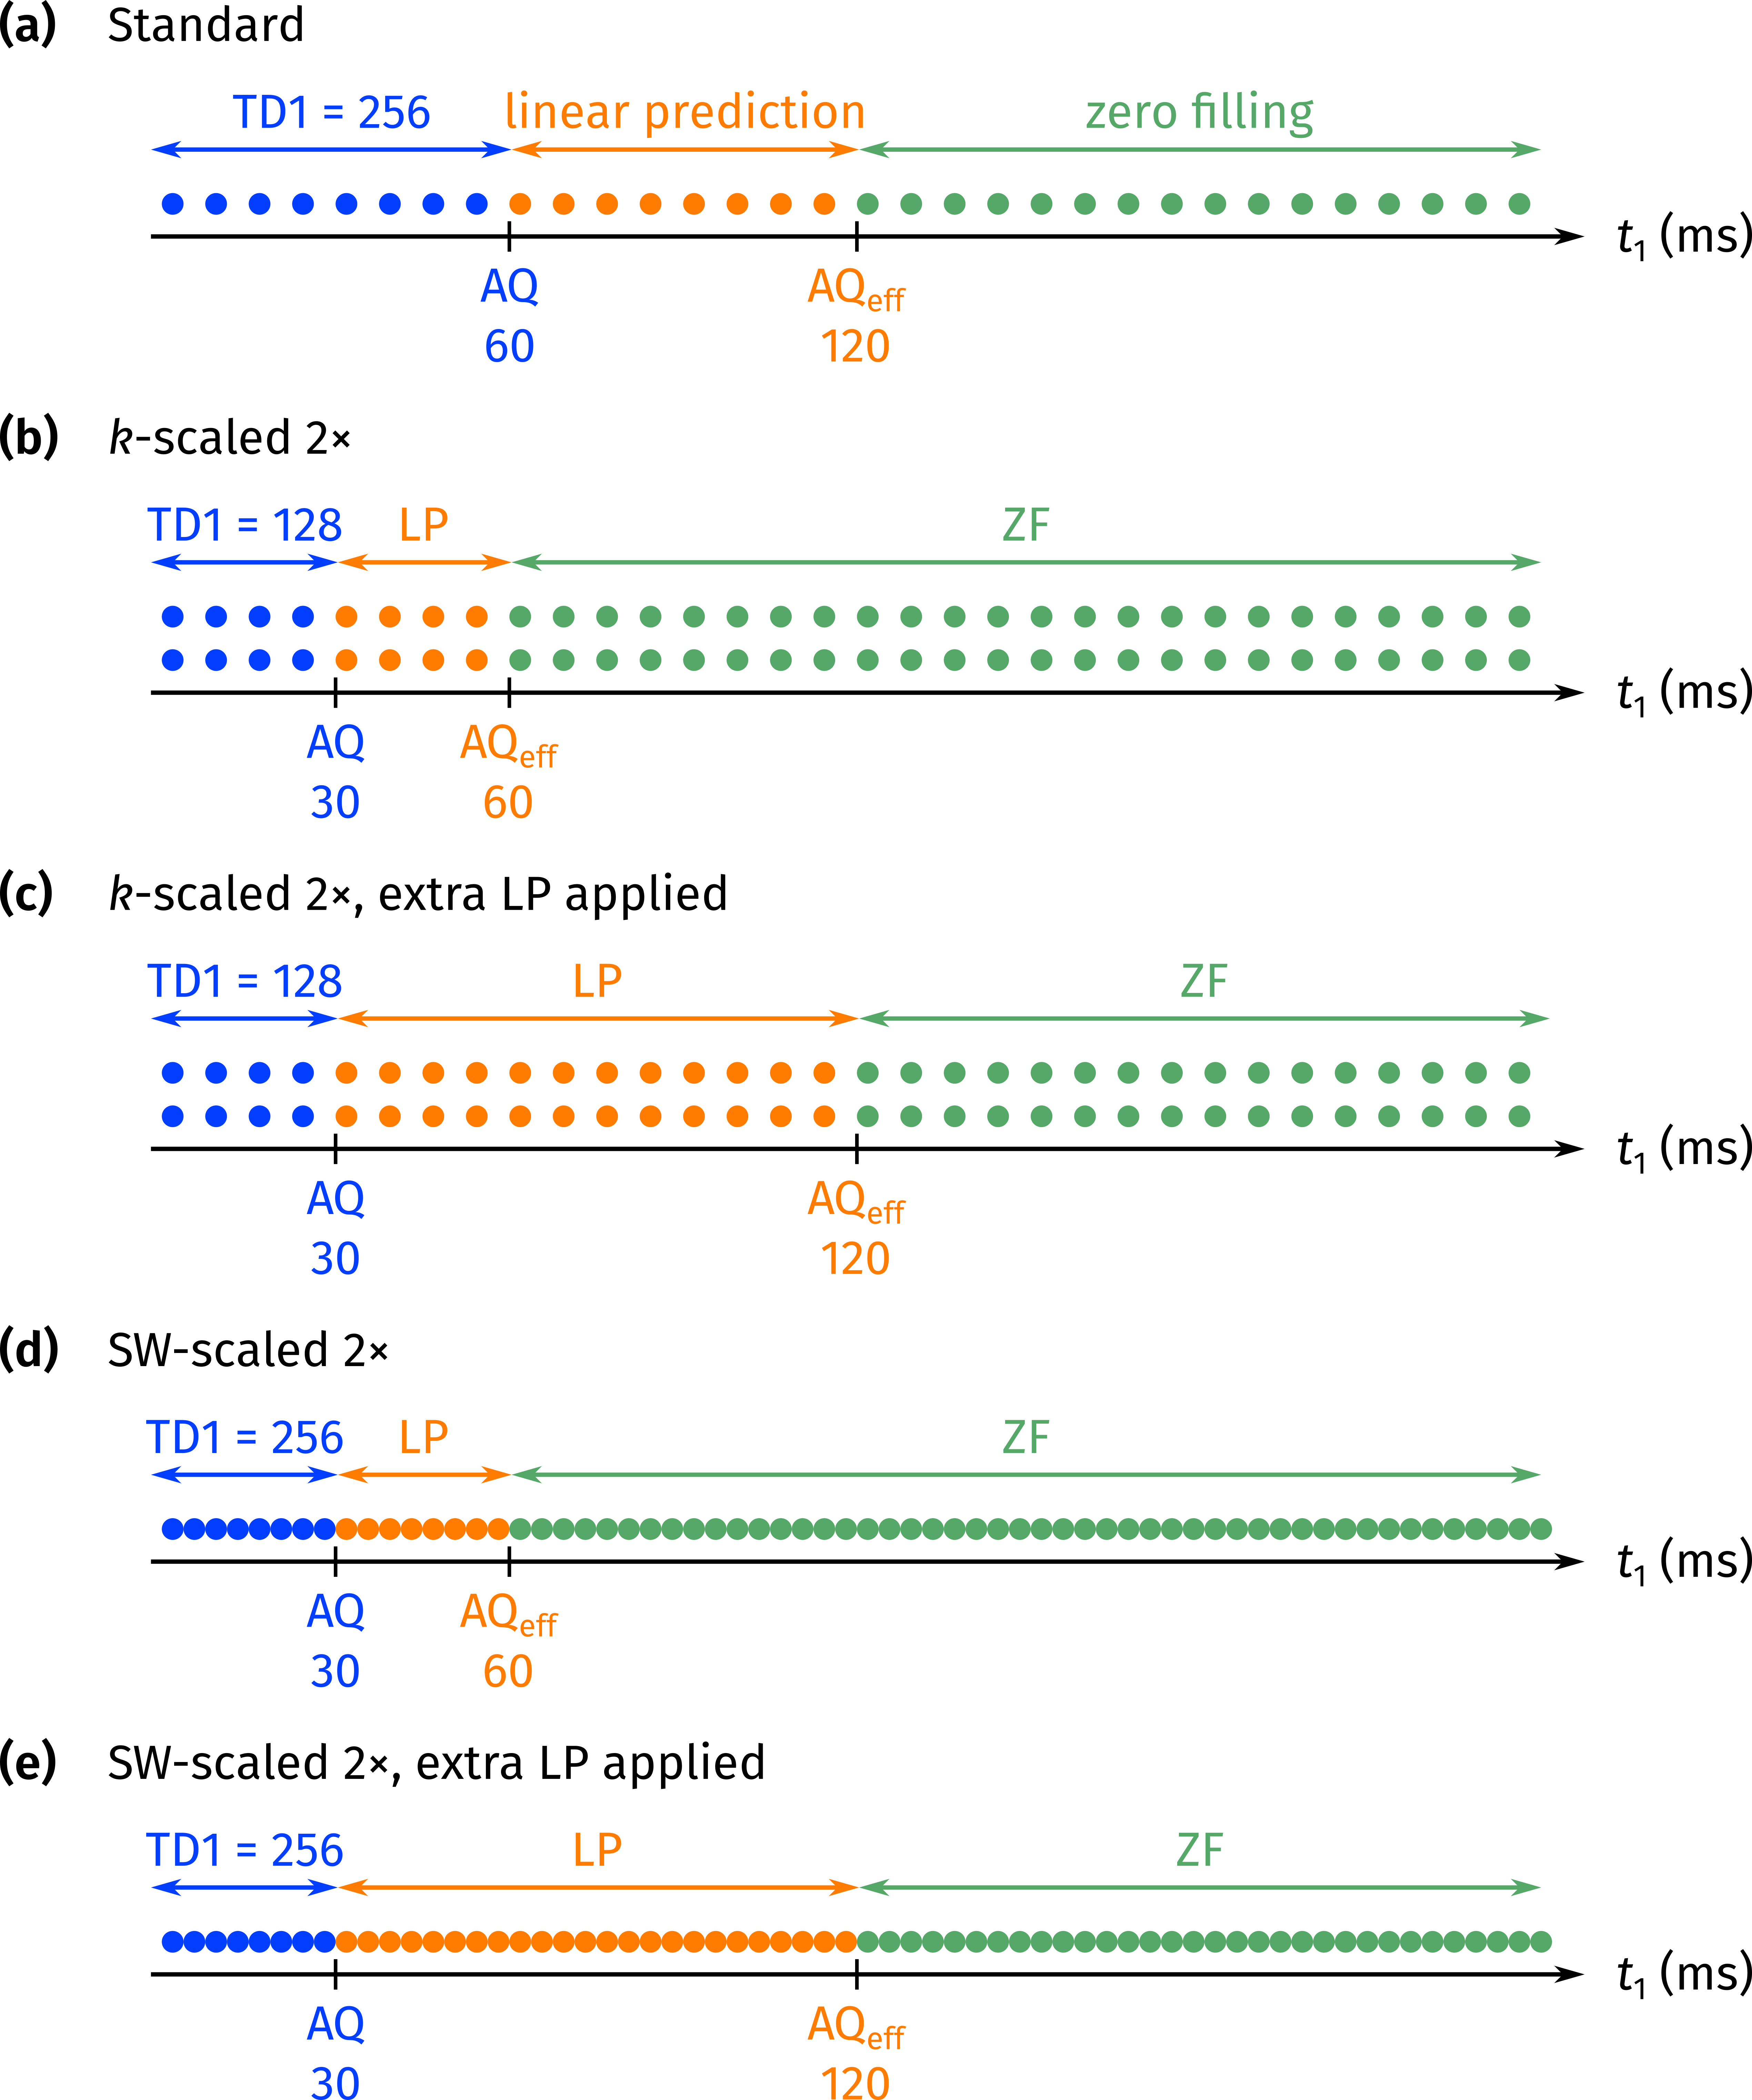
\includegraphics[draft=false]{noah/n15_t1_diagram.png}%
    {\phantomsubcaption\label{fig:n15_t1_normal}}%
    {\phantomsubcaption\label{fig:n15_t1_k}}%
    {\phantomsubcaption\label{fig:n15_t1_k_lp}}%
    {\phantomsubcaption\label{fig:n15_t1_sw}}%
    {\phantomsubcaption\label{fig:n15_t1_sw_lp}}%
    \caption[Pictorial representation of $k$- and SW-scaling in NOAH \nitrogen{} modules]{
        Pictorial representation of $k$- and SW-scaling in NOAH \nitrogen{} modules.
        Each blue dot represents 32 $t_1$ increments physically acquired as part of the experiment; the experimental time is proportional to the number of blue dots, and is constant across all of these experiments.
        Orange dots represent 32 $t_1$ increments obtained through forward linear prediction, and green dots represent zeroes.
        \textbf{(\subref*{fig:n15_t1_normal})} The default experiment.
        \textbf{(\subref*{fig:n15_t1_k})--(\subref*{fig:n15_t1_k_lp})} $k$-scaled experiment, without and with extra linear processing to restore the original value of $\AQeff$.
        \textbf{(\subref*{fig:n15_t1_sw})--(\subref*{fig:n15_t1_sw_lp})} SW-scaled experiment, without and with extra linear processing to restore the original value of $\AQeff$.
    }
    \label{fig:n15_t1}
\end{figure}

\Cref{fig:n15_t1} illustrates all of these possibilities in detail.
In a `typical' NOAH supersequence (\cref{fig:n15_t1_normal}), 256 $t_1$ increments would be recorded (corresponding to the eight blue dots);
for the gramicidin sample used here, the largest value of $t_1$ (denoted as $\AQ$) is around \qty{60}{\ms}.
The default TopSpin processing routine for 2D NMR applies forward linear prediction (LP)\autocite{Ni1986JMR,Tirendi1989JMR,Led1991CR,Koehl1999PNMRS} in the indirect dimension, such as to double the number of points: the data points obtained through LP are indicated by orange dots.
This leads to an \textit{effective} AQ which is twice as large, denoted as $\AQeff$.
Finally, zero filling (ZF) is applied to increase the digital resolution to a given value, as represented by the green dots.

In the $k$-scaled spectrum, both AQ (and thus $\AQeff$) are halved, in return for a doubling of the number of scans (\cref{fig:n15_t1_k}).
The resolution in the indirect dimension is proportional to $\AQeff$; thus, this also corresponds to a $2\times$ decrease in resolution.
However, this can be counteracted through the use of extra linear prediction (\cref{fig:n15_t1_k_lp}) to extend $\AQeff$ back to its original value.
The SW-scaled spectra (\cref{fig:n15_t1_sw,fig:n15_t1_sw_lp}) are almost entirely equivalent to the $k$-scaled spectra in terms of their effect on AQ and $\AQeff$, except that the sampling schedule is very slightly modified.

\Cref{fig:hmqc_scale} shows the effects of performing $k$- or SW-scaling on the \nitrogen{} HMQC module (without any extra linear prediction beyond the default).
In this case, these scaling procedures can in fact can lead to significant gains in SNR (as measured by peak heights), with up to $2.6\times$ improvements being observed at the extreme of 8-fold $k$- or SW-scaling.
This likely arises because the $J_{\ch{HH}}$ modulation in the indirect dimension (visible in the standard spectrum, \cref{fig:hmqc_scale_std1}) is no longer being resolved: the largest gains are attained for the peak at \qty{123}{\ppm}, where this modulation is especially prominent.

\begin{figure}[!htbp]
    \centering
    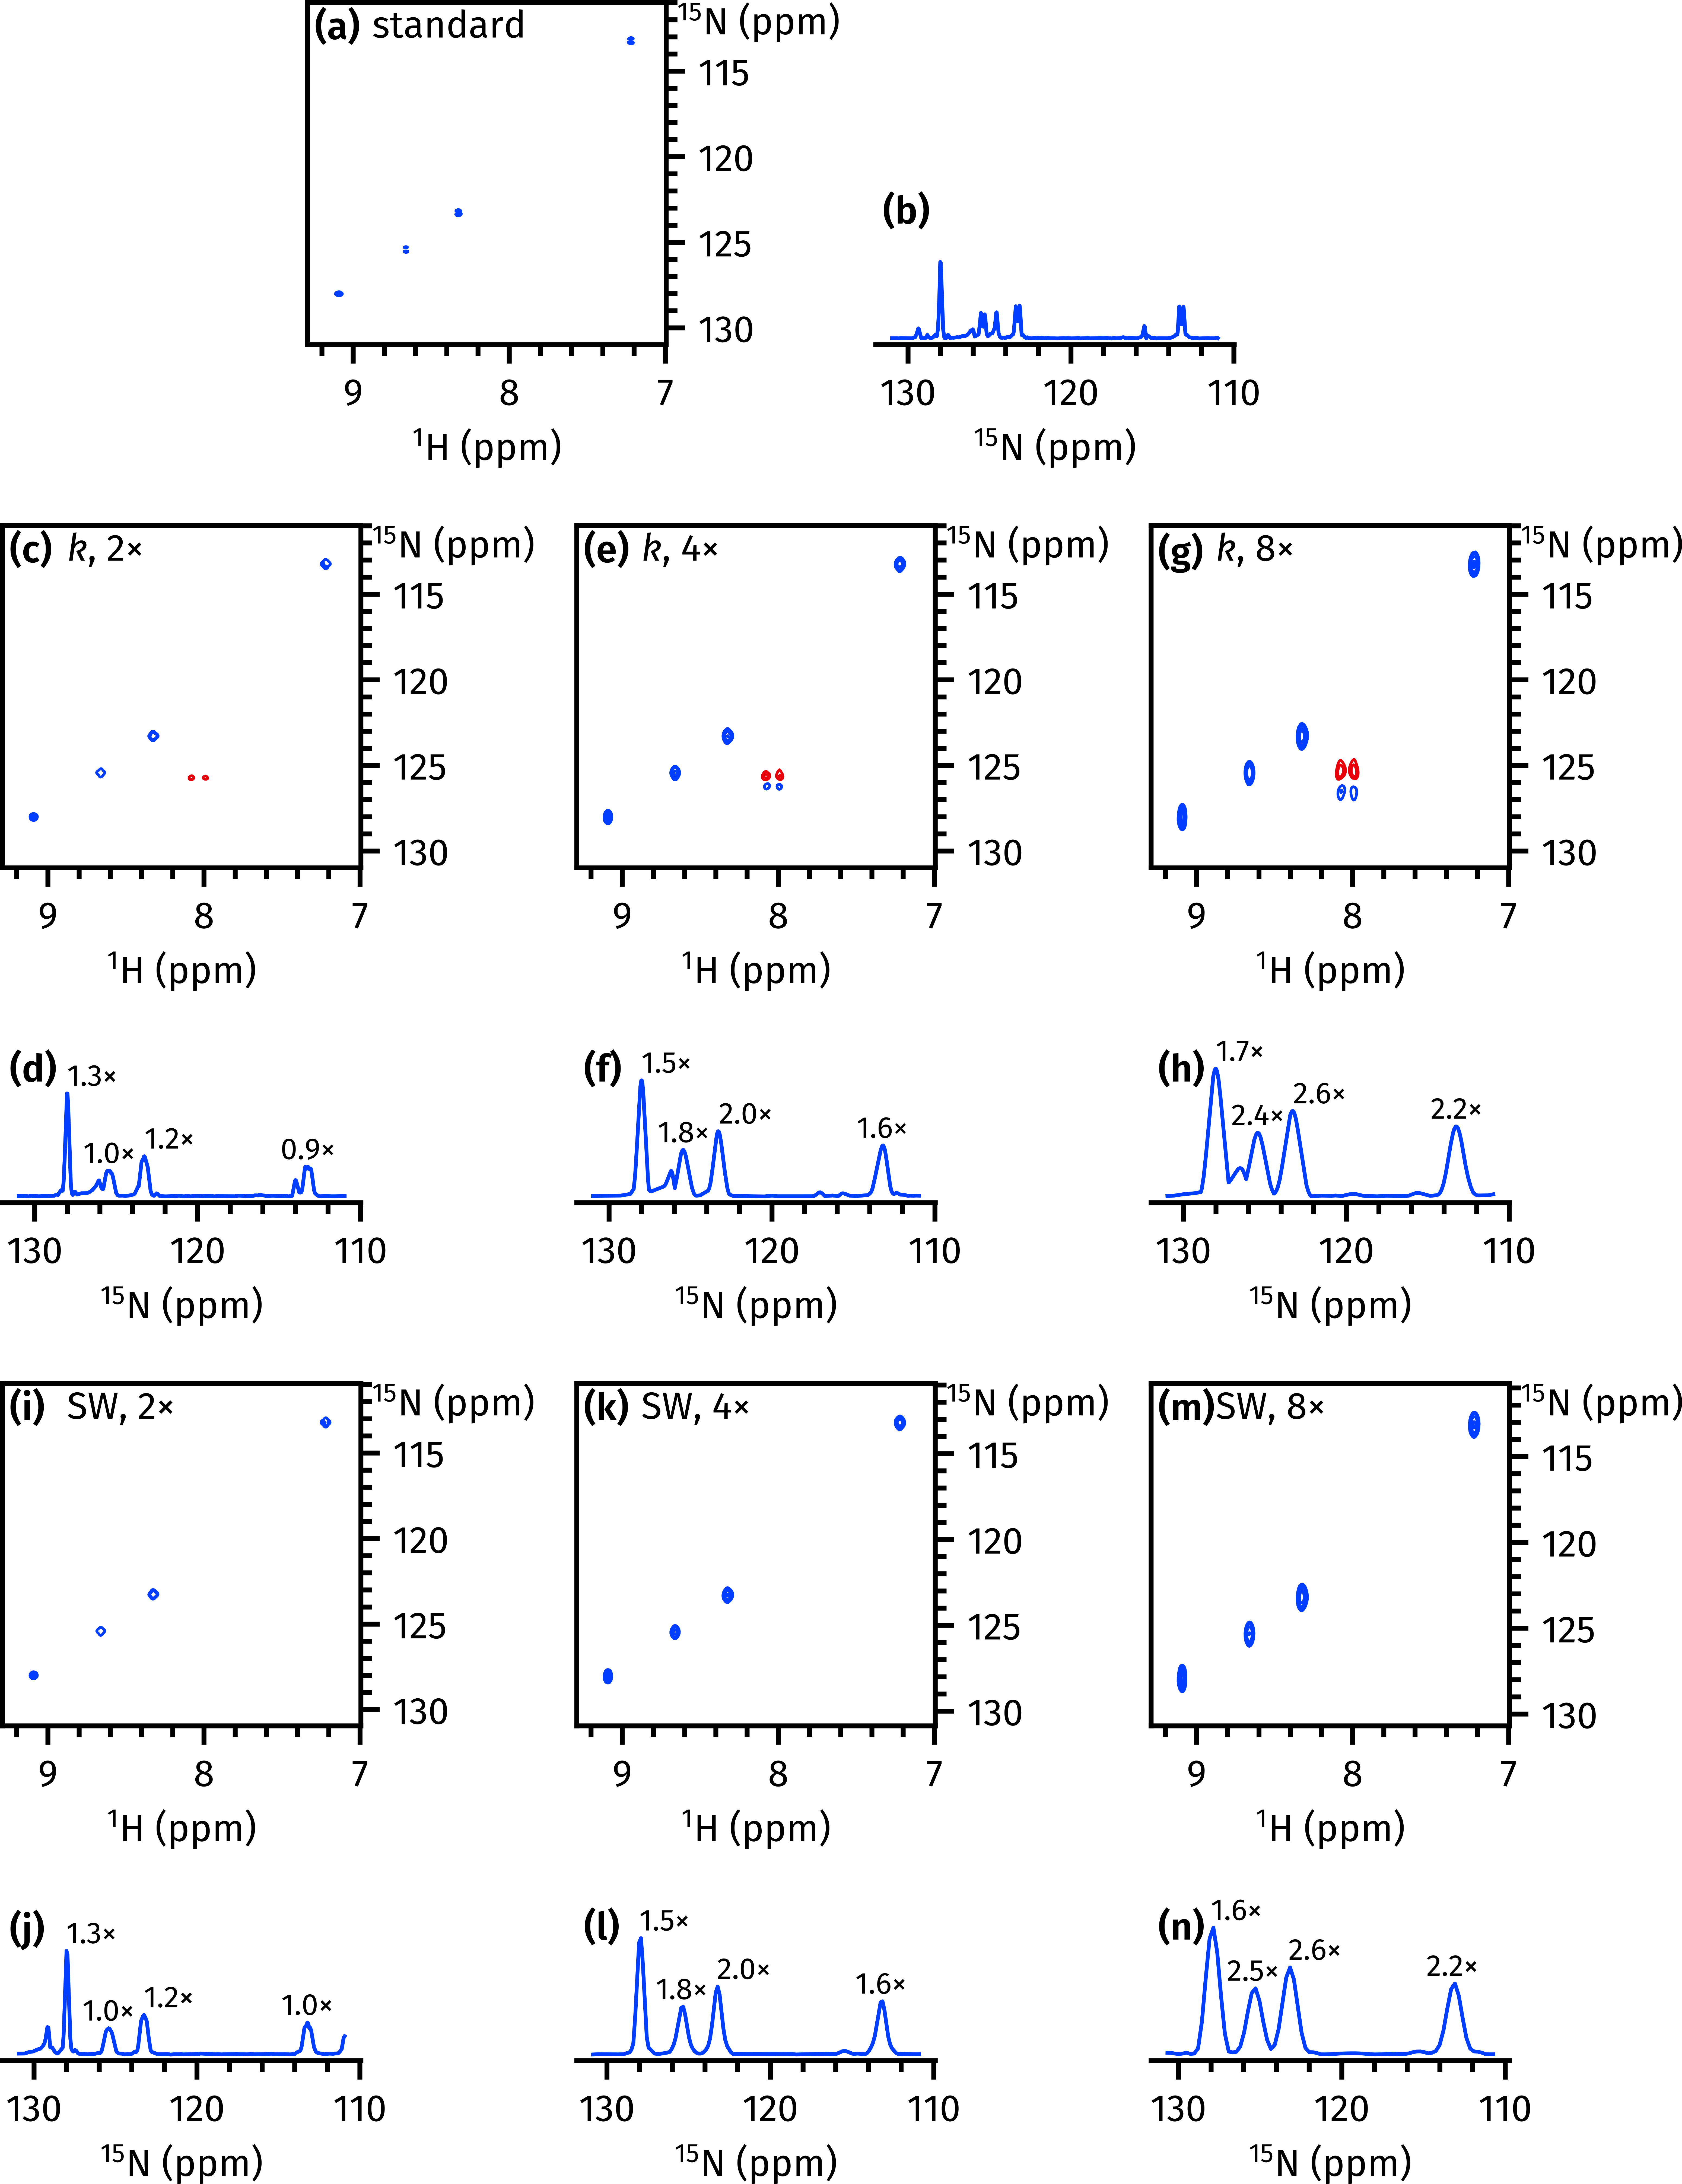
\includegraphics[draft=false]{noah/hmqc_scale.png}%
    {\phantomsubcaption\label{fig:hmqc_scale_std2}}%
    {\phantomsubcaption\label{fig:hmqc_scale_std1}}%
    {\phantomsubcaption\label{fig:hmqc_scale_k22}}%
    {\phantomsubcaption\label{fig:hmqc_scale_k21}}%
    {\phantomsubcaption\label{fig:hmqc_scale_k42}}%
    {\phantomsubcaption\label{fig:hmqc_scale_k41}}%
    {\phantomsubcaption\label{fig:hmqc_scale_k82}}%
    {\phantomsubcaption\label{fig:hmqc_scale_k81}}%
    {\phantomsubcaption\label{fig:hmqc_scale_sw22}}%
    {\phantomsubcaption\label{fig:hmqc_scale_sw21}}%
    {\phantomsubcaption\label{fig:hmqc_scale_sw42}}%
    {\phantomsubcaption\label{fig:hmqc_scale_sw41}}%
    {\phantomsubcaption\label{fig:hmqc_scale_sw82}}%
    {\phantomsubcaption\label{fig:hmqc_scale_sw81}}%
    \caption[Effects of $k$- and SW-scaling on NOAH HMQC spectrum]{
        Effects of $k$- and SW-scaling on NOAH HMQC spectrum (taken from \noah{Mn,Sp,Cc} supersequences).
        Each HMQC spectrum is shown together with a positive projection onto the $F_1$ axis.
        The relative SNR of each peak, with respect to the standard spectrum, is indicated on each of the other projections.
        \textbf{(\subref*{fig:hmqc_scale_std2})--(\subref*{fig:hmqc_scale_std1})} Standard spectrum.
        \textbf{(\subref*{fig:hmqc_scale_k22})--(\subref*{fig:hmqc_scale_k81})} $k$-scaled spectra.
        \textbf{(\subref*{fig:hmqc_scale_sw22})--(\subref*{fig:hmqc_scale_sw81})} SW-scaled spectra.
        \datacode{7G-210310}
    }
    \label{fig:hmqc_scale}
\end{figure}

The effect of adding extra linear prediction is shown in \cref{fig:hmqc_scale_lp}.
In general, the combination of scaling plus LP leads to improvements in spectral SNR of up to $6\times$.
However, this is accompanied by distortions in the $F_1$ multiplet structure, especially for the $k$-scaled spectra (\cref{fig:hmqc_scale_lp_k22,fig:hmqc_scale_lp_k21,fig:hmqc_scale_lp_k42,fig:hmqc_scale_lp_k41,fig:hmqc_scale_lp_k82,fig:hmqc_scale_lp_k81}): it is possible that the corresponding SW-scaled spectra are not so heavily distorted because there are more data points to extrapolate from.

However, caution should be exercised when interpreting these results.
Although this improvement in SNR is genuine, it is not necessarily the case that this represents a true improvement in \textit{detection sensitivity}: in other words, processing techniques such as LP (and to some extent, NUS) do not always allow for better discrimination between signal and noise.\autocite{Donoho1990PNASUSA,Stern2002JACS}%
\footnote{In recent years, this issue has been investigated more thoroughly in the context of NUS.\autocite{Palmer2015JPCB}}
Further tests would need to be done on more dilute samples\footnote{Or, perhaps, less sensitive instruments---although the \qty{700}{\MHz} cryoprobe used here was the only option for these supersequences.} to ascertain the benefits of the scaling-plus-LP routine on spectra with less intrinsic SNR.

\begin{figure}[!htbp]
    \centering
    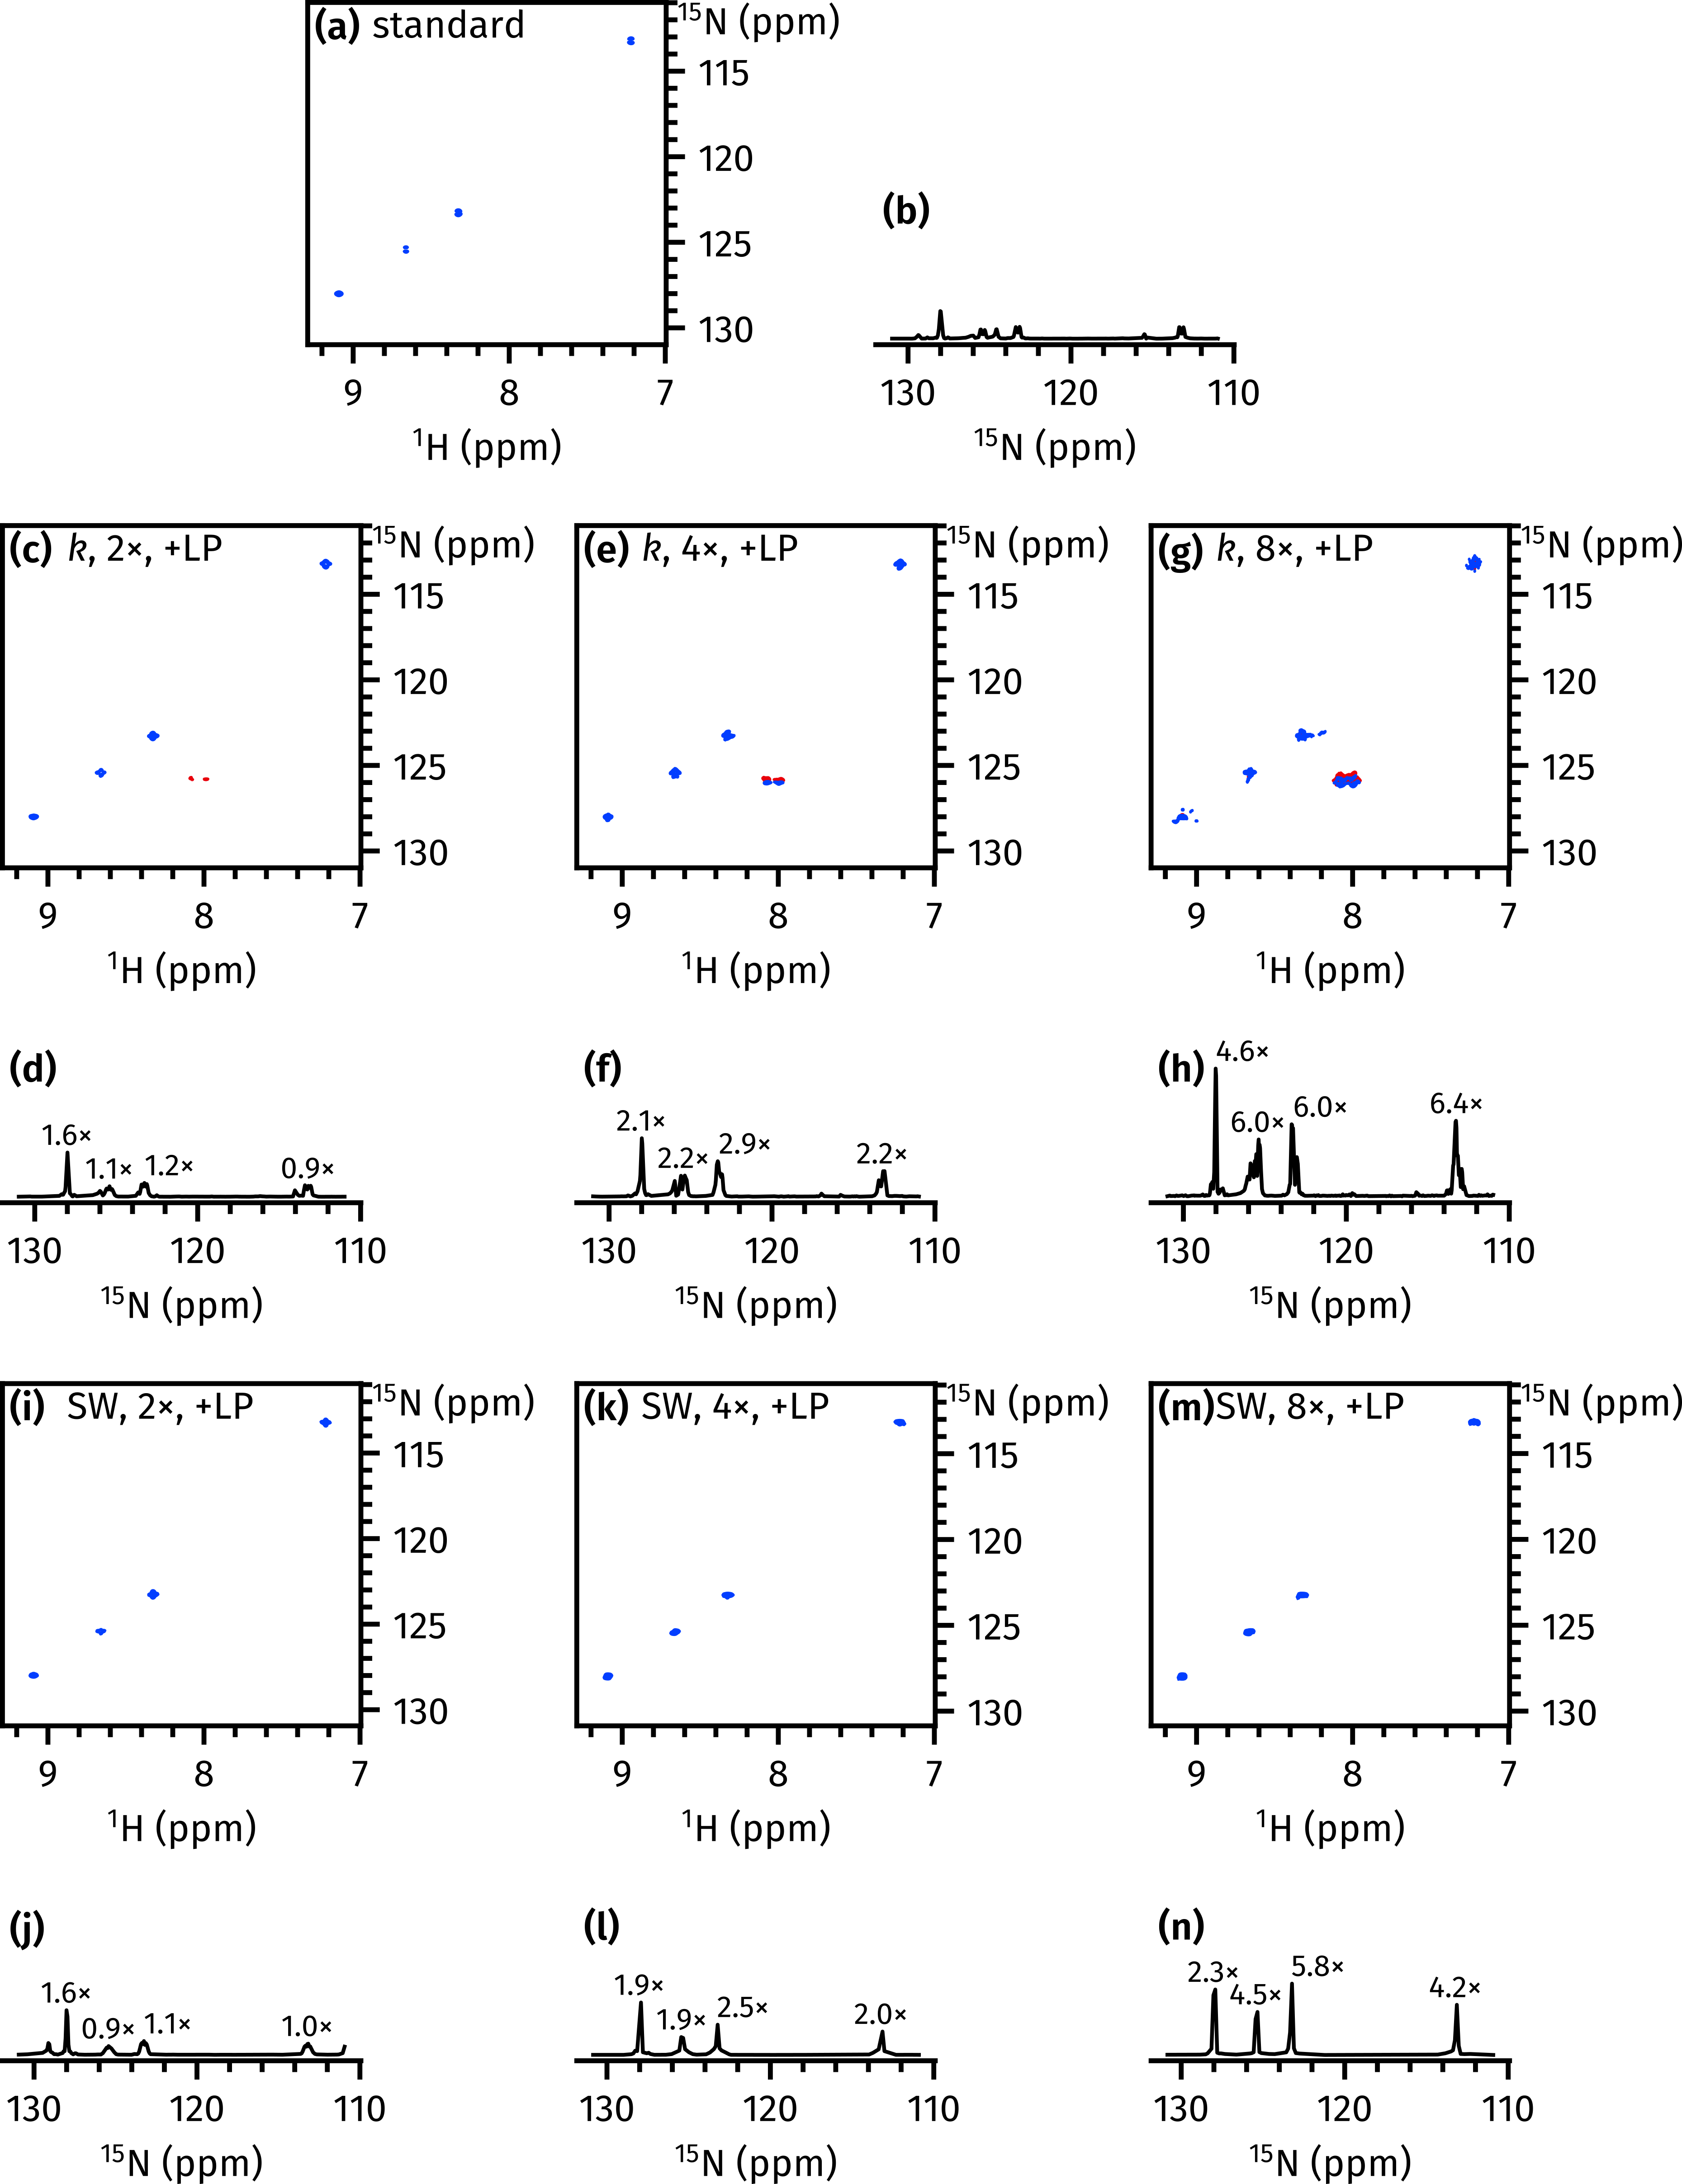
\includegraphics[draft=false]{noah/hmqc_scale_lp.png}%
    {\phantomsubcaption\label{fig:hmqc_scale_lp_std2}}%
    {\phantomsubcaption\label{fig:hmqc_scale_lp_std1}}%
    {\phantomsubcaption\label{fig:hmqc_scale_lp_k22}}%
    {\phantomsubcaption\label{fig:hmqc_scale_lp_k21}}%
    {\phantomsubcaption\label{fig:hmqc_scale_lp_k42}}%
    {\phantomsubcaption\label{fig:hmqc_scale_lp_k41}}%
    {\phantomsubcaption\label{fig:hmqc_scale_lp_k82}}%
    {\phantomsubcaption\label{fig:hmqc_scale_lp_k81}}%
    {\phantomsubcaption\label{fig:hmqc_scale_lp_sw22}}%
    {\phantomsubcaption\label{fig:hmqc_scale_lp_sw21}}%
    {\phantomsubcaption\label{fig:hmqc_scale_lp_sw42}}%
    {\phantomsubcaption\label{fig:hmqc_scale_lp_sw41}}%
    {\phantomsubcaption\label{fig:hmqc_scale_lp_sw82}}%
    {\phantomsubcaption\label{fig:hmqc_scale_lp_sw81}}%
    \caption[Effects of $k$- and SW-scaling on NOAH HMQC spectrum with extra linear prediction]{
        The same as in \cref{fig:hmqc_scale}, but with extra linear prediction applied to all scaled spectra to bring $\AQeff$ up to its original value in the standard spectrum.
        Linear prediction of $k$ times more points leads to a $\sqrt{k}$ increase in noise; to account for this, all spectra are plotted with the same noise level.
        \textbf{(\subref*{fig:hmqc_scale_lp_std2})--(\subref*{fig:hmqc_scale_lp_std1})} Standard spectrum.
        \textbf{(\subref*{fig:hmqc_scale_lp_k22})--(\subref*{fig:hmqc_scale_lp_k81})} $k$-scaled spectra.
        \textbf{(\subref*{fig:hmqc_scale_lp_sw22})--(\subref*{fig:hmqc_scale_lp_sw81})} SW-scaled spectra.
        \datacode{7G-210310}
    }
    \label{fig:hmqc_scale_lp}
\end{figure}

\subsection{HSQC-TOCSY}
\label{subsec:noah__hsqctocsy}

HSQC + DIPSI + HSQC combos

Extension to HSQC-TOCSY

Cite ASAP work (Luy)

\subsection{HSQC-COSY}
\label{subsec:noah__hsqccosy}

One downside of the HSQC-TOCSY experiment discussed in the previous section is the (largely) indiscriminate transfer of magnetisation effected by the DIPSI mixing.
It is difficult to determine how many transfer steps give rise to each peak, unless several HSQC-TOCSY spectra with different mixing times are recorded, which is a time-consuming process.%
\footnote{Of course, as per the previous section, this could be done in a NOAH supersequence where each HSQC-TOCSY spectrum is assigned a fraction of the \magn{C} magnetisation. However, one must be wary of stretching the same magnetisation pool too thinly between many different modules: the resulting decrease in signal intensity may lead to a crossing into the sensitivity-limited regime.}

For unambiguous spectral assignment, it can be preferable to have a mixing process which only effects coherence transfer across a single coupling: this can be described as an HSQC-COSY experiment.
Similar experiments, including the H2BC\autocite{Nyberg2005JACS,Nyberg2005MRC}, 2BOB/H2OBC\autocite{Kupce2017MRC}, and HMQC-COSY\autocite{Hu2011JBNMR} have previously been reported: the 2BOB experiment in particular has previously been incorporated in NOAH supersequences\autocite{Kupce2019JMR}.
These often use constant-time techniques in order to remove $\nJ{HH}$ splittings and minimise linewidths in the indirect dimension; however, the drawback of this approach is that peak \textit{amplitudes} are modulated by $\nJ{HH}$.
Furthermore, it is not generally possible to obtain absorption-mode lineshapes for all peaks in the spectrum: typically the `direct' responses are in-phase absorption, and `indirect' responses antiphase dispersion.
(Here, the terms in-phase and antiphase are used with respect to $\nJ{HH}$; specifically, for the indirect peaks, this refers to the `active' coupling over which the coherence was transferred).


\subsubsection{HSQC-CLIP-COSY}

\begin{figure}[!ht]
    \centering
    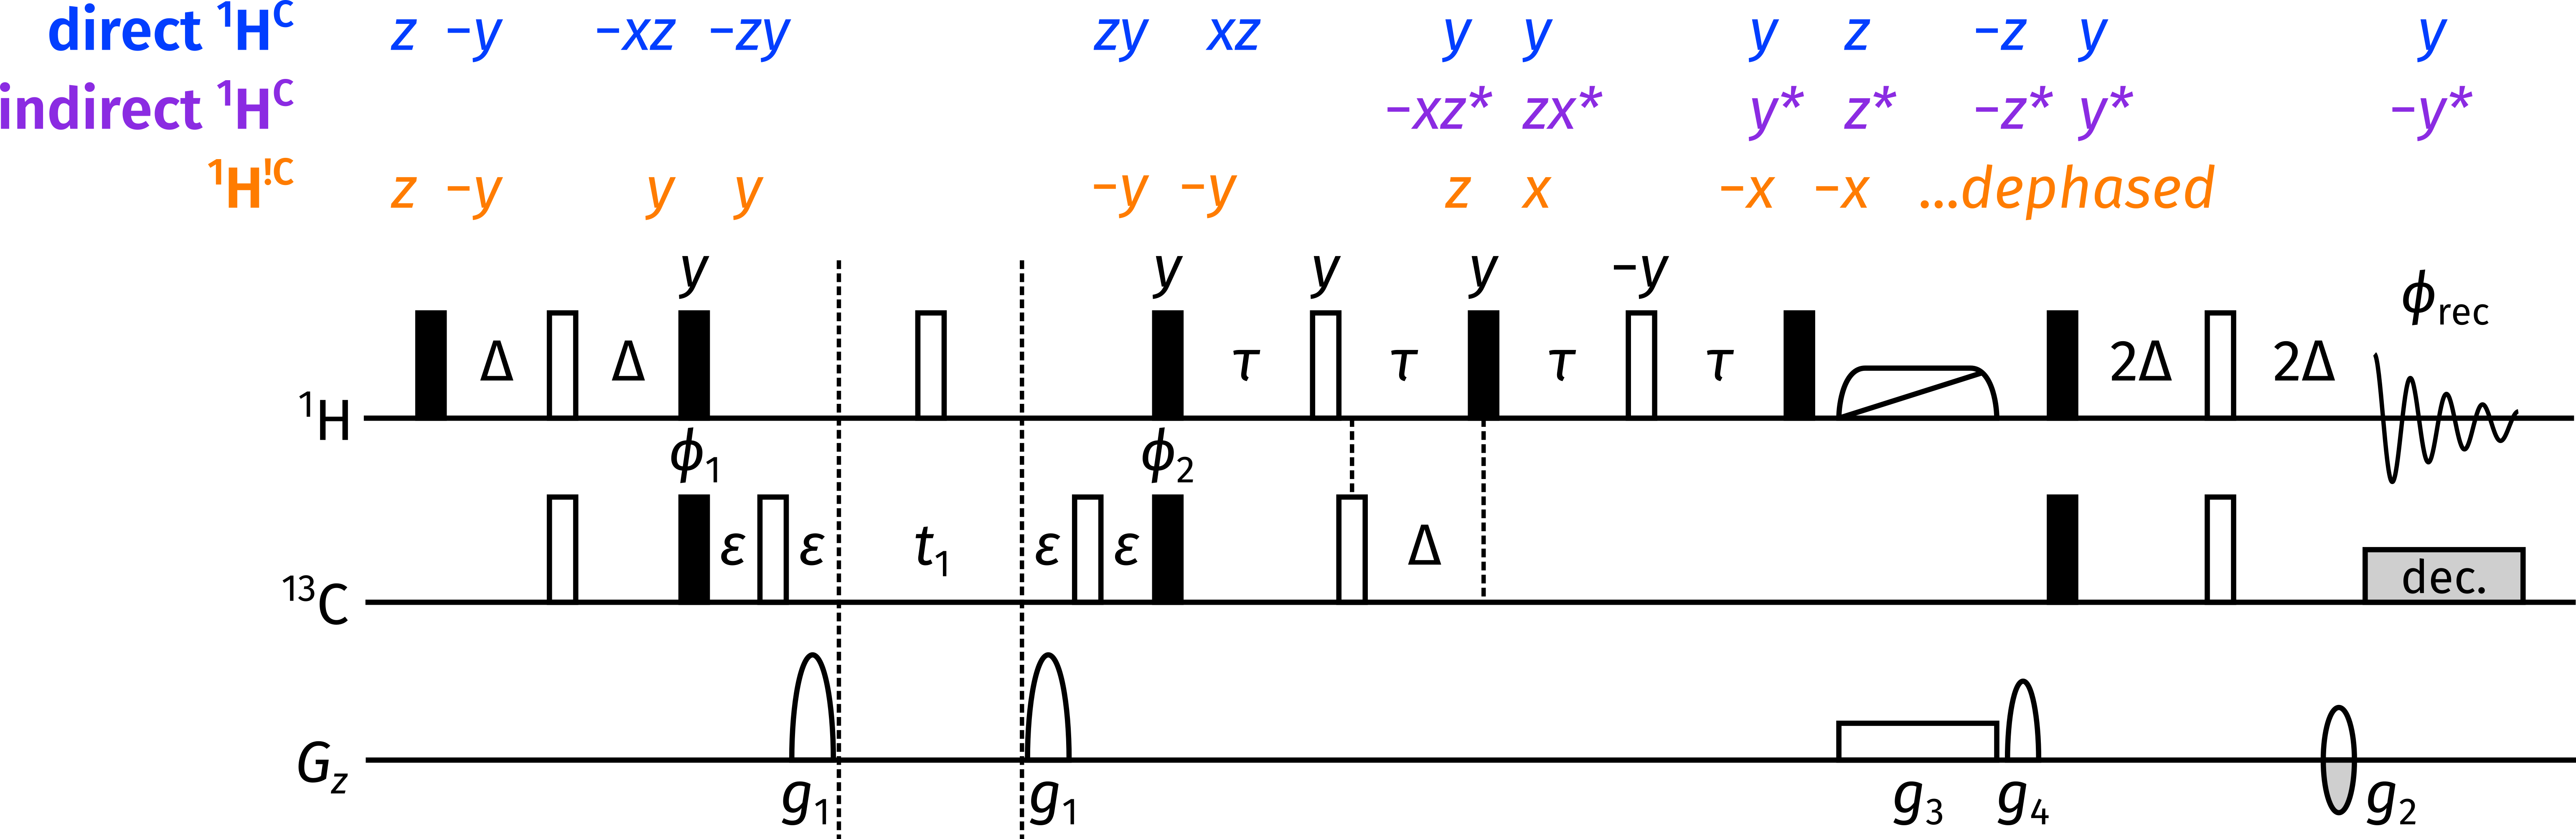
\includegraphics[]{pp/hsqccosy/clip_po.png}%
    \caption[HSQC-CLIP-COSY experiment]{
        HSQC-CLIP-COSY experiment with product operator analysis for the HSQC-COSY signal derived from the \magn{C} magnetisation, as well as the bulk \magnnot{C} magnetisation.
        Both the `direct', HSQC-type peaks, as well as the `indirect' responses arising from coherence transfer in the perfect echo block, are analysed.
        The shorthand notation for product operators is expanded here to deal with a three-spin $IKS$ system, where $I$ and $S$ are a mutually bonded \proton{}--\carbon{} pair as usual, and $K$ is a `remote' proton coupled to $I$.
        Terms with asterisks are on spin $K$; thus, for example, $zx*$ refers to an $I_zK_x$ term.
        The delay $\tau$ is chosen to be $1 / (4 \cdot \sum \nJ{HH})$; typically, this sum of couplings is set as \qty{30}{Hz}, leading to a value of $\tau = \qty{8.33}{\ms}$.
        The ZQF gradient $g_3$ should be calibrated as per Thrippleton et al.\autocite{Thrippleton2003ACIE}; $g_4$ is a purge gradient with arbitrary amplitude.
        All other symbols have the same meaning as in \cref{fig:sehsqc_po}.
    }
    \label{fig:hsqcc_clip_po}
\end{figure}

These problems are circumvented by the HSQC-CLIP-COSY experiment\autocite{Gyongyosi2018CPC,Gyongyosi2021AC}, where the basic HSQC experiment is combined with clean in-phase (CLIP) coherence transfer using a perfect echo\autocite{Aguilar2012CC,Parella2019MRC,Koos2016ACIE} and ZQF\autocite{Thrippleton2003ACIE} (\cref{fig:hsqcc_clip_po}).
The use of an HSQC-type experiment means that $\nJ{HH}$ does not evolve during $t_1$, and the CLIP transfer ensures that all peaks have in-phase absorption lineshapes.
Much like the HSQC-TOCSY experiment before it, this experiment may be implemented with direct/indirect response editing: it is this version of the experiment which is shown in \cref{fig:hsqcc_clip_po}.%
\footnote{Note that this direct/indirect editing is orthogonal to \textit{multiplicity editing}, which labels both direct and indirect responses with a sign that depends on the multiplicity of the \carbon{} nucleus detected in $t_1$. The addition of multiplicity editing leads to highly confusing spectra, so is ignored here---although the option to do so \textit{is} provided in the GENESIS pulse programmes if the user so desires.}
If this editing is not desired, then the final $2\Delta$--\ang{180}($I,S$)--$2\Delta$ spin echo can simply be reduced to a minimal gradient echo, i.e.\ $\varepsilon$--\ang{180}($I$)--$\varepsilon$.

Unfortunately, the HSQC-CLIP-COSY experiment does not preserve \magnnot{C} magnetisation; thus, it cannot be directly used in a NOAH supersequence without sacrificing the sensitivity of terminal homonuclear modules.
In particular, the ZQF used in the HSQC-CLIP-COSY experiment dephases all magnetisation that is not along $z$.
If we wished to retain \magnnot{C} magnetisation, it would therefore have to (somehow) be placed along $z$ during this period, and would have to be differentiated from the HSQC-COSY signal \textit{after} the ZQF, which is not possible.%
\footnote{To be precise, although the $\oneJ{CH}$ Hamiltonian could be used to separate bulk magnetisation and the HSQC-type `direct' responses, the `indirect' responses cannot be differentiated.}
On top of that, the experiment also cannot be modified to provide partial excitation of \magn{C} magnetisation, which limits the ways in which it can be combined with other \carbon{} modules.


\subsubsection{Double spin echo HSQC-COSY}

\begin{figure}[!ht]
    \centering
    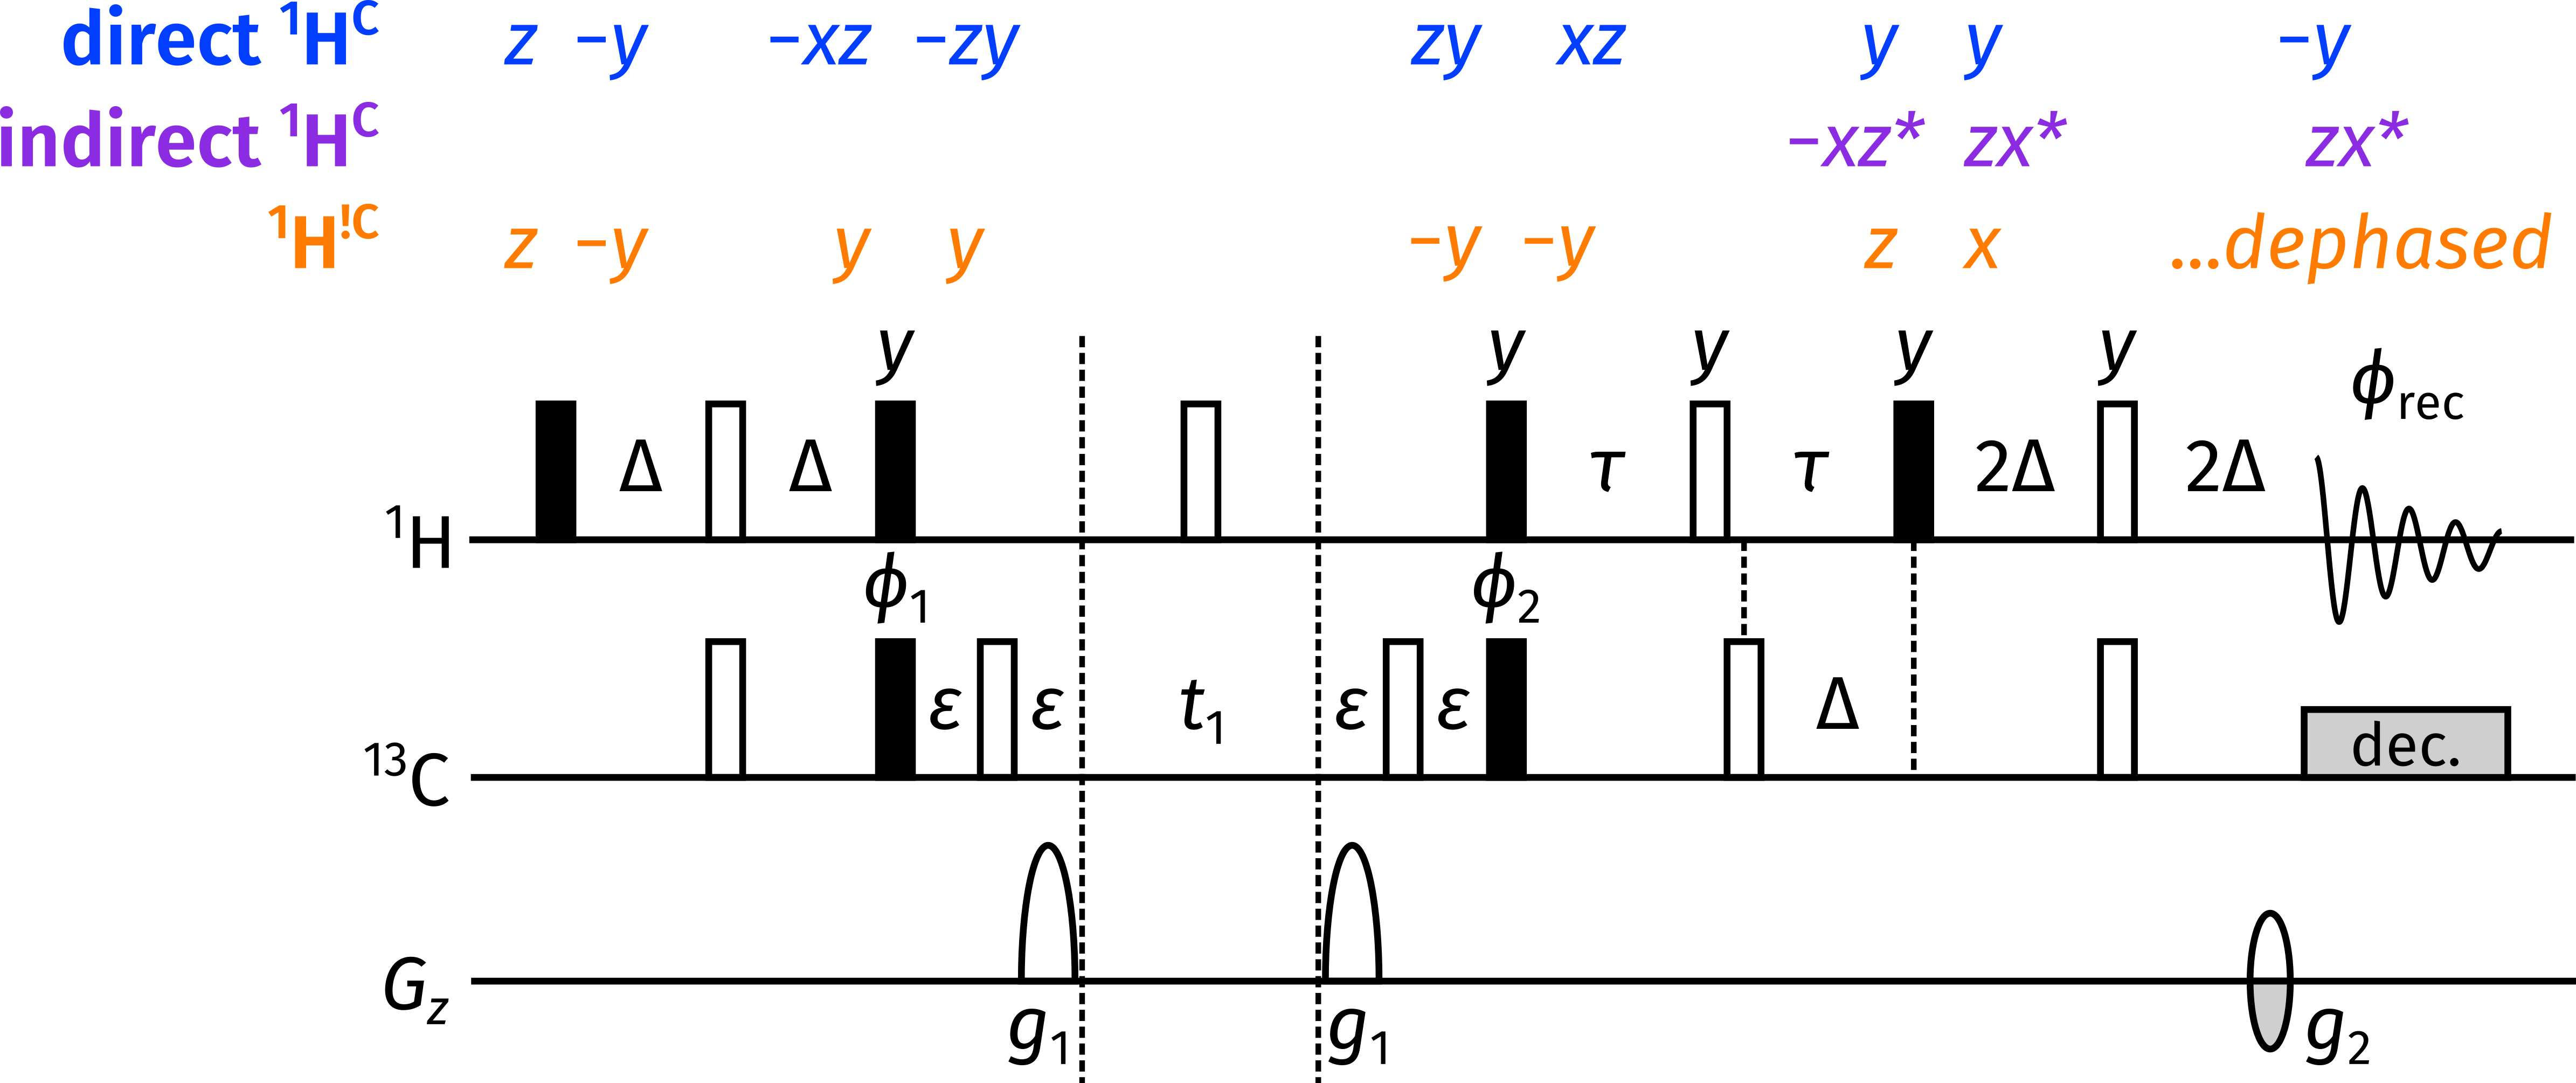
\includegraphics[]{pp/hsqccosy/dse_po.png}%
    \caption[Double spin echo HSQC-COSY experiment]{
        `Double spin echo' HSQC-COSY experiment; all symbols have the same meaning as in \cref{fig:hsqcc_clip_po}.
    }
    \label{fig:hsqcc_dse_po}
\end{figure}

Before tackling these problems directly, I discuss a simpler version of the HSQC-COSY experiment, which uses a simple spin echo for $\nJ{HH}$ evolution instead of the perfect echo of the CLIP version.
Together with the final $4\Delta$ spin echo, this forms a `double spin echo' (DSE) version of the HSQC-COSY experiment (\cref{fig:hsqcc_dse_po}); the `double' refers only to the mixing section after $t_1$.
The removal of the CLIP coherence transfer element leads to mixed lineshapes in this experiment, where the direct responses are (mostly) in-phase absorption, and the indirect responses (mostly) antiphase dispersion.%
\footnote{The qualifier \textit{mostly} is required because evolution of $\nJ{HH}$ during the final spin echo leads to mixtures of in-phase absorption and antiphase dispersion. This evolution is generally small, though, because $2\Delta$ is smaller than $\tau$.}

Like the CLIP version, this DSE experiment does not preserve bulk magnetisation; it is also incompatible with partial \magn{C} excitation.
However, it does provide more raw sensitivity than the CLIP version: in the CLIP version, any antiphase signal at the end of the perfect echo is destroyed by the ZQF.
All of this available signal is sampled in the DSE version, but this comes at the cost of not having pure absorption lineshapes.

It should be mentioned that prepending this DSE HSQC-COSY with the ZIP element would in fact return the bulk \magnnot{C} magnetisation to $+z$ at the end of the sequence.
However, I did not manage to test this experimentally, as my focus was on the development of the \textit{triple} spin echo HSQC-COSY below.


\subsubsection{Triple spin echo HSQC-COSY}

\begin{figure}[!ht]
    \centering
    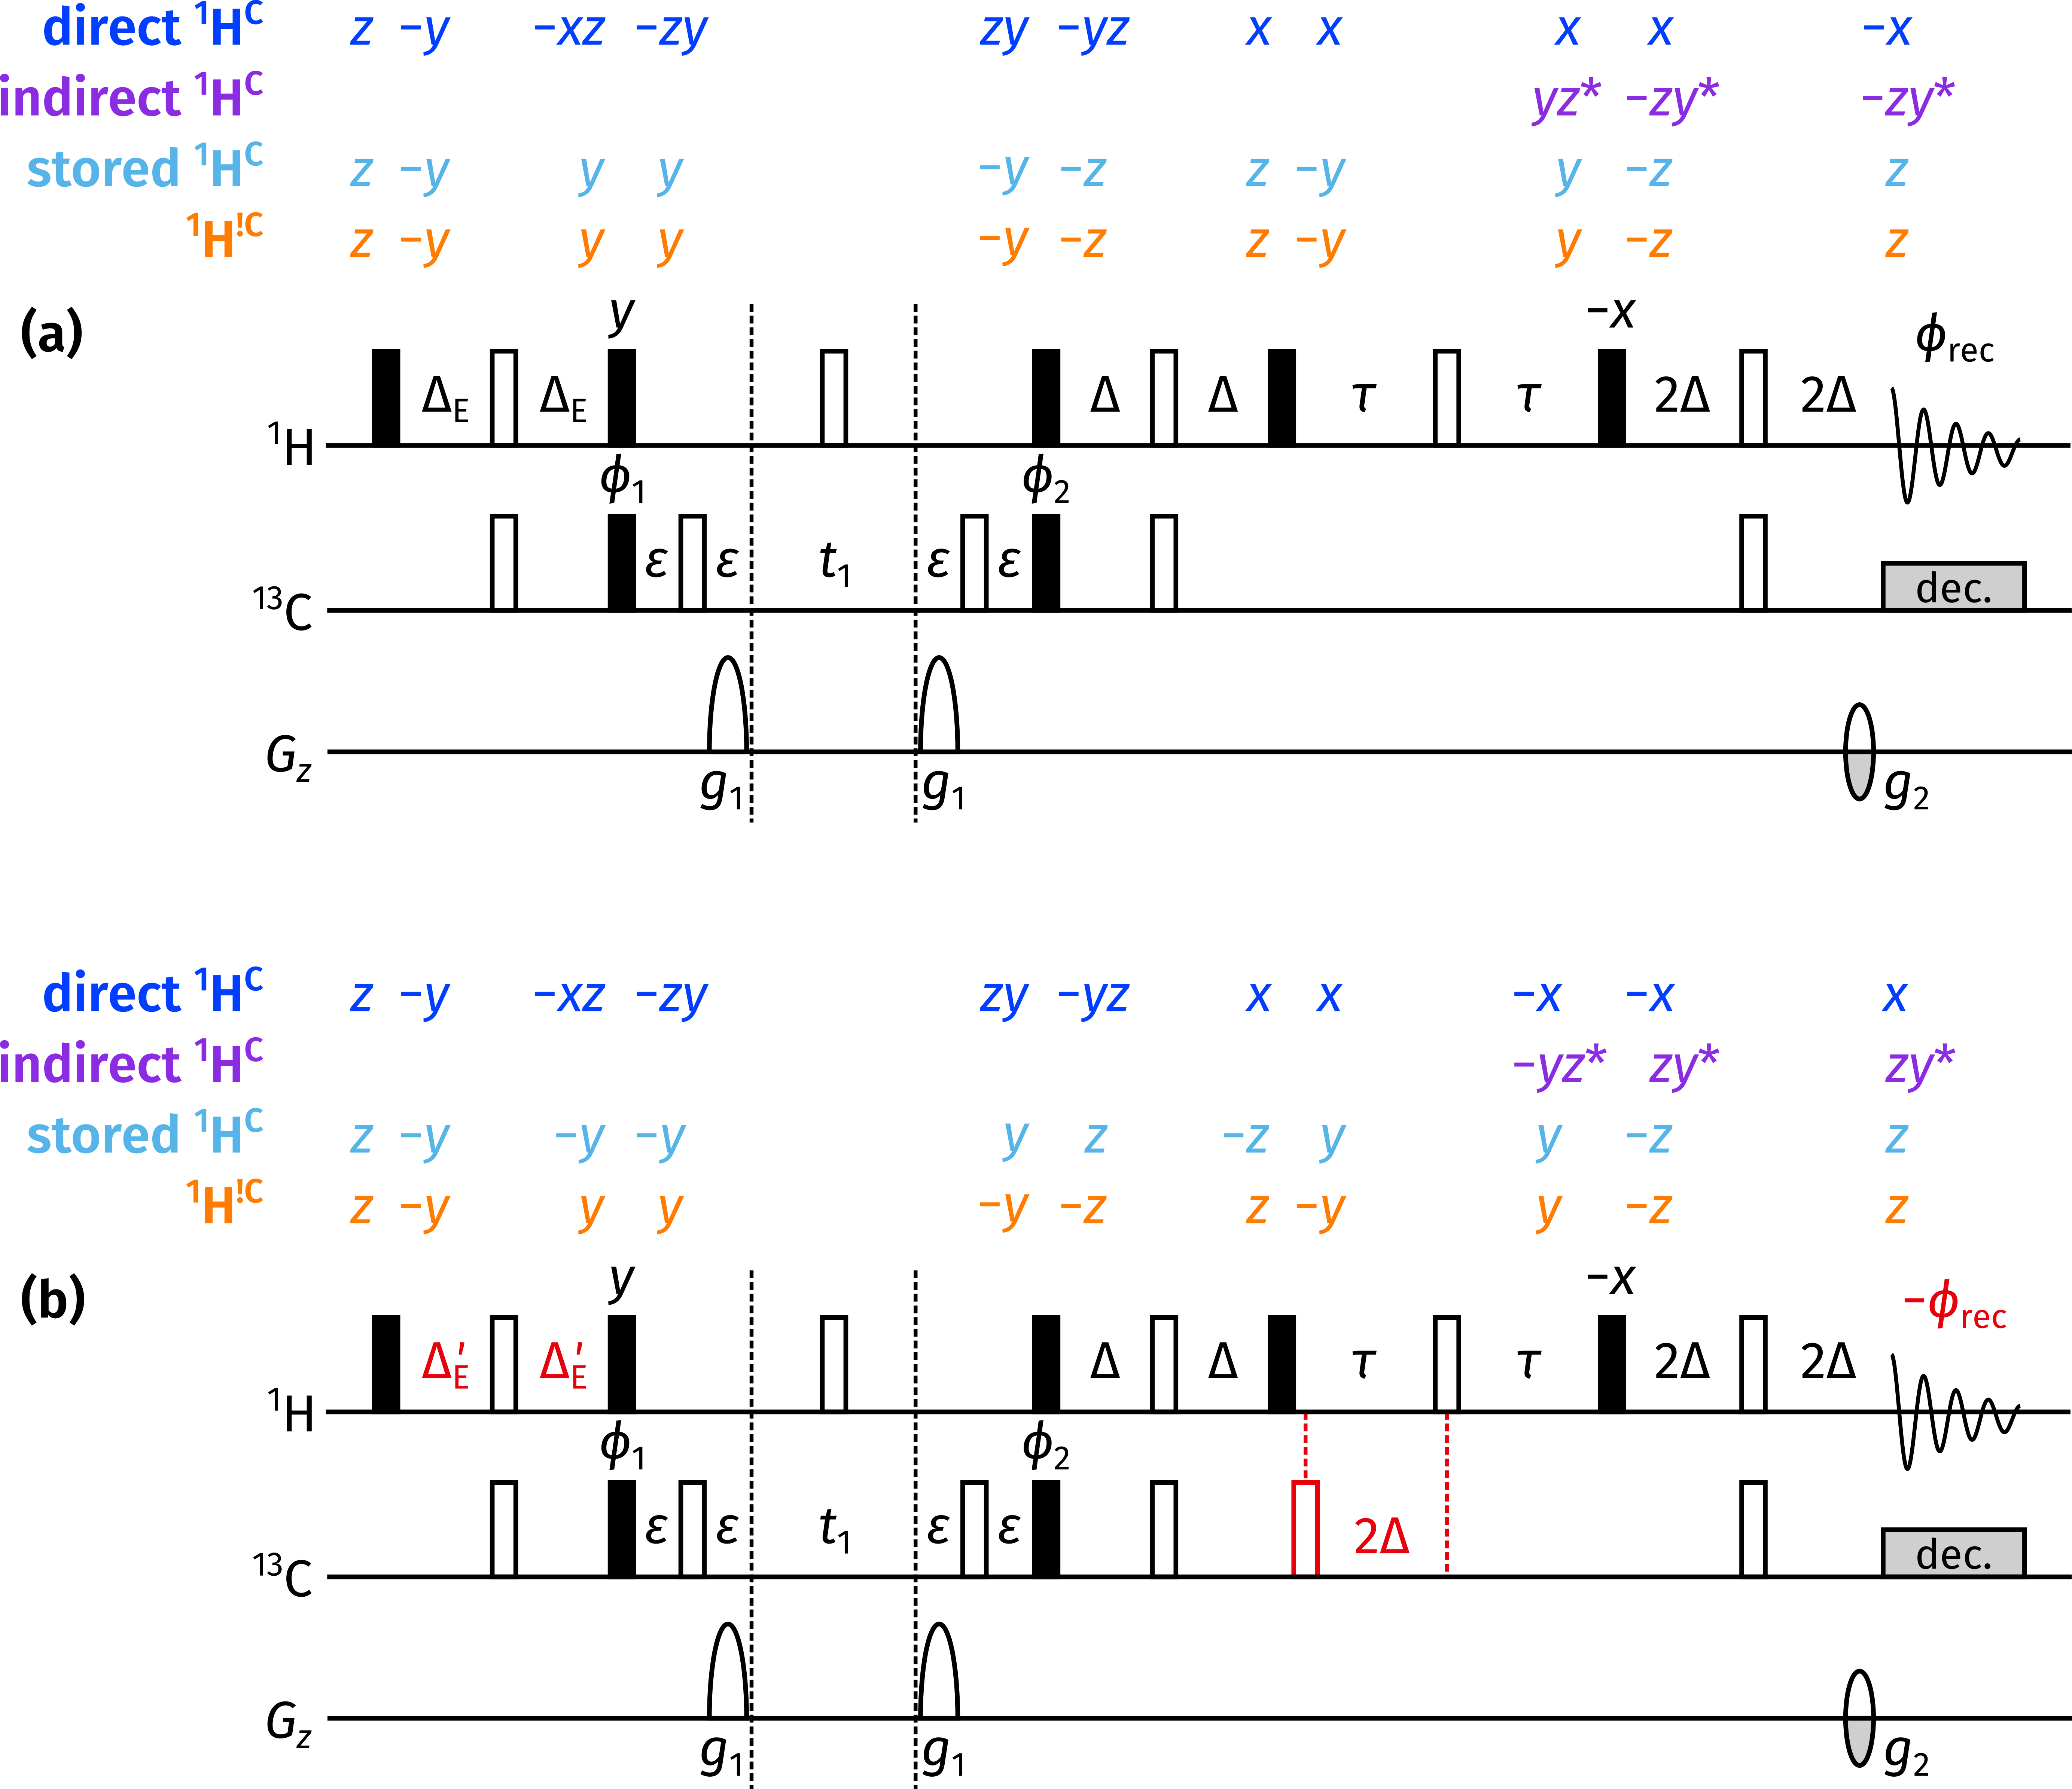
\includegraphics[]{pp/hsqccosy/tse_po.png}%
    {\phantomsubcaption\label{fig:hsqcc_tse_po_1}}%
    {\phantomsubcaption\label{fig:hsqcc_tse_po_2}}%
    \caption[Triple spin echo HSQC-COSY experiment]{
        `Triple spin echo' (TSE) HSQC-COSY experiment.
        \textbf{(\subref*{fig:hsqcc_tse_po_1})} The first part of the experiment; this can be used on its own, but leads to spurious `relayed' peaks arising via coherence transfer over two scalar couplings.
        \textbf{(\subref*{fig:hsqcc_tse_po_2})} The second part of the experiment; co-adding this dataset with the first part leads to suppression of the relayed peaks.
        All symbols have the same meaning as in \cref{fig:hsqcc_clip_po}.
    }
    \label{fig:hsqcc_tse_po}
\end{figure}

In the DSE HSQC-COSY, the first of the two spin echoes after $t_1$ serves a dual purpose: $\oneJ{CH}$ is allowed to evolve for a duration of $\tau - (\tau - \Delta) + \Delta = 2\Delta$ (thus generating peaks which are in-phase with respect to $\oneJ{CH}$), and $\nJ{HH}$ evolves for the total duration of $2\tau$ (allowing coherence transfer to remote spins).
The triple spin echo (TSE) HSQC-COSY is derived from the DSE version by separating the first spin echo into two distinct parts: one for $\oneJ{CH}$ refocusing, and one for $\nJ{HH}$ evolution.
As shown by the product operator analysis in \cref{fig:hsqcc_tse_po_1}, this not only preserves the bulk \magnnot{C} magnetisation, but is also compatible with partial \magn{C} excitation.

The problem with the TSE version is the spectral quality: consider an even larger spin system of the form $\ch{S-I-K-L}$, where $\{I,K,L\}$ are \proton{} and $S\/$ is \carbon{}.
At the end of $t_1$, single-quantum magnetisation on spin $I\/$ is present.
Any evolution of $J_{IK}$ in the first spin echo (of duration $2\Delta$) leads to terms of the form $2I_yK_z$, and can then be transferred onto spin $K\/$ by the subsequent \angang{90}{x} pulse.
This magnetisation can then further evolve under $J_{KL}$ during the $2\tau$ spin echo, and then be transferred a \textit{second} time by the \angang{90}{-x} pulse to spin $L$.
Since the intensity of this transfer pathway is proportional to $\sin(2\cpi J_{IK}\Delta)$, these `relay' artefacts are especially prominent for large $J_{IK}$.

In order to suppress these, the experiment must be run a second time but with an additional \ang{180} \carbon{} pulse inserted during the second spin echo (\cref{fig:hsqcc_tse_po_2}).%
\footnote{A very similar strategy is used in the Bruker seHSQC pulse sequence \texttt{hsqcedetgpsisp2.4} to suppress the COSY-type artefacts. However, to the best of my knowledge, this sequence has not been published anywhere.}
Any magnetisation still on spin $I\/$ will therefore evolve under $\oneJ{CH}$ for a total period of $4\Delta$, leading to net inversion.
However, magnetisation which has already been transferred to spin $K\/$ at this point will not be inverted: it is this magnetisation which is responsible for the relay artefacts.
Therefore, by subtracting the two datasets (or equivalently, inverting the receiver phase and adding the two datasets), the desired peaks will be added up and the artefacts cancelled through subtraction.

The insertion of this \ang{180} pulse also causes any unexcited \magn{C} magnetisation to be inverted.
In order to ensure that this is returned to $+z$ at the end of the sequence (and not $-z$), the initial INEPT delay must be \textit{lengthened} instead of shortened, as per:
\begin{equation}
    \label{eq:delta_e_prime}
    \DeltaE' = \frac{2\Delta (\cpi - \arcsin f)}{\cpi},
\end{equation}
where, as before, $f\/$ is the proportion of magnetisation to be excited.


\subsubsection{Supersequences}

\begin{figure}[!htp]
    \centering
    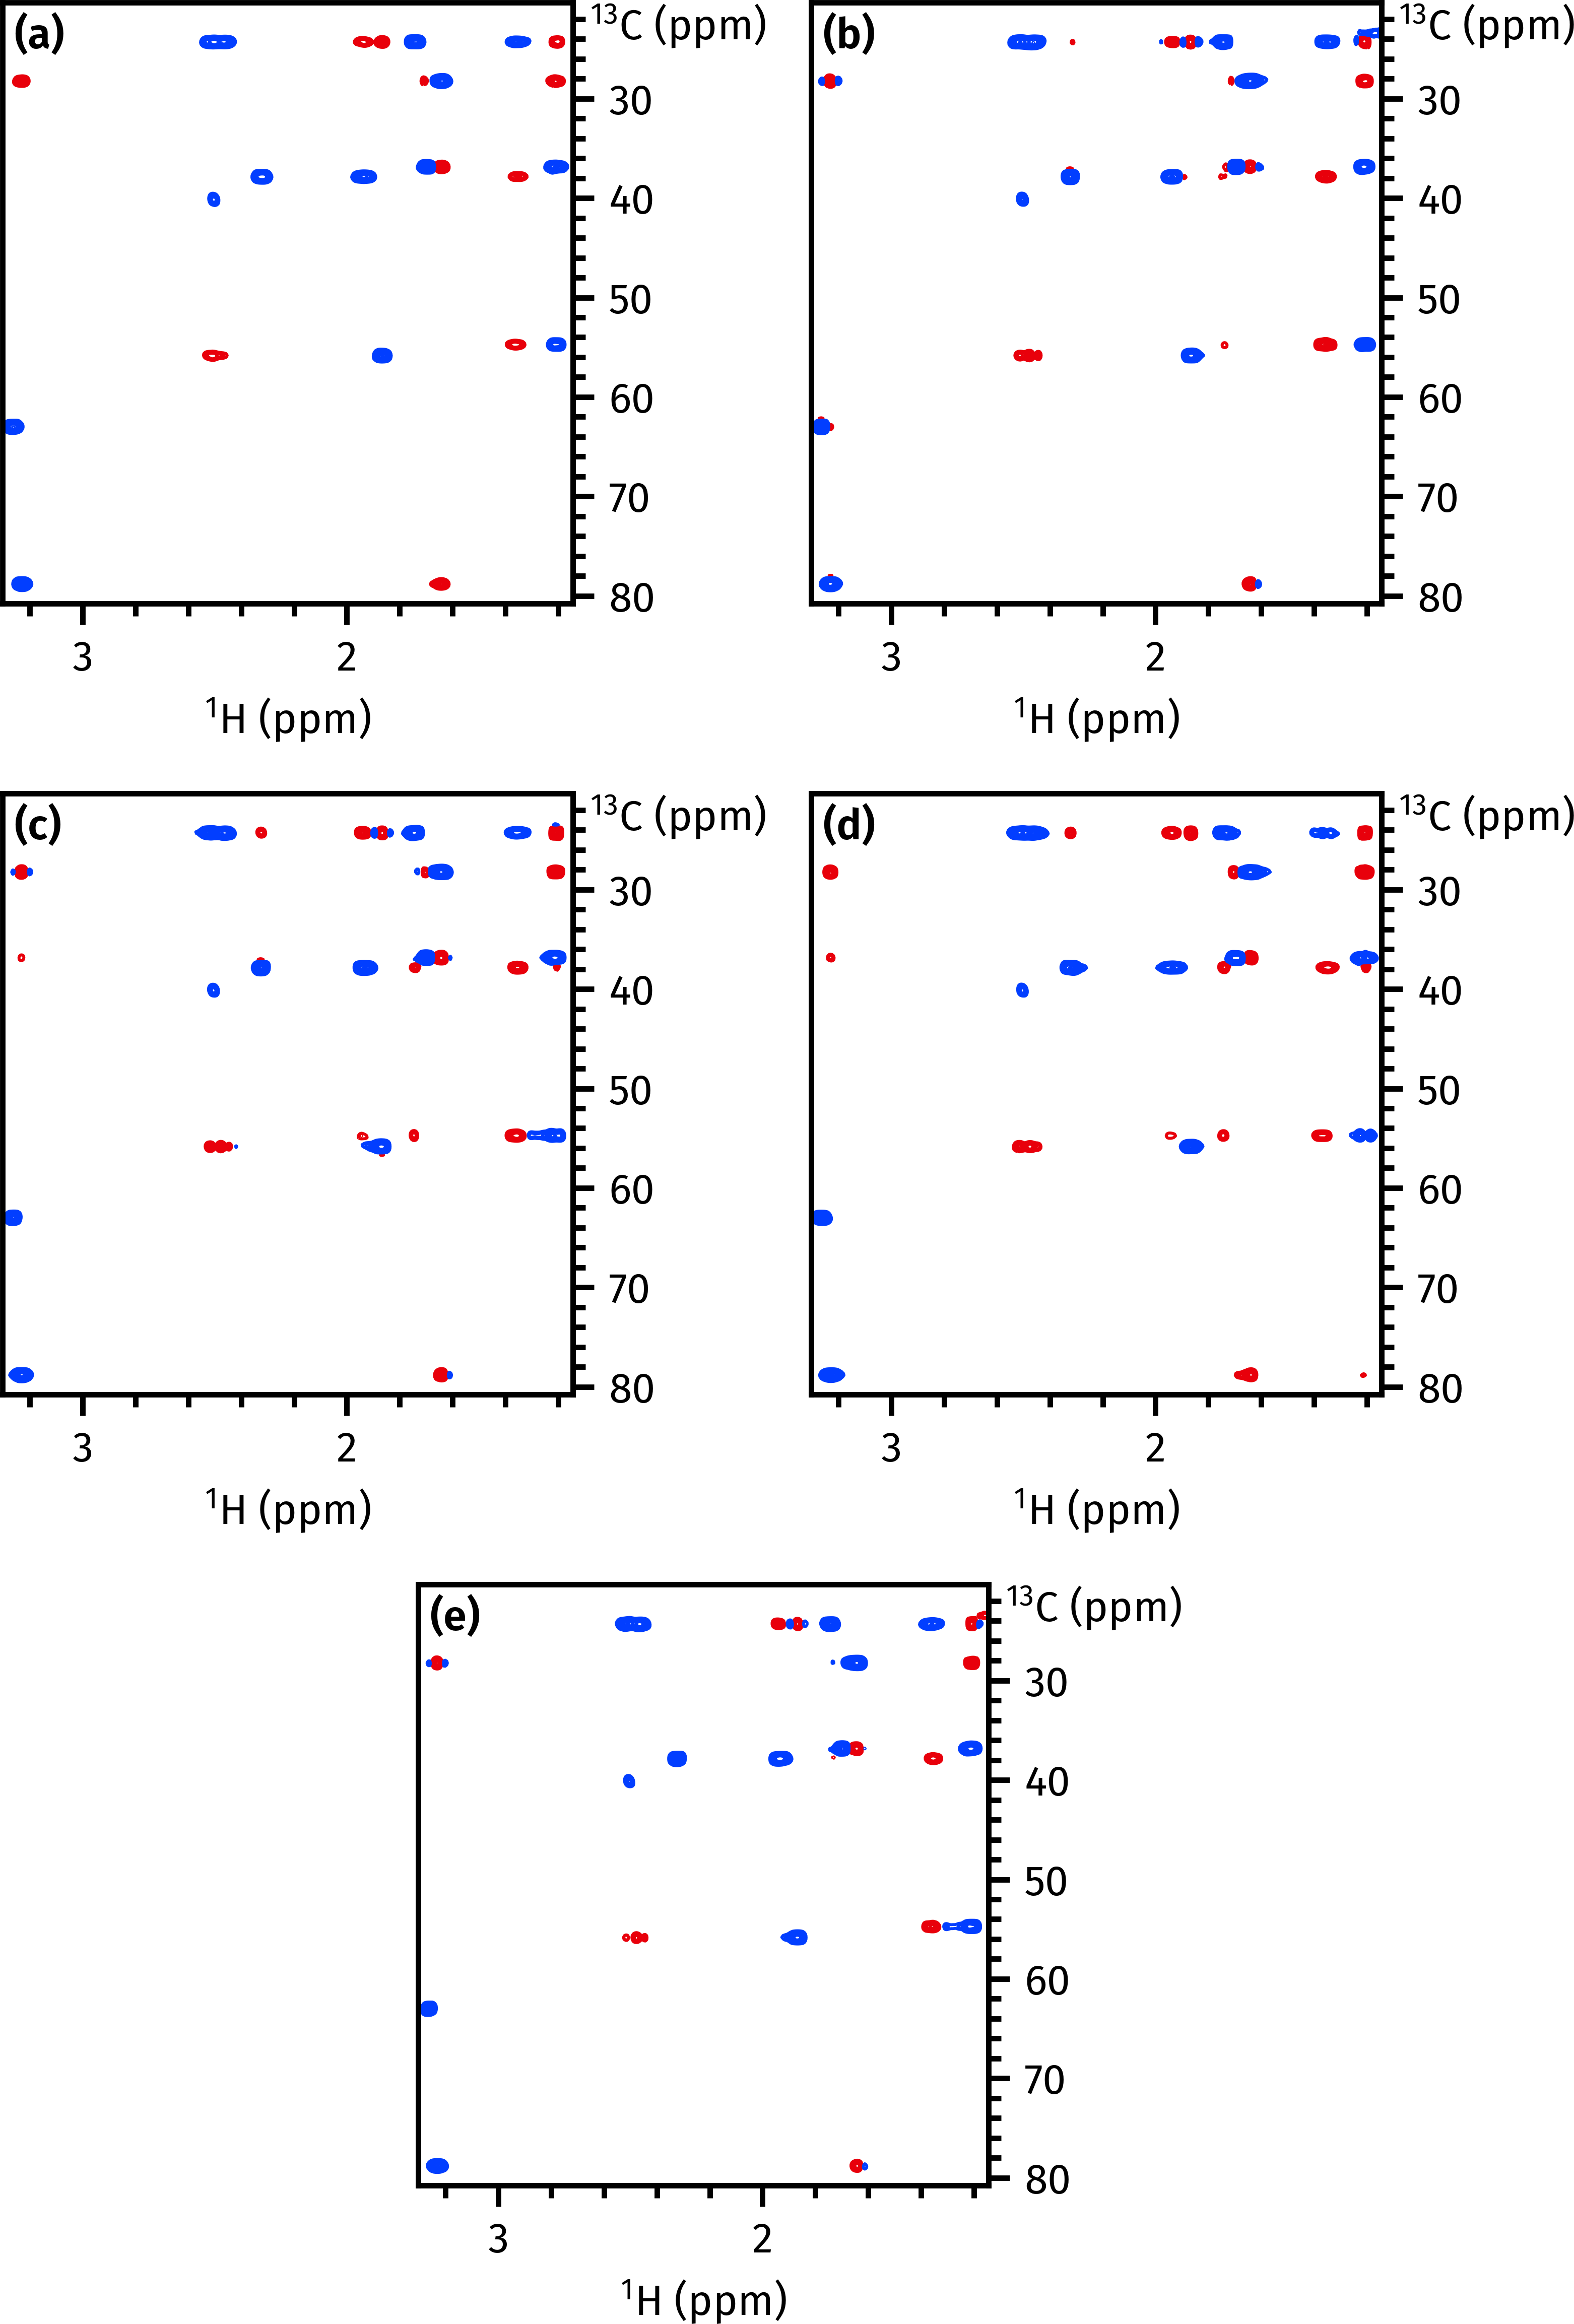
\includegraphics[]{noah/hsqccosy_comp.png}%
    {\phantomsubcaption\label{fig:hsqccosy_comp_clip}}%
    {\phantomsubcaption\label{fig:hsqccosy_comp_dse}}%
    {\phantomsubcaption\label{fig:hsqccosy_comp_tse_norps}}%
    {\phantomsubcaption\label{fig:hsqccosy_comp_tocsy}}%
    {\phantomsubcaption\label{fig:hsqccosy_comp_tse}}%
    \caption[Comparison of spectra acquired with different HSQC-COSY modules]{
        HSQC-COSY and HSQC-TOCSY spectra, taken from (respectively) \noah{Sc,S,Cc} and \noah{St,S,Cc} experiments.
        \textbf{(\subref*{fig:hsqccosy_comp_clip})} HSQC-CLIP-COSY.
        \textbf{(\subref*{fig:hsqccosy_comp_dse})} DSE HSQC-COSY.
        \textbf{(\subref*{fig:hsqccosy_comp_tse_norps})} TSE HSQC-COSY without suppression of relay artefacts (described in the text).
        \textbf{(\subref*{fig:hsqccosy_comp_tocsy})} HSQC-TOCSY with \qty{10}{\ms} mixing time.
        \textbf{(\subref*{fig:hsqccosy_comp_tse})} TSE HSQC-COSY with suppression of relay artefacts.
        \datacode{7A-210303}
    }
    \label{fig:hsqccosy_comp}
\end{figure}

\begin{figure}[!ht]
    \centering
    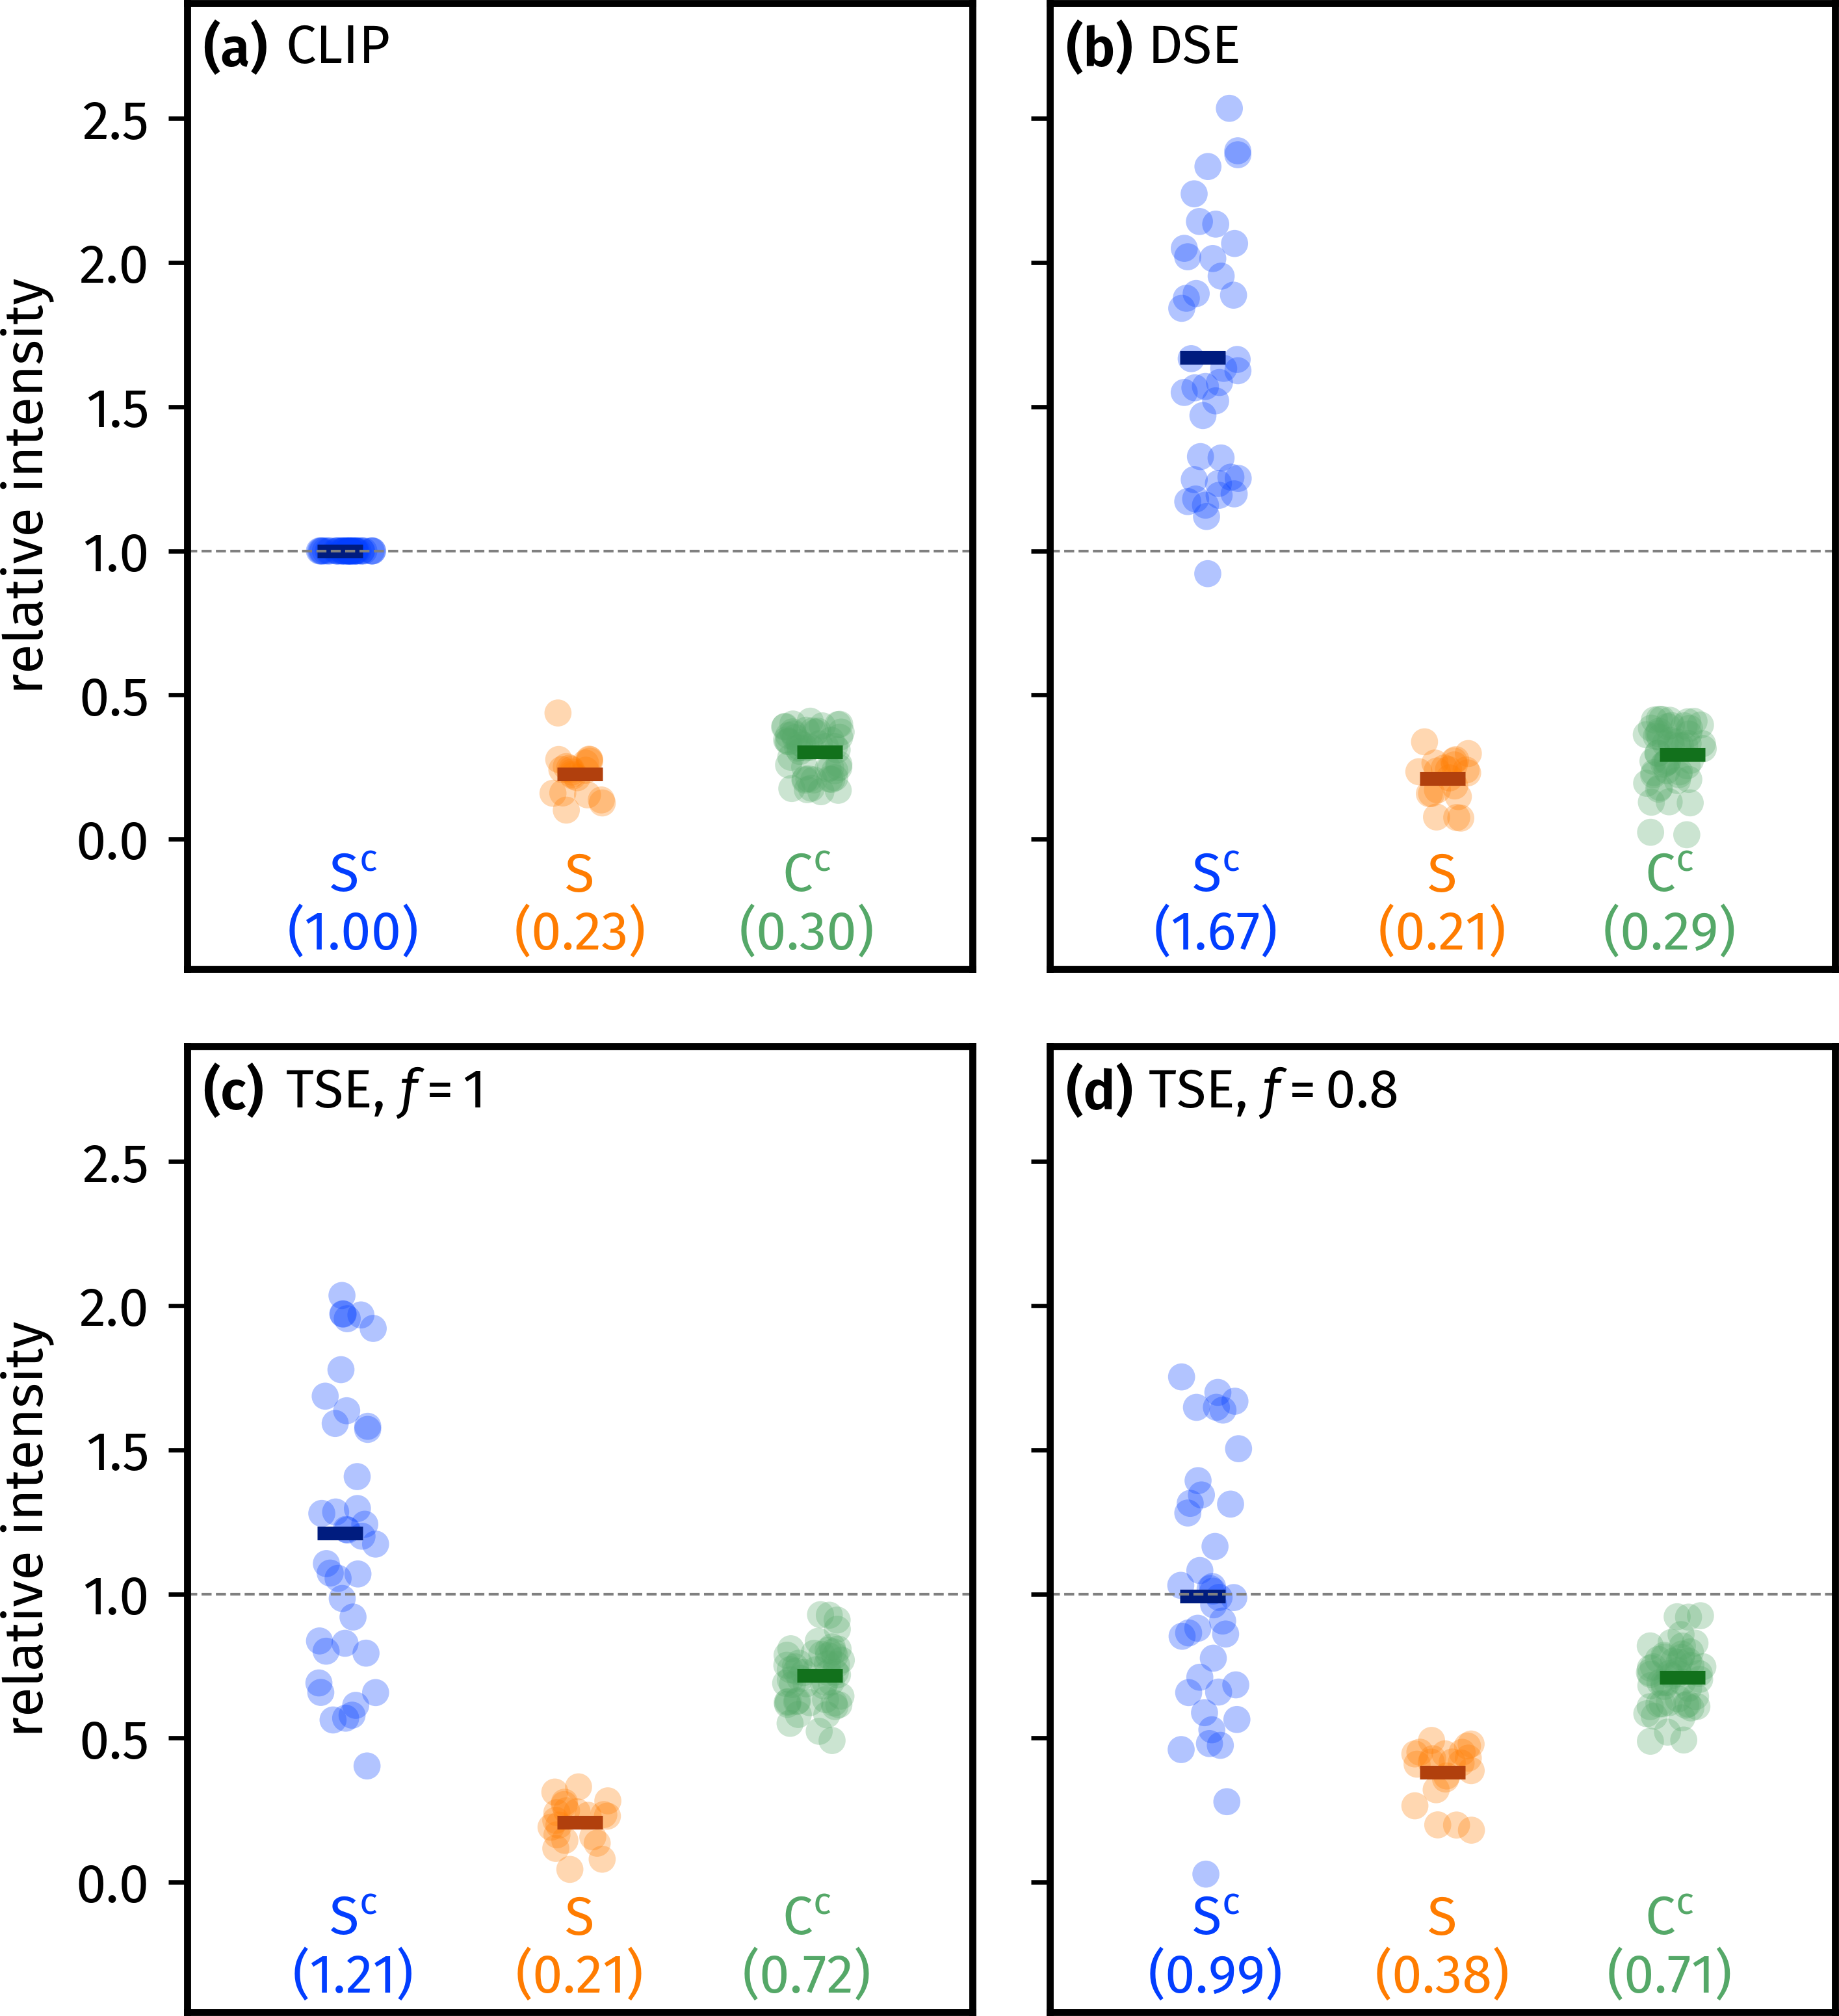
\includegraphics[]{noah/hsqccosy_sens.png}%
    {\phantomsubcaption\label{fig:hsqccosy_sens_clip}}%
    {\phantomsubcaption\label{fig:hsqccosy_sens_dse}}%
    {\phantomsubcaption\label{fig:hsqccosy_sens_tse_1}}%
    {\phantomsubcaption\label{fig:hsqccosy_sens_tse_0p8}}%
    \caption[Sensitivity comparisons for \noah{Sc,S,Cc} supersequences]{
        Sensitivity comparisons for all three modules in \noah{Sc,S,Cc} supersequences.
        Peak intensities are relative to the HSQC-CLIP-COSY module itself (the leftmost column in (\subref*{fig:hsqccosy_sens_clip})), as well as HSQC and CLIP-COSY spectra from a \noah{S,Cc} experiment.
        Numbers in parentheses indicate averages over all peaks.
        \textbf{(\subref*{fig:hsqccosy_sens_clip})} HSQC-CLIP-COSY.
        \textbf{(\subref*{fig:hsqccosy_sens_dse})} DSE HSQC-COSY.
        \textbf{(\subref*{fig:hsqccosy_sens_tse_1})} TSE HSQC-COSY, acquired with $f = 1$.
        \textbf{(\subref*{fig:hsqccosy_sens_tse_0p8})} TSE HSQC-COSY, acquired with $f = 0.8$.
        \datacode{7A-210723}
    }
    \label{fig:hsqccosy_sens}
\end{figure}

The spectral quality, and sensitivity, of all of these modules is captured in \cref{fig:hsqccosy_comp,fig:hsqccosy_sens}.
The CLIP version (\cref{fig:hsqccosy_comp_clip,fig:hsqccosy_sens_clip}) has the best lineshapes, but its sensitivity is slightly lower.
The DSE version (\cref{fig:hsqccosy_comp_dse,fig:hsqccosy_sens_dse}) provides greater sensitivity, but at the cost of impure lineshapes.

For the TSE version, we first look at the importance of the relay artefact suppression procedure described above.
The extra relay artefacts are clearly visible in \cref{fig:hsqccosy_comp_tse_norps}, acquired using the `basic' sequence in \cref{fig:hsqcc_tse_po_1} only.
(As previously mentioned, these arise from large $\nJ{HH}$ which evolve during the $2\Delta$ spin echo; for this specific compound, the offending couplings are $^3\!J\/$ between two axial protons in a six-membered ring, and $^2\!J\/$ in diastereotopic methylenes).
The presence of these peaks largely defeats the purpose of using an HSQC-COSY experiment; in fact, this unoptimised TSE HSQC-COSY is qualitatively very similar to an HSQC-TOCSY acquired with a short mixing time of \qty{10}{\ms} (\cref{fig:hsqccosy_comp_tocsy}).%
\footnote{The HSQC-TOCSY even gives better peak shapes, since the DIPSI mixing transfers in-phase magnetisation to in-phase magnetisation.}
However, these artefacts can be efficiently removed using the suppression technique described in the text above; the result in \cref{fig:hsqccosy_comp_tse} is qualitatively similar to the two other HSQC-COSY experiments.
Using this suppression technique, the sensitivity of the TSE HSQC-COSY (when acquired with $f = 1$) falls between that of the CLIP and DSE versions.

\Cref{fig:hsqccosy_sens} also shows the relative sensitivities of the later modules in \noah{Sc,S,Cc} supersequences.
In all of the first three cases (CLIP, DSE, and TSE HSQC-COSY with $f = 1$, \cref{fig:hsqccosy_sens_clip,fig:hsqccosy_sens_dse,fig:hsqccosy_sens_tse_1}), the HSQC sensitivity is low (ca.\ 20\%) because no \magn{C} magnetisation is retained for it to use.
Thus, the signal derives only from \magn{C} magnetisation which has recovered during the HSQC-COSY FID.
However, when the TSE version is used, partial \magn{C} excitation can be used to control this sensitivity: for example, when $f = 0.8$ (\cref{fig:hsqccosy_sens_tse_0p8}), the HSQC-COSY sensitivity is decreased (on average equalling that of the HSQC-CLIP-COSY), but the sensitivity of the HSQC module is almost doubled.
Generally, choosing a value of $f < 1$ allows for the HSQC-COSY and HSQC sensitivities to be better balanced.

Finally, the CLIP-COSY module suffers when the HSQC-CLIP-COSY or the DSE HSQC-COSY are used, because both of these dephase \magnnot{C} magnetisation;
however, the TSE version successfully preserves around $70\%$ of this magnetisation for it, regardless of the value of $f$.
(This value is slightly lower than the approximately $90\%$ magnetisation preserved by the HSQC module, because the bulk magnetisation is placed in the transverse plane during the $2\tau$ spin echo (\cref{fig:hsqcc_tse_po_1}) and experiences losses due to $\nJ{HH}$ evolution.)


\subsubsection{HSQC-COSY in context}

\begin{figure}[!ht]
    \centering
    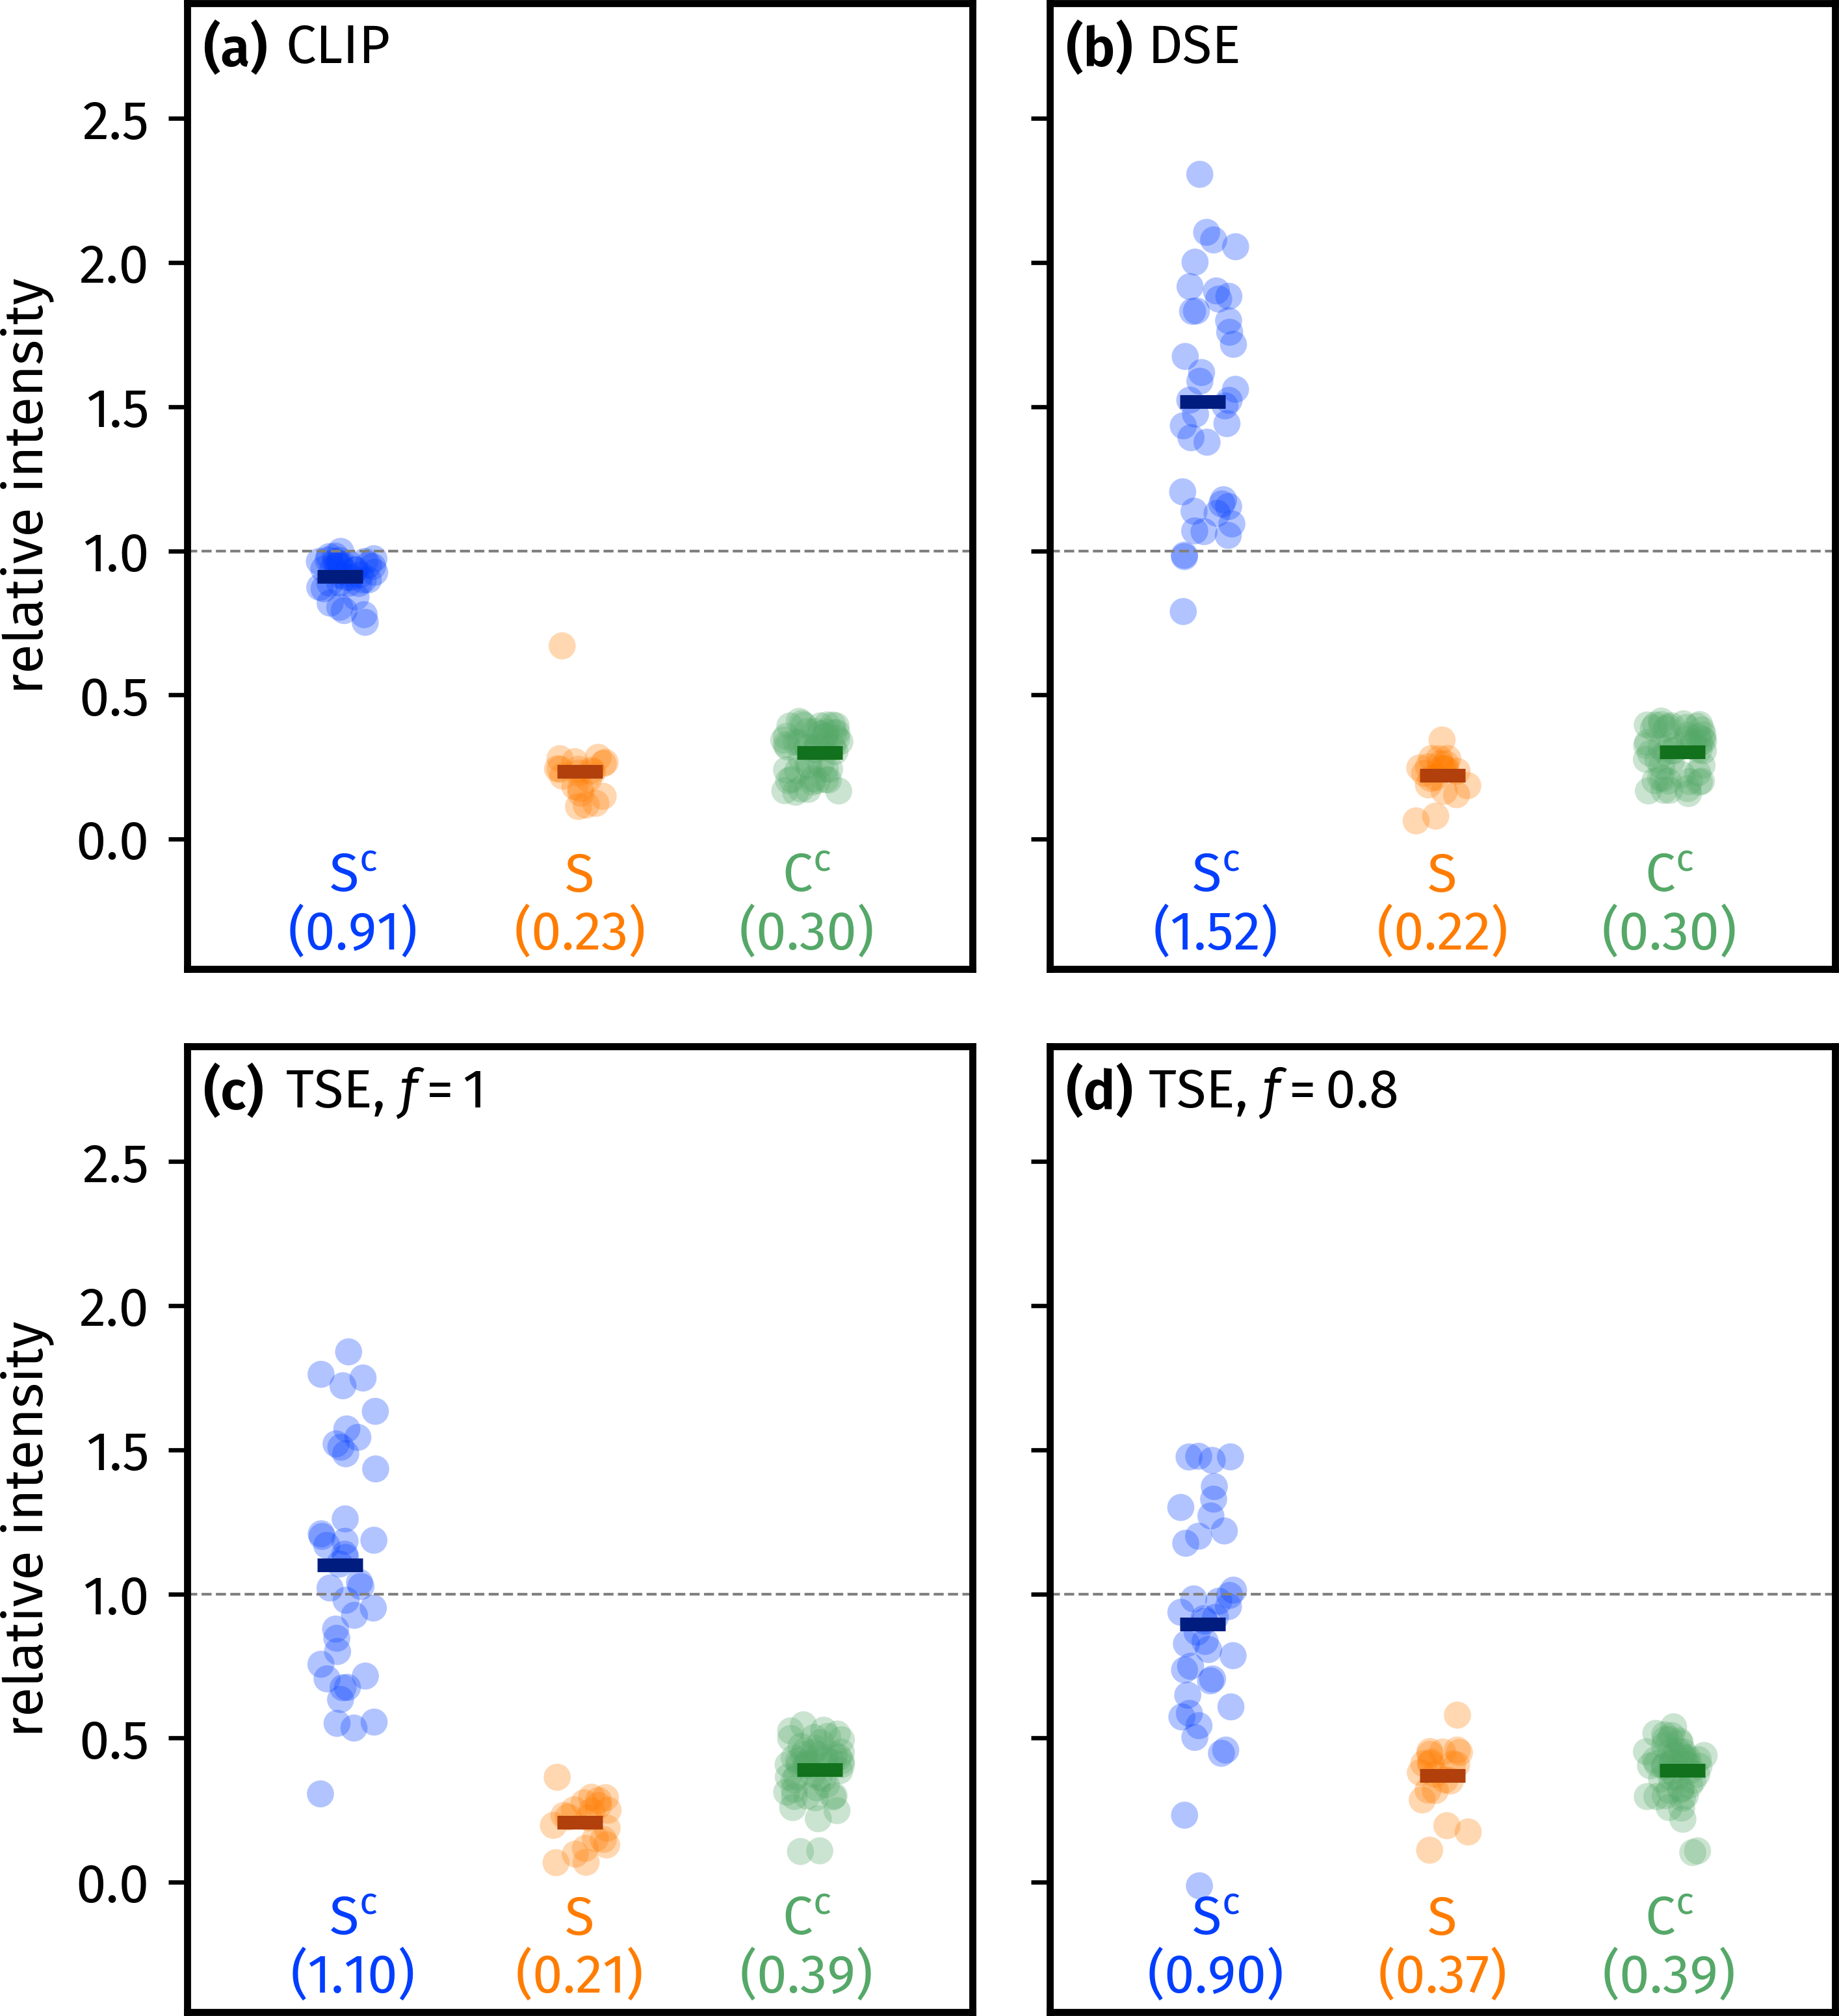
\includegraphics[]{noah/hsqccosy_sens_with_hmbc.png}%
    {\phantomsubcaption\label{fig:hsqccosy_sens_with_hmbc_clip}}%
    {\phantomsubcaption\label{fig:hsqccosy_sens_with_hmbc_dse}}%
    {\phantomsubcaption\label{fig:hsqccosy_sens_with_hmbc_tse_1}}%
    {\phantomsubcaption\label{fig:hsqccosy_sens_with_hmbc_tse_0p8}}%
    \caption[Sensitivity comparisons for \noah{B,Sc,S,Cc} supersequences]{
        Sensitivity comparisons for the three last modules in \noah{B,Sc,S,Cc} supersequences.
        Peak intensities are relative to the HSQC-CLIP-COSY module from a \noah{Sc,S,Cc} supersequence, and HSQC and CLIP-COSY spectra from a \noah{S,Cc} experiment (these are the same reference spectra as used in \cref{fig:hsqccosy_sens}).
        Numbers in parentheses indicate averages over all peaks.
        \textbf{(\subref*{fig:hsqccosy_sens_with_hmbc_clip})} HSQC-CLIP-COSY.
        \textbf{(\subref*{fig:hsqccosy_sens_with_hmbc_dse})} DSE HSQC-COSY.
        \textbf{(\subref*{fig:hsqccosy_sens_with_hmbc_tse_1})} TSE HSQC-COSY, acquired with $f = 1$.
        \textbf{(\subref*{fig:hsqccosy_sens_with_hmbc_tse_0p8})} TSE HSQC-COSY, acquired with $f = 0.8$.
        \datacode{7A-210723}
    }
    \label{fig:hsqccosy_sens_with_hmbc}
\end{figure}

In \noah{Sc,S,Cc}-type supersequences, using the TSE HSQC-COSY module here appears to be a sensible option as it is capable of preserving some \magn{C} magnetisation for the HSQC, as well as all \magnnot{C} magnetisation for the CLIP-COSY.
However, this may not necessarily be so important in the context of a larger supersequence---particularly one which begins with the HMBC module, which \textit{already} dephases \magnnot{C} magnetisation (meaning that there is not much of it to preserve).

\Cref{fig:hsqccosy_sens_with_hmbc} provides the same sensitivity comparisons as in \cref{fig:hsqccosy_sens}, but in the context of a \noah{B,Sc,S,Cc} supersequence instead.
The HSQC-COSY and HSQC modules largely follow the same pattern as before, but with an approximate 10\% loss across the board: this reflects the imperfect preservation of \magn{C} magnetisation by the $zz$-HMBC module.
The CLIP-COSY module, however, has a substantially lower sensitivity regardless of which HSQC-COSY module is chosen.
When the CLIP or DSE HSQC-COSY modules are used, the CLIP-COSY retains only roughly 30\% of its original intensity: this is the same as in \cref{fig:hsqccosy_sens}.
With the TSE HSQC-COSY, this is boosted to around 40\% because there is one extra FID in which the \magnnot{C} polarisation can be recovered.
However, the use of the HMBC module at the beginning effectively places an upper limit on the amount of signal available to this module.

For virtually all homonuclear modules (including the CLIP-COSY), this small difference in sensitivity will not make a real difference in the interpretability of the spectrum.
This is especially so considering that the HMBC module---which has a far lower sensitivity---is also present in the supersequence:
a CLIP-COSY with 30\% of its original sensitivity is still more intense than the HMBC experiment.
This argument was used in justifying the \noah{B,S,Cc} experiment, and logically, should be equally applicable to the \noah{B,Sc,S,Cc} experiment.
In this case, the only compelling reason to use the TSE HSQC-COSY would be to preserve a portion of \magn{C} magnetisation for a later \carbon{} module.
Thus, in this context, the decision of which HSQC-COSY module to use is slightly more nuanced: the cleaner lineshapes provided by the CLIP version, or the sensitivity of the DSE version, may be more preferable.

\subsection{2DJ and PSYCHE}
\label{subsec:noah__2djpsyche}

`Normal' homonuclear modules are almost trivial to include in NOAH supersequences: since these are placed at the end of supersequences, there is rarely any need to modify them, as they do not need to preserve any magnetisation.
One exception to this is the family of 2DJ and pseudo-2D pure shift experiments (here typified by PSYCHE), where the spectral width in the indirect dimension is extremely small, on the order of \qty{50}{\Hz}.
In such cases, the number of $t_1$ increments required is far smaller than for a typical 2D experiment.
Since---by default---each module in a NOAH supersequence is acquired with the same number of increments, directly adding such modules to the end of a supersequence would therefore prove suboptimal.

However, as described previously in \cref{subsec:noah__sehsqc_n}, it is possible to reduce the number of $t_1$ increments for a particular module, and in exchange, increase the number of scans recorded for that module.
In the context of \nitrogen{} modules, this was a `special' procedure referred to as $k$-scaling; however, for these homonuclear modules, it is natural and necessary.
One difference in the implementation is that, instead of specifying a value $k$ by which \texttt{TD1} is scaled down by and \texttt{NS} scaled up by, the user is allowed to directly specify the number of $t_1$ increments as an integer (\texttt{CNST37} in TopSpin).
This value must be a divisor of \texttt{TD1/NBL}, i.e., the number of $t_1$ increments for all other modules.
The indirect-dimension spectral width is specified as \texttt{CNST38}.

\begin{figure}[!ht]
    \centering
    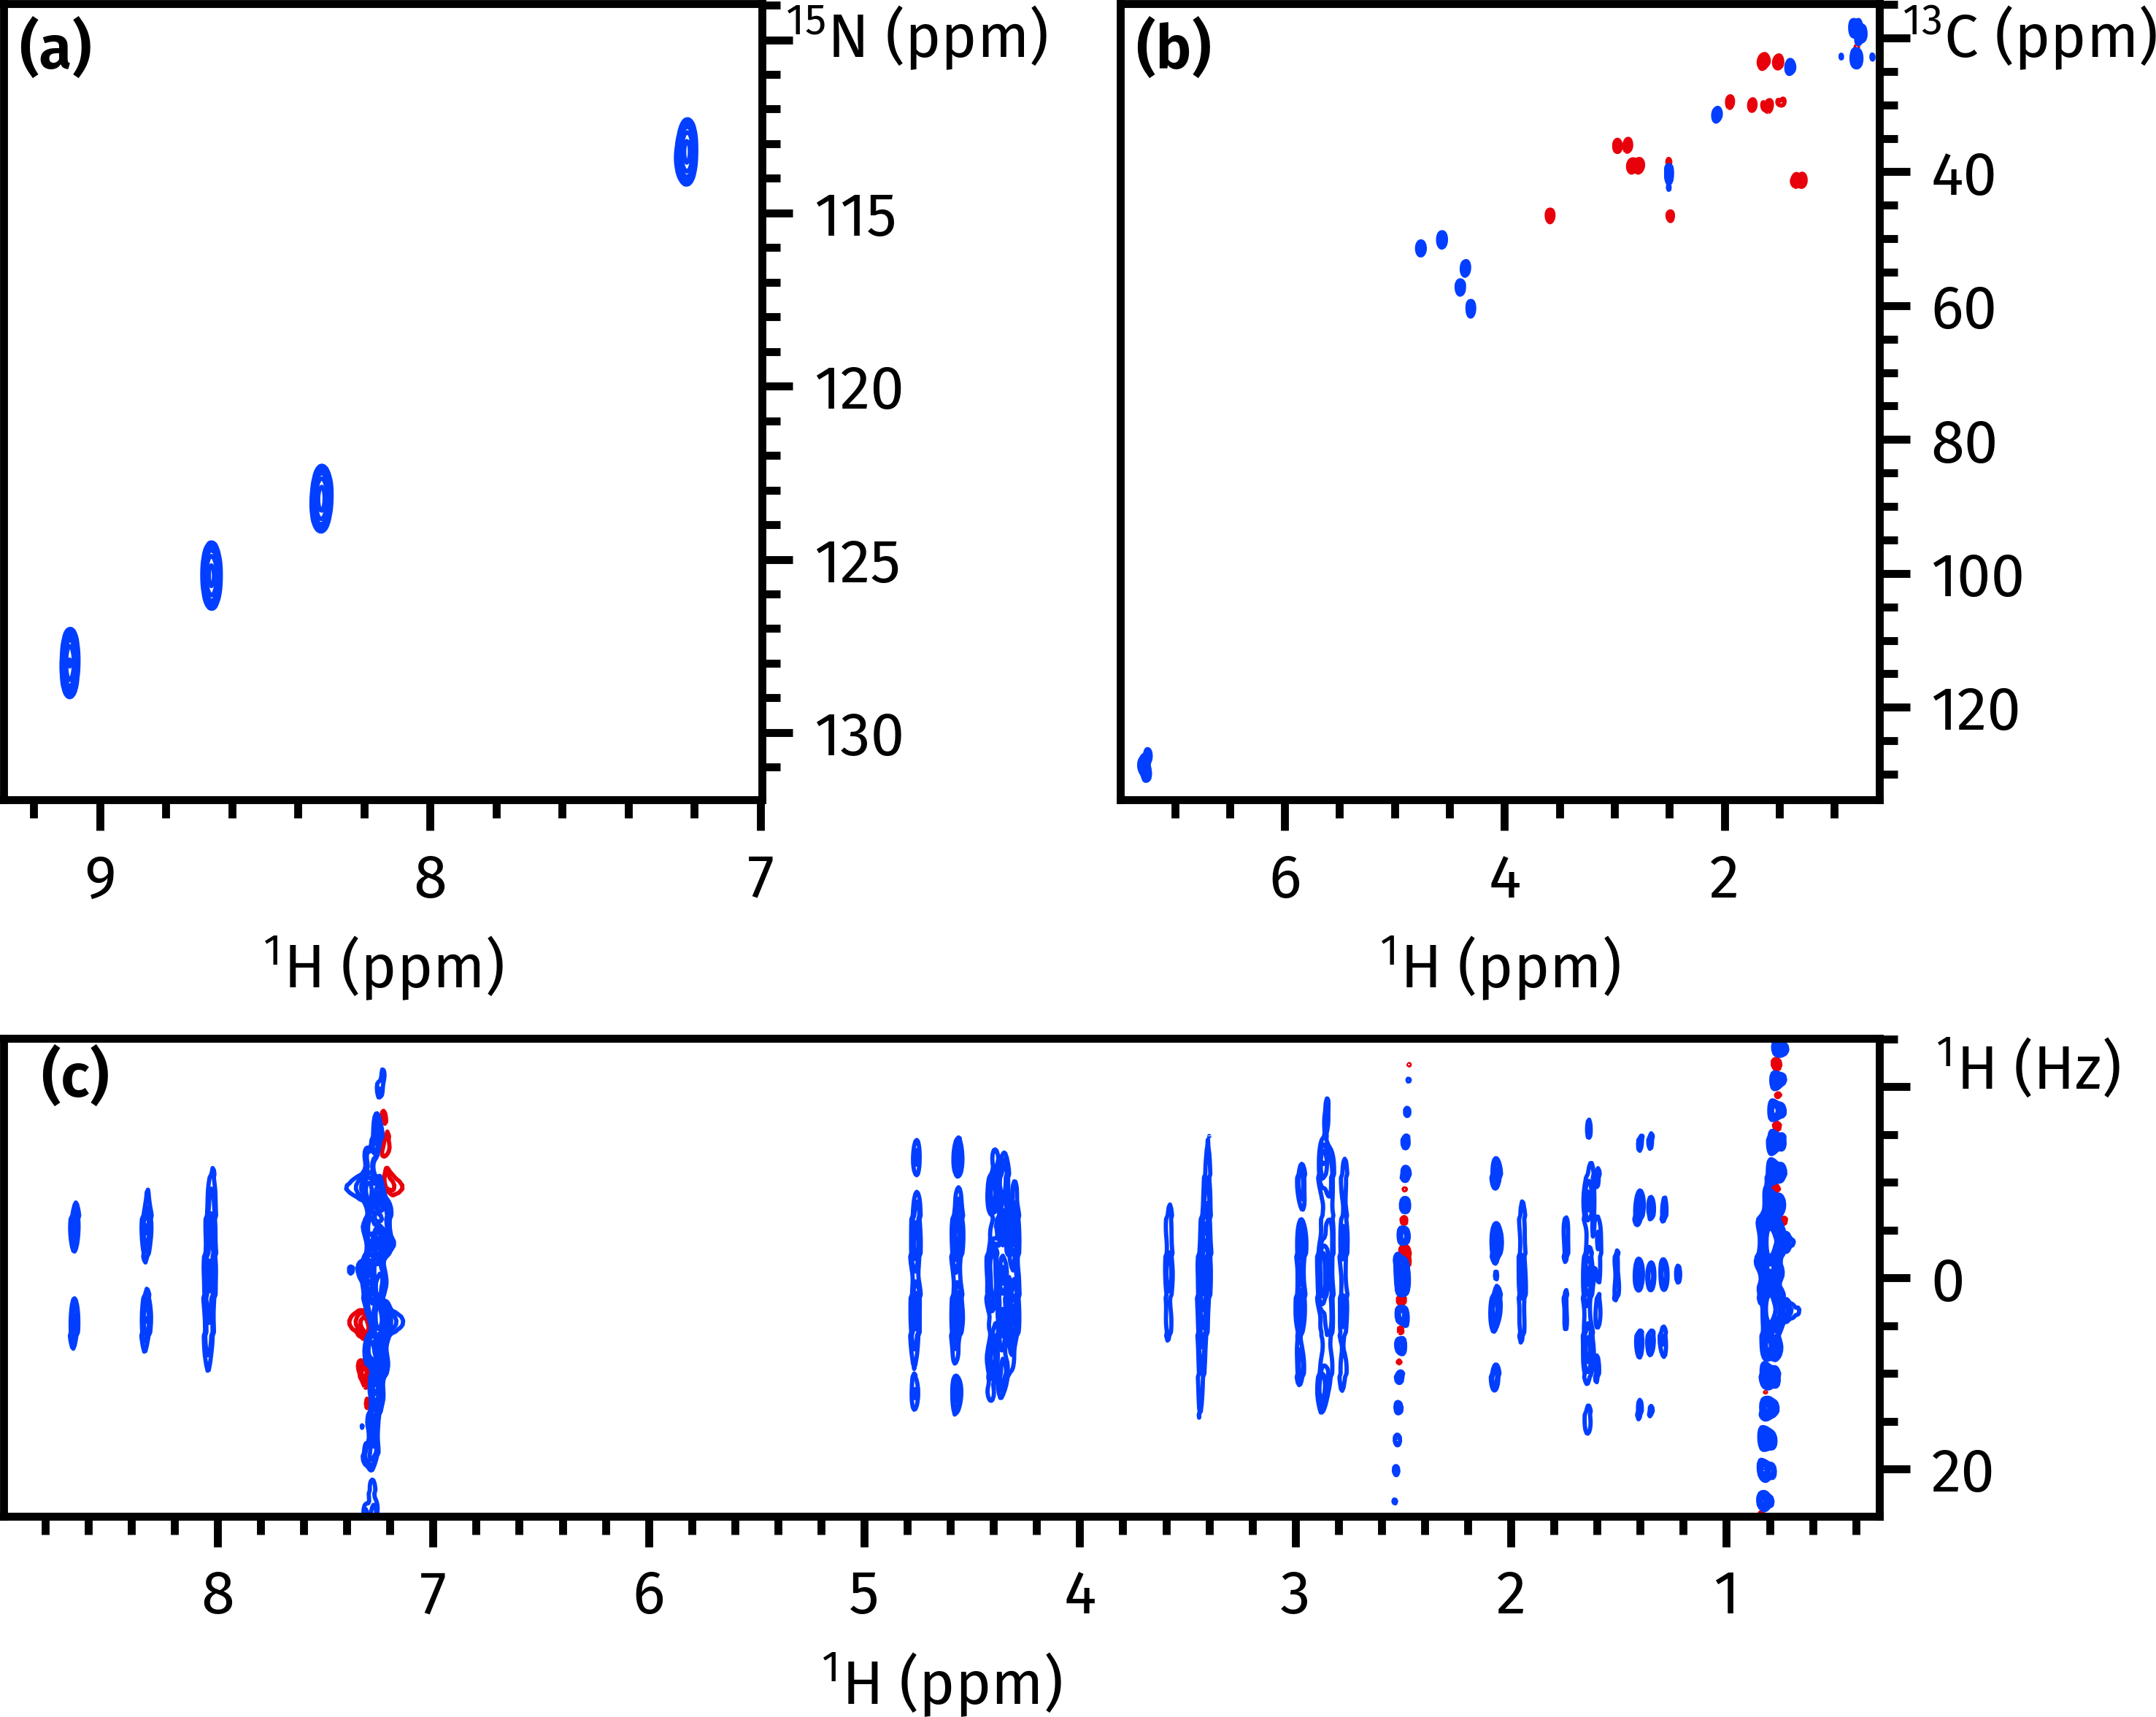
\includegraphics[]{noah/2dj_example.png}%
    {\phantomsubcaption\label{fig:2dj_example_spn}}%
    {\phantomsubcaption\label{fig:2dj_example_spc}}%
    {\phantomsubcaption\label{fig:2dj_example_j}}%
    \caption[Spectra from a \noah{Spn,Sp,J} supersequence]{
        Spectra obtained from a \noah{Spn,Sp,J} supersequence.
        \textbf{(\subref*{fig:2dj_example_spn})} \nitrogen{} seHSQC (256 $t_1$ increments and 2 scans per increment).
        \textbf{(\subref*{fig:2dj_example_spc})} \carbon{} seHSQC.
        \textbf{(\subref*{fig:2dj_example_j})} PSYCHE 2DJ (32 $t_1$ increments and 8 scans per increment).
        \datacode{7G-201028}
    }
    \label{fig:2dj_example}
\end{figure}

The modules thus implemented include the standard magnitude-mode 2DJ experiment, the PSYCHE 2DJ experiment\autocite{Foroozandeh2015CC}, the original 1D PSYCHE\autocite{Foroozandeh2014ACIE}, and the 1D TSE-PSYCHE\autocite{Foroozandeh2015CC}.
An example of the data thus obtained (with the PSYCHE 2DJ) is shown in \cref{fig:2dj_example}.
One particular advantage of including PSYCHE-type modules in NOAH supersequences is that sensitivity is not likely to be at a premium: this is partly because of the increased number of scans, but also partly because other 2D experiments have comparably low sensitivity (meaning that in the time needed to acquire a HSQC, for example, the PSYCHE experiment will also have sufficient sensitivity).
This allows the user to choose a relatively small flip angle (ca.\ \ang{10}) for the PSYCHE saltire pulses in order to minimise artefacts from imperfect decoupling.

On top of that, for the 1D (TSE-)PSYCHE sequences, the extra transients can be used to perform SAPPHIRE averaging\autocite{Moutzouri2017CC}: in this procedure, each chunk of the pure shift interferogram is collected multiple times while varying the point in time where the J-couplings are perfectly refocused.
Summation of these data leads to the suppression of artefacts which arise due to the periodic J-modulation in the interferogram.
This averaging is somewhat analogous to a phase cycle, and performing an 8-step SAPPHIRE averaging procedure (for example) would often require the experiment to be lengthened beyond the duration which is truly necessary: however, in the context of NOAH this is obtained essentially `for free'.
In the GENESIS pulse programmes, this feature is enabled by default (it can be turned off by selecting the original modules using developer mode).

\begin{figure}[!ht]
    \centering
    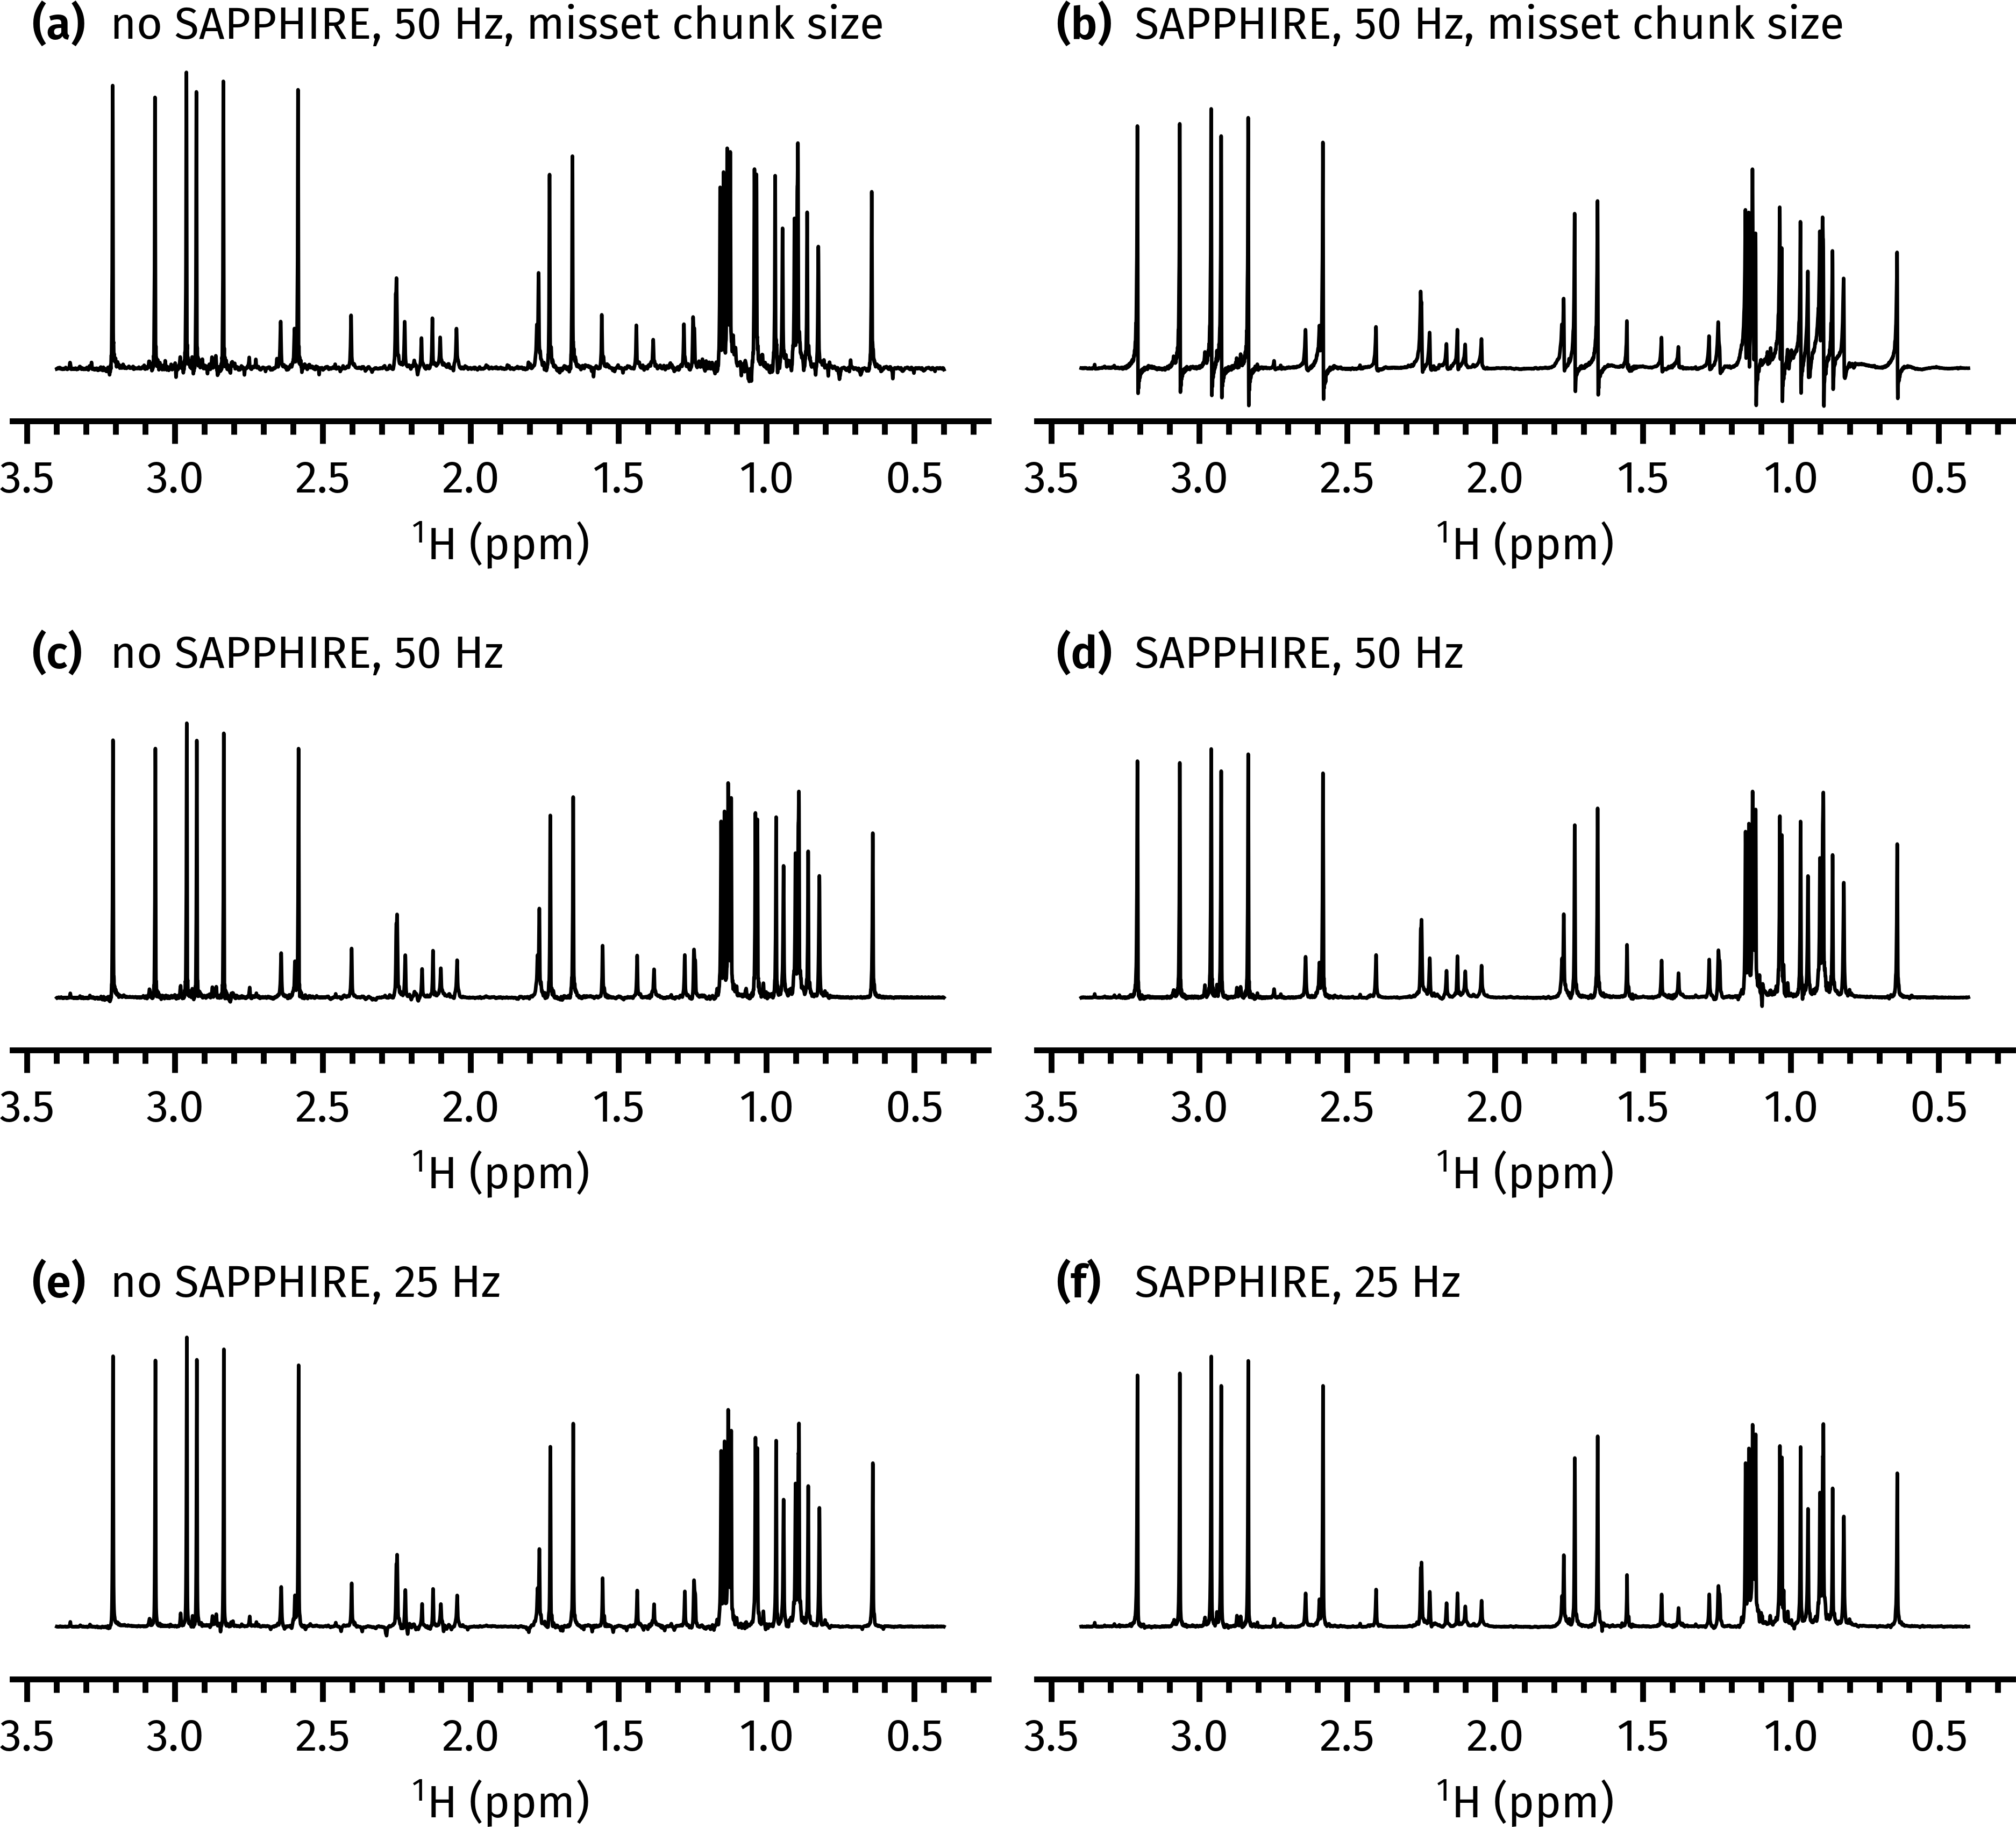
\includegraphics[]{noah/psyche_wrongsw1.png}%
    {\phantomsubcaption\label{fig:psyche_wrongsw1_bad_nosap}}%
    {\phantomsubcaption\label{fig:psyche_wrongsw1_bad_sap}}%
    {\phantomsubcaption\label{fig:psyche_wrongsw1_good_nosap}}%
    {\phantomsubcaption\label{fig:psyche_wrongsw1_good_sap}}%
    \caption[Effect of missetting the chunk size in PSYCHE spectra]{
        A series of 1D PSYCHE spectra obtained from the \noah{Spn,Sp,P} supersequence (saltire flip angle of \ang{15}).
        \textbf{(\subref*{fig:psyche_wrongsw1_bad_nosap})} 1D PSYCHE spectrum acquired without SAPPHIRE averaging and an incorrect chunk size which is not an integral number of complex data points.
        \textbf{(\subref*{fig:psyche_wrongsw1_bad_sap})} 1D PSYCHE spectrum with  8-step SAPPHIRE averaging and an incorrect chunk size; this manifests as phase errors which cannot be corrected.
        \textbf{(\subref*{fig:psyche_wrongsw1_good_nosap})--(\subref*{fig:psyche_wrongsw1_good_sap})} The same as (\subref*{fig:psyche_wrongsw1_bad_nosap}) and (\subref*{fig:psyche_wrongsw1_bad_sap}), but with the chunk size automatically corrected in the pulse programme.
        The impact of the SAPPHIRE averaging is less obvious in these datasets (compare (\subref*{fig:psyche_wrongsw1_good_nosap}) and (\subref*{fig:psyche_wrongsw1_good_sap})), but is more striking when larger chunk sizes are used, as discussed in the original paper\autocite{Moutzouri2017CC}.
        \datacode{7C-211123}
    }
    \label{fig:psyche_wrongsw1}
\end{figure}

A final and more prosaic implementation detail is that in the 1D pure shift modules, the chunk size is automatically rounded to the nearest even multiple of the dwell time $\tau_\text{dw}$ (\texttt{DW} in TopSpin).
This ensures that each chunk consists of an integral number of complex data points.
Although this can be set by the user manually, it is very easy to forget, especially for someone not fully acquainted with the experiment; the results can be quite different, as illustrated in \cref{fig:psyche_wrongsw1}.
When an $n$-step SAPPHIRE averaging is used, the requirement is even stricter: the chunk size must be a multiple of $2n \tau_\text{dw}$.
This is also encoded in the pulse programmes.

\subsection{HMBC}
\label{subsec:noah__hmbc}

The HMBC module is one which in fact does not fit perfectly into the NOAH principle of only exciting magnetisation which is needed.
As described in \cref{subsec:noah__case_studies}, the HMBC module should only require magnetisation of protons which have long-range couplings to \carbon{}; however, it ends up exciting \textit{all} \magnnot{C} magnetisation.
This leads to sharply reduced, and also unbalanced, intensities of homonuclear modules which come later in the supersequences.

I made some early (and brief) attempts at devising a pulse sequence which sought to discriminate these two magnetisation components using a perfect echo\autocite{Parella2019MRC}.
However, this was quickly abandoned as it proved very difficult to \textit{also} retain \magn{C} magnetisation.
I do not claim here that it is impossible to come up with a pulse sequence which does this, but it is certainly not easy, and ultimately I turned my focus to improving (rather than replacing) the HMBC module.


\subsubsection{Suppression of one-bond artefacts}

One of the issues with the NOAH HMBC module was that there were an unusual amount of one-bond artefacts, which arise from \magn{C} magnetisation that is allowed to evolve during the pulse sequence.
Generally, HMBC experiments seek to suppress this through the use of a low-pass J-filter (LPJF, see also \cref{subsec:poise__hmbc}).
The NOAH HMBC module \textit{additionally} contains a $zz$-filter, which stores \magn{C} magnetisation along $+z$ before the LPJF.
Thus, in theory, one-bond artefacts should be suppressed in the NOAH HMBC to an even greater extent.

However, this expectation is not borne out: in some cases, the NOAH HMBC has \textit{more intense} one-bond artefacts when compared against a standard HMBC experiment (\cref{fig:noah_hmbc_1jch_no90,fig:noah_hmbc_1jch_std_lp2}).
Even performing a POISE optimisation of the LPJF delays, as described in \cref{subsec:poise__hmbc}, did not lead to any reduction in artefacts.
I hypothesised instead that these artefacts arose from imperfect manipulation of \magn{C} magnetisation by the $zz$-filter.
In particular, any \textit{antiphase} magnetisation (of the form $I_xS_z$ or $I_yS_z$) generated after the $zz$-filter would be reconverted into in-phase $I_x$ or $I_y$ terms, which would not be destroyed by the LPJF.%
\footnote{It would be nice to back this up with simulations, but I did not have the time to run these.}
(The LPJF works based on the assumption that it needs to destroy in-phase magnetisation, which is true if the excitation element is just a \proton{} \ang{90} pulse, but is not necessarily applicable in the NOAH HMBC.)

Such antiphase terms can, however, be easily removed by the addition of a \carbon{} \ang{90} pulse, which transforms them into a mixture of double- and zero-quantum terms: these are either unobservable, or can be efficiently dephased by CTP gradients.
This technique is used in the CLIP-HSQC family of experiments\autocite{Enthart2008JMR,Gyongyosi2021AC}, as well as the LPJF itself.
In this case, we simply need to add an additional \carbon{} \ang{90} pulse between the $zz$-filter and the LPJF: this pulse is highlighted in \cref{fig:noah_sb_po_b}.
This results in a striking reduction of the one-bond artefacts, as shown in \cref{fig:noah_hmbc_1jch_90}.
The suppression accomplished with the addition of this \ang{90} pulse is superior to that in the standard HMBC (\cref{fig:noah_hmbc_1jch_std_lp2}), and is comparable to a standard HMBC with a third-order LPJF (\cref{fig:noah_hmbc_1jch_std_lp3}).
Of course, the NOAH module---which by default uses a second-order LPJF---can also be `upgraded' to use a third-order LPJF.
In GENESIS pulse programmes, this can be done using the \texttt{-DLP3} acquisition flag (although the results were not evaluated here).

\begin{figure}[!ht]
    \centering
    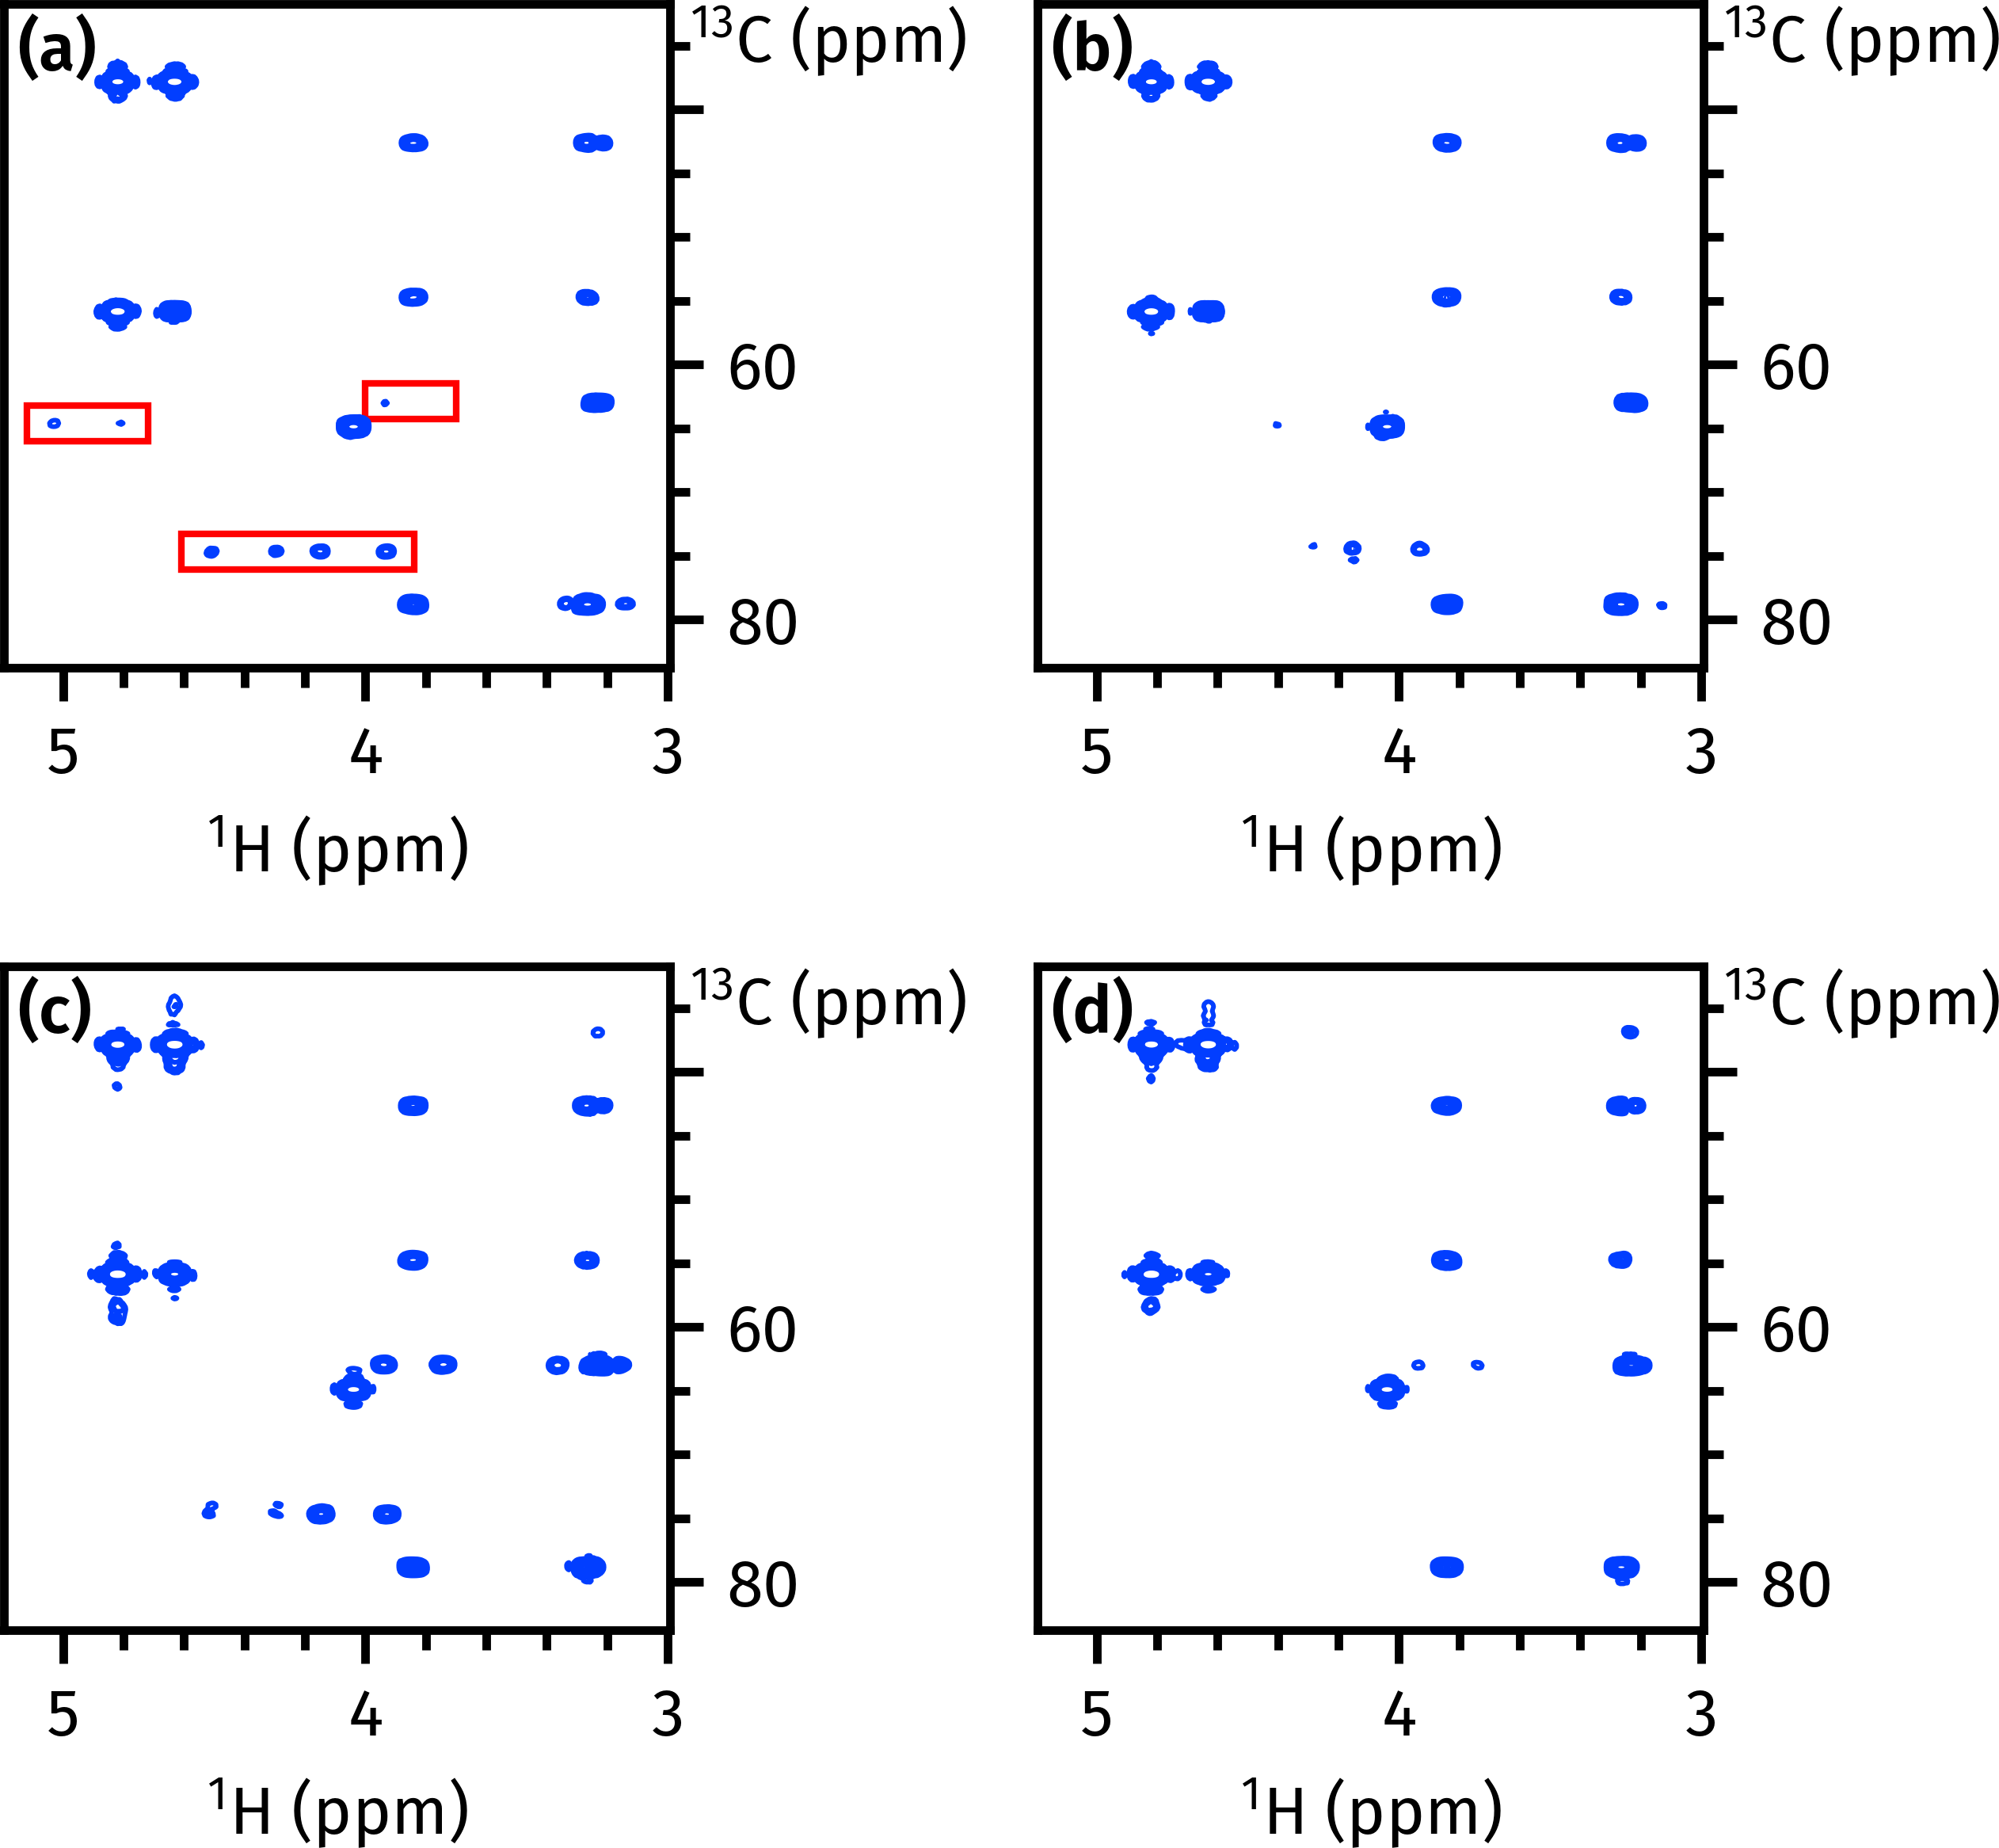
\includegraphics[]{noah/hmbc_1jch.png}%
    {\phantomsubcaption\label{fig:noah_hmbc_1jch_no90}}%
    {\phantomsubcaption\label{fig:noah_hmbc_1jch_90}}%
    {\phantomsubcaption\label{fig:noah_hmbc_1jch_std_lp2}}%
    {\phantomsubcaption\label{fig:noah_hmbc_1jch_std_lp3}}%
    \caption[Suppression of one-bond artefacts in NOAH HMBC spectra]{
        \textbf{(\subref*{fig:noah_hmbc_1jch_no90})} NOAH $zz$-HMBC module without the additional \ang{90} pulse.
        One-bond artefacts are highlighted in red.
        \textbf{(\subref*{fig:noah_hmbc_1jch_90})} NOAH $zz$-HMBC with the \ang{90} pulse.
        \textbf{(\subref*{fig:noah_hmbc_1jch_std_lp2})} Standard library HMBC with a second-order LPJF.
        \textbf{(\subref*{fig:noah_hmbc_1jch_std_lp3})} Standard library HMBC with a third-order LPJF.
        \datacode{7A-210916}
    }
    \label{fig:noah_hmbc_1jch}
\end{figure}


\subsubsection{Gradient selection schemes}

Another point which was investigated (but bore less fruit) was the gradient scheme used for CTP selection.
The NOAH module, as shown in \cref{fig:noah_sb_po_b}, uses a `symmetric' scheme where two gradients of equal amplitude surround the $t_1$ period: this encoding is later decoded by a third gradient just prior to acquisition.
However, other choices exist: for example, the Bruker standard library HMBC (derived from the work of Cicero et al.\autocite{Cicero2001JMR}) uses only two gradients which have unequal amplitudes.
This gradient scheme cannot be directly used in a NOAH HMBC module, though.
This is because the $zz$-filter element places \magn{C} magnetisation along the $+z$ axis just before the HMBC J-evolution delay (see \cref{fig:noah_sb_po_b}).
This magnetisation later experiences the \proton{} \ang{180} pulse in the middle of $t_1$, which means that an extra \ang{180} pulse must be added at the very end of the sequence to finally return it to $+z$.
It is necessary to ensure that there is at least one gradient placed after this \ang{180} pulse to ensure proper CTP selection (in the `symmetric' scheme of \cref{fig:noah_sb_po_b}, this is fulfilled by the gradient $g_2$).

\begin{figure}[!htbp]
    \centering
    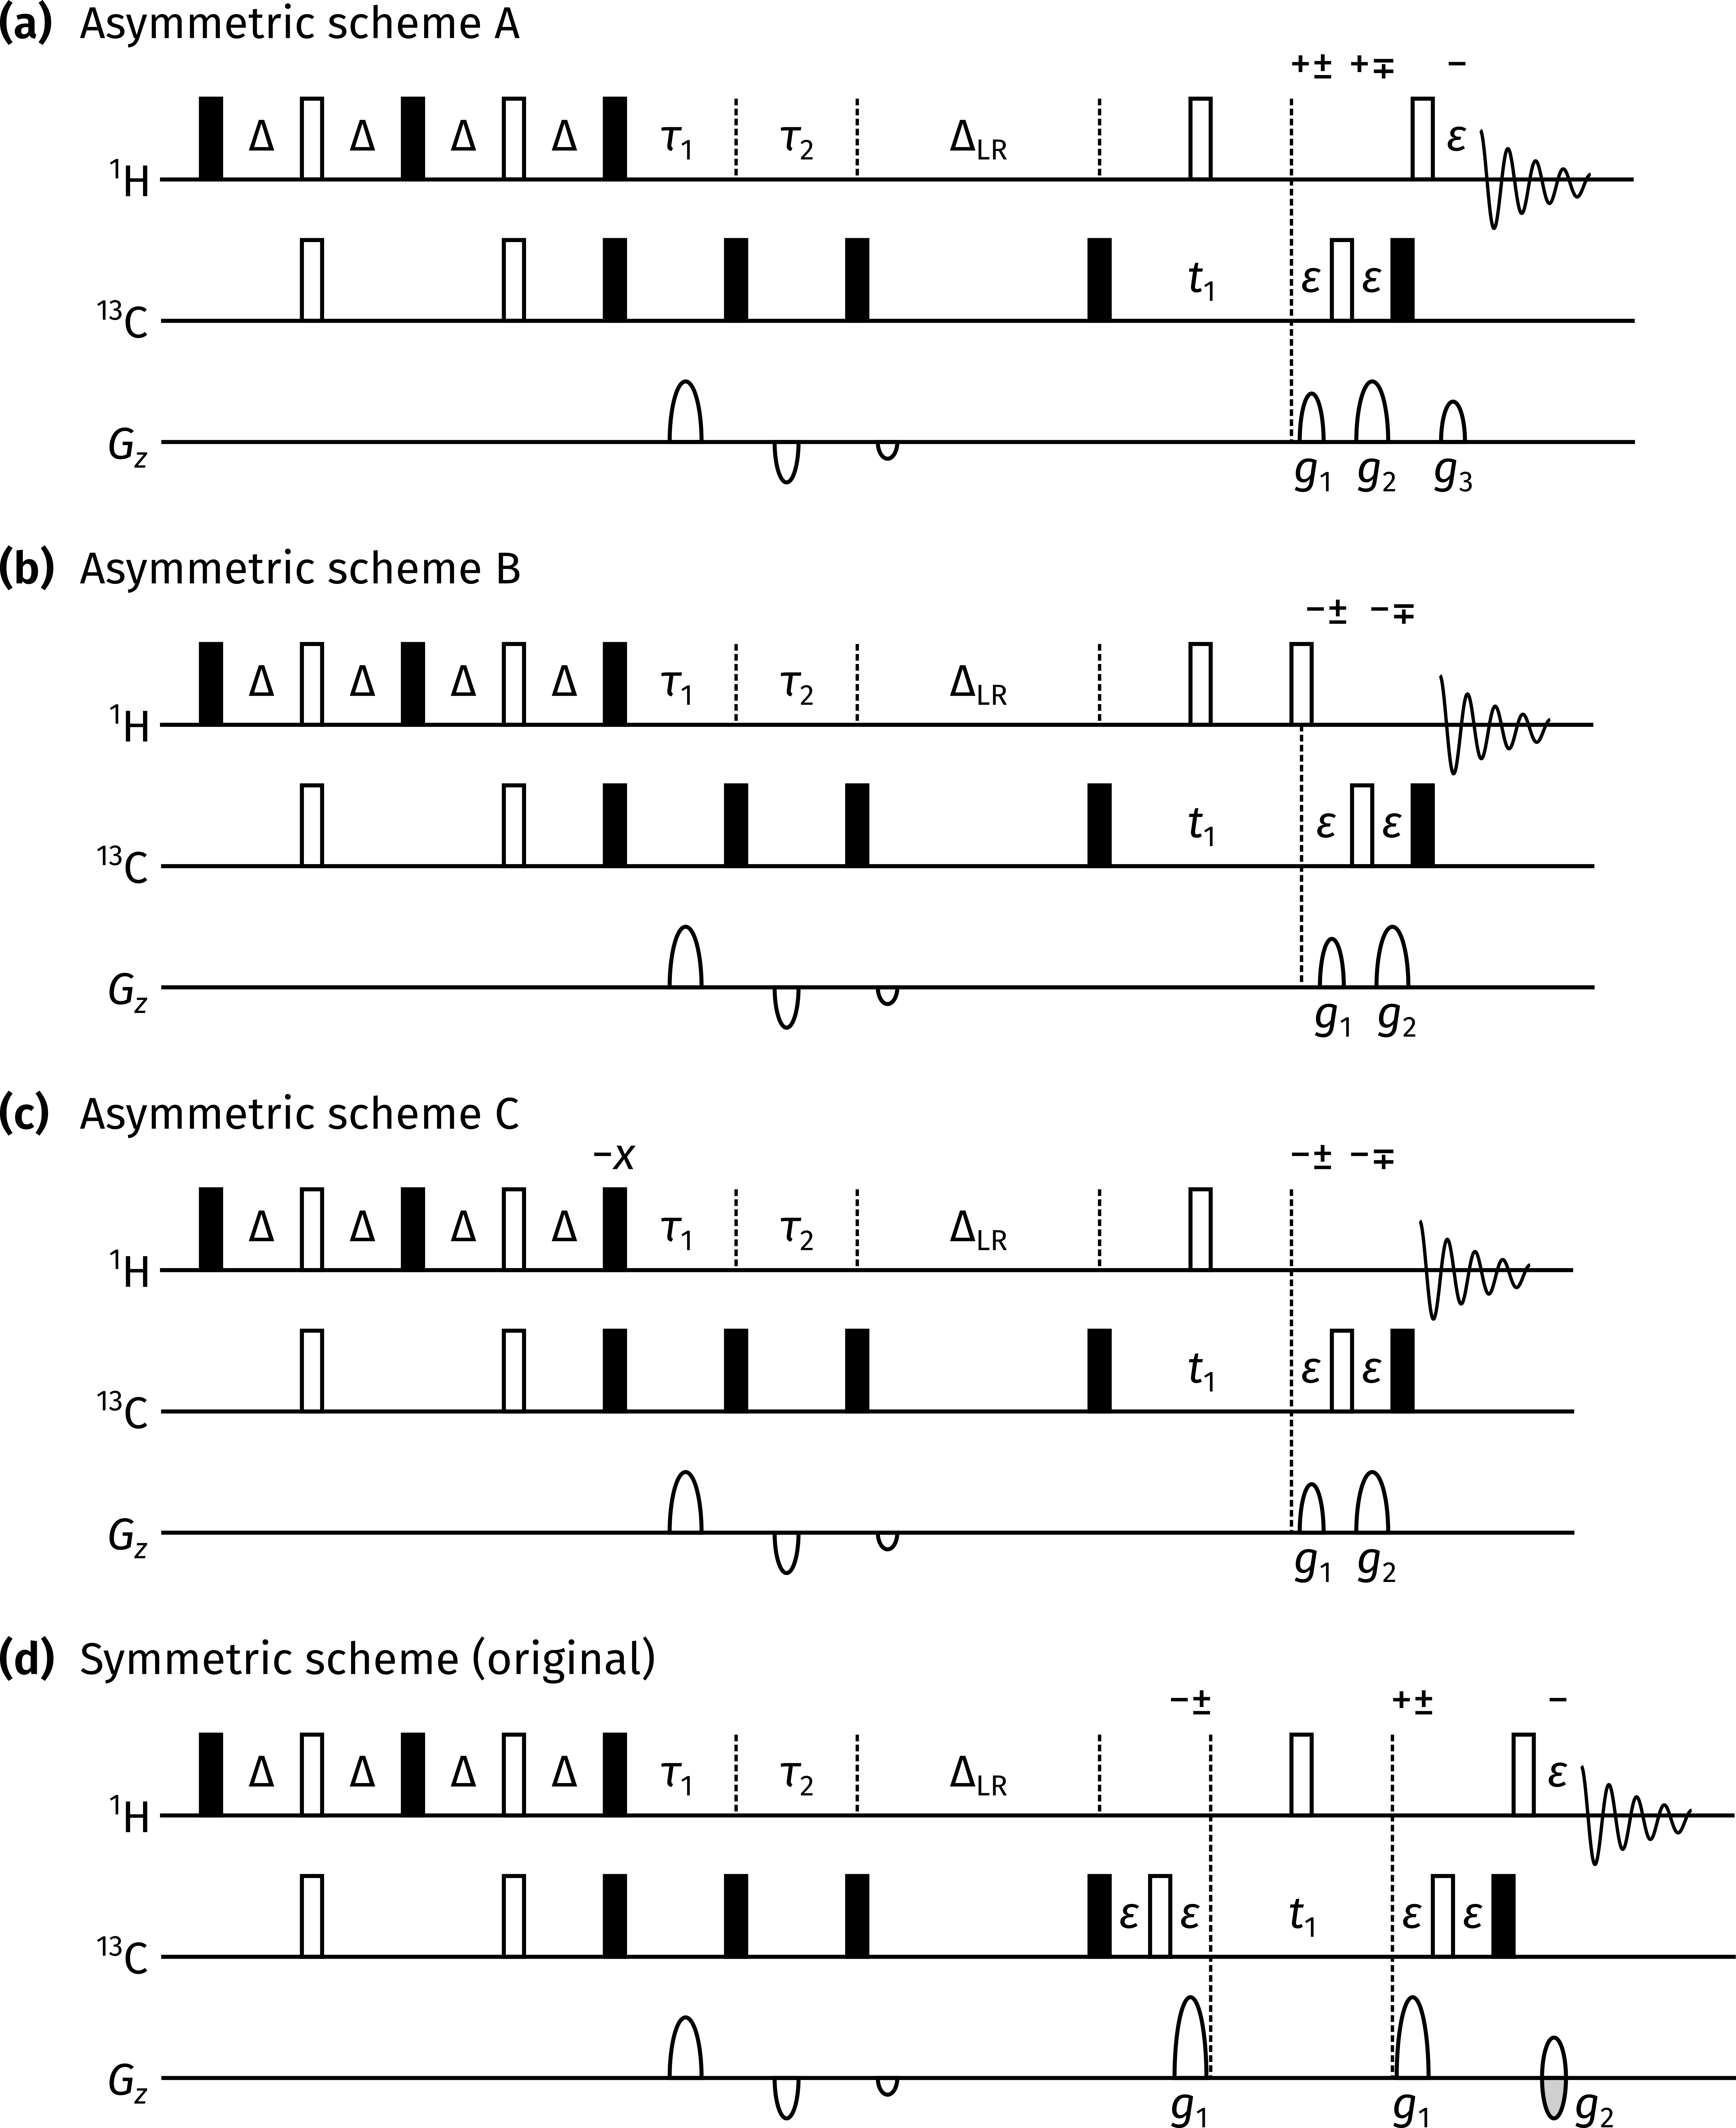
\includegraphics[]{pp/hmbc/noah_grads.png}%
    {\phantomsubcaption\label{fig:noah_hmbc_grads_bga}}%
    {\phantomsubcaption\label{fig:noah_hmbc_grads_bgb}}%
    {\phantomsubcaption\label{fig:noah_hmbc_grads_bgc}}%
    {\phantomsubcaption\label{fig:noah_hmbc_grads_b}}%
    \caption[Alternative CTP gradient schemes investigated for NOAH HMBC]{
        Alternative CTP gradient schemes investigated for the NOAH HMBC module.
        The coherences selected for during each gradient are indicated above each gradient, using the same notation for product operators as described in the \textit{Preface}: the `upper' term (e.g.\ $+$ in $\pm$) refers to the echo experiment, and the `lower' term to the antiecho experiment.
        So, for example, $+\pm$ refers to selection of $I_+S_+$ during the echo experiment and $I_+S_-$ during the antiecho experiment.
        Gradient amplitudes are as described in the text.
        \textbf{(\subref*{fig:noah_hmbc_grads_bga})} `Asymmetric scheme A', modified from the standard library sequence to include an additional \ang{180} pulse and gradient.
        \textbf{(\subref*{fig:noah_hmbc_grads_bgb})} `Asymmetric scheme B', where the \ang{180} pulse is shifted forward to the end of $t_1$.
        \textbf{(\subref*{fig:noah_hmbc_grads_bgc})} `Asymmetric scheme C', which modifies the $zz$-filter instead of using an extra \ang{180} pulse.
        \textbf{(\subref*{fig:noah_hmbc_grads_b})} The original `symmetric' scheme (the same as in \cref{fig:noah_sb_po_b}), placed here for convenience.
    }
    \label{fig:noah_hmbc_grads}
\end{figure}

Using this knowledge, it is possible to construct several `asymmetric' gradient schemes:
\begin{enumerate}
    \item `Scheme A' (\cref{fig:noah_hmbc_grads_bga}) is modified from the Bruker standard library to include a \ang{180} pulse and gradient at the end.
        The presence of an additional gradient means that there is a free parameter, here denoted as $\alpha$, which can be used to control the relative amplitudes of these three CTP gradients.
        The gradient amplitudes are chosen as follows:
        \begin{align}
            &\text{echo:}     & g_1 &= gc_1 & g_2 &= g    & g_3 &= gc_2 \label{eq:noah_hmbc_grads_bga_echo} \\
            &\text{antiecho:} & g_1 &= g    & g_2 &= gc_1 & g_3 &= gc_2 \label{eq:noah_hmbc_grads_bga_antiecho}
        \end{align}
        where $c_1 = -\alpha(\gammaH - \gammaC)/(\gammaH + \gammaC)$ and $c_2 = (1 - \alpha) (\gammaH - \gammaC)/\gammaH$.
        In principle $g$ is also a free parameter; for maximum suppression of artefacts I chose a relatively large value of 80\%.
    \item In `Scheme B' (\cref{fig:noah_hmbc_grads_bgb}), the \ang{180} pulse is shifted to immediately after $t_1$, before any of the CTP gradients have been applied. This means that there is no need for a third gradient, and the CTP gradient amplitudes can be directly taken from the standard library sequence:
        \begin{align}
            &\text{echo:}     & g_1 &= g  & g_2 &= gc \label{eq:noah_hmbc_grads_bgb_echo} \\
            &\text{antiecho:} & g_1 &= gc & g_2 &= g \label{eq:noah_hmbc_grads_bgb_antiecho}
        \end{align}
        where $c = -(\gammaH - \gammaC)/(\gammaH + \gammaC)$ and $g = 80\%$.
    \item `Scheme C' (\cref{fig:noah_hmbc_grads_bgc}) simply does not add a \ang{180} pulse, but instead modifies the phases of the $zz$-filter in order to place \magn{C} magnetisation along the $-z$ axis during the HMBC J-evolution delay.
        Here, the gradient amplitudes are the same as those in the standard library sequence as well as in scheme B.
\end{enumerate}

It is of interest to note two limiting cases of scheme A.
When $\alpha = (\gammaH + \gammaC)/(\gammaH - \gammaC) \approx 1.67$, we obtain the ratio $g_1 : g_2 : g_3 = 1 : -1 : \pm 2\gammaC/\gammaH$, which mimics the original `symmetric' scheme (\cref{fig:noah_hmbc_grads_b}); and when $\alpha = 1$, we have that $g_3 = 0$, i.e.\ a return to the two-gradient tactic of schemes B and C.
In the tests which follow, I ran scheme A with $\alpha = 1.67$, $\alpha = 0.6$, and $\alpha = 0.3$.

\begin{figure}[htb]
    \centering
    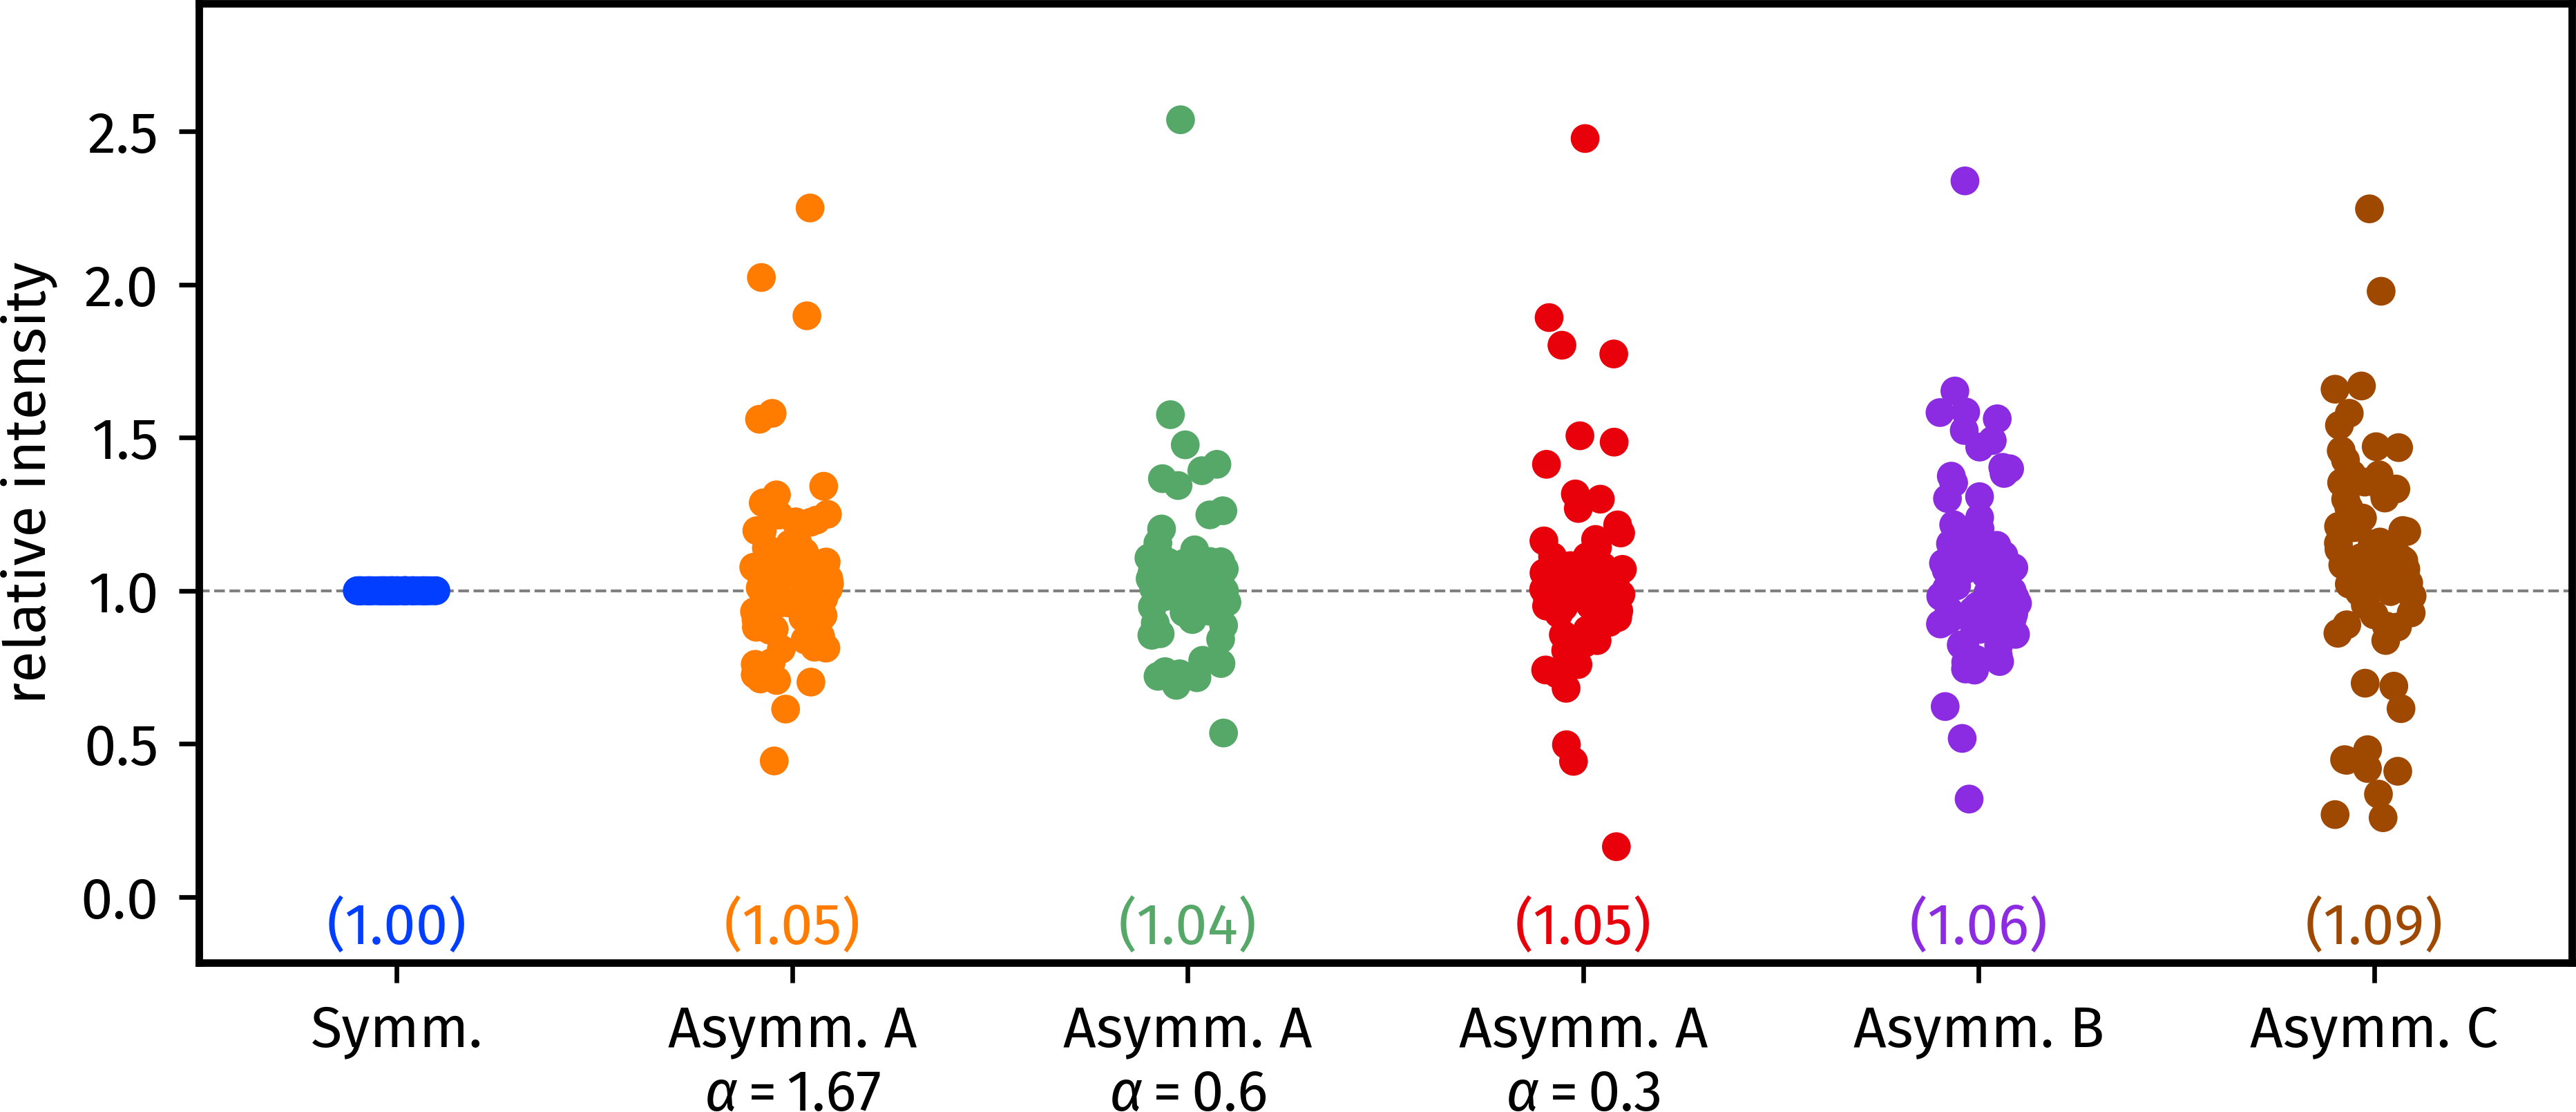
\includegraphics[]{noah/hmbc_grad_sens.png}%
    \caption[Comparison of relative sensitivities of HMBC gradient schemes]{
        Sensitivities of various asymmetric HMBC gradient schemes, as compared to the symmetric scheme in \cref{fig:noah_sb_po_b}.
        Each dot indicates one crosspeak in the HMBC spectrum; the numbers in parentheses are the average over all peaks.
        \datacode{7A-211226}
    }
    \label{fig:hmbc_grad_sens}
\end{figure}

All of the different HMBC versions above, plus the original `symmetric' scheme in \cref{fig:noah_sb_po_b}, were tested in the context of a \noah{B,S} supersequence using the andrographolide sample (\cref{fig:hmbc_grad_sens}).
As can be seen, there is not much at all which separates the different versions (outliers with $>2\times$ `sensitivity improvements' can be attributed to different J-modulation in the multiplet).
The most sensitive of these is asymmetric scheme C, which may be explained by the fact that it has one fewer \ang{180} pulse: however, this comes with an immediate drawback.
Since scheme C places the \magn{C} magnetisation along $-z$ during the LPJF as well as the J-evolution delay $\Delta_\text{LR}$ (a total of ca.\ \qty{70}{\ms}), relaxation losses during this period lead to poorer retention of \magn{C} magnetisation for later modules, as shown by the decreased HSQC sensitivities in \cref{fig:hmbc_grad_sens_hsqc}.
In contrast, all the other gradient schemes retain \magn{C} magnetisation equally well.

\begin{figure}[htb]
    \centering
    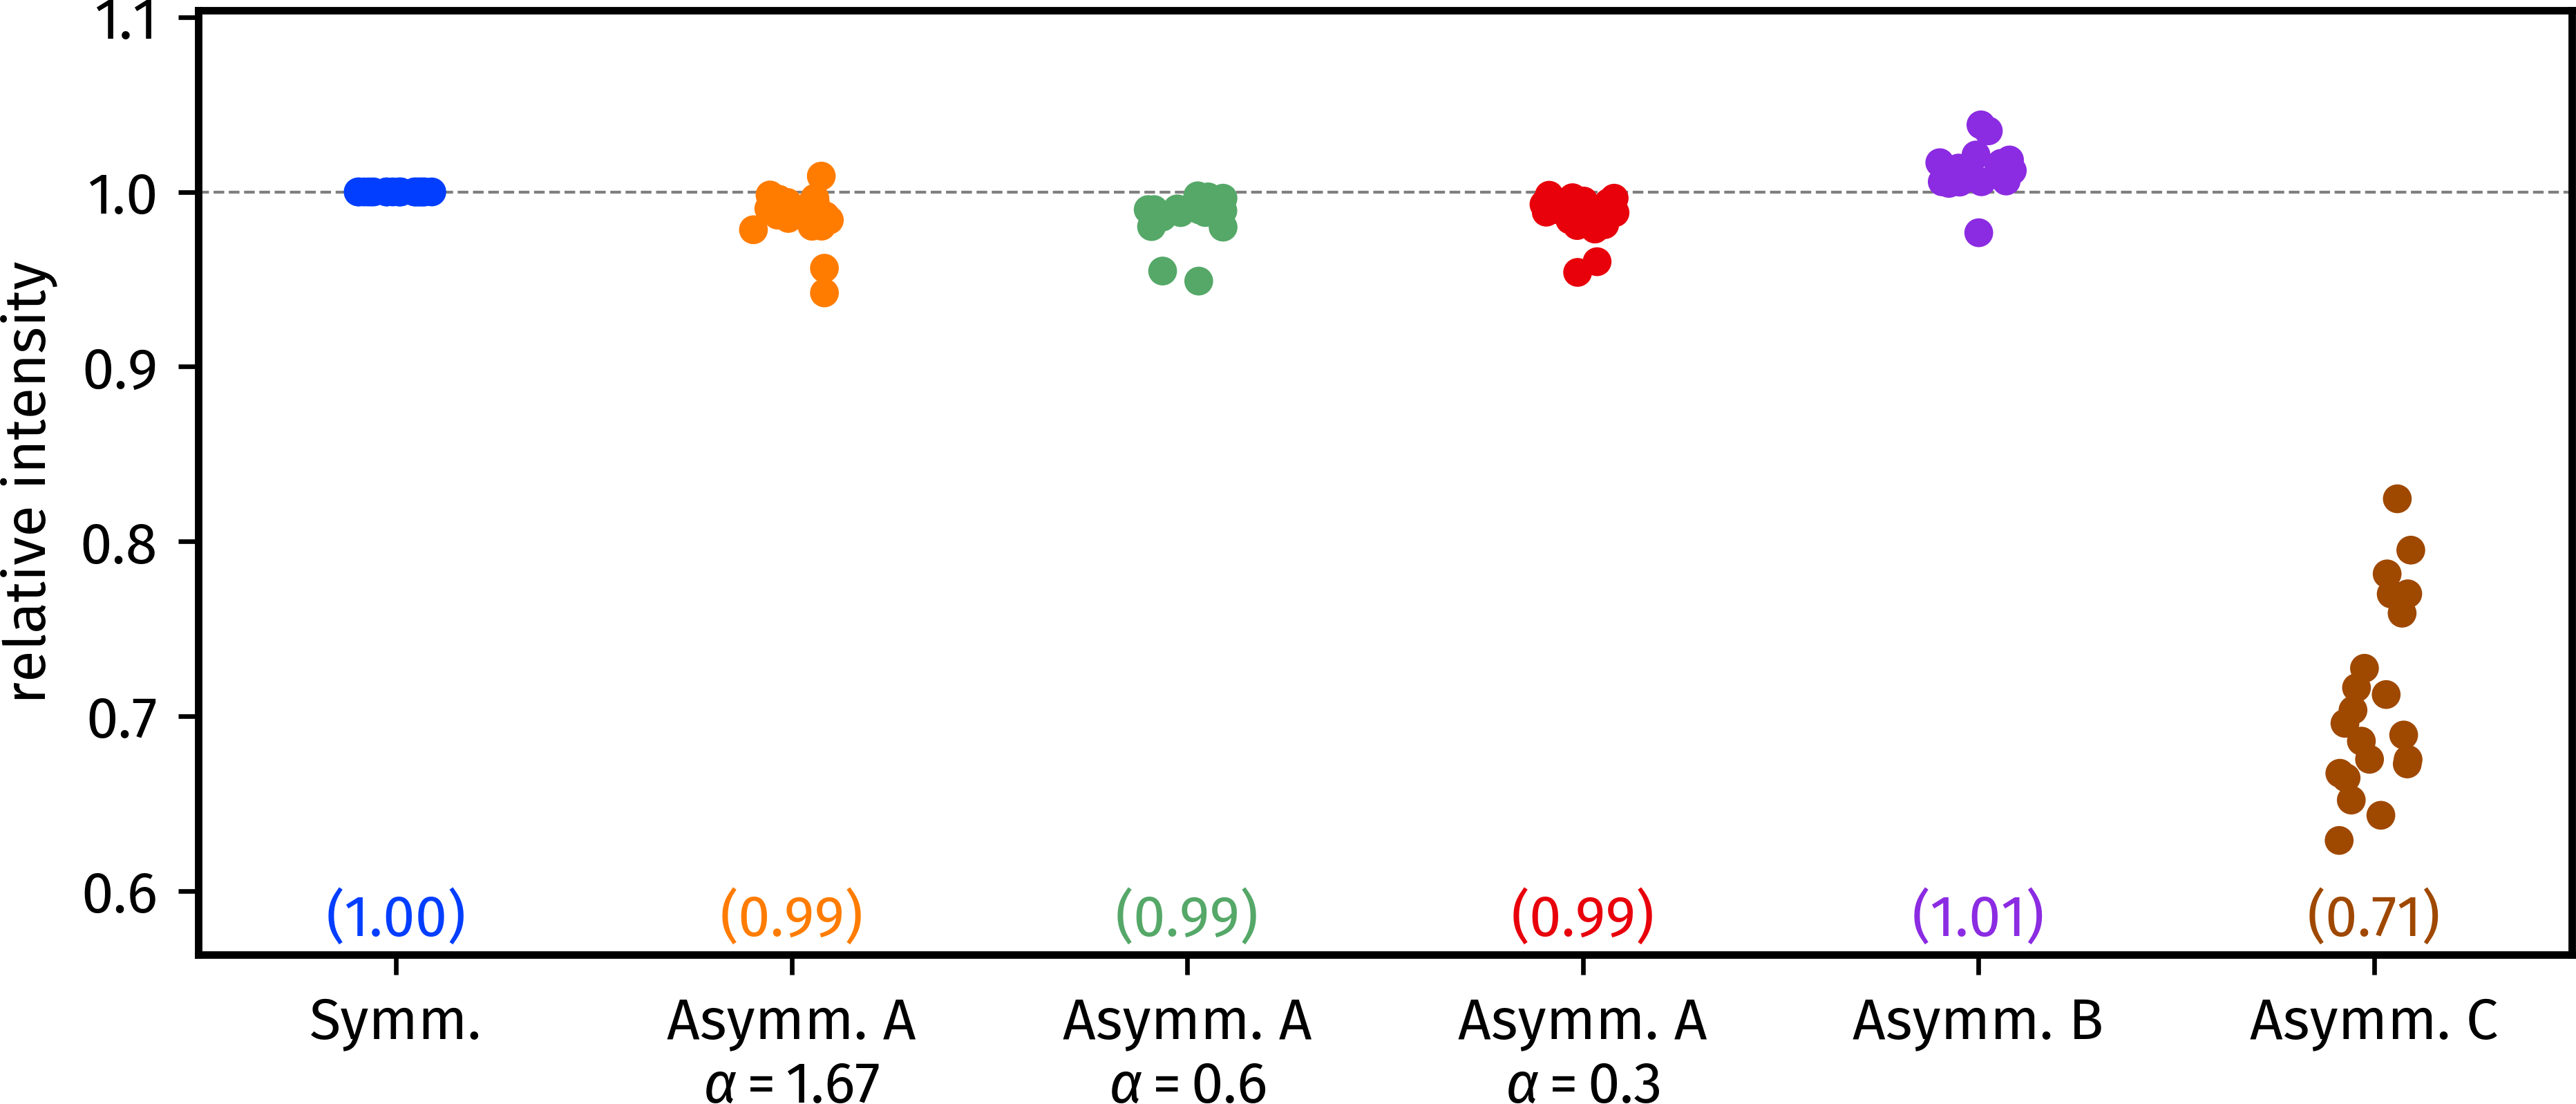
\includegraphics[]{noah/hmbc_grad_sens_hsqc.png}%
    \caption[Effect of HMBC gradient scheme on HSQC sensitivity in a \noah{B,S} supersequence]{
        Sensitivities of the HSQC module in a \noah{B,S} supersequence, where the HMBC module is implemented using the gradient schemes of \cref{fig:hmbc_grad_sens}.
        \datacode{7A-211226}
    }
    \label{fig:hmbc_grad_sens_hsqc}
\end{figure}

The final point worth studying is the quality of the HMBC spectrum itself.
To do this, we need to look at the actual spectra (\cref{fig:hmbc_grad_spec}).
For the most part, the spectra are all the same; however, there is a notable set of artefacts present in \cref{fig:hmbc_grad_spec_asymma1} (scheme A with $\alpha = 1.67$) as well as \cref{fig:hmbc_grad_spec_asymmb} (scheme B), highlighted in red boxes.
These artefacts occur at the frequencies
\begin{equation}
    \label{eq:hmbc_wing_artefacts}
    (\Omega_1, \Omega_2) = \left(\Omega_S \pm \frac{\Omega_I}{2}, \Omega_I\right),
\end{equation}
and are in fact `wing' artefacts similar to that observed in other modules (\cref{subsec:noah__sehsqc_c,subsec:noah__hmqc,subsec:noah__sehsqc_n}).
In this case, they arise due to imperfect refocusing of the \proton{} chemical shift during $t_1$: specifically, whenever $I_zS_\pm$ terms are present during the second half of $t_1$.
Extra evidence for the origin of these artefacts comes from the observation that when the \ang{180} pulse in the middle of $t_1$ is phase cycled, the artefacts are removed.
In a standard HMBC, these terms would not be detected in the final FID; however, in this case, the addition of an extra \ang{180} pulse after $t_1$ provides an opportunity for these to be converted back into observable spin-$I\/$ magnetisation (through off-resonance effects or miscalibration).

The poorer performance may therefore be understood as follows:
when scheme A is acquired with $\alpha = 1.67$, the gradients $g_1$ and $g_2$ have equal and opposite amplitudes, and so do not enforce any coherence selection on spin $I\/$ during the second half of $t_1$.
Likewise, scheme B contains no gradients during the second half of $t_1$.

\begin{figure}[htb]
    \centering
    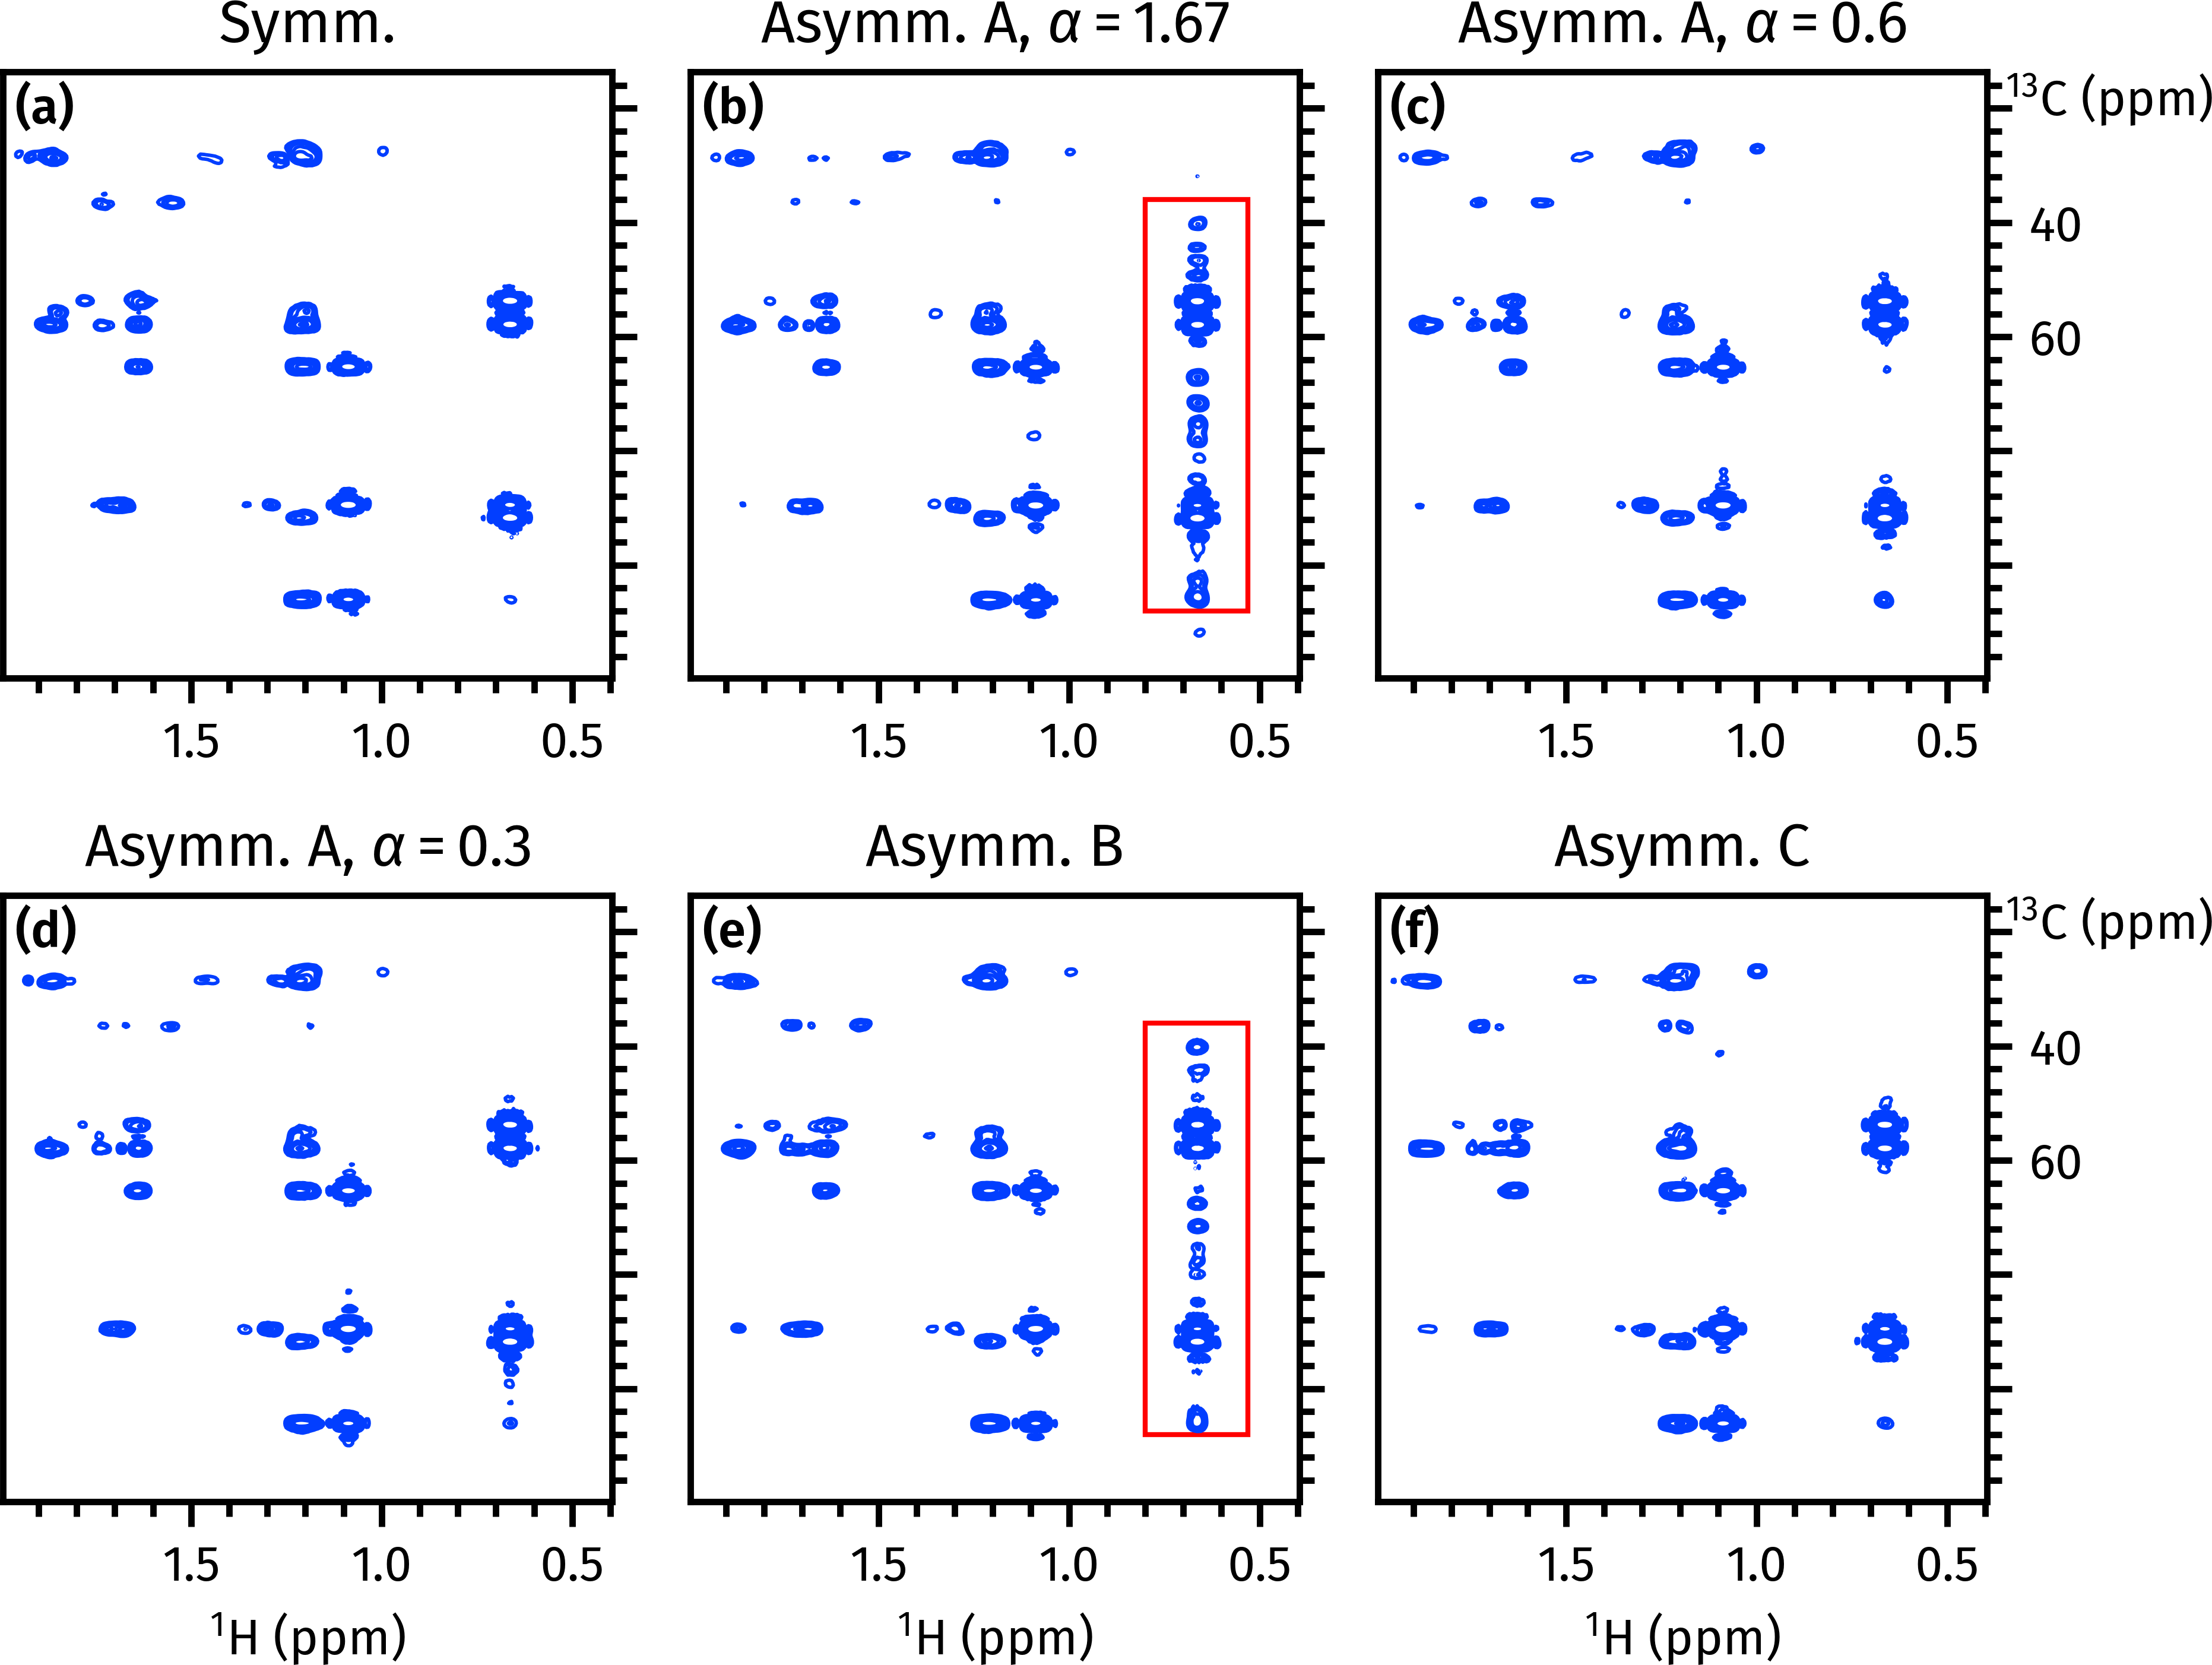
\includegraphics[]{noah/hmbc_grad_spec.png}%
    {\phantomsubcaption\label{fig:hmbc_grad_spec_symm}}%
    {\phantomsubcaption\label{fig:hmbc_grad_spec_asymma1}}%
    {\phantomsubcaption\label{fig:hmbc_grad_spec_asymma2}}%
    {\phantomsubcaption\label{fig:hmbc_grad_spec_asymma3}}%
    {\phantomsubcaption\label{fig:hmbc_grad_spec_asymmb}}%
    {\phantomsubcaption\label{fig:hmbc_grad_spec_asymmc}}%
    \caption[HMBC spectra acquired with different gradient schemes]{
        HMBC spectra acquired with the gradient schemes of \cref{fig:hmbc_grad_sens}.
        Extra `wing' artefacts present in two of the spectra (asymmetric scheme A with $\alpha = 1.67$, \textbf{(\subref*{fig:hmbc_grad_spec_asymma1})}, and asymmetric scheme B, \textbf{(\subref*{fig:hmbc_grad_spec_asymmb})}) are highlighted in red boxes.
        \datacode{7A-211226}
    }
    \label{fig:hmbc_grad_spec}
\end{figure}

The characteristics of these gradient schemes are summarised in \cref{tbl:hmbc_grads}.
As can be seen, the `best' schemes are either the original symmetric scheme, or asymmetric scheme A with $\alpha \neq 1.67$.
However, there is not much difference between these: it is not clear whether the improvement in sensitivity is reproducible across a wide range of samples, and in any case, the gains are extremely marginal.

\begin{table}[htb]
    \begin{tabular}{cccc}
        \toprule
        \textbf{Gradient scheme} & \textbf{HMBC sensitivity} & \textbf{HSQC sensitivity} & \textbf{Wing artefacts} \\
        \midrule
        Symmetric                     & 1    & 1    & No  \\
        Asymmetric A, $\alpha = 1.67$ & 1.05 & 0.99 & Yes \\
        Asymmetric A, $\alpha = 0.6$  & 1.04 & 0.99 & No  \\
        Asymmetric A, $\alpha = 0.3$  & 1.05 & 0.99 & No  \\
        Asymmetric B                  & 1.06 & 1.01 & Yes \\
        Asymmetric C                  & 1.09 & 0.71 & No  \\
        \bottomrule
    \end{tabular}
    \caption[Comparison of HMBC gradient schemes]{
        Comparison of HMBC gradient schemes discussed in this section: the data are a summary of \cref{fig:hmbc_grad_sens,fig:hmbc_grad_sens_hsqc,fig:hmbc_grad_spec}.
        \datacode{7A-211226}
    }
    \label{tbl:hmbc_grads}
\end{table}


\subsubsection{Other artefacts}

It has been established that the HMBC module (and supersequences containing it) are not fully ideal in terms of magnetisation preservation.
However, there are also some other curious phenomena which have not been fully described in the literature.
One of these is the presence of \textit{inverted peaks} in the homonuclear X module(s) in a \noah{B,S,X} supersequence: this is illustrated in \cref{fig:hmbc_invert_1_orig} with the CLIP-COSY module (\noah*{X} = \noah*{Cc}).
It is not clear why this occurs, because the HMBC module (and the gradients which follow) should dephase all \magnnot{C} magnetisation.
Although this leads to reduced sensitivity in the homonuclear module, in that the signal derives from polarisation which has recovered during the preceding FIDs, it is not clear why this polarisation should be \textit{negative}.
One clue lies in the fact that these peaks are very sensitive to the \proton{} \ang{90} pulse width: simply changing this by \qty{0.5}{\us} is sufficient to restore the correct signal sign (\cref{fig:hmbc_invert_1_pw}).

\begin{figure}[htb]
    \centering
    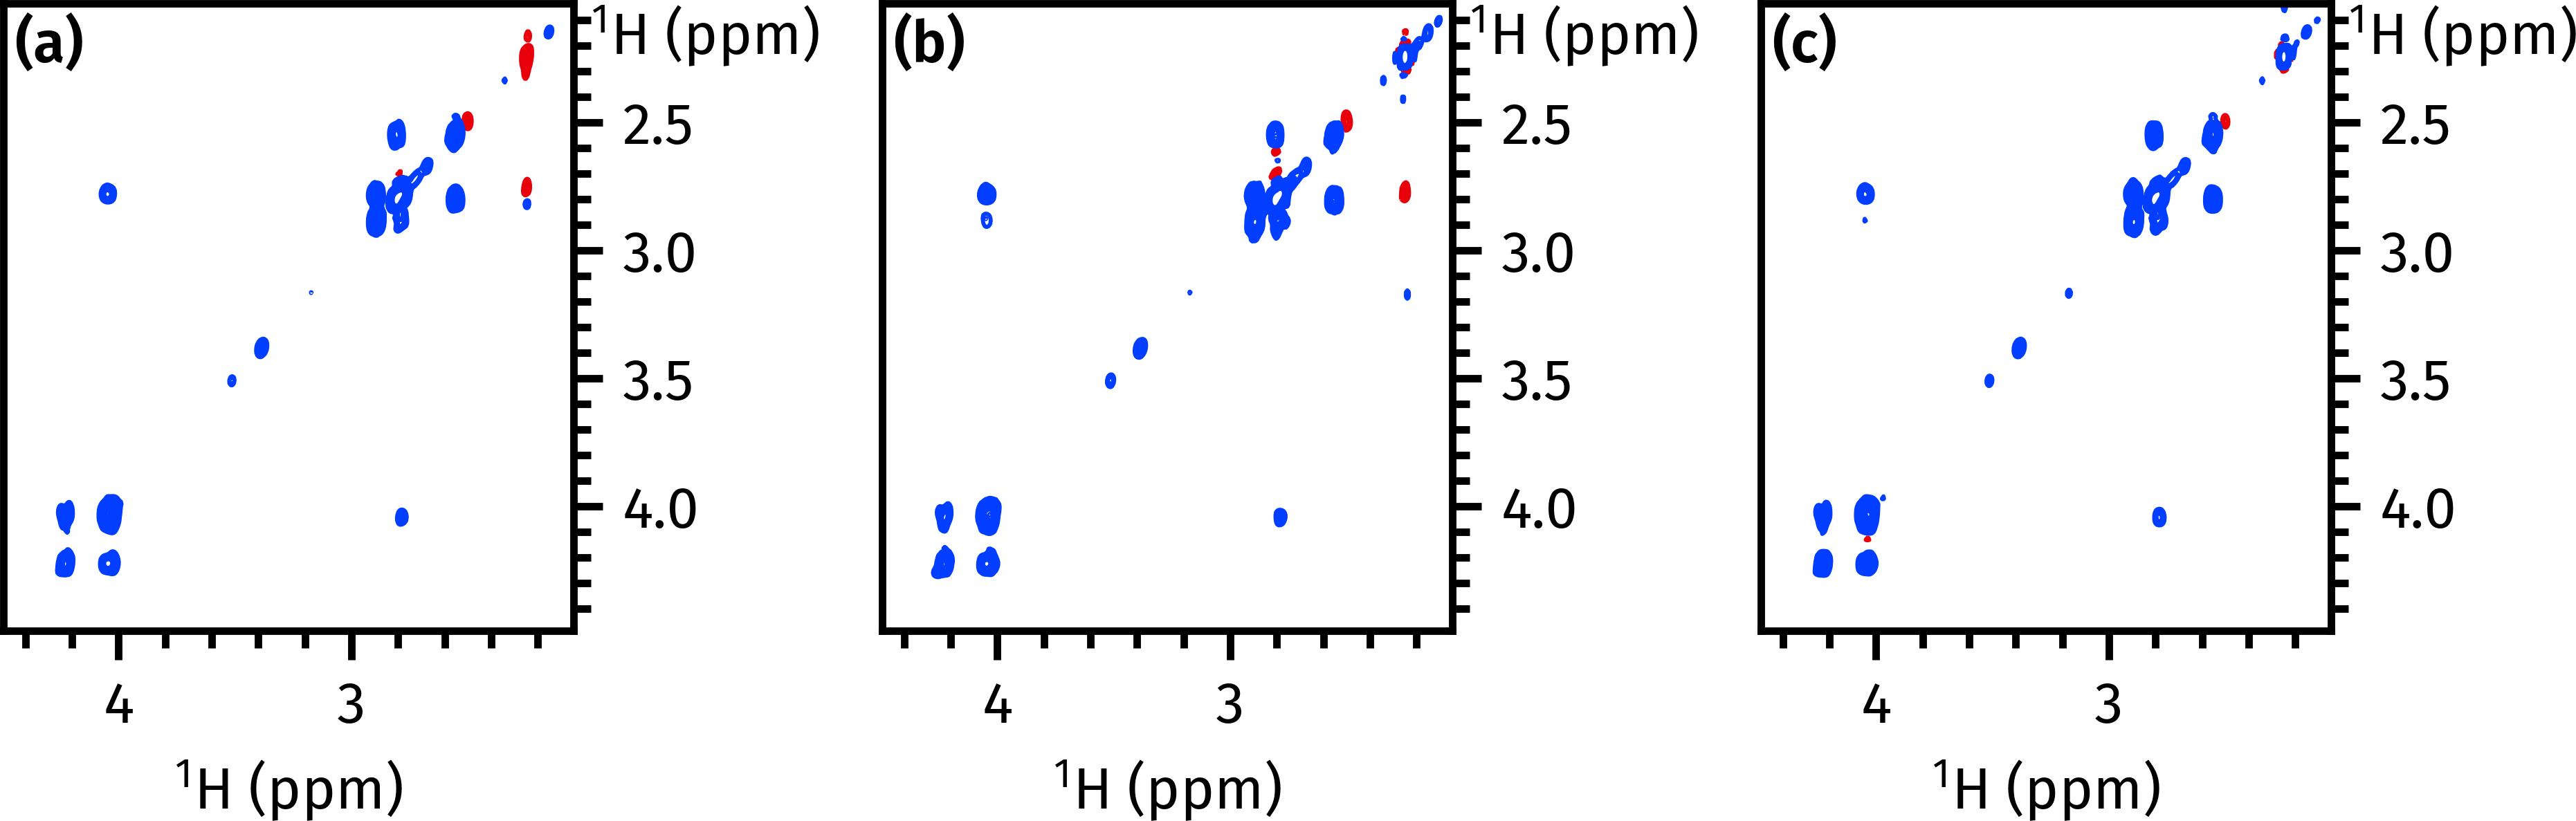
\includegraphics[]{noah/hmbc_invert_1.png}%
    {\phantomsubcaption\label{fig:hmbc_invert_1_orig}}%
    {\phantomsubcaption\label{fig:hmbc_invert_1_pw}}%
    {\phantomsubcaption\label{fig:hmbc_invert_1_bssc}}%
    \caption[Inverted peaks in homonuclear module of \noah*{B,S,X}-type supersequences]{
        \textbf{(\subref*{fig:hmbc_invert_1_orig})} CLIP-COSY from a \noah{B,S,Cc} supersequence, acquired with a \proton{} \ang{90} pulse width of \qty{11.28}{\us} (this value was obtained using the POISE calibration described in \cref{subsec:poise__pulsecal}).
        An inverted peak is visible at \qty{2.25}{\ppm}.
        \textbf{(\subref*{fig:hmbc_invert_1_pw})} The same, but acquired using a \ang{90} pulse width of \qty{11.78}{\us}.
        \textbf{(\subref*{fig:hmbc_invert_1_bssc})} CLIP-COSY from a \noah{B,S,S,Cc} supersequence. The \ang{90} pulse width was \qty{11.28}{\us}, the same as in (\subref*{fig:hmbc_invert_1_orig}).
        \datacode{7Z-220214}
    }
    \label{fig:hmbc_invert_1}
\end{figure}

The modules placed between the HMBC and the homonuclear module also play an important role.
When \textit{two} HSQC modules are used, i.e.\ a \noah{B,S,S,Cc} supersequence (using $f = 0.7$ as described in \cref{subsec:noah__hsqctocsy}---although this is unlikely to matter), the negative peaks are no longer observed (\cref{fig:hmbc_invert_1_bssc}).
In fact, having \textit{no modules} between the HMBC and the homonuclear module is also (at least sometimes) acceptable: a separate set of data shows that the inverted peaks in an \noah{B,Sp,Cc} experiment are not seen in a \noah{Sp,B,Cc} supersequence (\cref{fig:hmbc_invert_2_bspc,fig:hmbc_invert_2_spbc}).
The use of isotropic mixing (implemented as a sequence of adiabatic pulses\autocite{Kupce1998JMR}, and referred to as `ASAP' mixing) just before the homonuclear module does not remedy this (\cref{fig:hmbc_invert_2_bspc_asap,fig:hmbc_invert_2_spbc_asap}).
Unfortunately, a good explanation for these artefacts has remained elusive.

\begin{figure}[!ht]
    \centering
    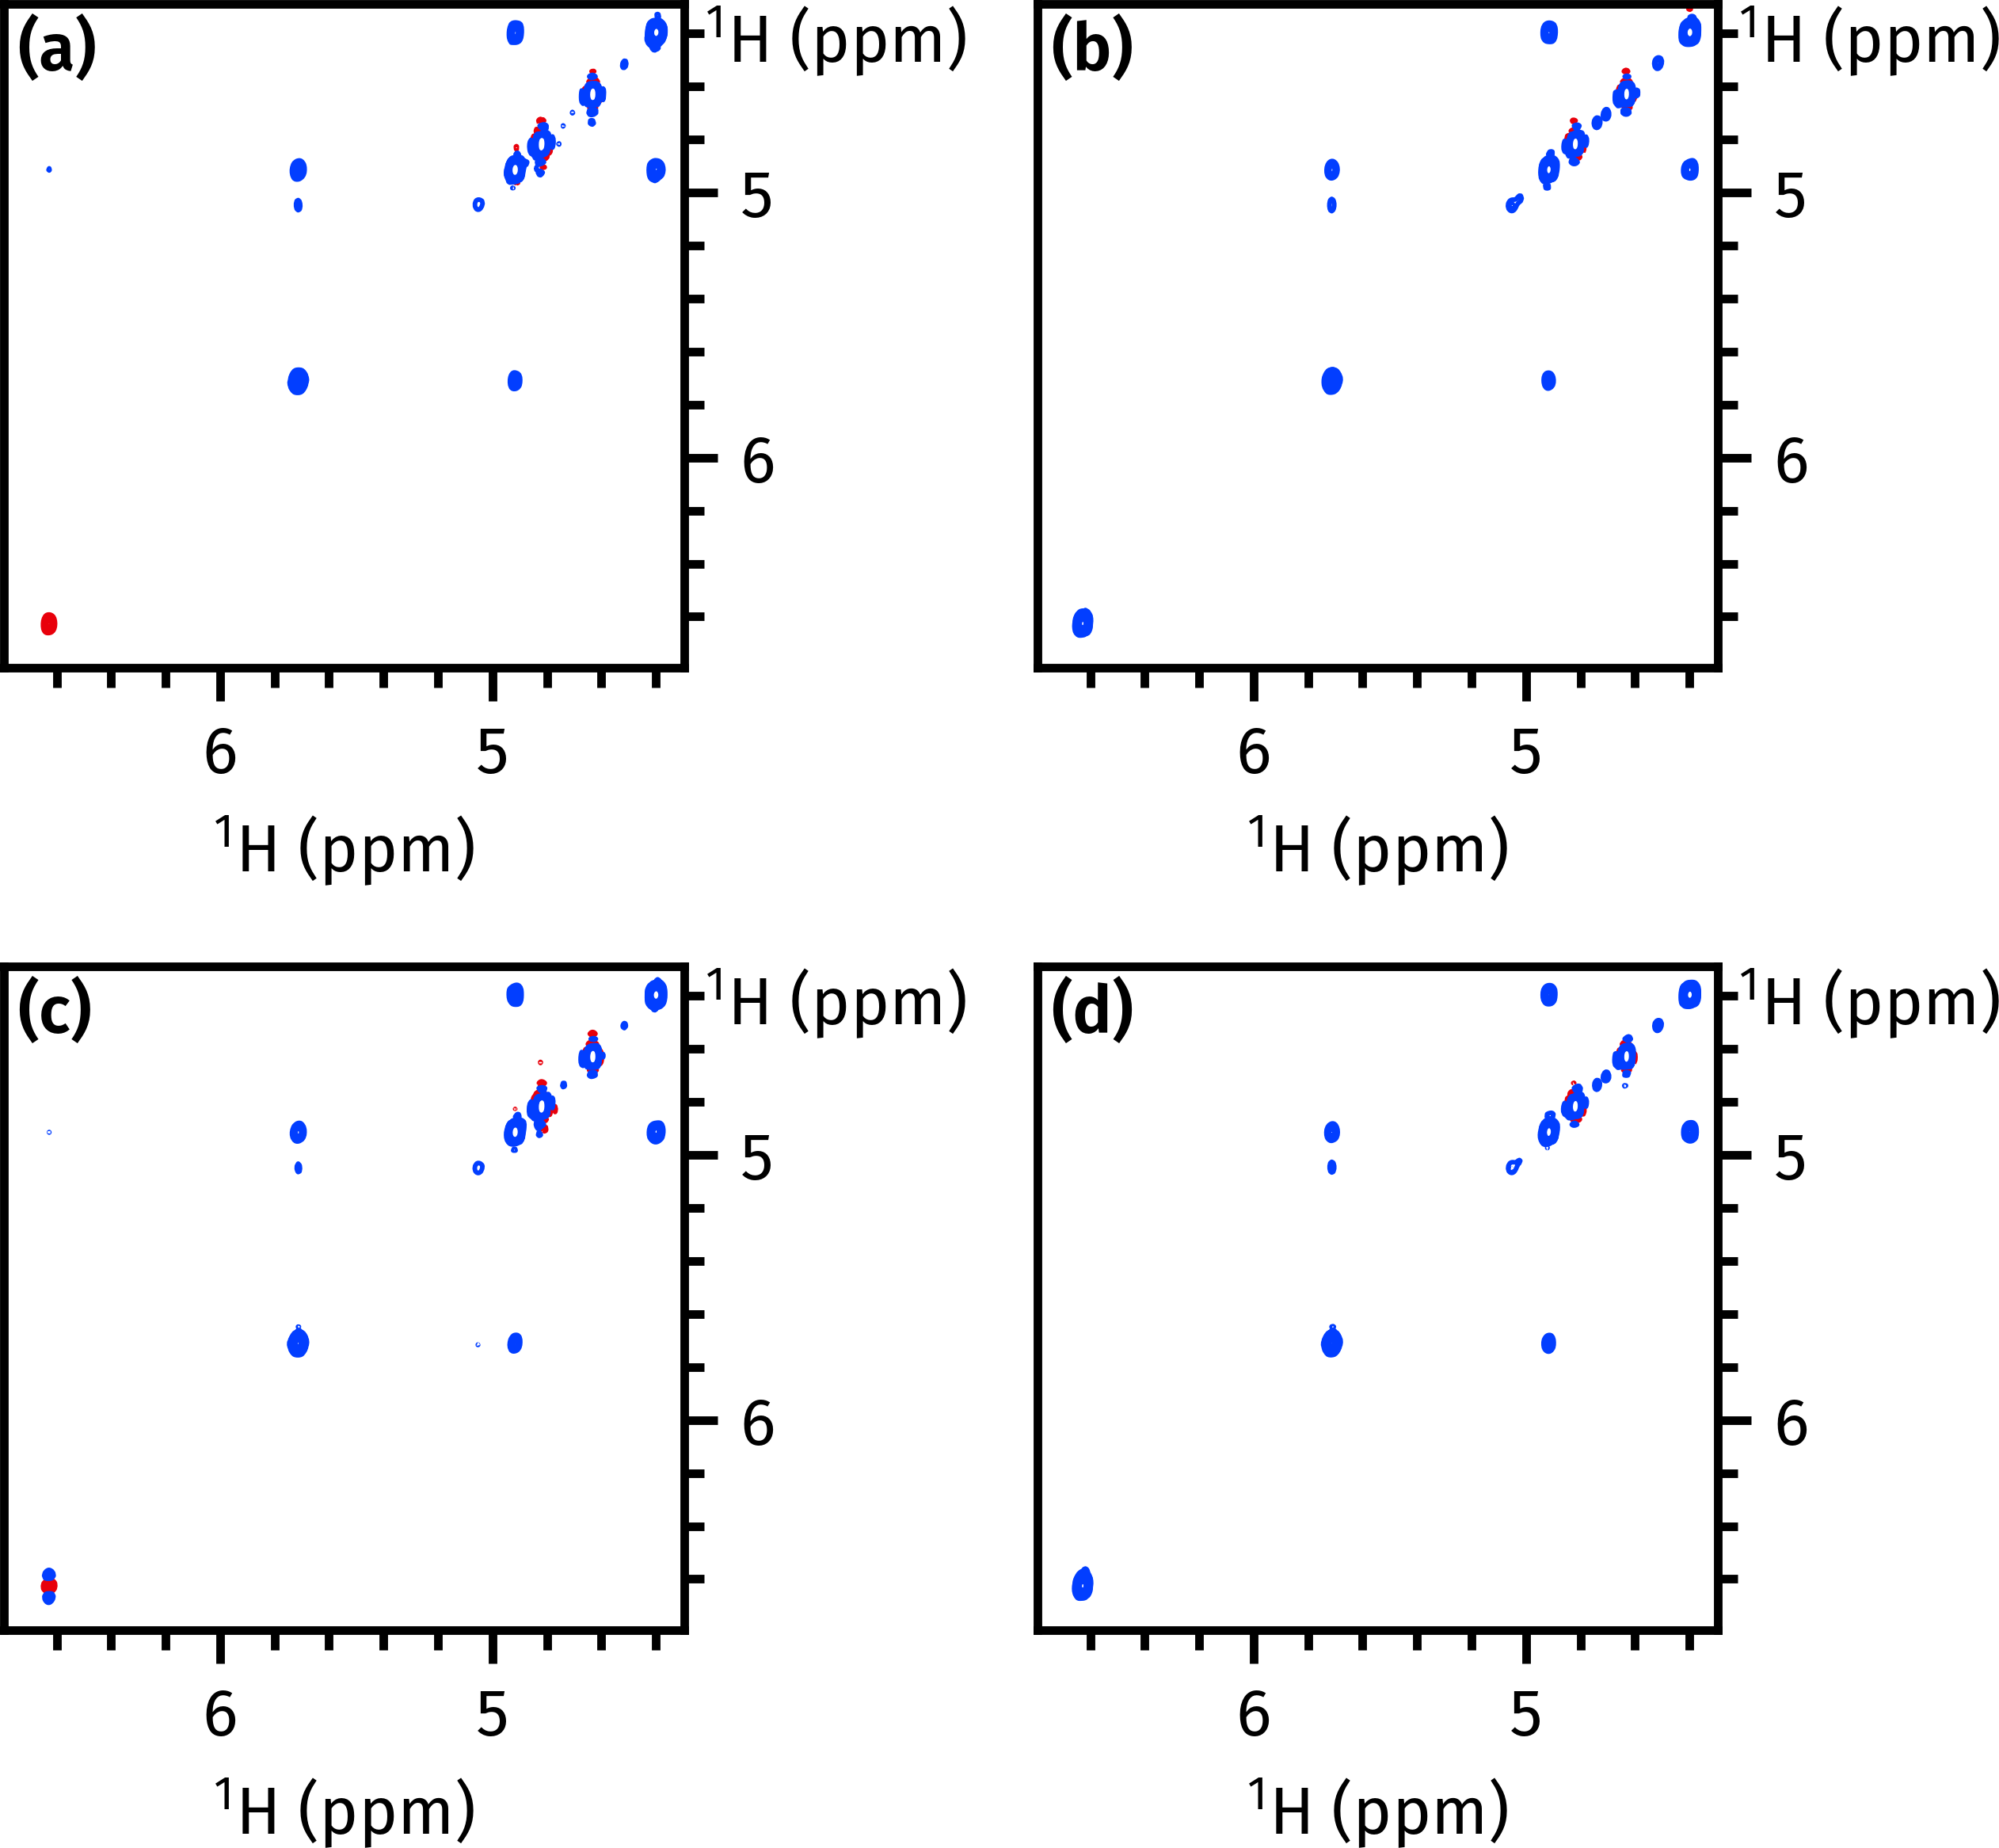
\includegraphics[]{noah/hmbc_invert_2.png}%
    {\phantomsubcaption\label{fig:hmbc_invert_2_bspc}}%
    {\phantomsubcaption\label{fig:hmbc_invert_2_spbc}}%
    {\phantomsubcaption\label{fig:hmbc_invert_2_bspc_asap}}%
    {\phantomsubcaption\label{fig:hmbc_invert_2_spbc_asap}}%
    \caption[Effect of module ordering and ASAP mixing on inverted peaks in \noah*{B,S,X}-type supersequences]{
        \textbf{(\subref*{fig:hmbc_invert_2_bspc})} CLIP-COSY from a \noah{B,Sp,Cc} supersequence.
        An inverted diagonal peak can be seen at \qty{6.6}{\ppm}.
        \textbf{(\subref*{fig:hmbc_invert_2_spbc})} From a \noah{Sp,B,Cc} supersequence.
        \textbf{(\subref*{fig:hmbc_invert_2_bspc_asap})--(\subref*{fig:hmbc_invert_2_spbc_asap})} The same as (\subref*{fig:hmbc_invert_2_bspc}) and (\subref*{fig:hmbc_invert_2_spbc}), but with \qty{40}{\ms} ASAP mixing placed just before the CLIP-COSY module.
        \datacode{7A-211227}
    }
    \label{fig:hmbc_invert_2}
\end{figure}

\subsubsection{\nitrogen{} HMBC module}

The entirety of this section has---until now---been devoted to the \carbon{} HMBC module.
However, the techniques used in constructing this, including the implementation of the $zz$-filter, are equally applicable to a \nitrogen{} HMBC.
For simplicity, the NOAH \nitrogen{} HMBC module uses a first-order LPJF (since directly bonded \ch{NH} pairs are less common); this may be omitted if desired.
To minimise the number of pulses, a simple magnitude-mode version of the HMBC is used (\cref{fig:noah_15n_hmbc}).
The implementation of this module within supersequences is discussed in greater detail within the context of \textit{generalised supersequences}, in \cref{sec:noah__parallel}.

\begin{figure}[htb]
    \centering
    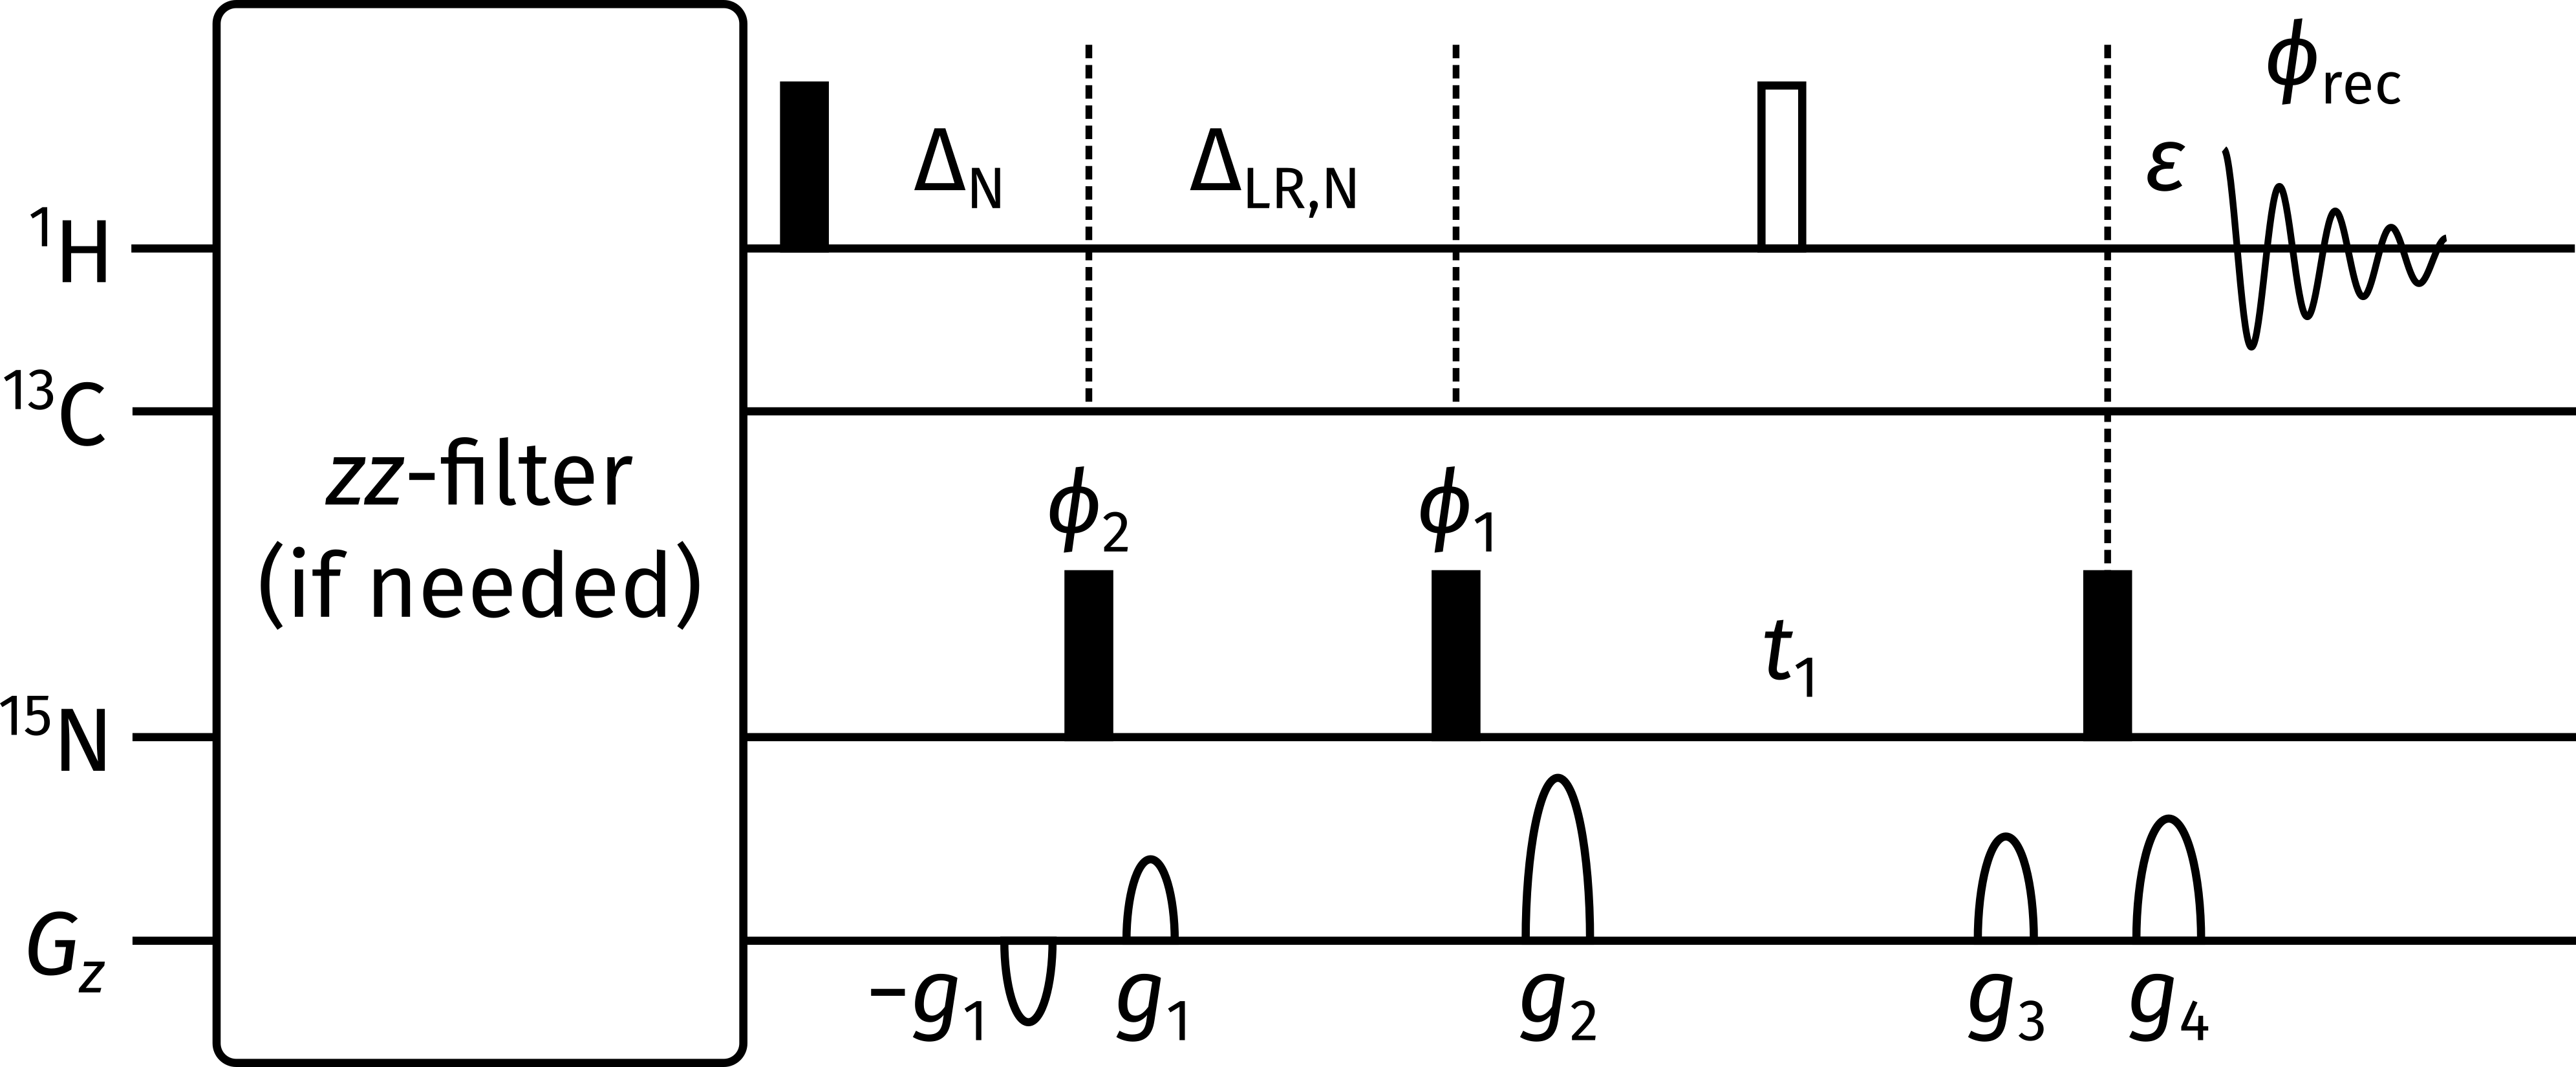
\includegraphics[]{pp/hmbc_15n.png}%
    \caption[NOAH \nitrogen{} HMBC module]{
        NOAH \nitrogen{} HMBC module.
        The $zz$-filter can be implemented as necessary in the same way as for the \carbon{} HMBC module (a final \proton{} \ang{180} pulse may also be required, but is not shown here).
        Delays are set as follows: $\Delta_{\ch{N}} = 1 / (2 \cdot \oneJ{NH})$; $\Delta_{\text{LR},\ch{N}} = 1 / (2 \cdot \nJ{NH})$.
        Phase cycling is performed using $\phi_1 = \phirec = (x, -x)$ and $\phi_2 = (x, x, -x, -x)$.
        Gradient amplitudes are $(g_1, g_2, g_3, g_4) = (5\%, 70\%, 30\%, 50.1\%)$.
    }
    \label{fig:noah_15n_hmbc}
\end{figure}

\subsection{ADEQUATE}
\label{subsec:noah__adequate}

...has inadequate sensitivity


\section{Solvent suppression in NOAH}

Blah.

\section{Parallel and generalised NOAH supersequences}
\label{sec:noah__parallel}

Blah.



\printbibliography[heading=subbibnumbered]{}
